%% Garcia's latex template for Activities Drescriptive Memorial Report
%% Version 0.2
%% (c) 2015 Vinicius Cardoso Garcia (vcg@cin.ufpe.br)
%%
%% This document is based on latex template from Prof. Daniel Cunha.
%%
%% Reference commands. Use the following commands to make references in your
%% text:
%%          \figref  -- for Figure reference
%%          \tabref  -- for Table reference
%%          \eqnref  -- for equation reference
%%          \chapref -- for chapter reference
%%          \secref  -- for section reference
%%          \appref  -- for appendix reference
%%          \axiref  -- for axiom reference
%%          \conjref -- for conjecture reference
%%          \defref  -- for definition reference
%%          \lemref  -- for lemma reference
%%          \theoref -- for theorem reference
%%          \corref  -- for corollary reference
%%          \propref -- for proprosition reference
%%          \pgref   -- for page reference
%%
%%          Example: See \chapref{chap:introduction}
%%%%%%%%%%%%%%%%%%%%%%%%%%%%%%%%%%%%%%%%%%%%%%%%%%%%%%%%%%%%%%%%%%%%%%%%%%%%%%%

\documentclass[a4paper,oneside,10pt]{article}

\usepackage[latin1,utf8]{inputenc}
\usepackage[T1]{fontenc}
\usepackage[brazilian]{babel}

\usepackage{graphicx}
\usepackage{amsmath,amstext,amssymb,amsfonts}
\usepackage[none]{hyphenat}
\usepackage{fancyhdr}
\usepackage{cite}
\usepackage{indentfirst}
%\usepackage{path}
\usepackage[usenames, dvipsnames]{color}

\usepackage{pdfsync}
\usepackage{url}
\usepackage{setspace}

\usepackage{colortbl}
\newcommand{\SetRowColor}[1]{\noalign{\gdef\RowColorName{#1}}\rowcolor{\RowColorName}}

\definecolor{MyRed}{rgb}{1,0.2,0.1}
\definecolor{light-gray}{gray}{0.95}
\definecolor{gray}{gray}{0.6}

\usepackage{booktabs}
\usepackage{ctable}
\usepackage{setspace}
\usepackage[multidot]{grffile}
\usepackage[final]{pdfpages}

\usepackage{titlesec}

\usepackage[toc,page]{appendix}
\newcommand{\appref}[1]{\@appendixname~\ref{#1}\xspace}
%\usepackage{xifthen}

% ricardoaf
\usepackage{float}
\usepackage{makecell}
\usepackage{ragged2e}
%\usepackage[hidelinks]{hyperref}
%\usepackage{multirow}
%\usepackage{longtable}
%\usepackage{threeparttable}
%\usepackage{textcomp}
%\usepackage{array}
%\newcolumntype{C}[1]{>{\centering\arraybackslash}m{#1}}
%\newcolumntype{P}[1]{>{\RaggedRight\arraybackslash\hspace{0pt}}p{#1}}
%\usepackage{pdflscape}
\usepackage{longtable,array}
%\newcolumntype{P}[1]{>{\RaggedRight\arraybackslash\hspace{0pt}}p{#1}}
\newcolumntype{P}[1]{>{\RaggedRight\arraybackslash}p{#1}}


\usepackage[bookmarks,pdfpagelabels,
pdftitle={Relatório de Desempenho Acadêmico}, pdfauthor={Eduardo Setton S. da Silveira},
pdfsubject={Solicitação de progressão funcional docente de Associado Nível 4 para Professor Titular apresentada à Comissão Interna de Avaliação de Progressão da Universidade Federal de Alagoas.},
pdfcreator={Eduardo Setton S. da Silveira}, pdfkeywords={Progressão, Titular, UFAL, CTEC, Docente}]{hyperref}

\newcommand{\otoprule}{\midrule[\heavyrulewidth]}

% Definição de margens
\setlength{\textwidth}{16cm} %
\setlength{\textheight}{23cm} %
\setlength{\oddsidemargin}{0cm} %
\setlength{\evensidemargin}{0cm} %
\setlength{\topmargin}{0cm}

\renewcommand{\abstractname}{Resumo}
\renewcommand{\contentsname}{Índice Analítico}
\renewcommand{\refname}{Referências}
\renewcommand{\appendixname}{Apêndice}
\renewcommand{\tablename}{Tabela}

%% Formatação do cabeçalho e rodapé
\lhead{\footnotesize Relatório de Desempenho Acadêmico} %
\rhead{\footnotesize \emph{Eduardo Setton Sampaio da Silveira}} %
\chead{} %
\cfoot{} %
\lfoot{\footnotesize\nouppercase\leftmark} %
\rfoot{\bfseries\thepage}
\renewcommand{\footrulewidth}{0.1pt}

% Comando para inserir número de documento
\newcounter{document}%[section]
\setcounter{document}{0}
\renewcommand\theenumi{\arabic{section}.\arabic{enumi}}
\newcommand\Doc{{\addtocounter{document}{1}\mbox{\sffamily\bfseries [Doc. \arabic{document}]}}}

% Comando para repetir um número de documento já citado
% \mbox{\sffamily{\bfseries{[Doc. XX]}}}

%% Alternativa na edição dos comandos.
%% Comando para inserir número de documento
% \newcommand\thedocument{%
%    \ifthenelse{\arabic{subsection}=0}
%      {\thesection.\arabic{document}}
%      {\thesubsection.\arabic{document}}}
% \newcounter{document}[section]
% \setcounter{document}{0}
% \renewcommand\theenumi{\arabic{section}.\arabic{enumi}}
% \ifthenelse{\arabic{subsection} = 0}{\newcommand\Doc{{\stepcounter{document}\bfseries [Doc. \arabic{section}.\arabic{document}]}}}{\newcommand\Doc{{\stepcounter{document}\bfseries [Doc. \arabic{section}.\arabic{subsection}.\arabic{document}]}}}
% %\newcommand\Doc{{\addtocounter{document}{1}\mbox{\bfseries [Doc. \arabic{document}]}}}

% Ambiente para centralizar vertical
\newenvironment{vcenterpage}
     {\newpage\vspace*{\fill}}
     {\vspace*{\fill}\par\pagebreak}

\sloppy

\pagestyle{fancy}

\setcounter{secnumdepth}{4}

\begin{document}

\begin{titlepage}

\vspace{-5.0cm}

\begin{figure}[!htb]
 \centering{\includegraphics[scale=2.0]{logo-ctec.pdf}}
 \label{fig:UFAL_CTEC_logo}
\end{figure}

\begin{center}
\vspace{1cm}
%{\huge \textsf{Solicitação de Progressão Funcional Docente}} \\[1cm]
\rule{1.0\textwidth}{1pt} \\ [0.5cm]
{\Huge \textbf{\textsf{Relatório de Desempenho Acadêmico}}} \\
\rule{1.0\textwidth}{1pt} \\
\vspace{2cm}

\doublespacing
{\Large \textsf{Solicitação de progresssão funcional docente de \textbf{Associado Nível 4 para Professor Titular} apresentada à Comissão de Avaliação de Progressão do Centro de Tecnologia da Universidade Federal de Alagoas}}\\
\vspace{1.5cm}
{\LARGE \textsf{Solicitante: \textbf{Eduardo Setton Sampaio da Silveira}}}\\
\vspace{0.5cm}
{\Large \textsf{SIAPE: \textbf{1140981}}} \\
\vspace{0.5cm}
{\Large \textsf{Período: \textbf{25/03/2016 - 24/03/2018}}} \\

\vspace{2.0cm}

\normalsize \textsf{Janeiro de 2018}

\end{center}
\thispagestyle{empty}
\end{titlepage}

\tableofcontents
%\include{Lista_Anexos} \cleartooddpage[\thispagestyle{empty}]

%%%%%%%%%%%%%%%%%%%%%%%%%%%%%%%%%%%%%%%%%%%%%%%%%%%%%%%%%%%%%%%%%%%%%%%%%%%%%%%
% APRESENTAçãO
%%%%%%%%%%%%%%%%%%%%%%%%%%%%%%%%%%%%%%%%%%%%%%%%%%%%%%%%%%%%%%%%%%%%%%%%%%%%%%%

\newpage
\section*{Apresentação}
\vspace{0.3cm}

\begin{onehalfspace}

Memorial apresentado por \textbf{Eduardo Setton Sampaio da Silveira}, Professor Associado 4, lotado no Centro de Tecnologia (CTEC) da Universidade Federal de Alagoas (UFAL), para avaliação de desempenho acad\^{e}mico, para fins de acesso por progressão à classe E, com denominação de Professor Titular.

O presente memorial relata as atividades desempenhadas no período de \textbf{25 de Março de 2016 a 24 de Março de 2018} e foi elaborado com base nas diretrizes estabelecidas nas Resoluções 78/2014 do Conselho Universitário (CONSUNI) da UFAL, de 17/11/2014  e na Portaria 554, de 20/06/2013, do Ministério da Educação (MEC). Os documentos comprobatórios referenciados neste memorial estão organizados em volumes anexos devidamente numerados. Por fim, os Anexos que se referem a artigos publicados em confer\^{e}ncias e periódicos contém apenas a primeira página do trabalho e o email informando a aceitação do trabalho para publicação (quando pertinente).

Em atendimento aos requisitos I e II estabelecidos na Resolução 78/2014 do Conselho Universitário (CONSUNI) da UFAL, de 17/11/2014, que determinam, respectivamente, à exigência da posse do Título de Doutor e o cumprimento de insterstício mínimo de (vinte e quatro) meses de efetivo exercício no nível 4 da Classe D (D-IV) os dois primeiros documentos apresentados no anexo relativo aos documentos comprobatórios estão: o diploma de doutorado \mbox{\sffamily{\bfseries{[Doc. \ref{doutorado:diploma}]}}} e as portarias referentes ao interstício cumprido pelo docente como Professor Associado IV \mbox{\sffamily{\bfseries{[Doc. \ref{portaria:associadoiv}]}}}.

Ainda em atendimento a esta resolução, o avaliando faz a opção pela avaliação do relatório de desempenho acadêmico para os três primeiros grupos de atividade com os percentuais estabelecidos abaixo:\\
\begin{itemize}
\item \textbf{Grupo I - Atividades de Ensino:} 40\%
\item \textbf{Grupo II - Produção Intelectual:} 30\%
\item \textbf{Grupo III - Atividades de Pesquisa:} 30\%
\end{itemize}

\end{onehalfspace}

%\subsection*{Esclarecimentos}

%Aqui nesta seção especial podem ser listadas algumas observações acerca da %documentação comprobatória para dirimir possíveis dúvidas da Comissão %Avaliadora. A numeração indicada corresponde à numeração do Anexo.

%\begin{itemize}

%\item [18.] Artigo disponível em \verb"dx.doi.org/10.14209/sbrt.2013.182".
%\item [19.] Lista de artigos aceitos disponível em \verb"http://www.sbrt.org.br/%sbrt2012/artigos.html". O artigo em questão possui identificação 98879.
%\item E assim por diante.

%\end{itemize}


%%%%%%%%%%%%%%%%%%%%%%%%%%%%%%%%%%%%%%%%%%%%%%%%%%%%%%%%%%%%%%%%%%%%%%%%%%%%%%%
% Grupo 1 - Atividades de Ensino
%%%%%%%%%%%%%%%%%%%%%%%%%%%%%%%%%%%%%%%%%%%%%%%%%%%%%%%%%%%%%%%%%%%%%%%%%%%%%%%
\newpage
\section{Atividades de Ensino}
%A seguir, listo as atividades de ensino que realizei no período, separadas por subgrupo, conforme rege o documento tal.

%%%%%%%%%%%%%%%%%%%%%%%%%%%%%%%%%%%%%%%%%%%%%%%%%%%%%%%%%%%%%%%%%%%%%%%%%%%%%%%
% Subgrupo 1.1 - Ministração de aula
%%%%%%%%%%%%%%%%%%%%%%%%%%%%%%%%%%%%%%%%%%%%%%%%%%%%%%%%%%%%%%%%%%%%%%%%%%%%%%%
\subsection{Ministração de aula}
\vspace{0.3cm}

Na Tabela \ref{Tab:Disc_Grad}, estão listadas as disciplinas ministradas nos cursos de graduação e de pós-graduação  no período de 25/03/2016 a 24/03/2018. As disciplinas estão organizadas por semestre, com a identificação do curso, da turma e da disciplina, esta última com sua respectiva carga horária. Adicionalmente, consta na referida Tabela a carga horária média semestral ao longo do período de avaliação.

{\setlength{\tabcolsep}{0.1cm}
\begin{table}[H]
\centering \small
\caption{\texttt{Disciplinas de graduação lecionadas no período considerado} }
\def\arraystretch{1.5}
\resizebox{\textwidth}{!}{
\begin{tabular}{cccccc}
\toprule
\textbf{Semestre} & \textbf{Curso} & \textbf{Turma} & \textbf{Disciplina} & \textbf{C.H.} &\textbf{Doc} \\
\otoprule
  & Eng. Civil & $D$ & ECIV005 - Introdução à Engenharia & 30 & \ref{disciplinas:doc1}\\
$2015.2$ & Eng.de Petróleo & $A$ & EPET006 - Introdução à Computação & 60 & \ref{disciplinas:doc2}\\
  & Eng. de Petróleo & $A$ & EPET070 - Aval. Econômica de Projetos em Óleo e Gás & 30 & \ref{disciplinas:doc2}\\
\cmidrule{1-6}
\multicolumn{4}{r}{\textbf{Carga Horária Total do Semestre}} & \textbf{120} \\
\otoprule
  & Eng.Ambiental & $A$ & EAMB069 - Administração & 30 & \ref{disciplinas:doc5}\\
$2016.1$ & Eng.Civil & $A$ & ECIV005 - Introdução à Engenharia  & 30 & \ref{disciplinas:doc1}\\
  & Eng.Civil & $A$ & ECIV074 - Administração & 30 &  \ref{disciplinas:doc1}\\
  & Eng.Petróleo & $A$ &  EPET006 - Introdução à Computação & 60 & \ref{disciplinas:doc2}\\
  & Eng.Petróleo & $A$ & EPET070 - Aval. Econômica de Projetos em Óleo e Gás & 30 & \ref{disciplinas:doc2}\\
\cmidrule{1-6}
\multicolumn{4}{r}{\textbf{Carga Horária Total do Semestre}} & \textbf{150} \\
\otoprule
& Eng.Ambiental & $B$ & EAMB069 - Administração & 30 & \ref{disciplinas:doc5}\\
  & Eng.Civil & $D$ & ECIV005 - Introdução à Engenharia  & 30 & \ref{disciplinas:doc1}\\
  & Eng.Civil & $D$ & ECIV074 - Administração & 30 & \ref{disciplinas:doc1}\\
  $2016.2$ & Eng.Petróleo & $A$ &  EPET006 - Introdução à Computação & 60 & \ref{disciplinas:doc3}\\
  & Eng.Petróleo & $A$ & EPET070 - Aval. Econômica de Projetos em Óleo e Gás & 30 & \ref{disciplinas:doc3}\\
  & PROFNIT & $A$ & \makecell{PROFNIT05 - Políticas Públicas de CTI e o Estado Brasileiro} & 15 & \ref{disciplinas:doc6profnit}\\
\cmidrule{1-6}
\multicolumn{4}{r}{\textbf{Carga Horária Total do Semestre}} & \textbf{165} \\
\otoprule
& Eng.Ambiental & $A$ & EAMB069 - Administração & 30 & \ref{disciplinas:doc5}\\
& Eng.Civil & $A$ & ECIV005 - Introdução à Engenharia  & 30 & \ref{disciplinas:doc1}\\
  & Eng.Civil & $A$ & ECIV074 - Administração & 30 & \ref{disciplinas:doc1}\\
 $2017.1$ & Eng.de Petróleo & $A$ &  EPET006 - Introdução à Computação & 60 & \ref{disciplinas:doc3}\\
  & Eng.Petróleo & $A$ & EPET070 - Aval. Econômica de Projetos em Óleo e Gás & 30 & \ref{disciplinas:doc3}\\
   & PROFNIT & $A$ & \makecell{PROFNIT05 - Políticas Públicas de CTI e o Estado Brasileiro} & 15 & \ref{disciplinas:doc6profnit}\\
   & PROFNIT & $A$ & PROFNIT04 -Metodologia da Pesquisa CTI & 15 & \ref{disciplinas:doc6profnit}\\
\cmidrule{1-6}
\multicolumn{4}{r}{\textbf{Carga Horária Total do Semestre}} & \textbf{180} \\
\otoprule
 & Eng.Ambiental & $B$ & EAMB069 - Administração & 30 & 1\\
  & Eng.Civil & $D$ & ECIV005 - Introdução à Engenharia  & 30 & 1\\
$2017.2$  & Eng.Civil & $D$ & ECIV074 - Administração & 30 & 1\\
  & Eng.Petróleo & $A$ &  EPET006 - Introdução à Computação & 60 & 1\\
  & Eng.Petróleo & $A$ & EPET070 - Aval. Econômica de Projetos em Óleo e Gás & 30 & 1\\
  & Eng.Petróleo & $A$ & EPET096 - Administração & 30 & 1\\
\cmidrule{1-6}
\multicolumn{4}{r}{\textbf{Carga Horária Total do Semestre}} & \textbf{150} \\
\cmidrule{1-6}
\multicolumn{4}{r}{\textbf{Carga Horária Total Ministrada no Período}} & \textbf{765} \\
\bottomrule
\end{tabular}
\label{Tab:Disc_Grad}
}
\end{table}}


%%%%%%%%%%%%%%%%%%%%%%%%%%%%%%%%%%%%%%%%%%%%%%%%%%%%%%%%%%%%%%%%%%%%%%%%%%%%%%%
% Subgrupo 1.1 - Orientação
%%%%%%%%%%%%%%%%%%%%%%%%%%%%%%%%%%%%%%%%%%%%%%%%%%%%%%%%%%%%%%%%%%%%%%%%%%%%%%%
\subsection{Orientação}
\vspace{0.3cm}

\subsubsection{Orientação concluída de estudante em Trabalho de Conclusão de Curso}
\vspace{0.3cm}

\begin{enumerate}
\renewcommand{\labelenumi}{{\large\bfseries\arabic{enumi}.}}

\item  \textbf{Aluno:} : Josué Domingos da Silva Neto \mbox{\sffamily{\bfseries{[Doc. \ref{tcc:doc7}]}}}\\
            \textbf{Curso:} Engenharia de Petróleo\\
            \textbf{Título da Monografia:} A Indústria do Petróleo no Brasil e no Mundo: Modelos de Contrato para Exploração e Produção \\
            \textbf{Defesa:} Maio de 2017\\
            \textbf{Instituição:} Universidade Federal de Alagoas
            
\item  \textbf{Aluno:} Kerolaye Ancelmo da Silva \mbox{\sffamily{\bfseries{[Doc. \ref{tcc:doc8}]}}}\\
            \textbf{Curso:} Engenharia Civil\\
            \textbf{Título da Monografia:} Aplicação da Metodologia Matriz SWOT para Diagnóstico e Proposição de Soluções Das Obras Definidas No PNLT Em Alagoas\\
            \textbf{Defesa:} Dezembro de 2017\\
            \textbf{Instituição:} Universidade Federal de Alagoas
\end{enumerate}

%------------------------------------------------------------------------------

\subsubsection{Supervisão direta de estágios curriculares}
\vspace{0.3cm}

\begin{enumerate}
\renewcommand{\labelenumi}{{\large\bfseries\arabic{enumi}.}}

\item   \textbf{Estagiário:} : Josué Domingos da Silva Neto) \mbox{\sffamily{\bfseries{[Doc. \ref{advisor:estagio}]}}} \\
            \textbf{Local do estágio:} Laboratório de Computação Científica e Visualização \\
            \textbf{Data de Início:} 23 de Janeiro de 2017 \\
            \textbf{Data de Término:} 24 de Abril de 2017 \\
            \textbf{Jornada de trabalho:} 20 horas semanais \\
            \textbf{Total de horas:} 252 horas em 63 dias \\
            \textbf{Instituição:} LCCV/CTEC/UFAL

\end{enumerate}

%------------------------------------------------------------------------------

\subsubsection{Supervisão e acompanhamento de monitorias}
\vspace{0.3cm}

\begin{enumerate}
\renewcommand{\labelenumi}{{\large\bfseries\arabic{enumi}.}}

\item       \textbf{Aluno:} Jonathan Ferreira Francisco \mbox{\sffamily{\bfseries{[Doc. \ref{orient:monitoria1}]}}}\\
                \textbf{Disciplina:}  Introdução à Computação\\
                \textbf{Curso:} Engenharia de Petróleo\\
                \textbf{Semestres:} 2016.1\\
                \textbf{Instituição:} CTEC/UFAL

\item       \textbf{Aluno:} Andressa Amancio dos Santos \mbox{\sffamily{\bfseries{[Doc. \ref{orient:monitoria2}]}}}\\
               \textbf{Disciplina:}  Introdução à Computação\\
               \textbf{Curso:} Engenharia de Petróleo\\
               \textbf{Semestres:} 2017.1\\
               \textbf{Instituição:} CTEC/UFAL
            
\item       \textbf{Aluno:} Renato Ramos de Lima dos Santos \mbox{\sffamily{\bfseries{[Doc. \ref{orient:monitoria3}]}}}\\
               \textbf{Curso:} Engenharia de Petróleo\\
               \textbf{Semestres:} 2017.1\\
               \textbf{Instituição:} CTEC/UFAL
\end{enumerate}

%------------------------------------------------------------------------------

\newpage
\subsubsection{Orientação de dissertação de Mestrado em andamento, por semestre}
\vspace{0.3cm}

\begin{enumerate}
\renewcommand{\labelenumi}{{\large\bfseries\arabic{enumi}.}}

\item   \textbf{Aluna:} Danyella Nutels Reys \mbox{\sffamily{\bfseries{[Doc. \ref{advisor:msc-andamento}]}}} \\
            \textbf{Título da Dissertação:} Estudo setorial e tecnológico da Indústria de óculos e desenvolvimento de modelo de negócios através da impressora 3D\\
            \textbf{Curso:} Programa de Pós-Graduação em Propriedade Intelectual e Transferência de Tecnologia para a Inovação \\%| Profissional\\
            \textbf{Tipo:} Profissional \\%| Profissional\\
            \textbf{Data de Início:} 29 de Maio de 2017\\
            \textbf{Instituição:} UFAL.

\item   \textbf{Aluna:} Nádia Teresinha Paim Corso \mbox{\sffamily{\bfseries{[Doc. \ref{advisor:msc-andamento}]}}} \\
            \textbf{Título da Dissertação:} Modelo de Sistema de Gestão da Propriedade Intelectual e da Transferência de Tecnologia no Laboratório de Computação Científica e Visualizacão - LCCV\\
            \textbf{Curso:} Programa de Pós-Graduação em Propriedade Intelectual e Transferência de Tecnologia para a Inovação \\%| Profissional\\
            \textbf{Tipo:} Profissional \\%| Profissional\\
            \textbf{Data de Início:} 21 de Setembro de 2017\\
            \textbf{Instituição:} UFAL.
            
\item   \textbf{Aluna:} Renata Fonseca de Gomes Pereira \mbox{\sffamily{\bfseries{[Doc. \ref{advisor:msc-andamento}]}}} \\
            \textbf{Título da Dissertação:} Marcas: Ativo Intangível ou Prejuízo Tangível\\
            \textbf{Curso:} Programa de Pós-Graduação em Propriedade Intelectual e Transferência de Tecnologia para a Inovação \\%| Profissional\\
            \textbf{Tipo:} Profissional \\%| Profissional\\
            \textbf{Data de Início:} 21 de Setembro de 2017\\
            \textbf{Instituição:} UFAL.            
      
\item   \textbf{Aluno:} Tiago Alves Nogueira de Souza \mbox{\sffamily{\bfseries{[Doc. \ref{advisor:msc-andamento}]}}} \\
            \textbf{Título da Dissertação:} Utilização de Data Science para predição de informações a partir de radares meteorológicos\\
            \textbf{Curso:} Programa de Pós-Graduação em Propriedade Intelectual e Transferência de Tecnologia para a Inovação \\%| Profissional\\
            \textbf{Tipo:} Profissional \\%| Profissional\\
            \textbf{Data de Início:} 21 de Setembro de 2017\\
            \textbf{Instituição:} UFAL.  
          
\item  \textbf{Aluno:} Alcilene Vieira Ferreira \mbox{\sffamily{\bfseries{[Doc. \ref{advisor:msc-andamento}]}}} \\
            \textbf{Título da Dissertação:} Gestão da Comunicação para Inovação: estudo de caso da Rede Metrológica de Alagoas\\
            \textbf{Curso:} Programa de Pós-Graduação em Propriedade Intelectual e Transferência de Tecnologia para a Inovação \\%| Profissional\\
            \textbf{Tipo:} Profissional \\%| Profissional\\
            \textbf{Data de Início:} 21 de Setembro de 2017\\
            \textbf{Instituição:} UFAL.  
             
\item   \textbf{Aluno:} Raphael Bezerra Falcão de Almeida \mbox{\sffamily{\bfseries{[Doc. \ref{advisor:msc-andamento}]}}} \\
            \textbf{Título da Dissertação:} Proposição de estratégias de inserção de comunidades e associações carentes no mundo digital: Estudo de caso de um negócio de impacto social \\
            \textbf{Curso:} Programa de Pós-Graduação em Propriedade Intelectual e Transferência de Tecnologia para a Inovação \\%| Profissional\\
            \textbf{Tipo:} Profissional \\%| Profissional\\
            \textbf{Data de Início:} 21 de Setembro de 2017\\
            \textbf{Instituição:} UFAL.  
            
\end{enumerate}

%------------------------------------------------------------------------------

\newpage
\subsubsection{Co-orientação de dissertação de Mestrado em andamento, por semestre}
\vspace{0.3cm}

\begin{enumerate}
\renewcommand{\labelenumi}{{\large\bfseries\arabic{enumi}.}}

\item   \textbf{Aluno:} Edilson Ponciano de Lima \mbox{\sffamily{\bfseries{[Doc. \ref{advisor:mscco-andamento}]}}} \\
            \textbf{Título da Dissertação:} Desenvolvimento de Aplicativo de Alerta Tecnológico de Depósito de Patentes na Base do INPI \\
            \textbf{Curso:} Programa de Pós-Graduação em Propriedade Intelectual e Transferência de Tecnologia para a Inovação \\%| Profissional\\
            \textbf{Tipo:} Profissional \\%| Profissional\\
            \textbf{Data de Início:} 21 de Setembro de 2017 \\
            \textbf{Instituição:} UFAL.  
            
            \item   \textbf{Aluno:} Pedro Henrique Oliveira Silva\mbox{\sffamily{\bfseries{[Doc. \ref{advisor:mscco-andamento}]}}} \\
            \textbf{Título da Dissertação:} Metodologia de Desenvolvimento das Competências de Inovação em Integrantes de Redes Colaborativas\\
            \textbf{Curso:} Programa de Pós-Graduação em Propriedade Intelectual e Transferência de Tecnologia para a Inovação \\%| Profissional\\
            \textbf{Tipo:} Profissional \\%| Profissional\\
            \textbf{Data de Início:} 21 de Setembro de 2017\\
            \textbf{Instituição:} UFAL.  
            

\end{enumerate}

%------------------------------------------------------------------------------

\subsubsection{Orientação de estudantes de graduação em programas institucionalizados de pesquisa em andamento, por semestre}
\vspace{0.3cm}

\begin{enumerate}
\renewcommand{\labelenumi}{{\large\bfseries\arabic{enumi}.}}

\item    \textbf{Aluno:} Carolynne Morgana Leite Ferro \mbox{\sffamily{\bfseries{[Doc. \ref{advisor:ict-lccv1}]}}} \\
             \textbf{Projeto:}  Laboratório de Computação Científica e Visualização
             \textbf{Tema:} Planjejamento e Gestão da Inovação no LCCV/UFAL\\
             \textbf{Data de Início:} 01 de Agosto de 2016\\
             \textbf{Financiamento:} LCCV/UFAL
             
 \item    \textbf{Aluno:} Marco Magnano \mbox{\sffamily{\bfseries{[Doc. \ref{advisor:ict-lccv2}]}}} \\
             \textbf{Projeto:}  Laboratório de Computação Científica e Visualização
             \textbf{Tema:} Geopolítica na Análise de Dados Históricos de Produção de Petróleo: Uma Perspectiva Global \\
             \textbf{Data de Início:} 01 de Agosto de 2016\\
             \textbf{Financiamento:} LCCV/UFAL
             
\item    \textbf{Aluno:} Gustavo Coelho Lopes \mbox{\sffamily{\bfseries{[Doc. \ref{advisor:ict-pibit}]}}} \\
             \textbf{Projeto:} Ferramenta  Computacional Baseada em Ciência dos Dados para Petróleo e Gás - Data Science for Oil \\
             \textbf{Tema:} Modelo de Negócios \\
             \textbf{Data de Início:} 01 de Agosto de 2017\\
             \textbf{Financiamento:} PIBIT/UFAL

\item    \textbf{Aluno:} Renato Ramos de Lima dos Santos \mbox{\sffamily{\bfseries{[Doc. \ref{advisor:ict-pibit}]}}} \\
             \textbf{Projeto:} Ferramenta  Computacional Baseada em Ciência dos Dados para Petróleo e Gás - Data Science for Oil \\
             \textbf{Tema:} Implementação da ferramenta \\
             \textbf{Data de Início:} 01 de Agosto de 2017\\
             \textbf{Financiamento:} PIBIT/UFAL
             
  \item    \textbf{Aluna:} Andressa Amancio dos Santos \mbox{\sffamily{\bfseries{[Doc. \ref{advisor:ict-pibit}]}}} \\
             \textbf{Projeto:} Ferramenta  Computacional Baseada em Ciência dos Dados para Petróleo e Gás - Data Science for Oil \\
             \textbf{Tema:} Implementação da ferramenta \\
             \textbf{Data de Início:} 01 de Agosto de 2017\\
             \textbf{Financiamento:} PIBIT/UFAL
             
 \item    \textbf{Aluna:} Micaellen Cristina Gonçalves de Andrade \mbox{\sffamily{\bfseries{[Doc. \ref{advisor:ict-pibit}]}}} \\
             \textbf{Projeto:} Ferramenta  Computacional Baseada em Ciência dos Dados para Petróleo e Gás - Data Science for Oil \\
             \textbf{Tema:} Estudo das bases de dados \\
             \textbf{Data de Início:} 01 de Agosto de 2017\\
             \textbf{Financiamento:} PIBIT/UFAL
\end{enumerate}


%%%%%%%%%%%%%%%%%%%%%%%%%%%%%%%%%%%%%%%%%%%%%%%%%%%%%%%%%%%%%%%%%%%%%%%%%%%%%%%
% Subgrupo 1.3 - Bancas
%%%%%%%%%%%%%%%%%%%%%%%%%%%%%%%%%%%%%%%%%%%%%%%%%%%%%%%%%%%%%%%%%%%%%%%%%%%%%%%
\subsection{Participação em Banca de trabalhos de conclusão de cursos de graduação}
\vspace{0.3cm}

\begin{enumerate}
\renewcommand{\labelenumi}{{\large\bfseries\arabic{enumi}.}}
\vspace{0.3cm}

\item       \textbf{Aluno:} Ana Carolina Sarmento Buarque \mbox{\sffamily{\bfseries{[Doc. \ref{banca:tcc1}]}}}\\
            \textbf{Título da Monografia:} Sistemas de Suporte à Decisão para Caracterização da Disponibilidade da Água em Alagoas\\
            \textbf{Curso:} Graduação em Engenharia Ambiental e Sanitária\\
            \textbf{Universidade:} Universidade Federal de Alagoas (UFAL)\\
            \textbf{Data:} 07 de Outubro de 2016\\

   \item       \textbf{Aluno:} Iuri Ferrão de Albuquerque \mbox{\sffamily{\bfseries{[Doc. \ref{banca:tcc2}]}}}\\
            \textbf{Título da Monografia:} Análise da Arrecadação de Royalties nos Campos de Petróleo Localizados na Sub-Bacia de Alagoas\\
            \textbf{Curso:} Graduação em Engenharia de Petróleo\\
            \textbf{Universidade:} Universidade Federal de Alagoas (UFAL)\\
            \textbf{Data:} 16 de Maio de 2017\\
            
\item       \textbf{Aluno:} Josué Domingos da Silva Neto \mbox{\sffamily{\bfseries{[Doc. \ref{banca:tcc2}]}}}\\
            \textbf{Título da Monografia:} A Indústria do Petróleo no Brasil e no Mundo: Modelos de Contrato para Exploração e Produção\\
            \textbf{Curso:} Graduação em Engenharia de Petróleo\\
            \textbf{Universidade:} Universidade Federal de Alagoas (UFAL)\\
            \textbf{Data:} 19 de Maio de 2017\\
            
            \item       \textbf{Aluno:} José Adeilson Amorim \mbox{\sffamily{\bfseries{[Doc. \ref{banca:tcc3}]}}}\\
            \textbf{Título da Monografia:} Projeto Conceitual de Estruturas Treliçadas Utilizando Otimização Topológica e Impressão 3D\\
            \textbf{Curso:} Graduação em Engenharia Civil\\
            \textbf{Universidade:} Universidade Federal de Alagoas (UFAL)\\
            \textbf{Data:} 31 de Maio de 2017\\
            
            \item       \textbf{Aluno:} Kerolaye Ancelmo da Silva \mbox{\sffamily{\bfseries{[Doc. \ref{banca:tcc3}]}}}\\
            \textbf{Título da Monografia:} Aplicação da Metodologia Matriz SWOT para Diagnóstico e Proposição de Soluções Das Obras Definidas No PNLT Em Alagoas\\
            \textbf{Curso:} Graduação em Engenharia Civil\\
            \textbf{Universidade:} Universidade Federal de Alagoas (UFAL)\\
            \textbf{Data:} 01 de Dezembro de 2017\\
\end{enumerate}

\newpage
\subsubsection{Participação em Banca de seleção de tutoria/monitoria}
\vspace{0.3cm}

\begin{enumerate}
\renewcommand{\labelenumi}{{\large\bfseries\arabic{enumi}.}}
\vspace{0.3cm}

\item   \textbf{Descrição:} Banca de Seleção à Monitoria da Disciplina de Introdução à Computação \mbox{\sffamily{\bfseries{[Doc. \ref{banca:2017-monitoria}]}}}\\
            \textbf{Instituição:} Centro de Tecnologia/Universidade Federal de Alagoas \\
            \textbf{Edital:} PROGRAD/UFAL No 10/2017\\
            \textbf{Data/Período:} 31 de Julho de 2017 

\end{enumerate}

%%%%%%%%%%%%%%%%%%%%%%%%%%%%%%%%%%%%%%%%%%%%%%%%%%%%%%%%%%%%%%%%%%%%%%%%%%%%%%%
% Grupo 2: Atividades de Produção Científica e Técnica, Artística e Cultural
%%%%%%%%%%%%%%%%%%%%%%%%%%%%%%%%%%%%%%%%%%%%%%%%%%%%%%%%%%%%%%%%%%%%%%%%%%%%%%%
\newpage
\section{Produção Intelectual}

%%%%%%%%%%%%%%%%%%%%%%%%%%%%%%%%%%%%%%%%%%%%%%%%%%%%%%%%%%%%%%%%%%%%%%%%%%%%%%%
% Subgrupo 2.1 - Produtividade de Pesquisa
%%%%%%%%%%%%%%%%%%%%%%%%%%%%%%%%%%%%%%%%%%%%%%%%%%%%%%%%%%%%%%%%%%%%%%%%%%%%%%%
\subsection{Livro Publicado (com ISBN e corpo editorial) em sua área de atuação}
\vspace{0.3cm}

%------------------------------------------------------------------------------

\subsubsection{Autor}
\vspace{0.3cm}

\begin{enumerate}
\renewcommand{\labelenumi}{{\large\bfseries\arabic{enumi}.}}

\item   \textbf{Título:} MICRO E PEQUENAS EMPRESAS NA ECONOMIA ALAGOANA: o panorama, a inovação, o crédito e um futuro \textbf{[Doc. \ref{prodtec:livro}]}\\
        \textbf{Autores:} Francisco José Peixoto Rosário, Reynaldo Rubem Ferreira Jr e Eduardo Setton Sampaio da Silveira\\
        \textbf{Editora:} EDUFAL e Imprensa Oficial Graciliano Ramos\\
        \textbf{ISBN:} 978-85-5913-096-6 (EDUFAL)\\
        \textbf{ISBN:} 978-85-9465-085-6 (Imprensa Oficial Graciliano Ramos)\\
        \textbf{Data:} Setembro de 2017\\

\end{enumerate}


%------------------------------------------------------------------------------

\subsection{Artigo publicado em periódicos indexados (ISSN), registrados no Estrato Qualis/CAPES na respectiva área}
\vspace{0.3cm}

%------------------------------------------------------------------------------

\subsubsection{Categoria B3 a B5}
\vspace{0.3cm}
%------------------------------------------------------------------------------

\begin{enumerate}
\renewcommand{\labelenumi}{{\large\bfseries\arabic{enumi}.}}

\item MORAES, I. Q. S. M.; SILVA, L. M. S.; PORTO, I. C. C. M.; CEDRIM, P. C. A. S; NASCIMENTO, T. G.;  BASÍLIO JR., I. D.; MOURA, M. A. B. F; SILVEIRA, E. S. S.; TONHOLO, J.;  ROSÁRIO, F. J. P.; LIMA, A. A.; PATENTES E APROPRIAÇÃO DE VALOR DA INOVAÇÃO: O CASO DA PRÓPOLIS , Aceita para publicação na Revista Cadernos de Prospecção, {(Qualis B4)} \textbf{[Doc. \ref{journal:cadernos}]}

\end{enumerate}


\subsection{Produção técnica}
\vspace{0.3cm}

%------------------------------------------------------------------------------

\subsubsection{Parecer técnico na área de atuação do Docente}
\vspace{0.3cm}
%------------------------------------------------------------------------------

\begin{enumerate}
\renewcommand{\labelenumi}{{\large\bfseries\arabic{enumi}.}}

\item \textbf{Título do projeto:} Melhorias do Aparato Experimental Dedicado ao Estudo de Fenômenos Pulsantes em Corridas de Lama - Validação Experimental de Corte \textbf{[Doc. \ref{parecer:fapesp1}]}\\
      \textbf{Parecer:} Parecer de assessoria para orientar a decisão da FAPESP no apoio ao projeto proposto\\
      \textbf{Número do processo:} 2015/25518-8\\
      \textbf{Solicitacão do Parecer:} 25/05/2016\\
      \textbf{Conclusão do Parecer:} 24/06/2016\\
      \textbf{Instituição:} Fundação de Amparo à Pesquisa do Estado de São Paulo(FAPESP).
      
\item \textbf{Título do projeto:} A Construção Social de Um Mercado Contrário: Software Livre no Governo Lula e suas Relacões com a Catalunha e o Peru \textbf{[Doc. \ref{parecer:fapesp2}]}\\
      \textbf{Parecer:} Parecer de assessoria para orientar a decisão da FAPESP no apoio ao projeto\\
      \textbf{Número do processo:} 2016/24428-8\\
      \textbf{Solicitacão do Parecer:} 24/01/2017\\
      \textbf{Conclusão do Parecer:} 21/02/2017\\
      \textbf{Instituição:} Fundação de Amparo à Pesquisa do Estado de São Paulo(FAPESP).
     
 \newpage 
 \item \textbf{Título do projeto:} Melhorias do Aparato Experimental Dedicado ao Estudo de Fenômenos Pulsantes em Corridas de Lama - Validação Experimental de Corte \textbf{[Doc. \ref{parecer:fapesp3}]}\\
      \textbf{Parecer:} Parecer de assessoria sobre relatório de pesquisa em desenvolvimento\\
      \textbf{Número do processo:} 2015/25518-8\\
      \textbf{Solicitacão do Parecer:} 25/09/2017\\
      \textbf{Conclusão do Parecer:} 31/10/2017\\
      \textbf{Instituição:} Fundação de Amparo à Pesquisa do Estado de São Paulo(FAPESP).  
     
\item \textbf{Título do projeto:} Melhorias do Aparato Experimental Dedicado ao Estudo de Fenômenos Pulsantes em Corridas de Lama - Validação Experimental de Corte \textbf{[Doc. \ref{parecer:fapesp4}]}\\
      \textbf{Parecer:} Novo parecer de assessoria sobre relatório de pesquisa em desenvolvimento\\
      \textbf{Número do processo:} 2015/25518-8\\
      \textbf{Solicitacão do Parecer:} 21/12/2017\\
      \textbf{Conclusão do Parecer:} 10/01/2018\\
      \textbf{Instituição:} Fundação de Amparo à Pesquisa do Estado de São Paulo(FAPESP).  
        
\end{enumerate}


\subsection{Artigo completo publicado em anais de congressos, simpósios, seminários e similares com comissão editorial}
\vspace{0.3cm}

%------------------------------------------------------------------------------

\subsubsection{Evento internacional}
\vspace{0.3cm}
%------------------------------------------------------------------------------

\begin{enumerate}
\renewcommand{\labelenumi}{{\large\bfseries\arabic{enumi}.}}

\item MORAES, I. Q. S. M.; SILVA, L. M. S.; PORTO, I. C. C. M.; CEDRIM, P. C. A. S; NASCIMENTO, T. G.;  BASÍLIO JR., I. D.; MOURA, M. A. B. F; SILVEIRA, E. S. S.; TONHOLO, J.;  ROSÁRIO, F. J. P.; LIMA, A. A. \textbf{Patentes e Apropriação de Valor da Inovação: O Caso da Propólis.}. In: 7º Congresso Brasileiro de Propecção de Tecnológica (PROSPECTI), Congresso Internacional do PROFNIT, 15 a 19 de Agosto de 2017, Salvador, Bahia. \textbf{[Doc. \ref{conf:2017-artigoprospecti}]}

\item GAMA, K. R.; FERNANDES, R. A.; CINTRA, D. T.; RAMOS JR., A. S. R.; SILVEIRA, E. S. S. \textbf{Evaluation of The Applicability of The Alternative  Friction Factor Equations to Colebrook-White}. In: Proceedings of the XXXVIII Iberian Latin-American Congress on Computational Methods in Engineering, Evento CILAMCE 2017, 5 a 08 de Novembro  de 2017. \textbf{[Doc. \ref{conf:2017-artigocilamce}]}

\end{enumerate}

\subsubsection{Evento nacional ou regional}
\vspace{0.3cm}
%------------------------------------------------------------------------------
\begin{enumerate}
\renewcommand{\labelenumi}{{\large\bfseries\arabic{enumi}.}}

\item QUINTELLA, I. P. C. P.; SILVEIRA, E. S. S.; SANTOS, L. B.; FLORÊNCIO, E. Q.; SANTOS, L. G.; \textbf{A contribuição do Fab-Lab no processo de ensino de Engenharia na América Latina. Fab Labs: A Expansão da Rede Brasileira e Sua Inserção no Contexto Acadêmico e no Ensino de Engenharia}. In: XLIV CONGRESSO BRASILEIRO DE EDUCAÇÃO EM ENGENHARIA, Natal, 27 a 30 de Setembro de 2016. \textbf{[Doc. \ref{artigo:2016-artigocobenge}]}

\item SILVA, K.; BARBOZA, A. S. R.; LIMA, J. G. O.;   TONHOLO, J., SILVEIRA, E. S. S. \textbf{Habitats de Conhecimento nos Aglomerados Urbanos: O Modelo de Gestão do Parque Tecnológico de Alagoas}. In: 26º Conferência da ANPROTEC, Evento do XXXV Congresso da Sociedade Brasileira de Computação, Recife, 17 a 20 de Outubro de 2016. \textbf{[Doc. \ref{artigo:2016-artigoanprotec}]}

\item FERREIRA, F. M. G.; BEZERRA, H. P.;  MARTINS, M. A. L.; LAGES, E. N.; SILVEIRA, E. S. S. \textbf{Acoplamento Iterativo Linha de Ancoragem-Âncora No Processo de Lançamento e Cravação de Estacas Torpedo}.In: 9o Congresso Brasileiro de P\&D em Petróleo e Gás, 2017, Maceió. p. 1-8.  \textbf{[Doc. \ref{artigo:2017-artigopdpetro1}]}

\item GAMA, K. R.; FERNANDES, R. A.;  CINTRA, D. T.; RAMOS JR., A. S. R.; SILVEIRA, E. S. S. \textbf{Um Sistema Gráfico Interativo para Análise de Redes de Escoamento de  Gás Natural}. In: 9o Congresso Brasileiro de P\&D em Petróleo e Gás, 2017, Maceió. p. 1-8.  \textbf{[Doc. \ref{artigo:2017-artigopdpetro2}]}

\item LOPES. G. C.;  E. S. S. SILVA NETO; J. D.; RAMOS, H. S.. \textbf{Data Science for Oil: Estado da Arte e Proposta de Ferramenta Computacional Baseada em Ciência de Dados para a Indústria de Petróleo e Gás}. In: 9o Congresso Brasileiro de P\&D em Petróleo e Gás, 2017, Maceió. p. 1-8.  \textbf{[Doc. \ref{artigo:2017-artigopdpetro3}]}

\item SILVA NETO, J. D.; SILVEIRA, E. S. S.;  FERREIRA JR., R. R., ROSÁRIO, F. J. P. \textbf{Modelos de Contrato na Indústria do Petróleo: Mudanças no Marco Regulatório Brasileiro}. In: 9o Congresso Brasileiro de P\&D em Petróleo e Gás, 2017, Maceió. p. 1-8.  \textbf{[Doc. \ref{artigo:2017-artigopdpetro4}]}

\item FERRO, C. M. L.;  E. S. S. \textbf{Uma Proposta Metodológica para Planejamento de um Laboratório com Atuação voltada ao Setor de Petróleo, Gás e Energia. Caso de Aplicação: LCCV/UFAL}. In: 9o Congresso Brasileiro de P\&D em Petróleo e Gás, 2017, Maceió. p. 1-8.  \textbf{[Doc. \ref{artigo:2017-artigopdpetro5}]}


\end{enumerate}
%------------------------------------------------------------------------------

\subsection{Participação em eventos científicos, profissionais ou artísticos}
\vspace{0.3cm}

%------------------------------------------------------------------------------

\subsubsection{Com apresentação oral de trabalho em evento nacional ou regional}
\vspace{0.3cm}

\begin{enumerate}
\renewcommand{\labelenumi}{{\large\bfseries\arabic{enumi}.}}

\item   \textbf{Evento:} 9o Congresso Brasileiro de P\&D em Petróleo e Gás
 \mbox{\sffamily{\bfseries{[Doc. \ref{app:2017-apppdpetro}]}}} \\
        \textbf{Apresentação de trabalho:} ``Uma Proposta Metodológica para Planejamento de um Laboratório com Atuação voltada ao Setor de Petróleo, Gás e Energia. Caso de Aplicação: LCCV/UFAL ''\\
        \textbf{Período:} 16 a 18 de Setembro de 2015\\
        \textbf{Local:} Maceió, Alagoas, Brasil.

\end{enumerate}

%------------------------------------------------------------------------------

\subsubsection{Sem apresentação de trabalho}
\vspace{0.3cm}

\begin{enumerate}
\renewcommand{\labelenumi}{{\large\bfseries\arabic{enumi}.}}

\item   \textbf{Evento:} Congresso Inovar para Construir - Novas Tecnologias na Construção Civil 
 \mbox{\sffamily{\bfseries{[Doc. \ref{app:2017-inovarpconstruir}]}}} \\
        \textbf{Período:} 23 a 25 de Setembro de 2015\\
        \textbf{Local:} Maceió, Alagoas, Brasil.
        
\item   \textbf{Evento:} 9o Congresso Brasileiro de P\&D em Petróleo e Gás
 \mbox{\sffamily{\bfseries{[Doc. \ref{app:2017-partpdpetro}]}}} \\
        \textbf{Período:} 16 a 18 de Setembro de 2015\\
        \textbf{Local:} Maceió, Alagoas, Brasil.
        
 \item   \textbf{Evento:} Workshop Technology development \& Operability of FLNG
 \mbox{\sffamily{\bfseries{[Doc. \ref{app:2017-partwtdoflng}]}}} \\
        \textbf{Período:} 9 a 11 de Agosto de 2017.\\
        \textbf{Local:}  USP, São Paulo, Brasil.

\end{enumerate}

%------------------------------------------------------------------------------
\subsubsection{Conferencista/palestrante em evento internacional}
\vspace{0.3cm}

\begin{enumerate}
\renewcommand{\labelenumi}{{\large\bfseries\arabic{enumi}.}}

\item   \textbf{Evento:} TEDxPajuçara \mbox{\sffamily{\bfseries{[Doc. \ref{app:2016-tedx}]}}} \\
        \textbf{Título da palestra:} Quanto vale uma provocação ?\\
        \textbf{Período:} 03/12/2016\\
        \textbf{URL:} \url{https://www.doity.com.br/tedx-pajucara}\\
        \textbf{Local:} Maceió, Alagoas, Brasil.
        
\item   \textbf{Evento:} Workshop Technology development \& Operability of FLNG \mbox{\sffamily{\bfseries{[Doc. \ref{app:2017-appwtdoflng}]}}} \\
        \textbf{Título da palestra:} Doolines development \& Coupling Analysis of Cryogenic Hose\\
        \textbf{Período:} 9 a 11 de Agosto de 2017\\
        \textbf{Local:} USP, São Paulo, Brasil.
           
 \end{enumerate}
  
\newpage      
%-----------------------------------------------------------------------------

\subsubsection{Conferencista/palestrante em evento nacional ou regional}
\vspace{0.3cm}
%------------------------------------------------------------------------------

\subsubsection{Conferencista/palestrante em evento local}
\vspace{0.3cm}
%------------------------------------------------------------------------------

\begin{enumerate}
\renewcommand{\labelenumi}{{\large\bfseries\arabic{enumi}.}}

\item   \textbf{Evento:} 3o Semana de Pesquisa do Centro Universitário Tiradentes - SEMPESQ
  \mbox{\sffamily{\bfseries{[Doc. \ref{app:2016-unit}]}}} \\
         \textbf{Título da palestra:}  ``Mesa Redonda:Economia da Inovação e Plataformas Tecnológicas``\\
        \textbf{Período:} 29 de Outubro de 2015\\
        \textbf{URL:} \url{https://www.facebook.com/events/1472517453078932}\\
        \textbf{Local:} Clube de Engenharia de Alagoas, Maceió, Alagoas. 

\item   \textbf{Evento:} Semana do Economista
  \mbox{\sffamily{\bfseries{[Doc. \ref{app:2015-feac}]}}} \\
         \textbf{Título da palestra:}  ``Um Plano Estadual de Ciência, Tecnologia e Inovação e as Barreiras para Sua Implementação em Alagoas``\\
        \textbf{Período:} 04 de Novembro de 2015\\
        \textbf{Local:} Auditório da FEAC/UFAL, Maceió, Alagoas.     
        
 \item   \textbf{Evento:} Brazil Conference at Havard MIT - Encontro Local - Maceió
  \mbox{\sffamily{\bfseries{[Doc. \ref{app:2016-brzconf1}]}}} \\
         \textbf{Título da palestra:}  ``Painel de Tecnologia`\\
        \textbf{Período:} 08 de Abril de 2016\\
        \textbf{URL:} \url{http://www.agendaa.com.br/negocios/gente-e-gesto/6379/2017/04/05/com-alagoana-na-organizaco-conferencia-em-harvard--tera-transmisso-ao-vivo-em-maceio/}\\
        \textbf{Local:} Auditório do Colégio Contato, Maceió, Alagoas, Brasil.
        
\item   \textbf{Evento:} Brazil Conference at Havard MIT - Encontro Local - Maceió
  \mbox{\sffamily{\bfseries{[Doc. \ref{app:2016-brzconf2}]}}} \\
         \textbf{Título da palestra:}  ``Painel de Educacão`\\
        \textbf{Período:} 07 de Abril de 2016\\
        \textbf{URL:} \url{http://www.agendaa.com.br/negocios/gente-e-gesto/6379/2017/04/05/com-alagoana-na-organizaco-conferencia-em-harvard--tera-transmisso-ao-vivo-em-maceio/}\\
        \textbf{Local:} Auditório do Colégio Contato, Maceió, Alagoas, Brasil.

 \item   \textbf{Evento:} Encontro Microrregional Preparatório para o 9º Congresso Estadual de Profissionais (CEP-AL) \mbox{\sffamily{\bfseries{[Doc. \ref{app:2016-creaal}]}}} \\
         \textbf{Título da palestra:}  ``Tecnologia e Inovação``\\
        \textbf{Período:} 09 de Junho de 2016\\
        \textbf{URL:} \url{http://www.crea-al.org.br/2016/06/arapiraca-sedia-o-ultimo-encontro-preparatorio-para-o-9o-cep-alagoas/}\\
        \textbf{Local:} Auditório do CREA/AL, Arapiraca, Alagoas, Brasil.
        
 \item   \textbf{Evento:} FGV/SEMPP - Semana do Profissional Presente 
  \mbox{\sffamily{\bfseries{[Doc. \ref{app:2016-fgvsempp}]}}} \\
         \textbf{Título da palestra:}  ``Inovação e Mercado``\\
        \textbf{Período:} 01 de Setembro de 2016\\
        \textbf{URL:} \url{http://www.fan-edu.com.br/noticia/semana-do-profissional-presente-da-fan/51}\\
        \textbf{Local:} FAN/FGV, Maceió, Alagoas.        
        
 \item   \textbf{Evento:} II Simpósio de Engenharia de Petróleo
  \mbox{\sffamily{\bfseries{[Doc. \ref{app:2016-simengpetro}]}}} \\
         \textbf{Título da palestra:}  ``As oportunidade no setor de petróleo``\\
        \textbf{Período:} 06 a 08 de Outubro de 2016\\
        \textbf{URL:} \url{http://www.eventos.ufal.br/simpetro/}\\
        \textbf{Local:} Auditório do LCCV, Maceió, Alagoas. 

\item   \textbf{Evento:}  Semana CESMAC de Ciência, Tecnologia e Informação \mbox{\sffamily{\bfseries{[Doc. \ref{app:2016-cesmac}]}}} \\
        \textbf{Título da palestra:} ``O Conhecimento em Rede``\\
        \textbf{Período:} 20/10/2016\\
        \textbf{URL:} \url{http://cesmac.edu.br/noticias/gerais/abertura-oficial-traz-palestra-sobre-o-conhecimento-em-rede}\\
        \textbf{Local:} CESMAC, Brasil.
     
\newpage
\item   \textbf{Evento:}  III Congresso de Ciência da Computação de Arapiraca (ARACOMP) \mbox{\sffamily{\bfseries{[Doc. \ref{app:2016-aracomp}]}}} \\
        \textbf{Título da palestra:} ``Inovação: A crise e a vulnerabilidade como oportunidades``\\
        \textbf{Período:} 14/12/2016 a 16/12/2016\\
        \textbf{URL:} \url{http://www.doity.com.br/aracomp-2016/atividade/palestra-com-eduardo-setton}\\
        \textbf{Local:} Universidade Federal de Alagoas - Campi Arapiraca, Brasil.
        
 \item   \textbf{Evento:} 9o CEA - Congresso de Engenharia das Alagoas
  \mbox{\sffamily{\bfseries{[Doc. \ref{app:2016-ceacrea}]}}} \\
         \textbf{Título da palestra:}  ``Engenharia e Inovação``\\
        \textbf{Período:} 03 a 05 de Novembro de 2016\\
        \textbf{URL:} \url{http://www.cea.al.org.br/novo_site/evento/}\\
        \textbf{Local:} Clube de Engenharia de Alagoas, Maceió, Alagoas. 
            
 \item   \textbf{Evento:} Tópicos Especiais em Biotecnologia no Doutorado RENORBIO
  \mbox{\sffamily{\bfseries{[Doc. \ref{app:2016-renorbio}]}}} \\
         \textbf{Título da palestra:}  ``Como Captar Recursos em PD\&I com Integração de Competências``\\
        \textbf{Período:} 01 de Dezembro de 2016\\
        \textbf{URL:} \url{http://lavavascular.com/?p=1546}\\
        \textbf{Local:} Hospital Arthur Ramos, Maceió, Alagoas.     
          
  \item   \textbf{Evento:} 3 Bate Papo Tecnológico de Alagoas
  \mbox{\sffamily{\bfseries{[Doc. \ref{app:2017-papotecal}]}}} \\
         \textbf{Título da palestra:}  ``Economia Criativa e Tecnologia``\\
        \textbf{Período:} 17 de Maio de 2017\\
        \textbf{URL:} \url{https://www.doity.com.br/3papotecal}\\
        \textbf{Local:} Auditório do LCCV/UFAL, Maceió, Alagoas.  
        
  \item   \textbf{Evento:} Ciclo de Palestras das Engenharias 
  \mbox{\sffamily{\bfseries{[Doc. \ref{app:2017-cicloeng}]}}} \\
         \textbf{Título da palestra:}  ``O Petróleo e o Pré-Sal em Números``\\
        \textbf{Período:} 31 de Agosto a 01 de Setembro de 2017\\
        \textbf{Local:} CREA, Maceió, Alagoas. 

 \item   \textbf{Evento:} XIV Semana de Economia 
  \mbox{\sffamily{\bfseries{[Doc. \ref{app:2016-seconomia}]}}} \\
         \textbf{Título da palestra:}  ``Micro e Pequenas Empresas na Economia Alagoana: o panorama, a inovação, o crédito e um futuro``\\
        \textbf{Período:} Setembro de 2017\\
        \textbf{URL:} \url{https://br.eventbu.com/maceio/xiv-semana-de-economia/5105544}\\
        \textbf{Local:} FEAC/Universidade Federal de Alagoas - Maceió, Alagoas, Brasil.        
        
 \item   \textbf{Evento:} MBA em Administração UNIT
  \mbox{\sffamily{\bfseries{[Doc. \ref{app:2017-unit2}]}}} \\
         \textbf{Título da palestra:}  ``MBA em Administração/Gestão de Negócios - Tecnologia da Informação em um ambiente globalizado``\\
        \textbf{Período:} Setembro de 2017\\
        \textbf{Local:} FEAC/Universidade Federal de Alagoas - Maceió, Alagoas, Brasil.
        \
      
\item   \textbf{Evento:} In4 Labs – Conectando Inovações
  \mbox{\sffamily{\bfseries{[Doc. \ref{app:2017-inform}]}}} \\
       \textbf{Título da palestra:}  ``A reinvenção de uma empresa inovadora``\\
        \textbf{Período:} 07 de Dezembro de 2017\\
        \textbf{Local:} Inform Sistemas, Maceió, Alagoas.  
        
 \item   \textbf{Evento:} Feira do Empreendedor 2017
  \mbox{\sffamily{\bfseries{[Doc. \ref{app:2017-sebrae}]}}} \\
         \textbf{Título da palestra:}  ``Educação Empreendedora``\\
        \textbf{Período:} 18 de Outubro de 2017\\
        \textbf{URL:} \url{http://sedetur.al.gov.br/noticia/item/1966-sedetur-realiza-a-premiacao-do-projeto-em-acao-nesta-quarta-feira-18}\\
        \textbf{Local:} Centro de Convenções, Maceió, Alagoas.     
 
 \newpage        
 \item   \textbf{Evento:} Semana das Engenharias - Semana Nacional de CT\&I 2017
  \mbox{\sffamily{\bfseries{[Doc. \ref{app:2017-semengit}]}}} \\
         \textbf{Título da palestra:}  ``A Importância da Iniciação Científica e Tecnológica para o Desenvolvimento Profissional``\\
        \textbf{Período:} 23 a 25 de Outubro de 2017\\
        \textbf{Local:} Auditório do LCCV/UFAL, Maceió, Alagoas. 

\item   \textbf{Evento:} CENAFRO 2017: Estética Negra e Afroempreendedorismo
  \mbox{\sffamily{\bfseries{[Doc. \ref{app:2017-cenafro}]}}} \\
       \textbf{Título da palestra:}  ``Oficina de Gestão para Empreendimentos Inseridos na Economia Criativa``\\
        \textbf{Período:} 27 de Outubro de 2017\\
        \textbf{URL:} \url{https://www.doity.com.br/gestaoculturalnapratica-20170821174347-20170903123128-20171004152156}\\
        \textbf{Local:} SEBRAE, Maceió, Alagoas.  
        
  \item   \textbf{Evento:} I Seminário de Desenvolvimento Econômico da Cidade de Maceió
  \mbox{\sffamily{\bfseries{[Doc. \ref{app:2017-sedecmcz}]}}} \\
         \textbf{Título da palestra:}  ``O Jaraguá e Suas Conexões``\\
        \textbf{Período:} 30 de Novembro de 2017\\
        \textbf{URL:} \url{http://www.doity.com.br/sdemaceio2017}\\
        \textbf{Local:} Associação Comercial de Maceió, Maceió, Alagoas.    
     
  \item   \textbf{Evento:} VII Reunião Anual de Avaliação  
  \mbox{\sffamily{\bfseries{[Doc. \ref{app:2017-lccvnt}]}}} \\
         \textbf{Título da palestra:}  ``LCCV de um Novo Tempo``\\
        \textbf{Período:} 07 de Dezembro de 2017\\
        \textbf{URL:} \url{http://www.lccv.ufal.br/wp-content/uploads/2018/01/resumos[raa-2017].pdf}\\
        \textbf{Local:} Auditório do LCCV/UFAL, Maceió, Alagoas.  
                
\end{enumerate}

\subsubsection{Debatedor/mediador em evento internacional}
\vspace{0.3cm}
%------------------------------------------------------------------------------

\subsubsection{Debatedor/mediador em evento nacional ou regional}
\vspace{0.3cm}

\begin{enumerate}
\item   \textbf{Evento:} XIX Congresso Brasileiro de Águas Subterrâneas e XX Encontro Nacional de Perfuradores de Poços
  \mbox{\sffamily{\bfseries{[Doc. \ref{app:2016-abas1}]}}} \\
        \textbf{Título da palestra:} ``Debate sobre o tema Água: Soluções Inovadoras e Tecnologia. Oportunidade ou Sobrevivência``\\
        \textbf{Período:} 20 a 23 de Setembro de 2016\\
        \textbf{URL:} \url{http://www.abas.org/xixcabas/apresentacoes.php}\\
        \textbf{Local:} São Paulo, Brasil.\\
         \textbf{Instituição:} Associacão Brasileira de Águas Subterrâneas\\

\item   \textbf{Evento:} XIX Congresso Brasileiro de Águas Subterrâneas e XX Encontro Nacional de Perfuradores de Poços
  \mbox{\sffamily{\bfseries{[Doc. \ref{app:2016-abas2}]}}} \\
        \textbf{Título da palestra:} ``Debate sobre o tema Por que a política não se desenvolve na mesma velocidade que as demandas de Mercado. Leis que vingam, até quando formularemos regulamentacões que demoram a se tornar realidade ? Quais as consequências para o Mercado.``\\
        \textbf{Período:} 20 a 23 de Setembro de 2016\\
        \textbf{URL:} \url{http://www.abas.org/xixcabas/apresentacoes.php}\\
        \textbf{Local:} São Paulo, Brasil.\\
         \textbf{Instituição:} Associacão Brasileira de Águas Subterrâneas\\       

\newpage 
\item   \textbf{Evento:} Congresso Inovar para Construir - Novas Tecnologias na Construção Civil
  \mbox{\sffamily{\bfseries{[Doc. \ref{app:2017-inovarpconstruir1}]}}} \\
        \textbf{Título da palestra:} ``Mediacão da palestra "Digital: É para qualquer indústria ! de Eduardo Peixoto/CESAR``\\
        \textbf{Período:} 25 de Outubro de 2017\\
        \textbf{URL:} \url{http://inovarparaconstruir.com.br}\\
        \textbf{Local:} Maceió, Alagoas, Brasil.\\
         \textbf{Instituição:} Sindicato da Construção Civil do Estado de Alagoas.\\     
             
 \item   \textbf{Evento:} 9o Congresso Brasileiro de P\&D em Petróleo e Gás
  \mbox{\sffamily{\bfseries{[Doc. \ref{app:2017-mesapdpetro}]}}} \\
        \textbf{Título da palestra:} ``Os Caminhos para a Inovação no Setor de Petróleo e Gás``\\
        \textbf{Período:} 09 a 11 de Novembro de 2017\\
        \textbf{URL:} \url{http://www.portalabpg.org.br/9pdpetro/programacao-geral.pdf}\\
        \textbf{Local:} Maceió, Alagoas, Brasil.\\
         \textbf{Instituição:} Associacão Brasileira de P\&D em Petróleo e Gás\\
          
\end{enumerate}

%------------------------------------------------------------------------------

\subsubsection{Debatedor/mediador em evento local}
\vspace{0.3cm}

\begin{enumerate}
\renewcommand{\labelenumi}{{\large\bfseries\arabic{enumi}.}}

 \item   \textbf{Evento:} Painel Fundepes: A Serviço da Inovação
  \mbox{\sffamily{\bfseries{[Doc. \ref{app:2016-fundepes}]}}} \\
        \textbf{Título da palestra:} ``Captação de Recursos: desafios e possibilidades``\\
        \textbf{Período:} 25/10/2016\\
        \textbf{URL:} \url{http://www.doity.com.br/aracomp-2016/atividade/palestra-com-eduardo-setton}\\
        \textbf{Local:} Auditório do SENAC, Maceió, Alagoas, Brasil.
      
 \item   \textbf{Evento:} Aula Inaugural do Mestrado Profissional em Propriedade Intelectual e Transferência de Tecnologia/PROFINIT 
   \mbox{\sffamily{\bfseries{[Doc. \ref{app:2017-aiprofnit}]}}} \\
        \textbf{Título da palestra:} ``Alagoas: Ciência, Tecnologia e Inovação: Uma ópera em três atos``\\
        \textbf{Período:} 30/03/2017\\
        \textbf{Local:} Auditório do LCCV/UFAL, Maceió, Alagoas, Brasil.
          
\item   \textbf{Evento:} Society of Petroleum Engineers Movie - SPE Club 
  \mbox{\sffamily{\bfseries{[Doc. \ref{app:2017-spemovie}]}}} \\
        \textbf{Título da palestra:} ``PUMP-Histórias do Petróleo (2014)``\\
        \textbf{Período:} 26/07/2017\\
        \textbf{URL:} \url{https://speufal.wordpress.com/2017/07/22/novidade-spe-movie-club/}\\
        \textbf{Local:} Auditório do SENAC, Maceió, Alagoas, Brasil.
       
  \end{enumerate}      
        
%------------------------------------------------------------------------------


\newpage
\subsection{Criação de obras, confecção ou desenvolvimento de produtos/técnicas e de material didático}
\vspace{0.3cm}

%------------------------------------------------------------------------------

\subsubsection{Desenvolvimento de software, plataforma digital ou programa computacional relacionados com a atividade acadêmica exercida pelo Docente (exceto patente)}
\vspace{0.3cm}

\begin{enumerate}
\renewcommand{\labelenumi}{{\large\bfseries\arabic{enumi}.}}

 \item   \textbf{Plataforma digital: }  Desenvolvimento de uma plataforma digital/blog com artigos de opinião relacionados à minha experiência profissional em ciência, tecnologia, inovacão, engenharia, educação, gestão, negócios, startups, universidade e vida pessoal.  \mbox{\sffamily{\bfseries{[Doc. \ref{plataforma:2017-blogeduardosetton}]}}} \\
        \textbf{Título:} Blog www.eduardosetton.com\\
        \textbf{Período:}  Janeiro de 2015 à Janeiro de 2017\\
        \textbf{URL:} \url{http://www.eduardosetton.com}\\
        
  \end{enumerate} 
  
%------------------------------------------------------------------------------

\subsubsection{Desenvolvimento de material didático instrucional, exceto notas de aula}
\vspace{0.3cm}
%------------------------------------------------------------------------------

\begin{enumerate}
\renewcommand{\labelenumi}{{\large\bfseries\arabic{enumi}.}}

 \item   \textbf{Material desenvolvido: }  Portal/blog com área intitulada Cursos onde foi construído aula a aula das disciplinas ministradas pelo docente material instrucional contendo os apontamentos (foto com os quadros) de cada aula ministrada, incluindo todos os links para complementação dos assuntos mencionados em sala, descricão dos trabalhos, datas de provas, enfim, todas as informações de cada aula dando acesso aos estudantes da disciplina às
informacões de cada aula ministrada.  \mbox{\sffamily{\bfseries{[Doc. \ref{plataforma:2017-blogcursos}]}}} \\
        \textbf{Título:} http://eduardosetton.com/cursos/\\
        \textbf{Período:}  Janeiro de 2017 à Janeiro de 2018 (Semestres 2016.2 e 2017.1 e 2017.2)\\
        \textbf{URL:} \url{https://eduardosetton.com/cursos/}\\
   
        
  \end{enumerate} 
 
 \newpage 
\subsection{Participação artística ou técnica em programa de rádio/televisão relacionado com a atividade acadêmica exercida pelo Docente}
\vspace{0.3cm}

\begin{enumerate}
\renewcommand{\labelenumi}{{\large\bfseries\arabic{enumi}.}}

% http://www.agendaa.tnh1.com.br/negocios/gente-e-gesto/3554/2015/04/24/evento-reune-neste-sabado-professores-que-empreenderam-dentro-da-academia

\item   \textbf{Título:} ``Professor da Ufal fala sobre investimentos em ciência, tecnologia e inovação em Alagoas``
  \mbox{\sffamily{\bfseries{[Doc. \ref{midia:2017-bomdia}]}}} \\ 
        \textbf{Período:} 16 de dezembro de 2015\\
        \textbf{URL:} \url{http://g1.globo.com/al/alagoas/bom-dia-alagoas/videos/t/edicoes/v/professor-da-ufal-fala-sobre-investimentos-em-ciencias-tecnologia-e-inovacao-em-alagoas/4679275/}\\
        \textbf{Mídia:} TV Gazeta de Alagoas\\    
        
\item  \textbf{Título:} ``Laboratório de computação cientifíca da Ufal é o maior do Brasil``  \mbox{\sffamily{\bfseries{[Doc. \ref{midia:2016-bomdia24jan16}]}}}\\
        \textbf{Período:} 13 de abril de 2016 \\
        \textbf{URL:} \url{http://g1.globo.com/al/alagoas/bom-dia-alagoas/videos/v/laboratorio-de-computacao-cientifica-da-ufal-e-o-maior-do-brasil/4952945/}\\
        \textbf{Mídia:}  TV Gazeta de Alagoas\\       
        
\item  \textbf{Título:} ``Laboratório da UFAL é referência na pesquisa de computação científica e tecnológica``
  \mbox{\sffamily{\bfseries{[Doc. \ref{midia:2017-tnh130mai17}]}}} \\
        \textbf{Período:} 30 de maio de 2017\\
        \textbf{URL:} \url{http://www.tnh1.com.br/tnh1-tv/canal/balanco-geral-al/single/video/conheca-o-laboratorio-de-computacao-cientifica-e-visualizacao/?cHash=ae16170a30135363ab89dc88b64a1d8b}\\
        \textbf{Mídia:} TV Pajuçara/TNH1\\
        
\item     \textbf{Título:} ``Bolha Virtual TV Pajuçara``
 \mbox{\sffamily{\bfseries{[Doc. \ref{midia:2017-tnh1pausa28ago17}]}}} \\   
        \textbf{Período:} 28 de agosto de 2017 \\
        \textbf{URL:} \url{http://www.tnh1.com.br/tnh1-tv/canal/pausa/single/video/conheca-os-problemas-da-bolha-virtual-bloco-01/?cHash=736d7a129323b285d09588409572feaf}\\
        \textbf{Mídia:} TV Pajuçara/TNH1\\

 \item    \textbf{Título:} ``Ciência, Tecnologia e Inovação no Brasil e em Alagoas`` 
  \mbox{\sffamily{\bfseries{[Doc. \ref{midia:2017-bloggeraldocamera1}]}}} \\
        \textbf{Período:} 16 de setembro de 2017\\
        \textbf{URL:} \url{https://geraldocamara.com/2017/09/25/ciencia-tecnologia-e-inovacao-no-brasil-e-em-alagoas/}\\
        \textbf{Mídia:}  TV Mar/Geraldo Camera\\      
 
  \item   \textbf{Título:} ``Laboratório de computação cientifíca da Ufal está desenvolvendo projetos para Alagoas``
  \mbox{\sffamily{\bfseries{[Doc. \ref{midia:2017-bomdia06dez17}]}}} \\    
        \textbf{Período:} 06 de dezembro 2017 \\
        \textbf{URL:} \url{https://globoplay.globo.com/v/6338134/}\\
        \textbf{Mídia:} TV Gazeta de Alagoas\\   
         
 \item  \textbf{Título:} ``Eduardo Setton fala dos projetos realizados pelo laboratório científico da UFAL - Entrevista de Rádio Programa Ministério do Povo`` \mbox{\sffamily{\bfseries{[Doc. \ref{midia:2017-ministeriodopovo}]}}} \\
        \textbf{Período:} 06 de dezembro 2017 \\
        \textbf{URL:} \url{http://www.radiogazetaweb.com/podcast/10/17427/-Eduardo-Setton-fala-dos-projetos-realizados-pelo-laboratorio-cientifico-da-UFAL}\\
        \textbf{Mídia:} Rádio Gazeta AM\\

  \end{enumerate}      


\subsubsection{Prestação de serviços e assistência técnica}
\vspace{0.3cm}
%------------------------------------------------------------------------------

\subsection{Prestação de serviços e assistência técnica, não remuneradas, de caráter permanente ou anual, relacionadas com a atividade acadêmica exercida pelo Docente}
\vspace{0.3cm}

\begin{enumerate}   
\renewcommand{\labelenumi}{{\large\bfseries\arabic{enumi}.}}

\item   \textbf{Atividade:} ``Relatório Técnico Parcial DYNASIM/UFAL(Relatório de pesquisa)`` 
  \mbox{\sffamily{\bfseries{[Doc. \ref{ptec:2017-r1dynasim}]}}} \\
        \textbf{Autores:} LAGES, E. N.; SILVEIRA, E. S. S. ; FERREIRA, F. M. G. ; BEZERRA NETO, H. P. ; MARTINS, M. A. L. ; SILVEIRA, P. H. R. ; BARROSO, R. V. ; RODRIGUES, C. A. M. ; VASCONCELOS, J. P. ; SILVA, W. M. \\
        \textbf{Período:} 16 de março de 2017 \\
               
\item   \textbf{Atividade:} ``Relatório Técnico Parcial DYNASIM/UFAL(Relatório de pesquisa)`` 
  \mbox{\sffamily{\bfseries{[Doc. \ref{ptec:2017-r2dynasim}]}}} \\
        \textbf{Autores:} LAGES, E. N.; SILVEIRA, E. S. S. ; FERREIRA, F. M. G. ; BEZERRA NETO, H. P. ; MARTINS, M. A. L. ; SILVEIRA, P. H. R. ; BARROSO, R. V. ; RODRIGUES, C. A. M. ; VASCONCELOS, J. P. ; SILVA, W. M.\\
        \textbf{Período:} 17 de setembro de 2017 \\

           
\end{enumerate}          
        
\subsection{Outras atividades correlatas}
\vspace{0.3cm}

\begin{enumerate}
\renewcommand{\labelenumi}{{\large\bfseries\arabic{enumi}.}}

\item   \textbf{Atividade:} Entrevista/Depoimento ASCOM/UFAL para Site da Universidade 
  \mbox{\sffamily{\bfseries{[Doc. \ref{outras:2017-tedxufal}}]}}\\
        \textbf{Título:} ``Palestras do TEDx Pajuçara serão publicadas em breve na internet``\\
        \textbf{Período:} 29 de março de 2017\\
        \textbf{URL:} \url{http://www.ufal.edu.br/servidor/noticias/2017/3/palestras-do-tedx-pajucara-serao-publicadas-em-breve-na-internet/}\\
        \textbf{Mídia:} Site UFAL\\
        
 \item   \textbf{Atividade:}  Participação como Entrevistado/Depoimento para Documentário do CESMAC sobre o bairro do Jaraguá e a tecnologia
  \mbox{\sffamily{\bfseries{[Doc. \ref{outras:2016-doccesmac}]}}} \\
        \textbf{Título:} ``Documentário Jaraguá.``\\
        \textbf{Período:}  27 de março de 2017\\
        \textbf{URL:} \url{http://www.ufal.edu.br/servidor/noticias/2017/3/palestras-do-tedx-pajucara-serao-publicadas-em-breve-na-internet/}\\
        \textbf{Mídia:} TV CESMAC\\   
        
\item   \textbf{Atividade:}  Entrevista para a Revista/Site AGENDA A
  \mbox{\sffamily{\bfseries{[Doc. \ref{outras:2016-agendaa}]}}} \\
        \textbf{Título:} ``Como aproximar a pesquisa na universidade da sociedade alagoana?``\\
        \textbf{Período:}  25 de julho de 2016\\
        \textbf{URL:} \url{http://www.agendaa.com.br/negocios/gente-e-gesto/5654/2016/07/25/como-aproximar-a-pesquisa-na-universidade-da-sociedade-alagoana-veja-entrevista/}\\
        \textbf{Mídia:}  Agenda A\\   
             
\item   \textbf{Atividade:} ``Participação em Comitê de Avaliação da Premiação Inova Talentos na Modalidade Artigo Destaque`` 
  \mbox{\sffamily{\bfseries{[Doc. \ref{outras:2016-fiea}]}}} \\
        \textbf{Título:} Inova Talentos/Artigo Destaque\\
        \textbf{Período:} 08 de Agosto de 2016 \\
        \textbf{URL:} \url{http://www.fiea.org.br/public/documentos/boletim-agosto.pdf}\\
        
\newpage
 \item   \textbf{Atividade:} ``Membro da Comissão Técnica do Concurso "1o Hackaton Insano 72H SEFAZ/AL`` 
  \mbox{\sffamily{\bfseries{[Doc. \ref{outras:2017-sefaz}]}}} \\
        \textbf{Título:} 1o Hackaton Insano 72H SEFAZ/AL\\
        \textbf{Período:} De 18 a 20 de Agosto de 2017 \\
        \textbf{URL:} \url{http://www.sefaz.al.gov.br/noticia/itemlist/tag/Hackathon%20Insano}\\
        \textbf{Mídia:}   
  \end{enumerate}         
        

%%%%%%%%%%%%%%%%%%%%%%%%%%%%%%%%%%%%%%%%%%%%%%%%%%%%%%%%%%%%%%%%%%%%%%%%%%%%%%%
% Grupo 3: Atividades de Pesquisa
%%%%%%%%%%%%%%%%%%%%%%%%%%%%%%%%%%%%%%%%%%%%%%%%%%%%%%%%%%%%%%%%%%%%%%%%%%%%%%%
\newpage
\section{Atividades de Pesquisa}

%%%%%%%%%%%%%%%%%%%%%%%%%%%%%%%%%%%%%%%%%%%%%%%%%%%%%%%%%%%%%%%%%%%%%%%%%%%%%%%
% Subgrupo 3.1 - Programas/projetos de pesquisa
%%%%%%%%%%%%%%%%%%%%%%%%%%%%%%%%%%%%%%%%%%%%%%%%%%%%%%%%%%%%%%%%%%%%%%%%%%%%%%%
\subsection{Programas/projetos de pesquisa}

%------------------------------------------------------------------------------
% TODO
\subsubsection{Coordenação de Programa/Projeto de pesquisa ou desenvolvimento tecnológico, em execução, apoiado por agência de fomento ou financiado por outros}
\vspace{0.3cm}

\begin{enumerate}
\renewcommand{\labelenumi}{{\large\bfseries\arabic{enumi}.}}

\item \textbf{Título do projeto:} Gerenciamento e Análise de Sistemas de Fluxo de Gás Natural - MAPFLOW \textbf{[Doc. \ref{coordproject:2017-fundepes}]}\\
      \textbf{Coordenador:} Eduardo Setton Sampaio da Silveira\\
      \textbf{Função no projeto:} Coordenador\\
      \textbf{Número do processo:} 018/2016\\
      \textbf{Financiador/Edital:} ALGÁS - GÁS DE ALAGOAS S.A./FUNDEPES\\
      \textbf{Período (início-fim):} 20/10/2016 - 20/04/2019  (Em andamento)\\
      \textbf{Valor:} R\$ 266.413,60\\
      \textbf{Situação:} Desenvolvimento tecnológico\\
      \textbf{Natureza:} Pesquisa.

\item \textbf{Título do projeto:} Ferramenta Numérica Customizada (IntegriSpan) para Análise e Validação Experimental de Fadiga em Dutos Rígidos com Vãos-Livres Submetidos a VIV \textbf{[Doc. \ref{coordproject:2017-fundepes}]}\\
      \textbf{Coordenador:} Eduardo Setton Sampaio da Silveira\\
      \textbf{Função no projeto:} Coordenador\\
      \textbf{Número do processo:} 5850.0105868.17.9\\
      \textbf{Financiador/Edital:} PETROBRAS/FUNDEPES\\
      \textbf{Período (início-fim):} 11/12/2017 - 07/02/2022  (Em andamento)\\
       \textbf{Valor:} R\$ 3.901.168,12
      \textbf{Situação:} Desenvolvimento tecnológico\\
      \textbf{Natureza:} Pesquisa.
      
\end{enumerate}

%------------------------------------------------------------------------------
% TODO
\subsubsection{Participação em programa/projeto de pesquisa ou desenvolvimento tecnológico, em execução, apoiado por agência de fomento ou financiado por outros}
\vspace{0.3cm}

\begin{enumerate}
\renewcommand{\labelenumi}{{\large\bfseries\arabic{enumi}.}}

 \item \textbf{Título do projeto:} PRH40 - Programa de Formação de Profissionais de Engenharia Civil e Química para Atuação no Setor de Petróleo, Gás e Energia \textbf{[Doc. \ref{project:2017-prhanp}]}\\
      \textbf{Coordenador:} João Paulo Lima dos Santos\\
      \textbf{Função no projeto:} Integrante\\
      \textbf{Número do processo:} ANP 48610.003285/2010-69\\
      \textbf{Financiador/Edital:} Universidade Federal de Alagoas e Agência Nacional do Petróleo\\
      \textbf{Período (início):} 2010 - 2018 (Em andamento)\\
      \textbf{Valor:} R\$ 2.437.555,20 \\
      \textbf{Situação:} Desenvolvimento tecnológico\\
      \textbf{Natureza:} Pesquisa.    
  
  
 \newpage    
 \item \textbf{Título do projeto:}  Simulação Numérica de Problemas de Engenharia Através do Método dos Elementos Discretos - PETRODEM II \textbf{[Doc. \ref{coordproject:2017-fundepes}]}\\
      \textbf{Coordenador:} Adeildo Soares Ramos Júnior\\
      \textbf{Função no projeto:} Integrante\\
      \textbf{Número do processo:} 0050.0060140.10.2\\
      \textbf{Financiador/Edital:} PETROBRAS/FUNDEPES\\
      \textbf{Período (início-fim):} 06/09/2010 - 05/04/2016\\
        \textbf{Valor:} R\$ 1.268.536,50 \\
      \textbf{Situação:} Desenvolvimento tecnológico\\
      \textbf{Natureza:} Pesquisa.    

   
 \item \textbf{Título do projeto:}  "DYNASIM - Apoio ao Desenvolvimento do DYNASIM-GIEN E Validação do Módulo de Linhas e Risers ( DOOLINES), \textbf{[Doc. \ref{coordproject:2017-fundepes}]}\\
      \textbf{Coordenador:}  Eduardo Nobre Lages\\
      \textbf{Função no projeto:} Integrante\\
      \textbf{Número do processo:} 0050.0064.10.2\\
      \textbf{Financiador/Edital:} CENPES/PETROBRAS\\
      \textbf{Período (início-fim):} 07/02/2011 07/02/2017\\
        \textbf{Valor:} R\$ 684.982,18 \\
      \textbf{Situação:} Desenvolvimento tecnológico\\
      \textbf{Natureza:} Pesquisa.    
        
      
\item \textbf{Título do projeto:} Processos, Caracterização, Obtenção e Modelagem de Materiais Ecoeficientes para Aplicação em Engenharia Civil  \textbf{[Doc. \ref{project:2017-ecoefici}]}\\
      \textbf{Coordenador:} Paulo Cesar Gomes\\
      \textbf{Função no projeto:} Integrante\\
      \textbf{Número do processo:}\\
      \textbf{Financiador/Edital:} MCTI/CNPq/MEC/Capes - Ação Transversal No. 06/2011 Casadinho/PROCAD\\
      \textbf{Período (início-fim):} 2012-2017\\
      \textbf{Situação:} Desenvolvimento tecnológico\\
      \textbf{Natureza:} Pesquisa.
      
             
\item \textbf{Título do projeto:} DYNASIM II - Novos Desenvolvimentos e Suporte no Módulo de Linhas e Risers (DOOLINES) \textbf{[Doc. \ref{coordproject:2017-fundepes}]}\\
      \textbf{Coordenador:} Eduardo Nobre Lages\\
      \textbf{Função no projeto:} Integrante\\
      \textbf{Número do processo:} 0050.0084261.13.2\\
      \textbf{Financiador/Edital:} PETROBRAS/FUNDEPES\\
      \textbf{Período (início-fim):} 24/09/2013 - 22/09/2018\\
       \textbf{Valor:} R\$ 1.880.486,75 \\
      \textbf{Situação:} Desenvolvimento tecnológico\\
      \textbf{Natureza:} Pesquisa.  
      \\

 \item \textbf{Título do projeto:} DYNASIM III - Métodos Computacionais para Análise de Linhas de Ancoragem e Risers no Programa DYNASIM Módulo DOOLINES  \textbf{[Doc. \ref{coordproject:2017-fundepes}]}\\
      \textbf{Coordenador:} Eduardo Nobre Lages\\
      \textbf{Função no projeto:} Integrante\\
      \textbf{Número do processo:} 	 5850.0102342.16.9\\
      \textbf{Financiador/Edital:} PETROBRAS/FUNDEPES\\
      \textbf{Período (início-fim):} 02/12/2016 - 30/11/2020\\
      \textbf{Valor:} R\$ 2.167.028,64 \\
      \textbf{Situação:} Desenvolvimento tecnológico\\
      \textbf{Natureza:} Pesquisa.  
      
%  \item \textbf{Título do projeto:} Datacenter Científico \textbf{[Doc. \ref{partproject:2017-fapeal1}]}\\
 %     \textbf{Coordenador:} Eduardo Nobre Lages\\
 %     \textbf{Função no projeto:} Integrante\\
%      \textbf{Número do processo:} SIN-0199-1.03/15\\
%      \textbf{Financiador/Edital:} PETROBRAS/FUNDEPES\\
%      \textbf{Período (início-fim):} 2017 - 2018\\
%      \textbf{Valor:} R\$   \\
%      \textbf{Situação:} Desenvolvimento tecnológico\\
 %     \textbf{Natureza:} Pesquisa.
        
%\item \textbf{Título do projeto:} Análise de Documentos Eletrônicos e Fiscais para Cálculo de Impostos e Detecção de Infração à Legislação Tributária de Alagoas \textbf{[Doc. \ref{partproject:2017-fapeal2}]}\\
 %    \textbf{Coordenador:} Heitor Ramos Filho\\
 %     \textbf{Função no projeto:} Integrante\\
 %     \textbf{Número do processo:} \\
 %     \textbf{Financiador/Edital:} PETROBRAS/FUNDEPES\\
 %     \textbf{Período (início-fim):} 2017 - 2018\\
%      \textbf{Valor:} R\$ \\
%      \textbf{Situação:} Desenvolvimento tecnológico\\
%      \textbf{Natureza:} Pesquisa.
     
 \item \textbf{Título do projeto:} Modelagem Numérica de Interação Duto-Escorregamentos Submarinos através do Método dos Pontos Materiais \textbf{[Doc. \ref{coordproject:2017-fundepes}]}\\
      \textbf{Coordenador:} Adeildo Soares Ramos Júnior\\
      \textbf{Função no projeto:} Integrante\\
      \textbf{Número do processo:} 5850.0105311.17.9 \\
      \textbf{Financiador/Edital:} PETROBRAS/FUNDEPES\\
      \textbf{Período (início-fim):} 16/11/2017 - 13/01/2021\\
      \textbf{Valor:} R\$ 3.836.632,9 \\
      \textbf{Situação:} Desenvolvimento tecnológico\\
      \textbf{Natureza:} Pesquisa.
       
\end{enumerate}

%------------------------------------------------------------------------------

%------------------------------------------------------------------------------
% TODO
\subsubsection{Coordenação de programa/projeto de pesquisa ou desenvolvimento tecnológico, devidamente aprovado na Unidade Acadêmica/Campus e registrado na PROPEP}
\vspace{0.3cm}

\begin{enumerate}
\renewcommand{\labelenumi}{{\large\bfseries\arabic{enumi}.}}

\item \textbf{Título do projeto:} Ferramenta Computacional Baseada em Ciência de Dados para Petróleo e Gás Data Science for Oil (DS4OIL) \textbf{[Doc. \ref{part:2017-projpesquisa}]}\\
      \textbf{Função no projeto:} Coordenador\\
      \textbf{Financiador/Edital:} PIBIT-CNPq/UFAL/FAPEAL\\
      \textbf{Período (início-fim):} Agosto 2017 - Agosto 2018\\
      \textbf{Situação:} Desenvolvimento tecnológico\\
      \textbf{Natureza:} Pesquisa.
\end{enumerate}

\vspace{5cm}
\begin{center}
\begin{tabular}{c}    
    \includegraphics[width=0.25\paperwidth]{setton-crop.pdf} \\
    \hline
    Eduardo Setton Sampaio da Silveira\\
    SIAPE:1140981-9\\\
    CPF: 678047304-97\\
\end{tabular}
\end{center}
\vfill

%------------------------------------------------------------------------------

%%%%%%%%%%%%%%%%%%%%%%%%%%%%%%%%%%%%%%%%%%%%%%%%%%%%%%%%%%%%%%%%%%%%%%%%%%%%%%%
% LISTA DE ANEXOS
%%%%%%%%%%%%%%%%%%%%%%%%%%%%%%%%%%%%%%%%%%%%%%%%%%%%%%%%%%%%%%%%%%%%%%%%%%%%%%%

\newpage
\section{Lista de Anexos}

A Tabela \ref{Tab:ListaAnexos} contém a numeração e uma pequena descrição dos documentos comprobatórios em anexo. Quando for o caso, há uma indicação entre par\^{e}nteses, ao final da descrição, do setor responsável pela emissão do documento.

{\setlength{\tabcolsep}{0.3cm}
\def\arraystretch{1.5}
\begin{longtable}[H]{@{} r P{8cm} @{}}
    \caption{\texttt{Relação numerada dos Anexos comprobatórios}.}
    \label{Tab:ListaAnexos} \\
    
    \toprule
    \large{\textbf{\texttt{Doc}}} & \large{\textbf{\texttt{Descrição}}} \\
    \otoprule
    \endfirsthead

    \multicolumn{2}{c}{\tablename\ \thetable{}: Continuação da página anterior.}\\
    \toprule
    \large{\textbf{\texttt{Doc}}} & \large{\textbf{\texttt{Descrição}}} \\
    \otoprule
    \endhead

    \hline
    \multicolumn{2}{r}{{Continua na próxima página}} \\
    \endfoot

    \bottomrule
    \endlastfoot
    
1  & {Declaração 1 de disciplinas ministradas (CCEC/CTEC/UFAL)}\\
2  & {Declaração 2 de disciplinas ministradas (CCEPET/CTEC/UFAL)}\\
3  & {Declaração 3 de disciplinas ministradas (CCEPET/CTEC/UFAL)}\\
4  & {Declaração 4 de disciplinas ministradas (CCEPET/CTEC/UFAL)}\\
5  & {Declaração 5 de disciplinas ministradas (CCAMB/CTEC/UFAL)}\\
6  & {Declaração 6  de disciplinas ministradas (PROFNIT/UFAL)}\\
7  & {Declaração de orientação de Josué Domingos da Silva Neto em Trabalho de Conclusão de Curso e Participação em Banca de TCC de Iuri Ferrão (CCEPET/CTEC/UFAL)}\\
8  & {Declaração de orientação de Kerolaye Ancelmo da Silva e Participação em Banca de Trabalho de Conclusão de Curso de José Adeilson Amorim (CCEC/CTEC/UFAL)}\\
9  & {Declaração de supervisão direta de estágio curricular de Josué Domingos da Silva Neto (CCEPET/CTEC/UFAL)}\\
10 & {Declaração de supervisão e acompanhamento de monitorias (CDP/PROGRAD)}\\
11 & {Declaração das orientações de dissertações de Mestrado em andamento  (PROFNIT/UFAL)}\\
12 & {Declaração das co-orientações de dissertações de Mestrado em andamento (PROFNIT/UFAL)}\\
13 & {Declaração de orientação em Iniciação Tecnológica da aluna Carolynne Morgana Leite Ferro (LCCV/UFAL)}\\
14 & {Declaração de orientação em Iniciação Tecnológica da aluno Marco Magnano (LCCV/UFAL)}\\
15 & {Declaração das orientações em Iniciação Tecnológica (PIBIT) dos alunos Gustavo Coelho Lopes, Renato Ramos de Lima dos Santos, Andressa Amancio dos Santos, Micaellen Cristina Gonçalves de Andrade (PROPEP/UFAL)}\\
16 & {Declaração de participação em banca de trabalhos de conclusão de cursos da aluna Ana Carolina Sarmento Buarque (Coordenação de TCCs/CTEC/UFAL)}\\
17 & {Declaração de participação em banca de trabalhos de conclusão de cursos dos alunos Josué Domingos da Silva Neto e Iuri Ferrão de Albuquerque}\\
18 & {Declaração de participação em banca de trabalhos de conclusão de cursos do aluno José Adeilson Amorim e da aluna Kerolaye Ancelmo da Silva}\\
21 & {Mapa de apuração da participação em banca de seleção de monitoria}\\
22 & {Impressão da capa do livro publicado}\\
23 & {Artigo publicado em periódicos indexados (ISSN), registrados no Estrato Qualis/CAPES Categoria B3 a B5 na respectiva área}\\
24 & {Parecer técnico na área de atuação do Docente}\\
25 & {Parecer técnico na área de atuação do Docente}\\
26 & {Parecer técnico na área de atuação do Docente}\\
27 & {Parecer técnico na área de atuação do Docente }\\
28 & {Artigo completo publicado em anais de congressos evento internacional}\\
29 & {Artigo completo publicado em anais de congressos evento internacional}\\
30 & {Artigo completo publicado em anais de congressos evento nacional ou regional}\\
31 & {Artigo completo publicado em anais de congressos evento nacional ou regional}\\
32 & {Artigo completo publicado em anais de congressos evento nacional ou regional}\\
33 & {Artigo completo publicado em anais de congressos evento nacional ou regional}\\
34 & {Artigo completo publicado em anais de congressos evento nacional ou regional}\\
35 & {Artigo completo publicado em anais de congressos evento nacional ou regional}\\
36 & {Artigo completo publicado em anais de congressos evento nacional ou regional}\\
37 & {Participação em eventos científicos, profissionais ou artísticos com apresentação oral de trabalho em evento nacional ou regional}\\
38 & {Participação em eventos científicos, profissionais ou artísticos sem apresentação oral de trabalho em evento nacional ou regional}\\
39 & {Participação em eventos científicos, profissionais ou artísticos sem apresentação de trabalho em evento nacional ou regional em apresentação de trabalho}\\ 
40 & {Participação em eventos científicos, profissionais ou artísticos sem apresentação de trabalho em evento nacional ou regional em apresentação de trabalho}\\
41 & {Conferencista/palestrante em evento internacional}\\
42 & {Conferencista/palestrante em evento internacional}\\
43 & {Conferencista/palestrante em evento local}\\
44 & {Conferencista/palestrante em evento local}\\
45 & {Conferencista/palestrante em evento local}\\
46 & {Conferencista/palestrante em evento local}\\
47 & {Conferencista/palestrante em evento local}\\
48 & {Conferencista/palestrante em evento local}\\
49 & {Conferencista/palestrante em evento local}\\
50 & {Conferencista/palestrante em evento local}\\
51 & {Conferencista/palestrante em evento local}\\
52 & {Conferencista/palestrante em evento local}\\
53 & {Conferencista/palestrante em evento local}\\
54 & {Conferencista/palestrante em evento local}\\
55 & {Conferencista/palestrante em evento local}\\
56 & {Conferencista/palestrante em evento local}\\
57 & {Conferencista/palestrante em evento local}\\
58 & {Conferencista/palestrante em evento local}\\
59 & {Conferencista/palestrante em evento local}\\
60 & {Conferencista/palestrante em evento local}\\
61 & {Conferencista/palestrante em evento local}\\
62 & {Conferencista/palestrante em evento local}\\  
63 & {Conferencista/palestrante em evento local}\\
64 & {Debatedor/Mediador em evento nacional ou regional}\\
65 & {Debatedor/Mediador em evento nacional ou regional}\\
66 & {Debatedor/Mediador em evento nacional ou regional}\\
67 & {Debatedor/Mediador em evento nacional ou regional}\\
68 & {Debatedor/Mediador em evento local}\\
69 & {Conferencista/palestrante em evento local}\\
70 & {Conferencista/palestrante em evento local}\\
71 & {Debatedor/Mediador em evento local}\\
72 & {Debatedor/Mediador em evento local}\\
73 & {Participação em programa/projeto de pesquisa ou desenvolvimento tecnológico, em execução, apoiado por agência de fomento ou financiado por outros}\\
74 & {Criação de obras, confecção ou desenvolvimento de produtos/técnicas e de material didático}\\
75 & {Desenvolvimento de software, plataforma digital ou programa computacional relacionados com a atividade acadêmica exercida pelo Docente (exceto patente)}\\
76 & {Desenvolvimento de material didático instrucional, exceto notas de aula}\\
77 & {Participação artística ou técnica em programa de rádio/televisão relacionado com a atividade acadêmica exercida pelo Docente}\\
78 & {Participação artística ou técnica em programa de rádio/televisão relacionado com a atividade acadêmica exercida pelo Docente}\\
79 & {Participação artística ou técnica em programa de rádio/televisão relacionado com a atividade acadêmica exercida pelo Docente}\\
80 & {Participação artística ou técnica em programa de rádio/televisão relacionado com a atividade acadêmica exercida pelo Docente}\\
81 & {Participação artística ou técnica em programa de rádio/televisão relacionado com a atividade acadêmica exercida pelo Docente}\\
82 & {Participação artística ou técnica em programa de rádio/televisão relacionado com a atividade acadêmica exercida pelo Docente}\\
83 & {Participação artística ou técnica em programa de rádio/televisão relacionado com a atividade acadêmica exercida pelo Docente}\\
84 & {Participação artística ou técnica em programa de rádio/televisão relacionado com a atividade acadêmica exercida pelo Docente}\\
85 & {Participação artística ou técnica em programa de rádio/televisão relacionado com a atividade acadêmica exercida pelo Docente}\\
86 & {Prestação de serviços e assistência técnica}\\
87 & {Prestação de serviços e assistência técnica}\\
88 & {Outras Atividades Correlatas}\\
89 & {Outras Atividades Correlatas}\\
90 & {Outras Atividades Correlatas}\\
91 & {Outras Atividades Correlatas}\\
92 & {Outras Atividades Correlatas}\\
93 & {Outras Atividades Correlatas}\\
94 & {Programas/projetos de pesquisa}\\
95 & {Coordenação de Programa/Projeto de pesquisa ou desenvolvimento tecnológico, em execução, apoiado por agência de fomento ou financiado por outros}\\
96 & {Participação em programa/projeto de pesquisa ou desenvolvimento tecnológico, em execução, apoiado por agência de fomento ou financiado por outros}\\
97 & {Coordenação de Programa/Projeto de pesquisa ou desenvolvimento tecnológico, em execução, apoiado por agência de fomento ou financiado por outros}\\
98 & {Coordenação de programa/projeto de pesquisa ou desenvolvimento tecnológico, devidamente aprovado na Unidade Acadêmica/Campus e registrado na PROPEP}\\
99 & {Coordenação de Programa/Projeto de pesquisa ou desenvolvimento tecnológico, em
execução, apoiado por agência de fomento ou financiado por outros}\\
100 & {Coordenação de programa/projeto de pesquisa ou desenvolvimento tecnológico,
devidamente aprovado na Unidade Acadêmica/Campus e registrado na PROPEP}\\
\end{longtable}}

% Appendix
\clearpage
%\addappheadtotoc
\appendix
%\appendixpage
\newpage
\section{Documentos comprobatórios}
Esta seção contém os documentos comprobatórios referentes às atividades listadas neste memorial.
\addcontentsline{toc}{section}{Documentos comprobatórios}
\renewcommand{\thesubsection}{\arabic{subsection}}
% \renewcommand{\subsection}{
% \titleformat{\subsection}
%   {\Huge\bfseries\center\vspace{.4\textwidth}\thispagestyle{fancy}} % format
%   {}                % label
%   {0pt}             % sep
%   {\huge}           % before-code
% }


\newpage
\subsection{Comprovante Doutorado}
\label{doutorado:diploma}
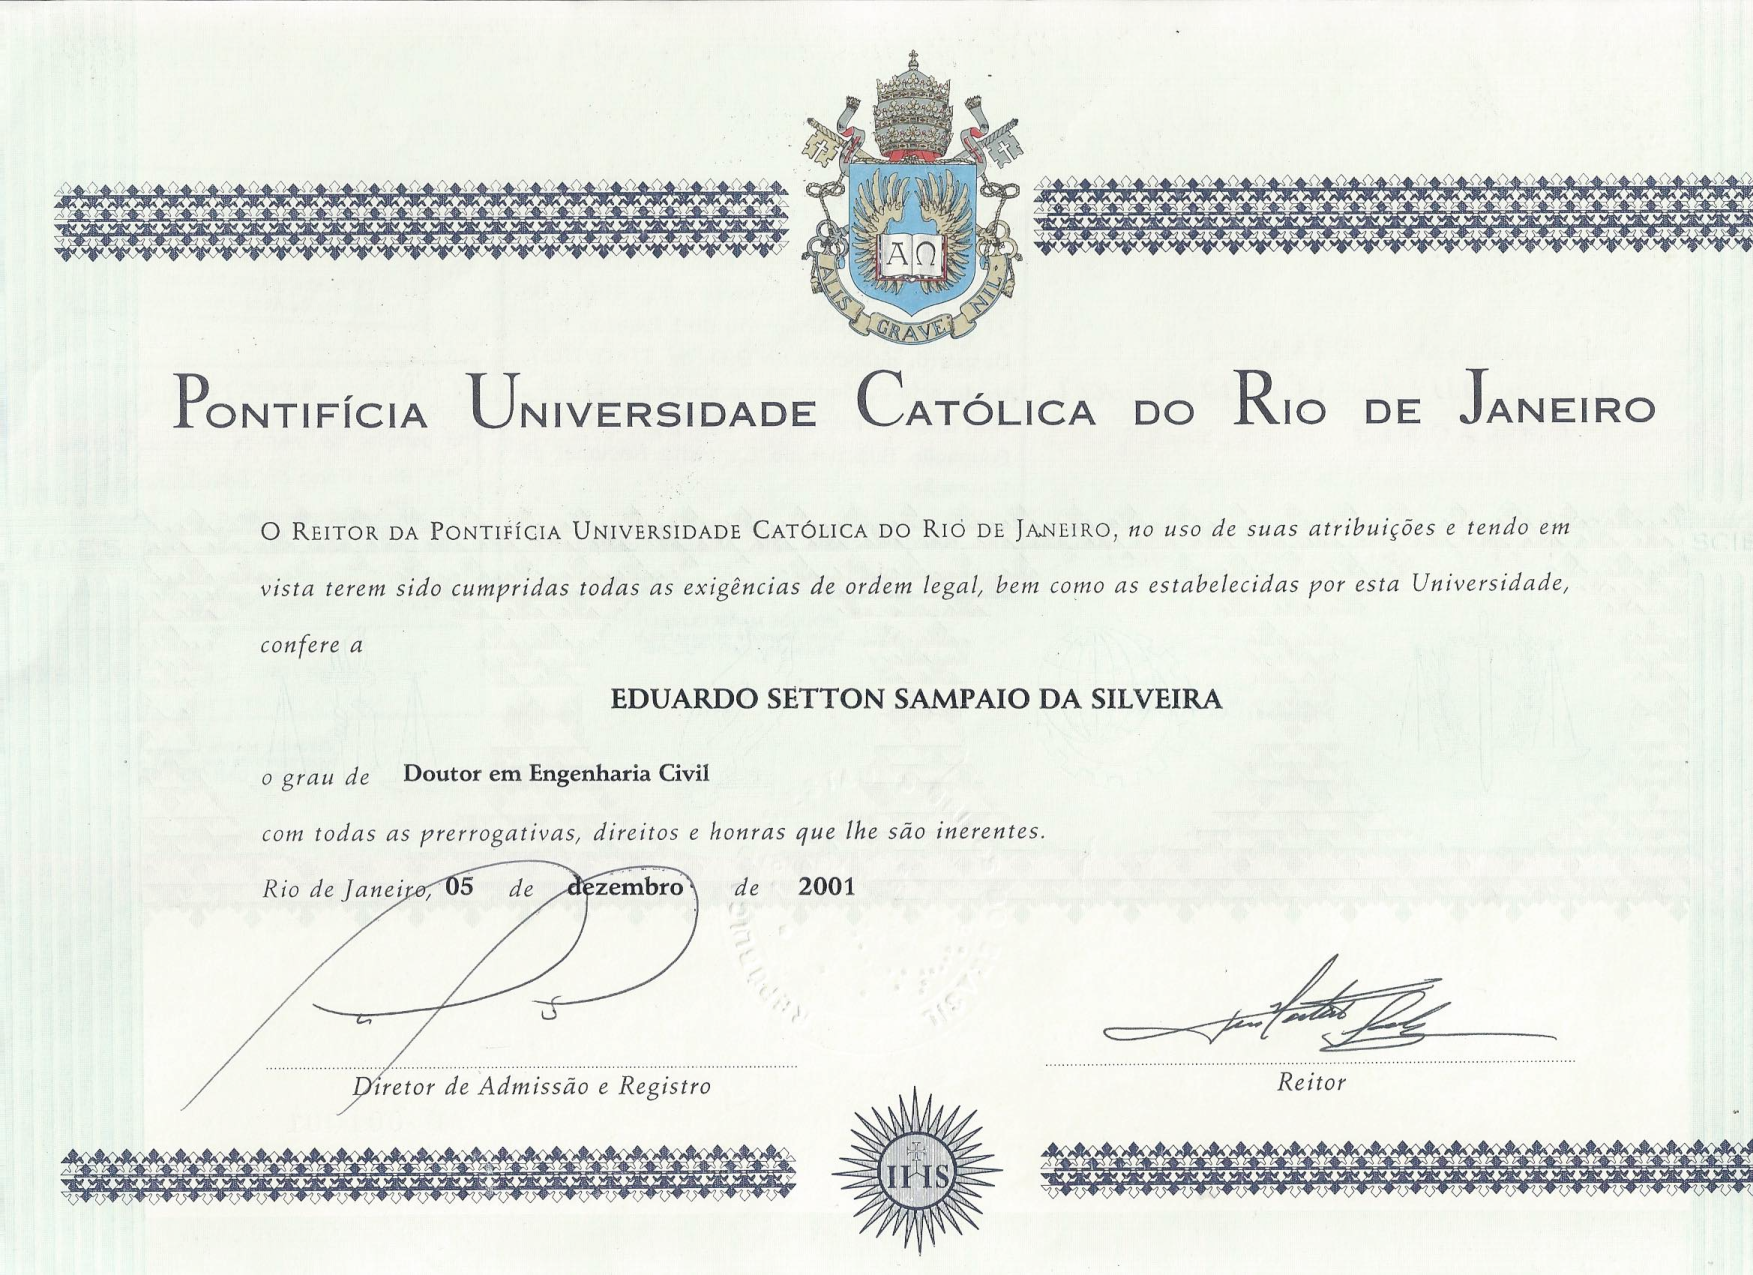
\includepdf[pages=-, scale=1,pagecommand=\thispagestyle{empty}]{\detokenize{GRUPO 1/Sub-Grupo 11/diplomadoutorado}}

\newpage
\subsection{Portaria Associado IV}
\label{portaria:associadoiv}
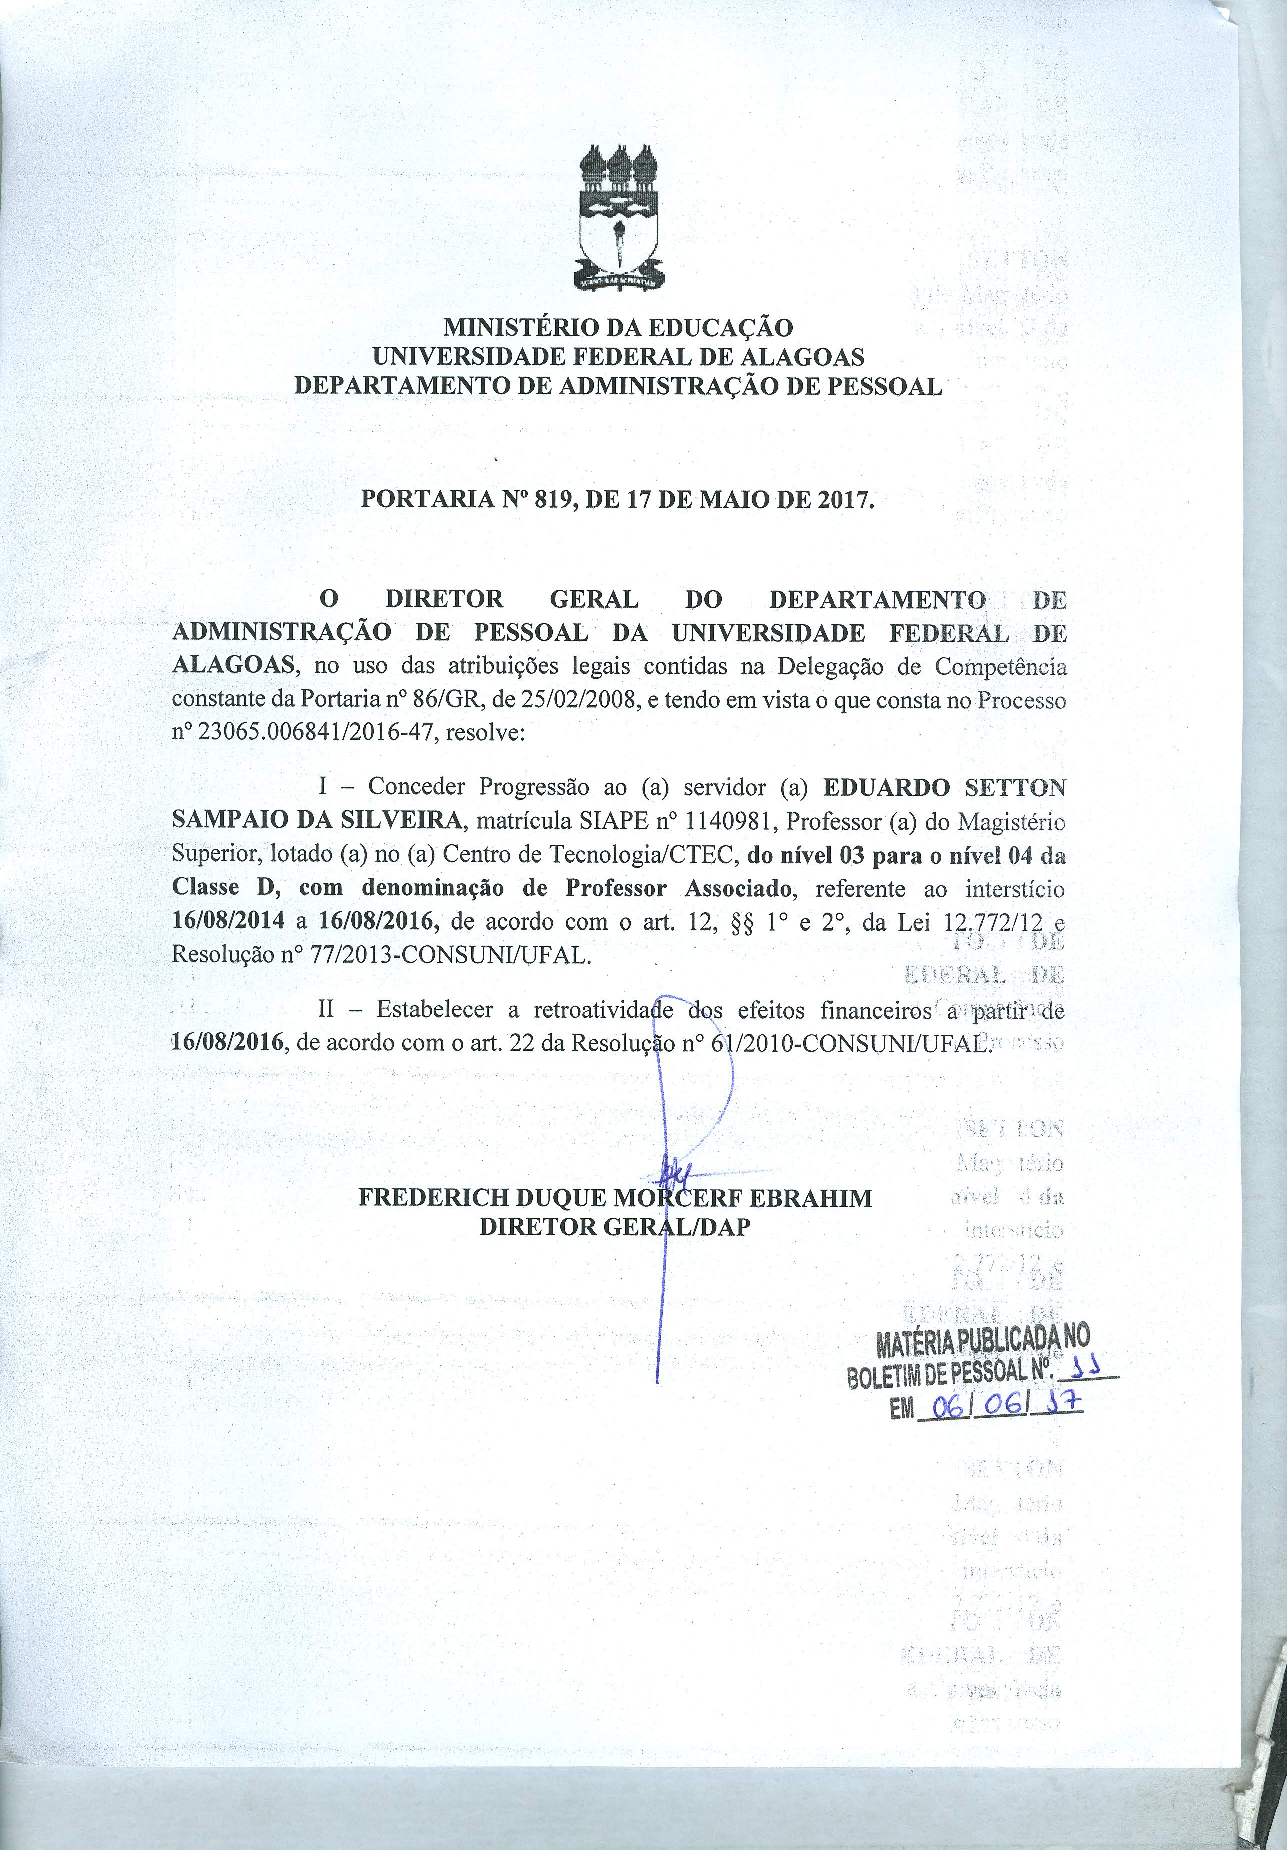
\includepdf[pages=-, scale=1,pagecommand=\thispagestyle{empty}]{\detokenize{GRUPO 1/Sub-Grupo 11/portariaufal1}}
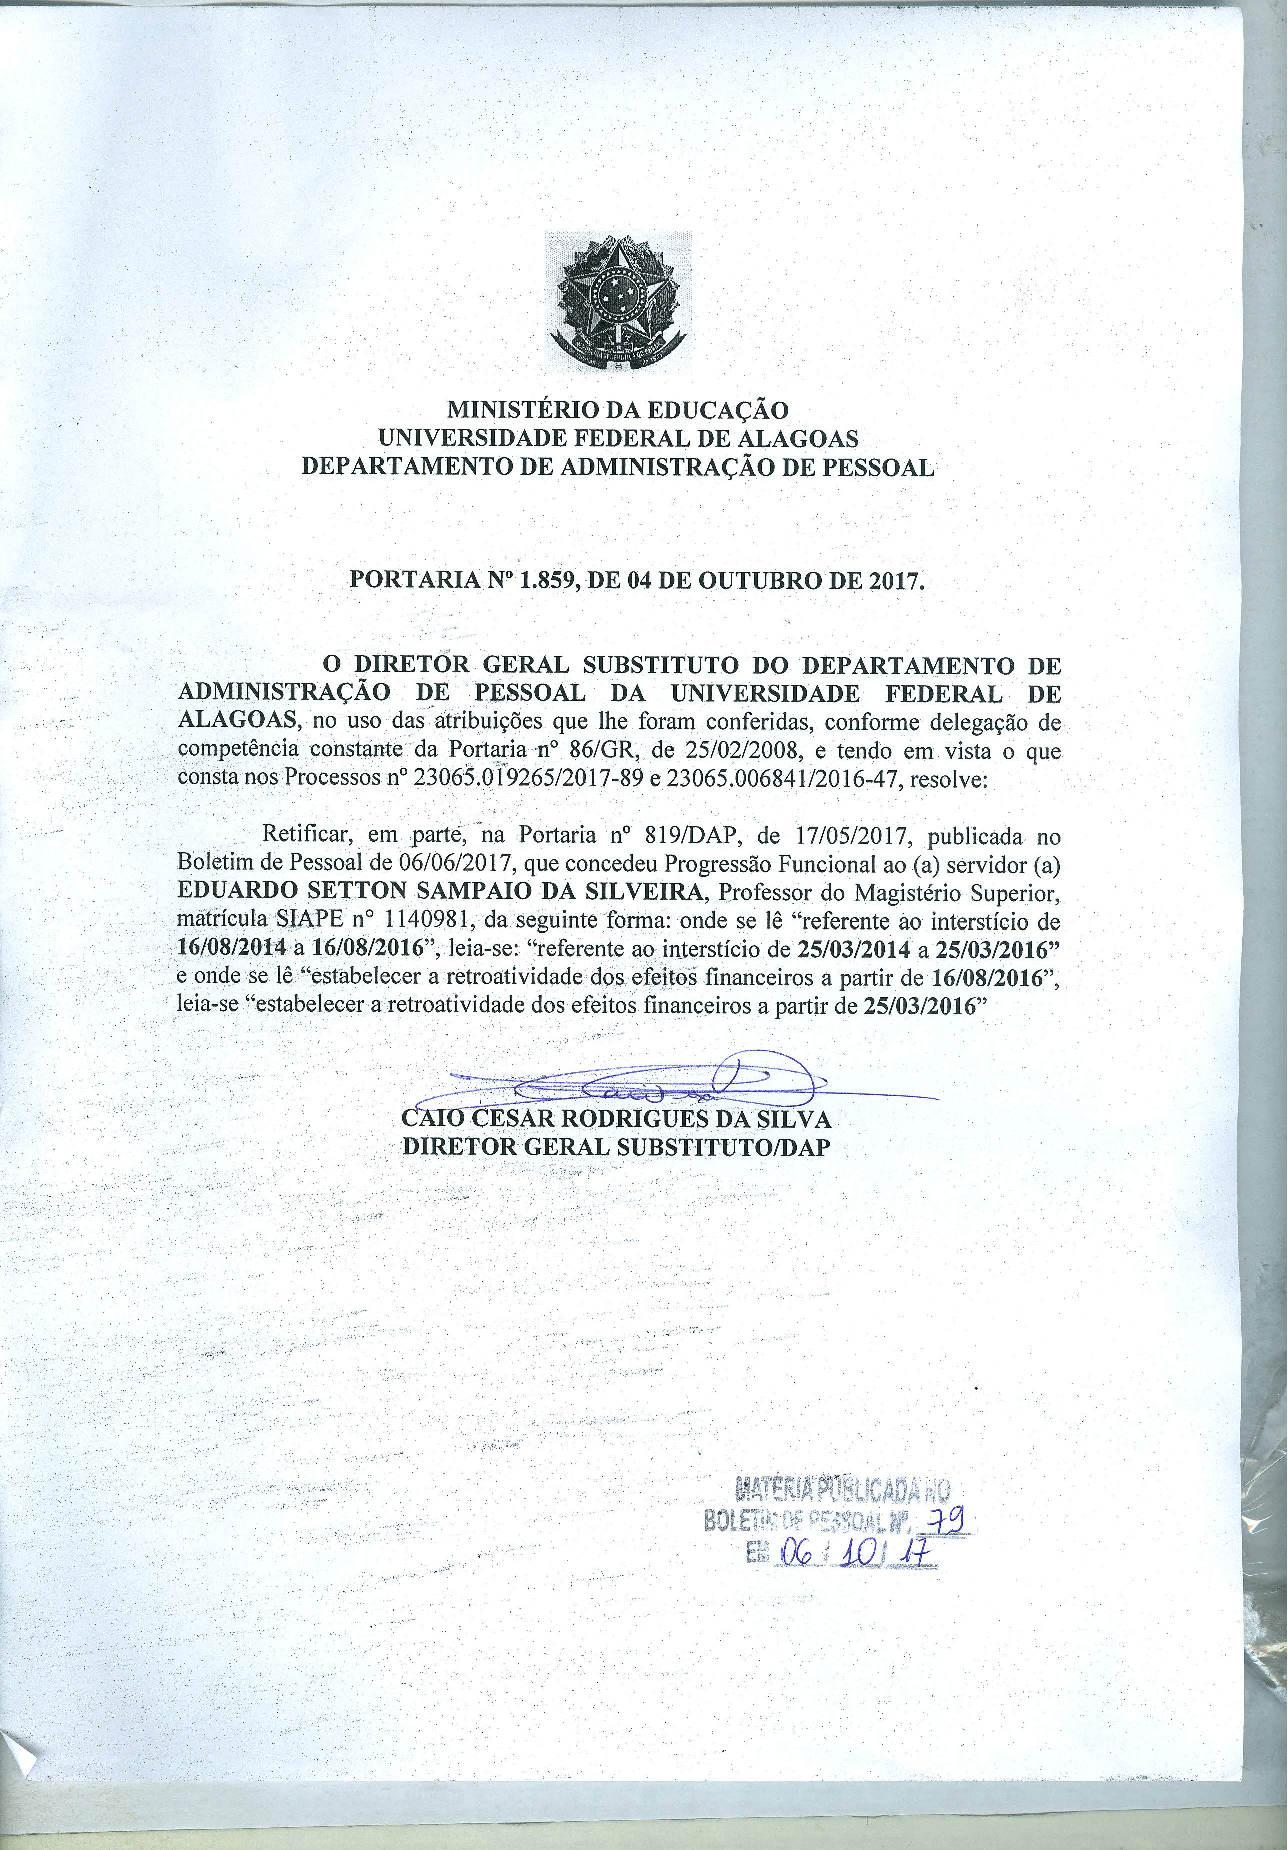
\includepdf[pages=-, scale=1,pagecommand=\thispagestyle{empty}]{\detokenize{GRUPO 1/Sub-Grupo 11/portariaufal2}}

%%%%%%%%%%%%%%%%%%%%%%%%%%%%%%%%%%%%%%%%%%%%%%%%%%%%%%%%%%%%%%%%%%%%%%%%%%%%%%%
% Grupo 1 - Atividades de Ensino
%%%%%%%%%%%%%%%%%%%%%%%%%%%%%%%%%%%%%%%%%%%%%%%%%%%%%%%%%%%%%%%%%%%%%%%%%%%%%%%

%%%%%%%%%%%%%%%%%%%%%%%%%%%%%%%%%%%%%%%%%%%%%%%%%%%%%%%%%%%%%%%%%%%%%%%%%%%%%%%
% Subgrupo 1.1 - Ministracão de Disciplinas
%%%%%%%%%%%%%%%%%%%%%%%%%%%%%%%%%%%%%%%%%%%%%%%%%%%%%%%%%%%%%%%%%%%%%%%%%%%%%%%
\newpage
\subsection{Disciplinas Ministradas}
\label{disciplinas:doc1}
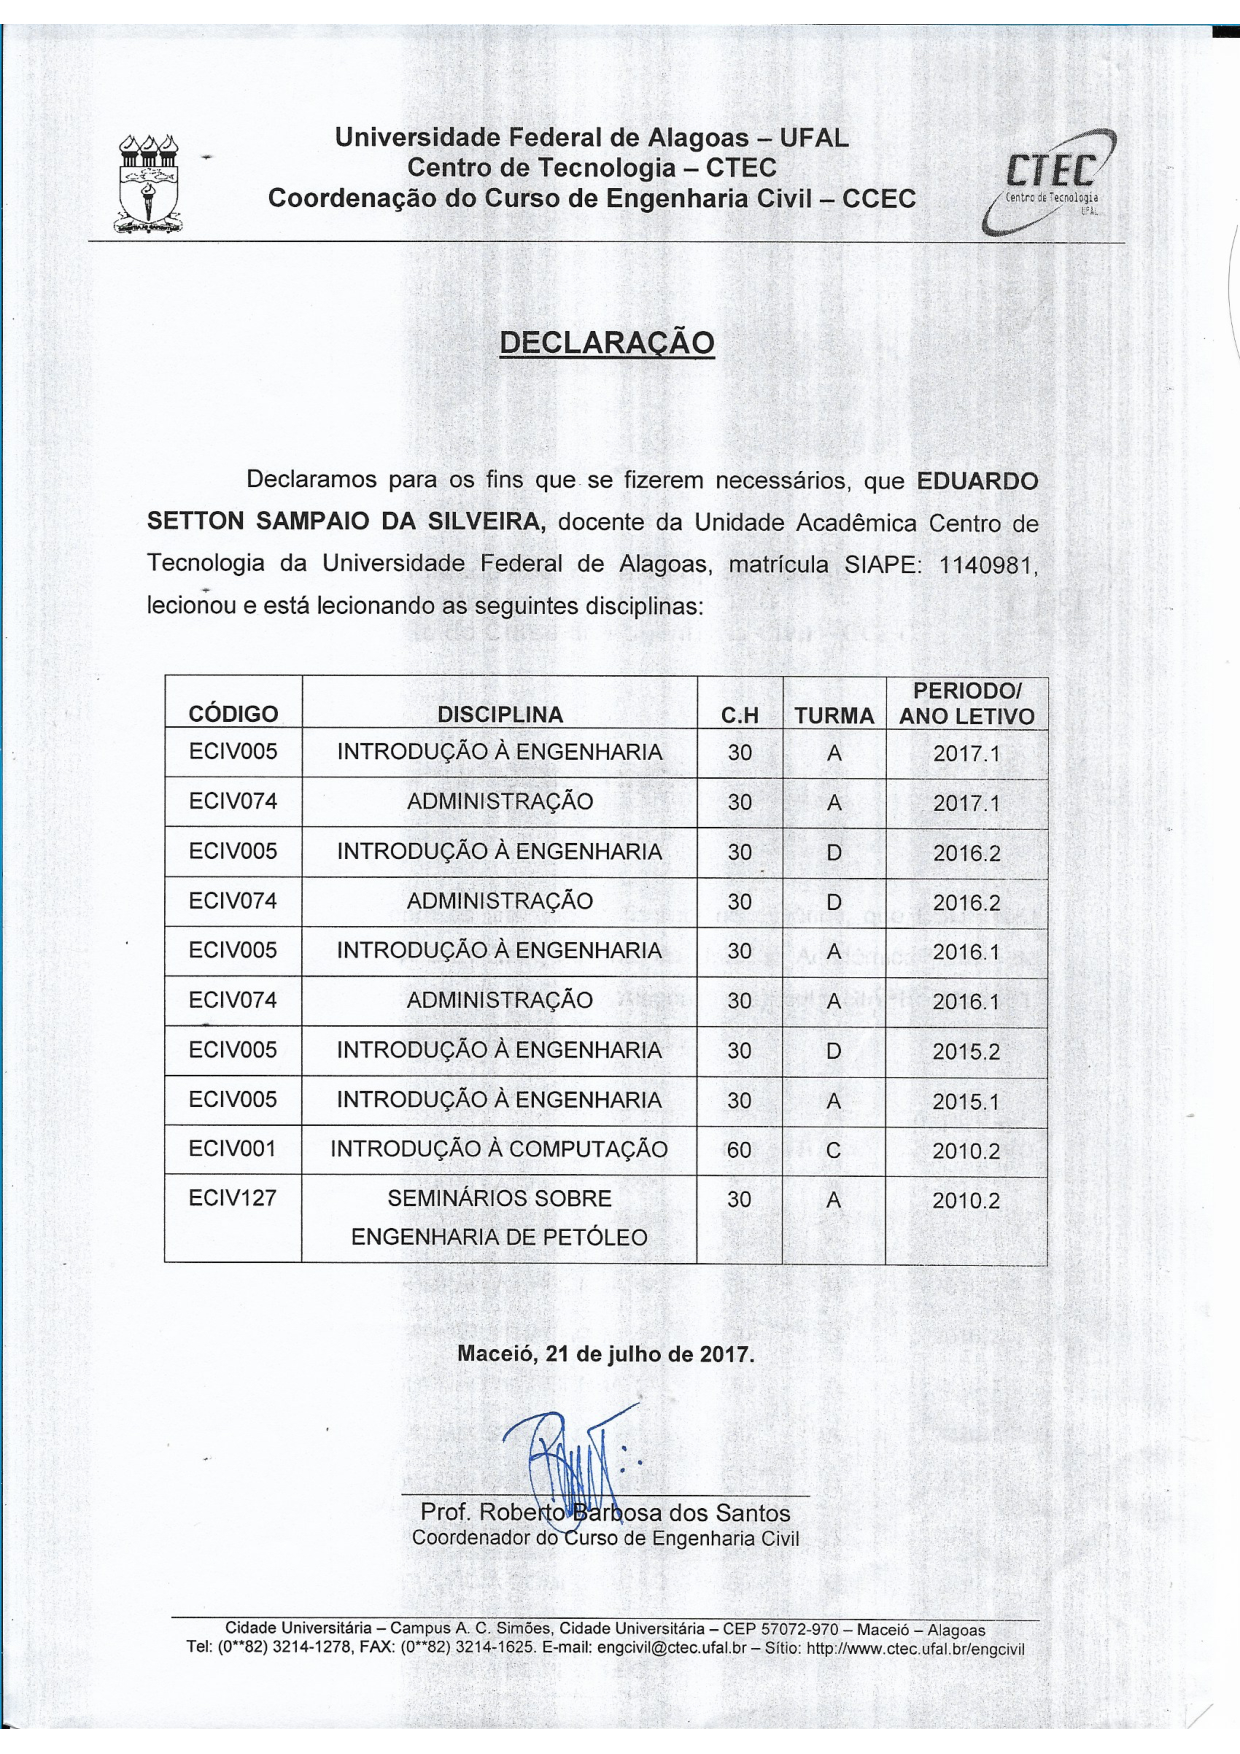
\includepdf[pages=-, scale=1,pagecommand=\thispagestyle{empty}]{\detokenize{GRUPO 1/Sub-Grupo 11/doc1}}

\newpage
\subsection{Disciplinas Ministradas}
\label{disciplinas:doc2}
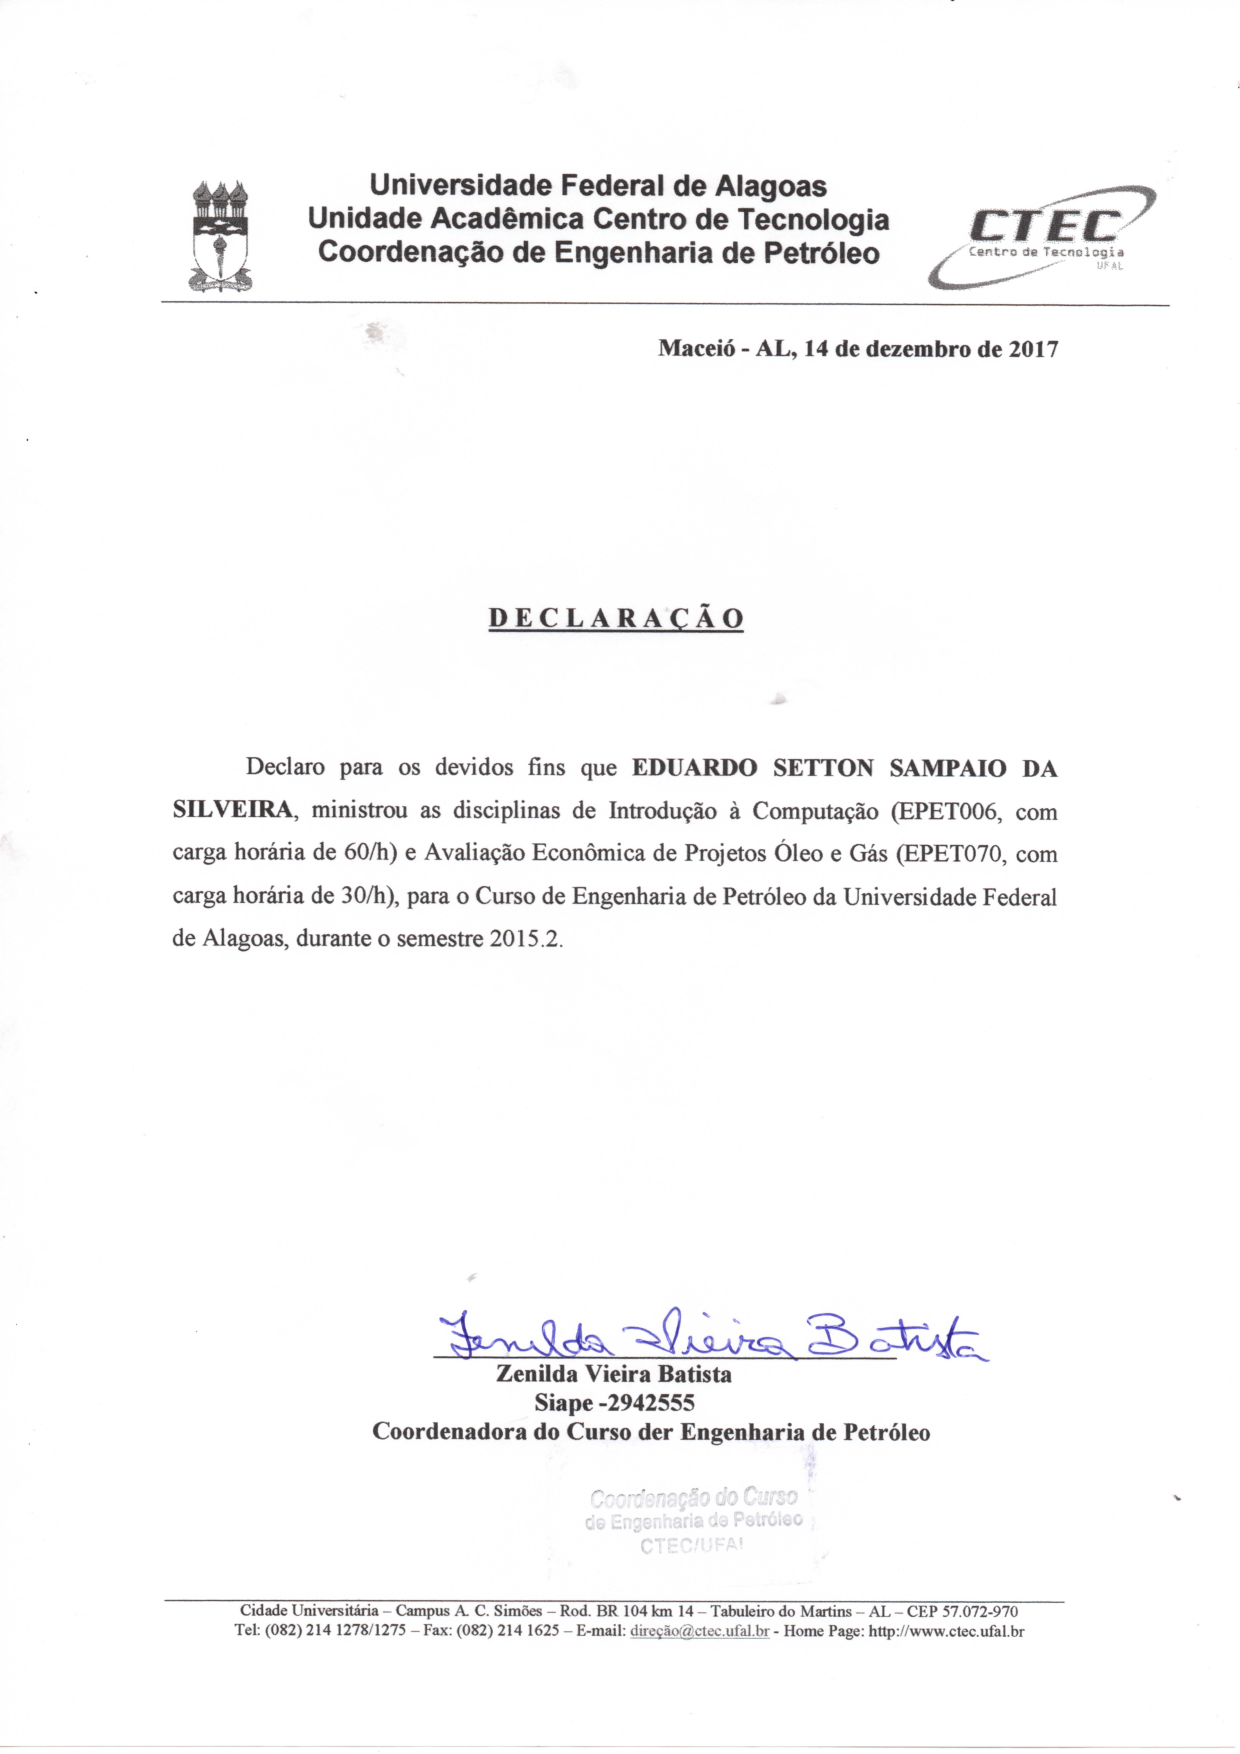
\includepdf[pages=-, scale=1,pagecommand=\thispagestyle{empty}]{\detokenize{GRUPO 1/Sub-Grupo 11/doc2}}

\newpage
\subsection{Disciplinas Ministradas}
\label{disciplinas:doc3}
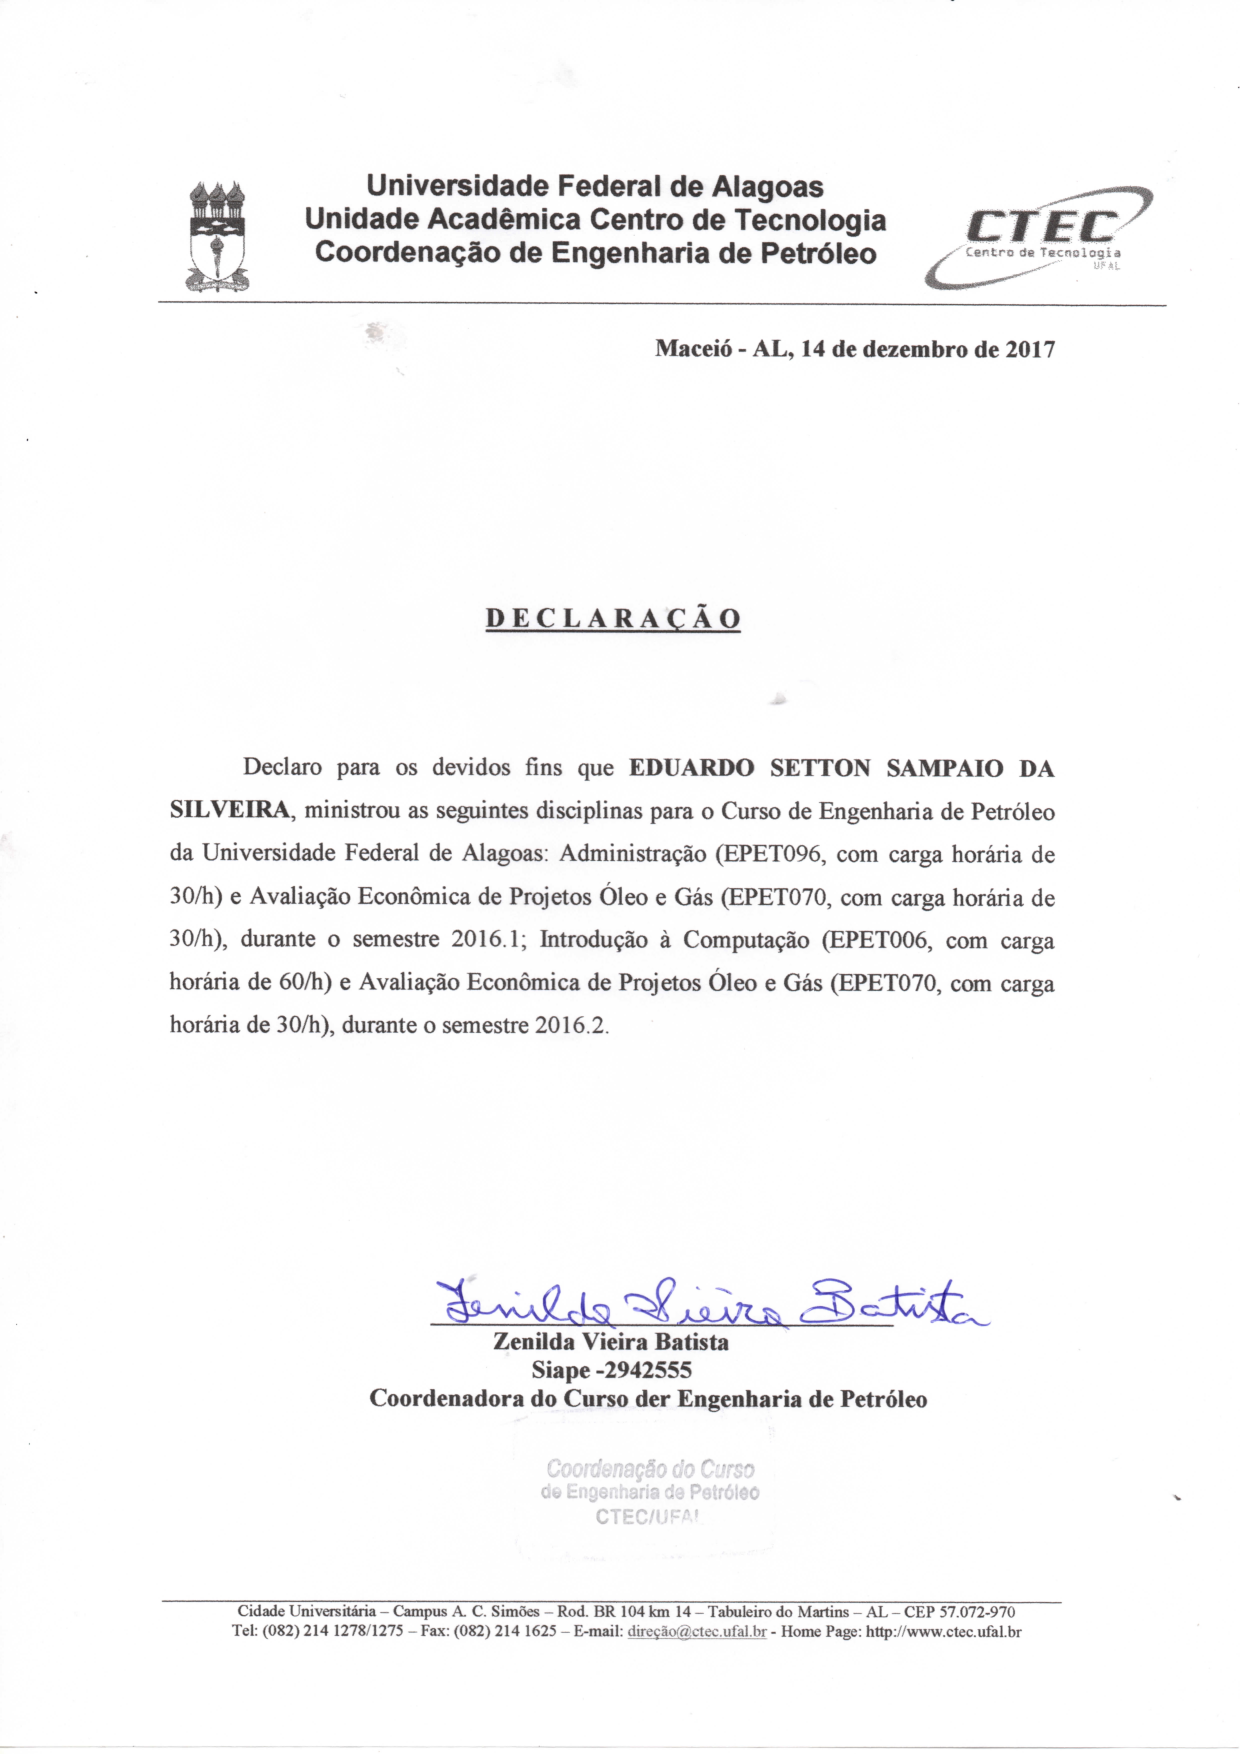
\includepdf[pages=-, scale=1,pagecommand=\thispagestyle{empty}]{\detokenize{GRUPO 1/Sub-Grupo 11/doc3}}

\newpage
\subsection{Disciplinas Ministradas}
\label{disciplinas:doc4}
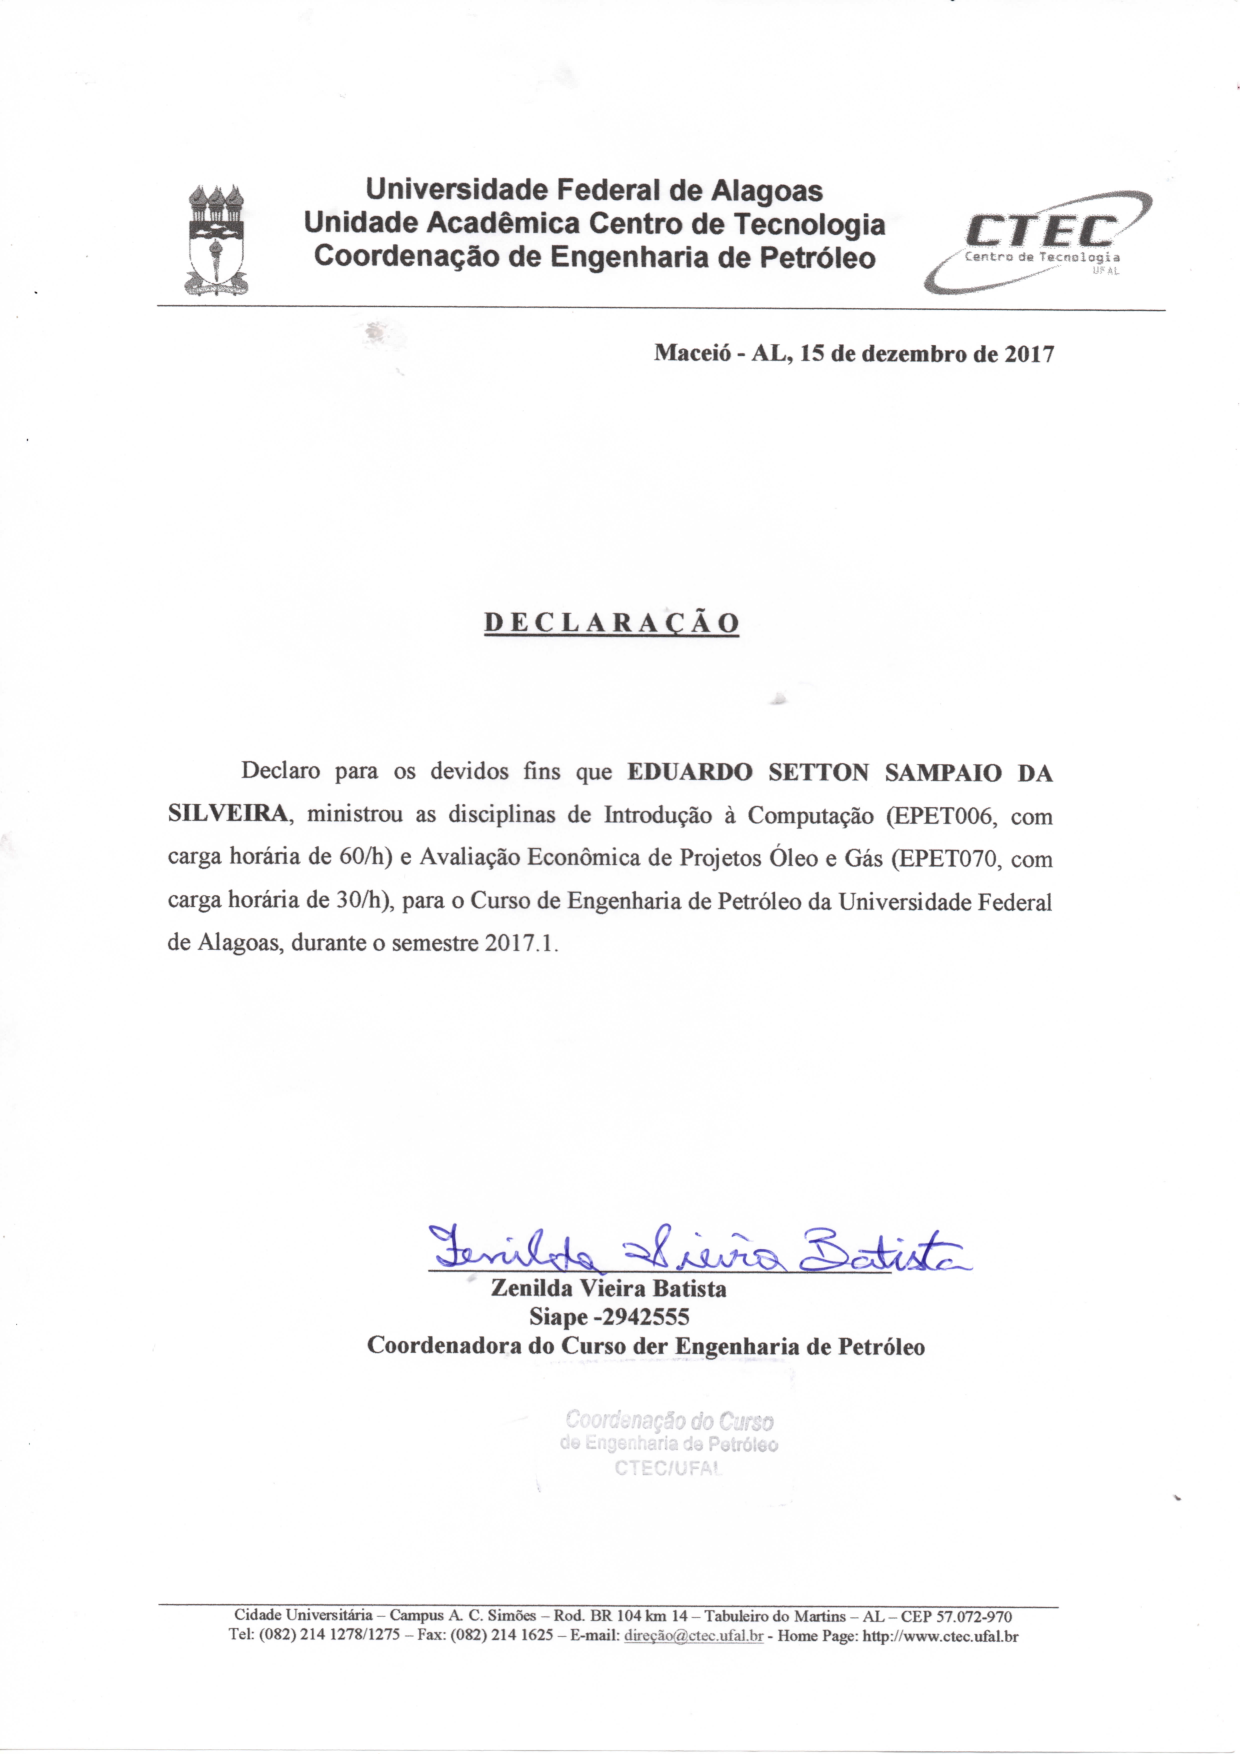
\includepdf[pages=-, scale=1,pagecommand=\thispagestyle{empty}]{\detokenize{GRUPO 1/Sub-Grupo 11/doc4}}

\newpage
\subsection{Disciplinas Ministradas}
\label{disciplinas:doc5}
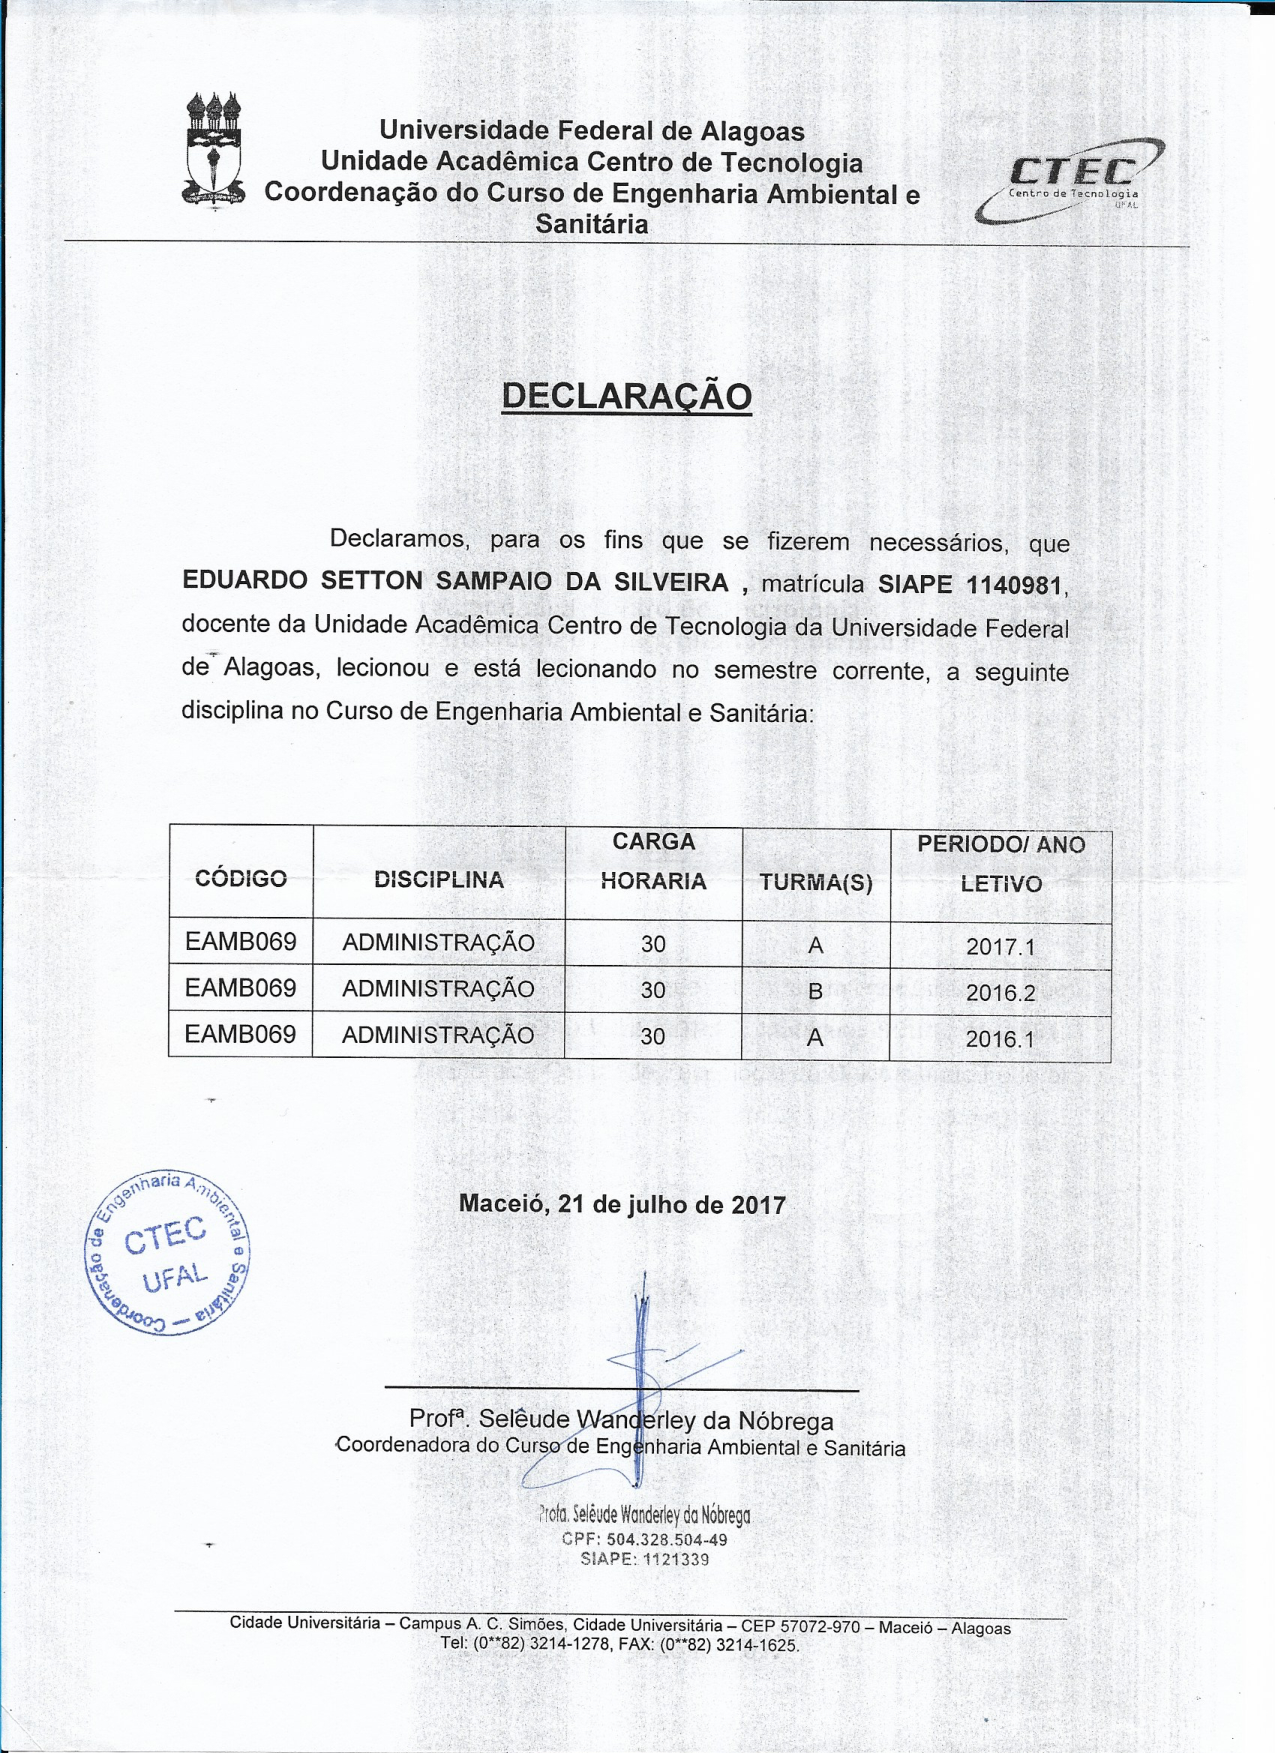
\includepdf[pages=-, scale=1,pagecommand=\thispagestyle{empty}]{\detokenize{GRUPO 1/Sub-Grupo 11/doc5}}

\newpage
\subsection{Disciplinas Ministradas}
\label{disciplinas:doc6profnit}
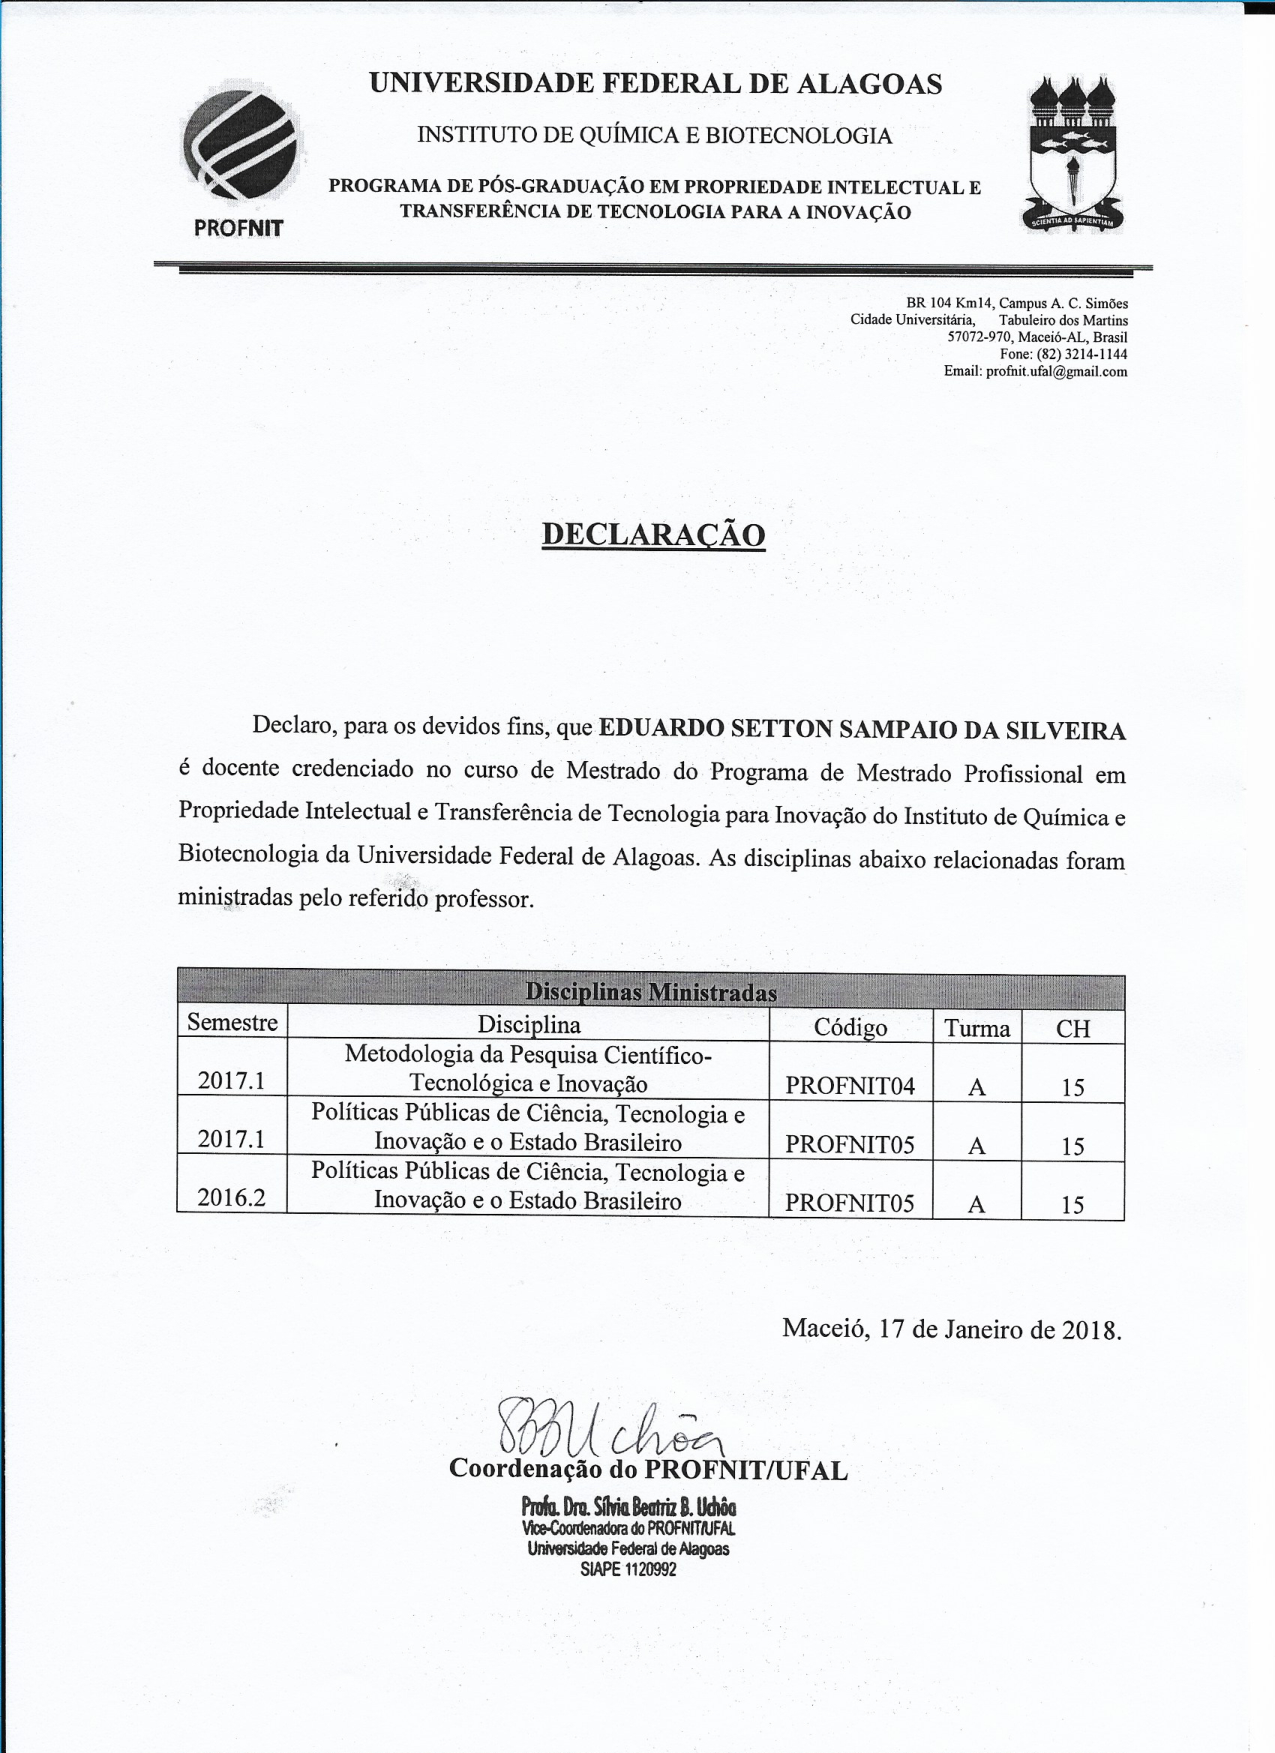
\includepdf[pages=-, scale=1,pagecommand=\thispagestyle{empty}]{\detokenize{GRUPO 1/Sub-Grupo 11/doc6profinit}}

%%%%%%%%%%%%%%%%%%%%%%%%%%%%%%%%%%%%%%%%%%%%%%%%%%%%%%%%%%%%%%%%%%%%%%%%%%%%%%%
% Subgrupo 1.2 - Orientações
%%%%%%%%%%%%%%%%%%%%%%%%%%%%%%%%%%%%%%%%%%%%%%%%%%%%%%%%%%%%%%%%%%%%%%%%%%%%%%%

\newpage
\subsection{Orientações de Trabalhos de Conclusão de Curso Concluídas}
\label{tcc:doc7}
Esta subseção apresenta o comprovante das orientações de Trabalhos de Conclusão de Curso concluídos.
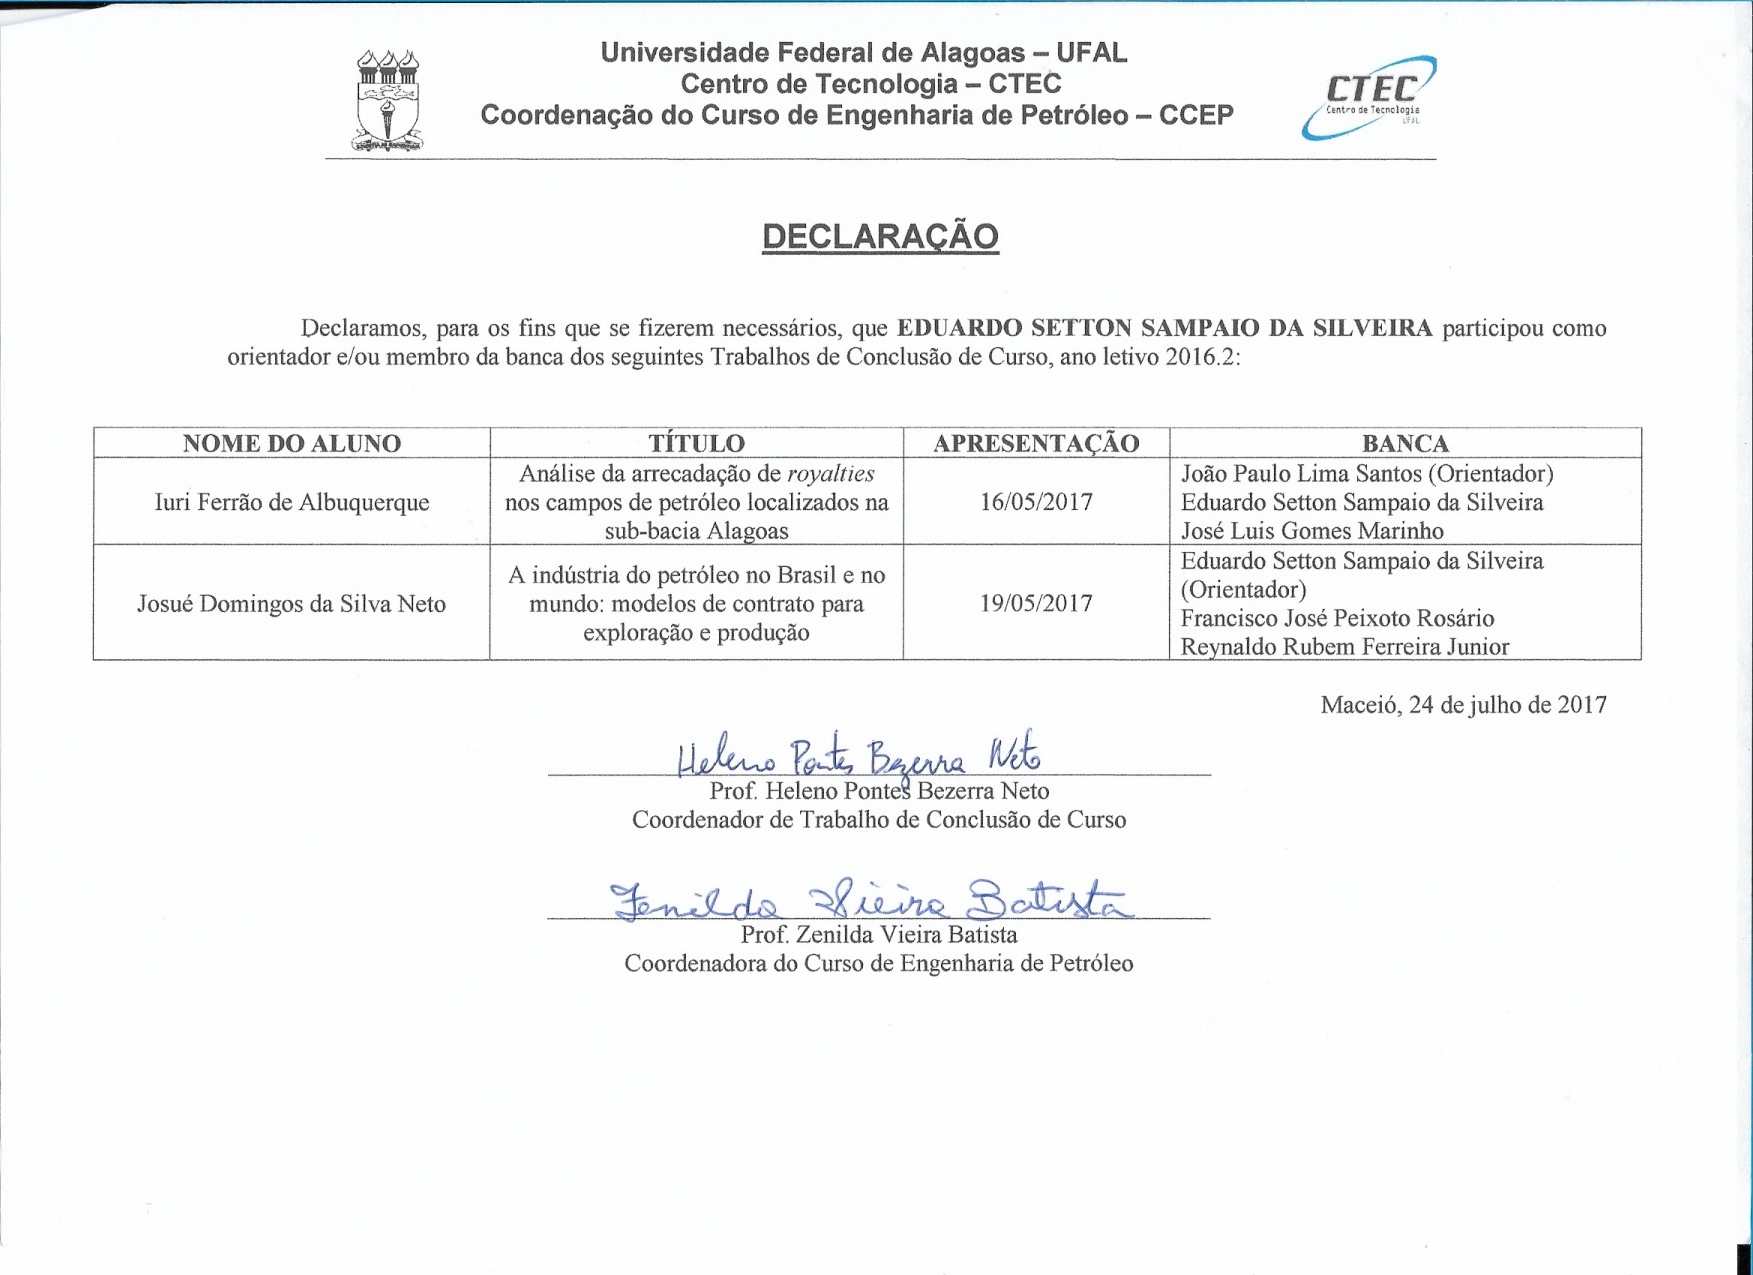
\includepdf[pages=-, scale=1,pagecommand=\thispagestyle{empty}]{\detokenize{GRUPO 1/Sub-Grupo 12/doc7}}

\newpage
\subsection{Orientações de Trabalhos de Conclusão de Curso Concluídas}
\label{tcc:doc8}
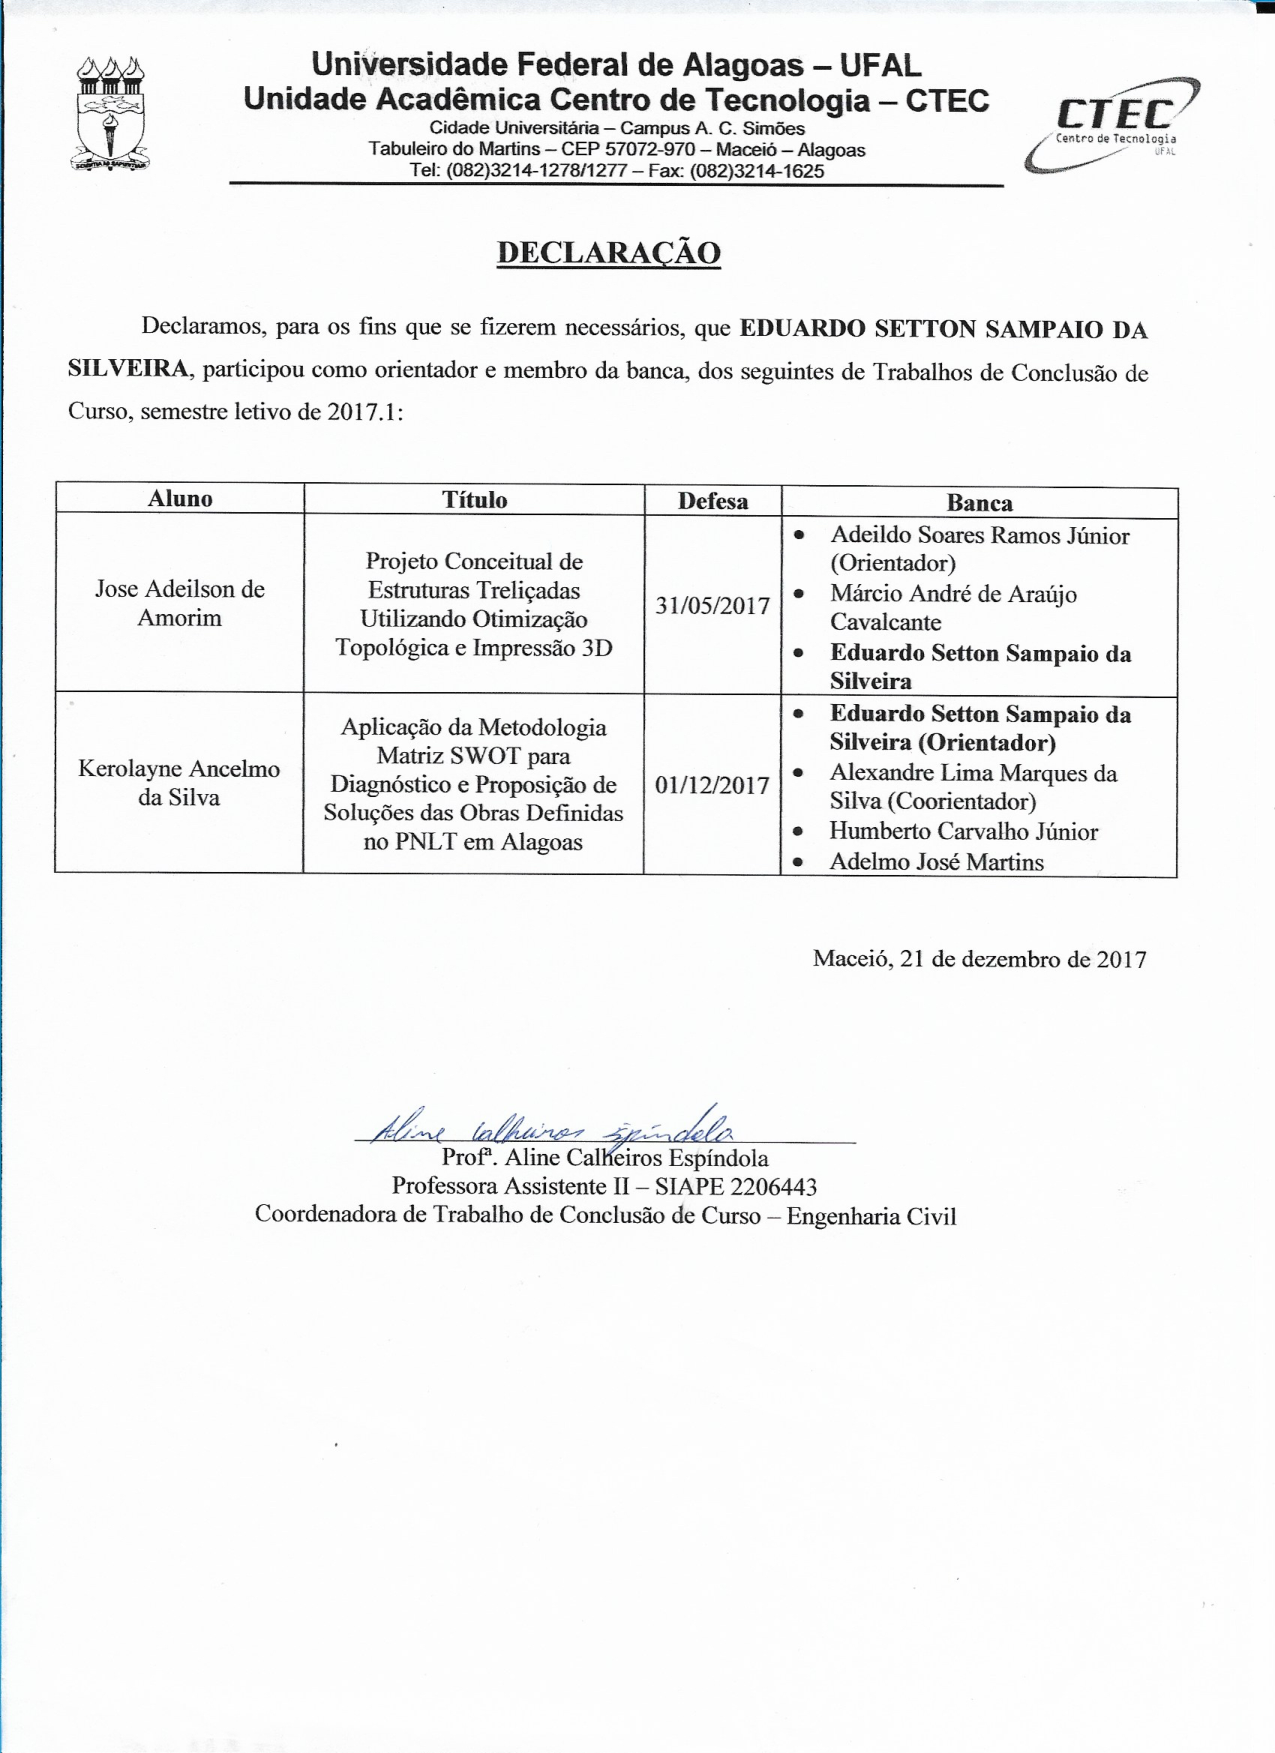
\includepdf[pages=-, scale=1,pagecommand=\thispagestyle{empty}]{\detokenize{GRUPO 1/Sub-Grupo 12/doc8}}

\newpage
\subsection{Supervisão direta de estágios curriculares}
\label{advisor:estagio}
Esta subseção apresenta o comprovante de supervisão de estágios curriculares.
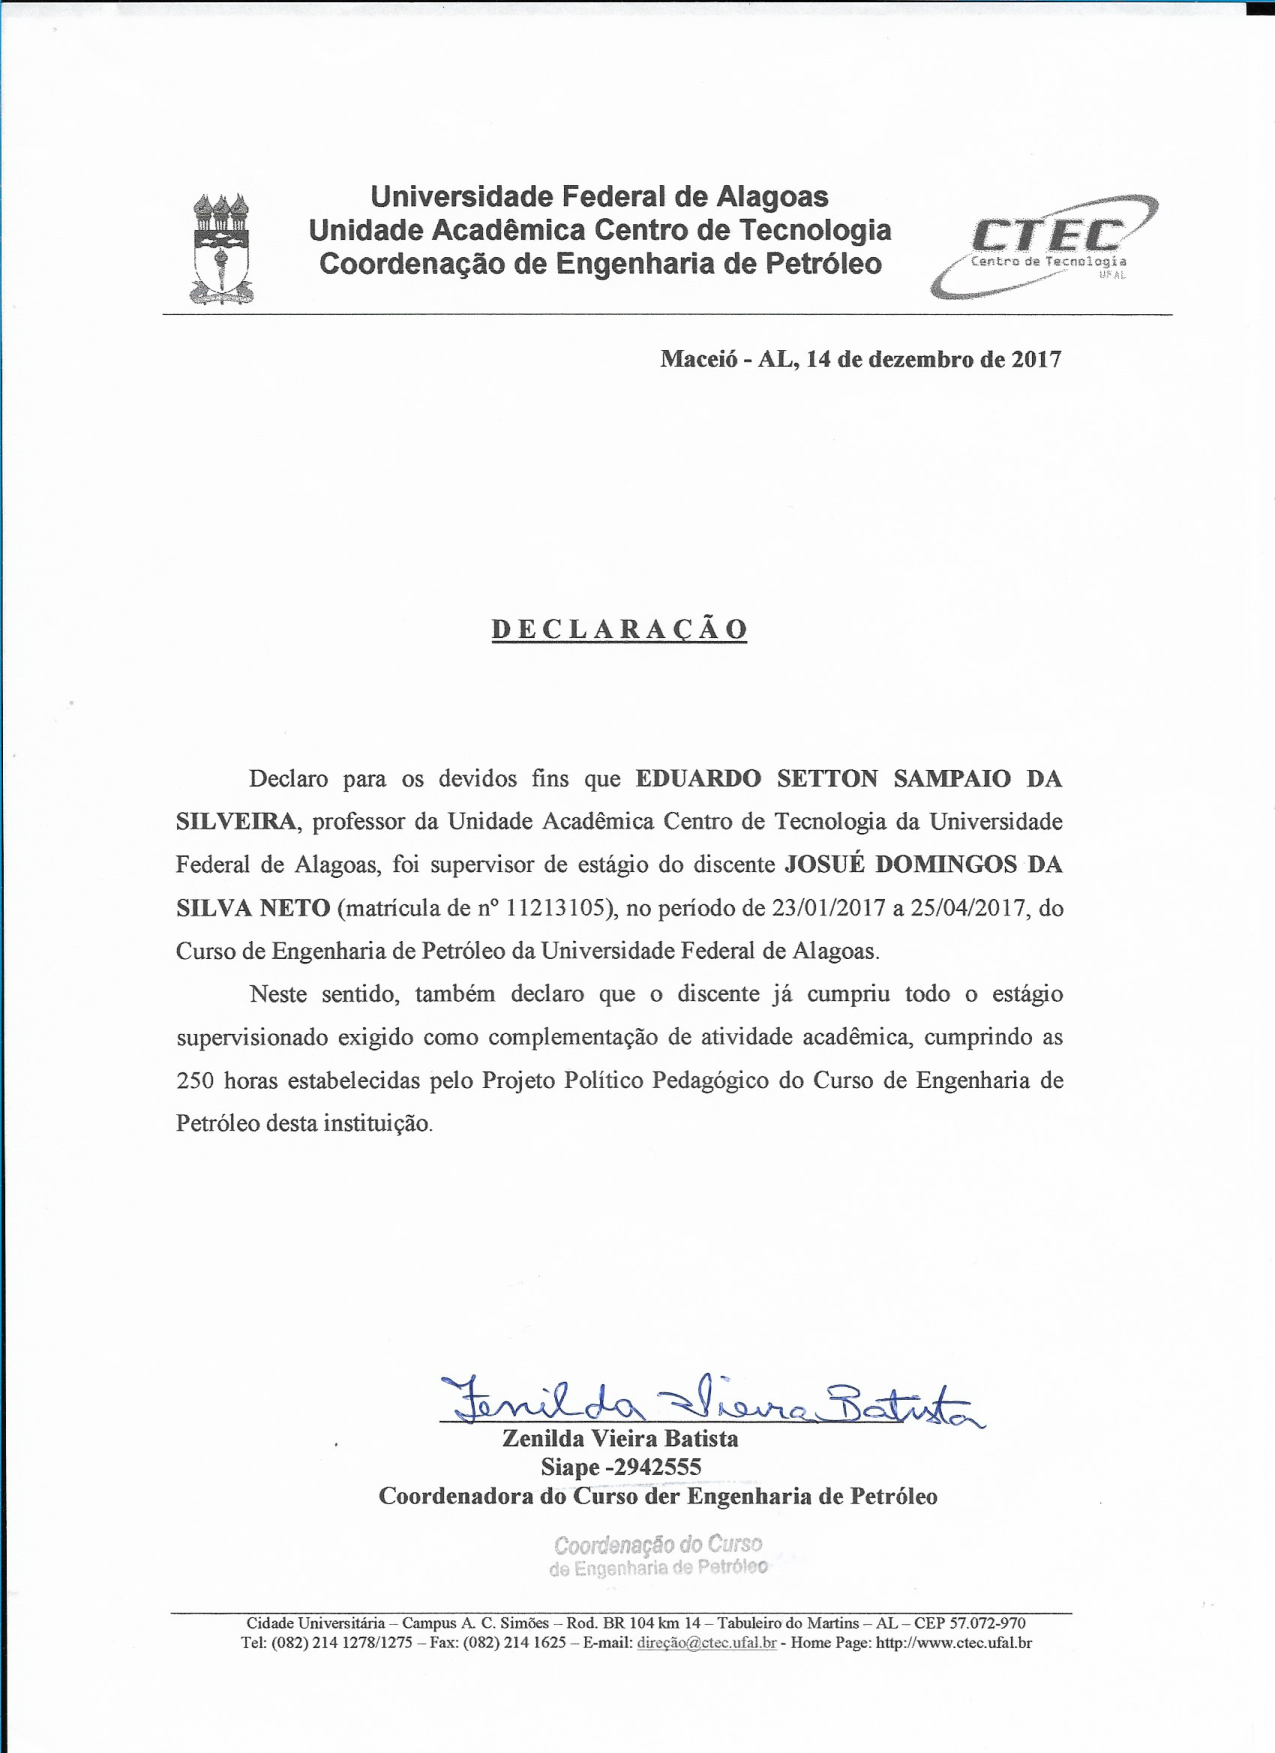
\includepdf[pages=-, scale=1,pagecommand=\thispagestyle{empty}]{\detokenize{GRUPO 1/Sub-Grupo 12/doc9}}

\newpage
\subsection{Supervisão e acompanhamento de monitorias}
\label{orient:monitoria1}
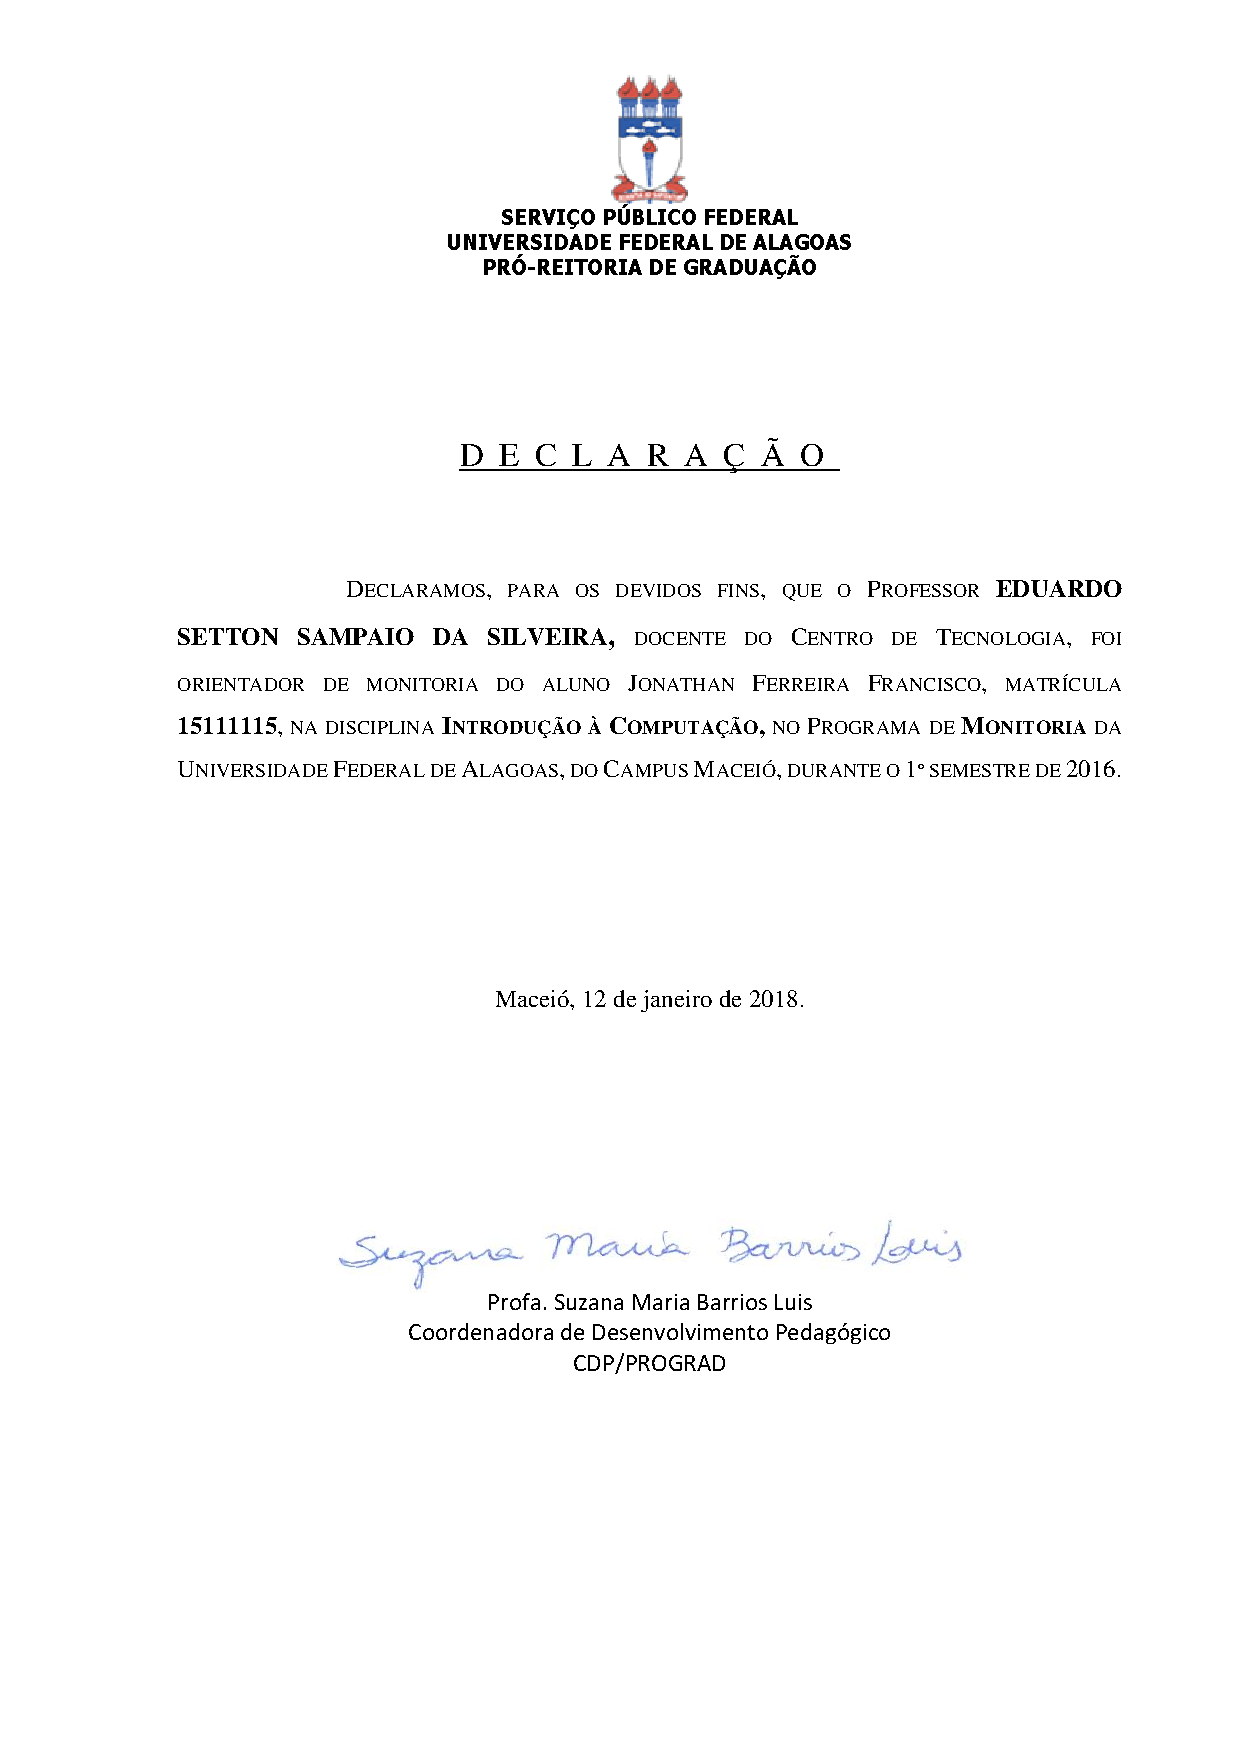
\includepdf[pages=-, scale=1,pagecommand=\thispagestyle{empty}]{\detokenize{GRUPO 1/Sub-Grupo 12/orient-monitoria1}}

\subsection{Supervisão e acompanhamento de monitorias}
\label{orient:monitoria2}
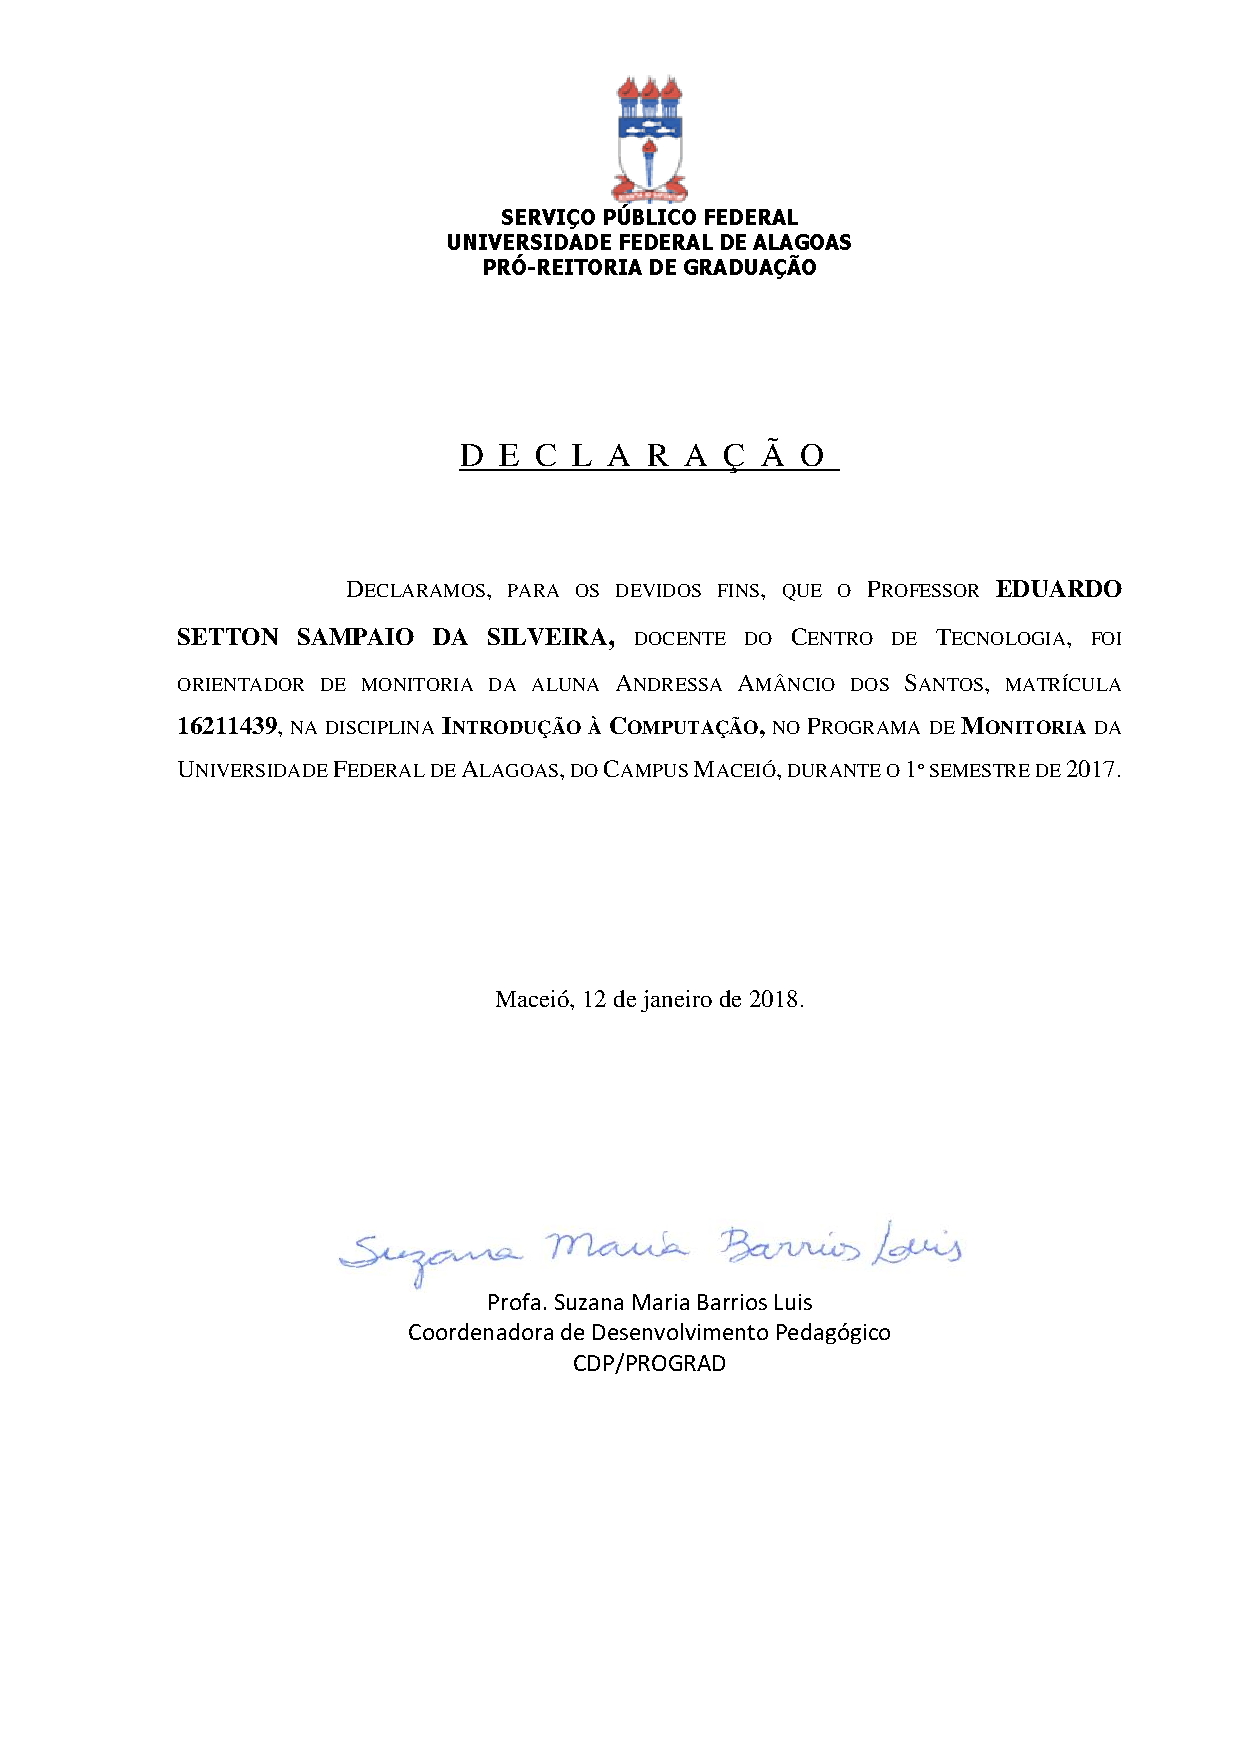
\includepdf[pages=-, scale=1,pagecommand=\thispagestyle{empty}]{\detokenize{GRUPO 1/Sub-Grupo 12/orient-monitoria2}}

\subsection{Supervisão e acompanhamento de monitorias}
\label{orient:monitoria3}
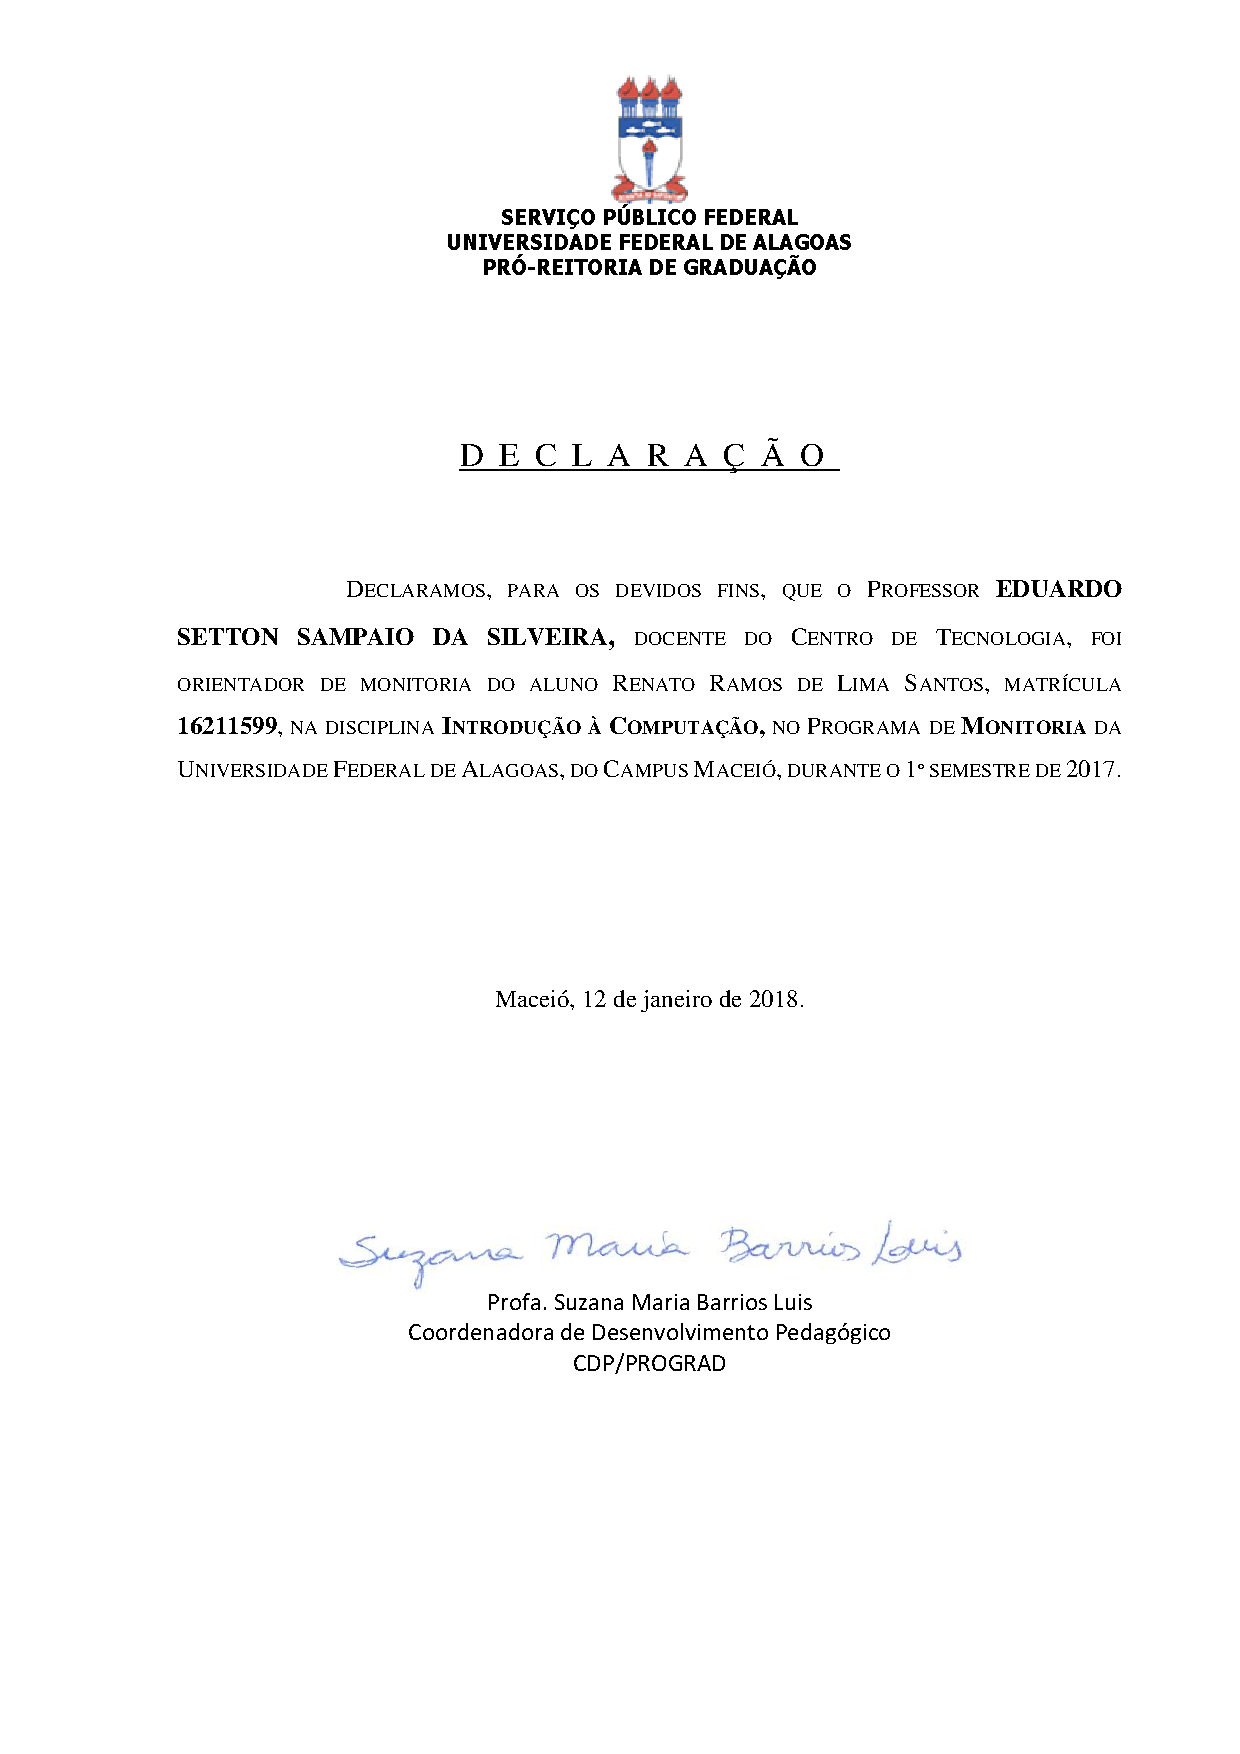
\includepdf[pages=-, scale=1,pagecommand=\thispagestyle{empty}]{\detokenize{GRUPO 1/Sub-Grupo 12/orient-monitoria3}}

\newpage
\subsection{Orientação de dissertação de Mestrado em andamento, por semestre}
\label{advisor:msc-andamento}
Esta subseção apresenta o comprovante de orientações de Dissertação de Mestrado em andamento.
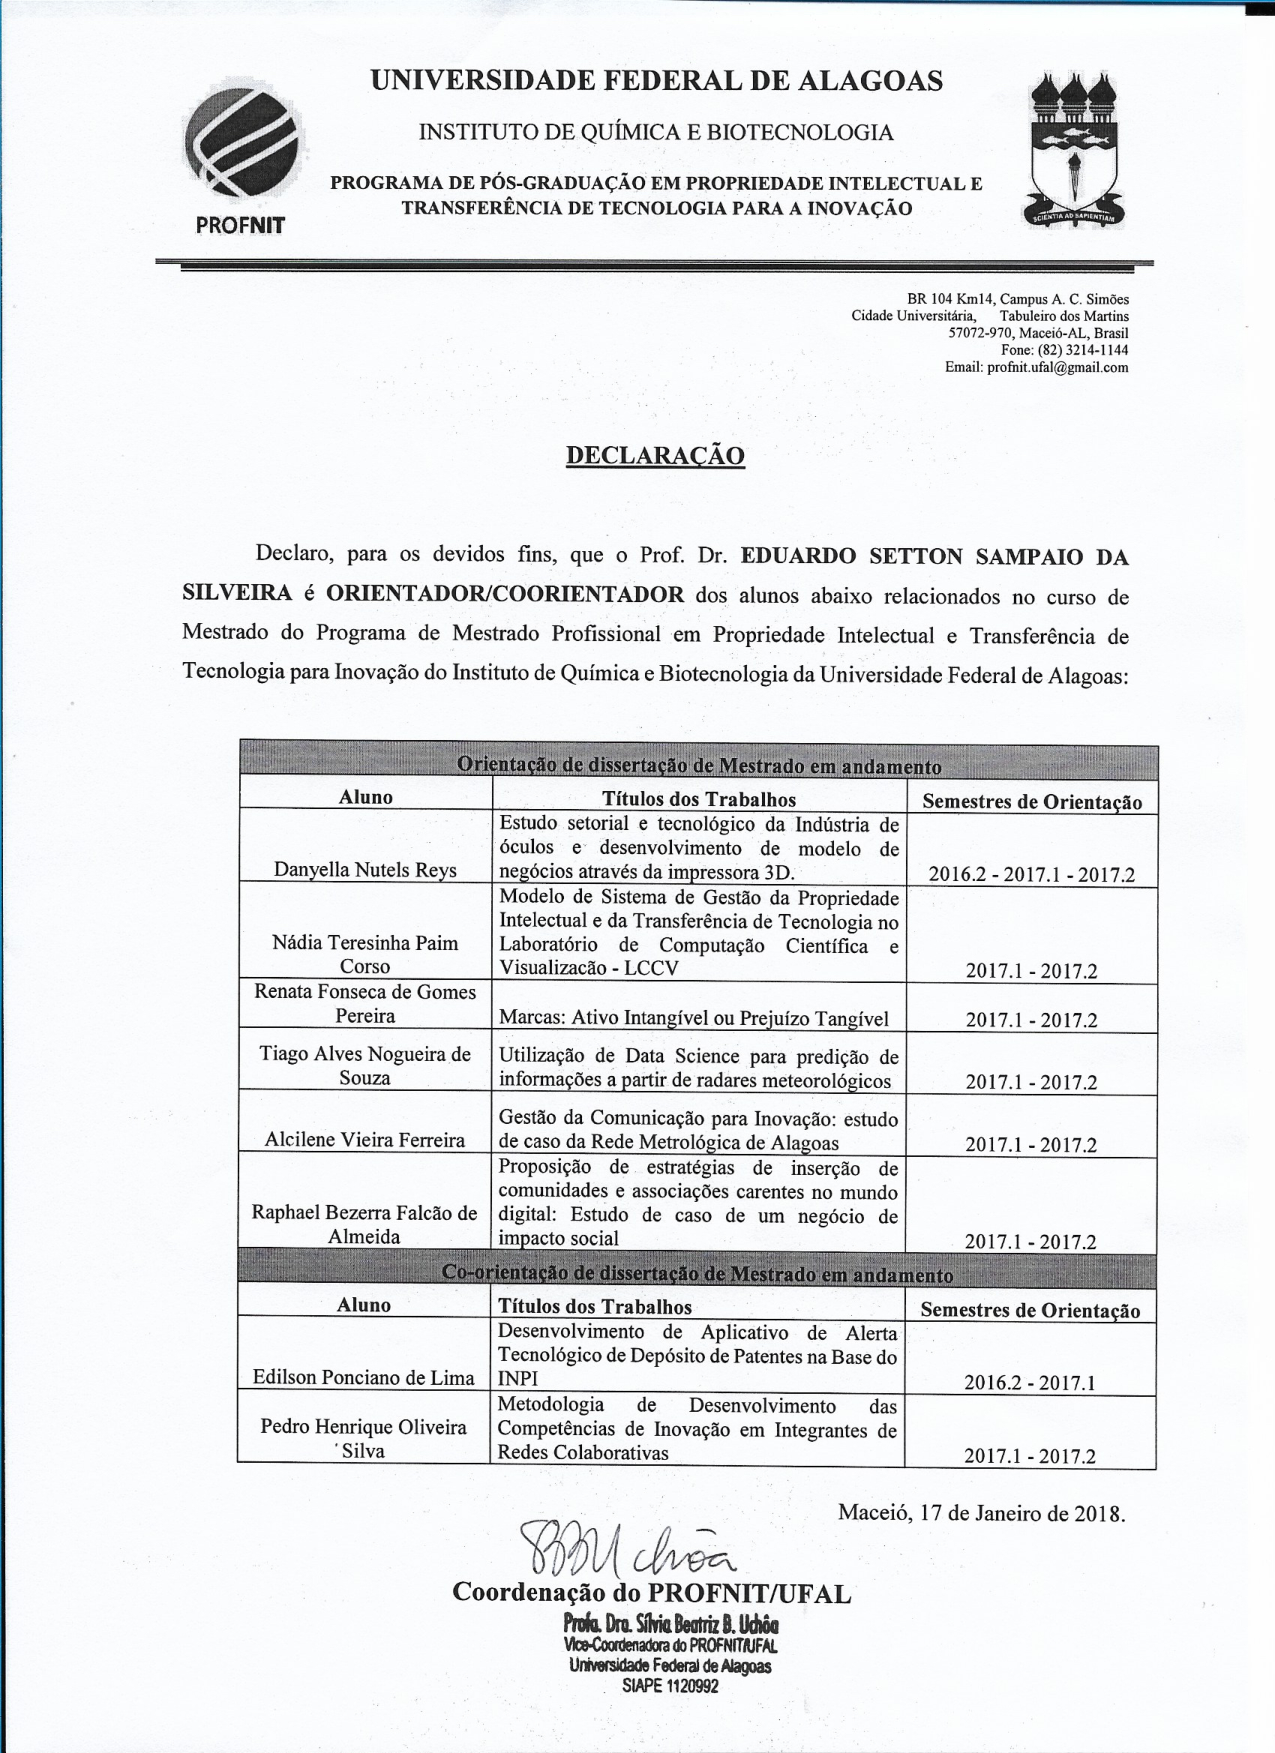
\includepdf[pages=-, scale=1,pagecommand=\thispagestyle{empty}]{\detokenize{GRUPO 1/Sub-Grupo 12/msc-andamento}}

\newpage
\subsection{Co-orientação de dissertação de Mestrado em andamento, por semestre}
\label{advisor:mscco-andamento}
Esta subseção apresenta o comprovante de co-orientações de Dissertação de Mestrado em andamento.
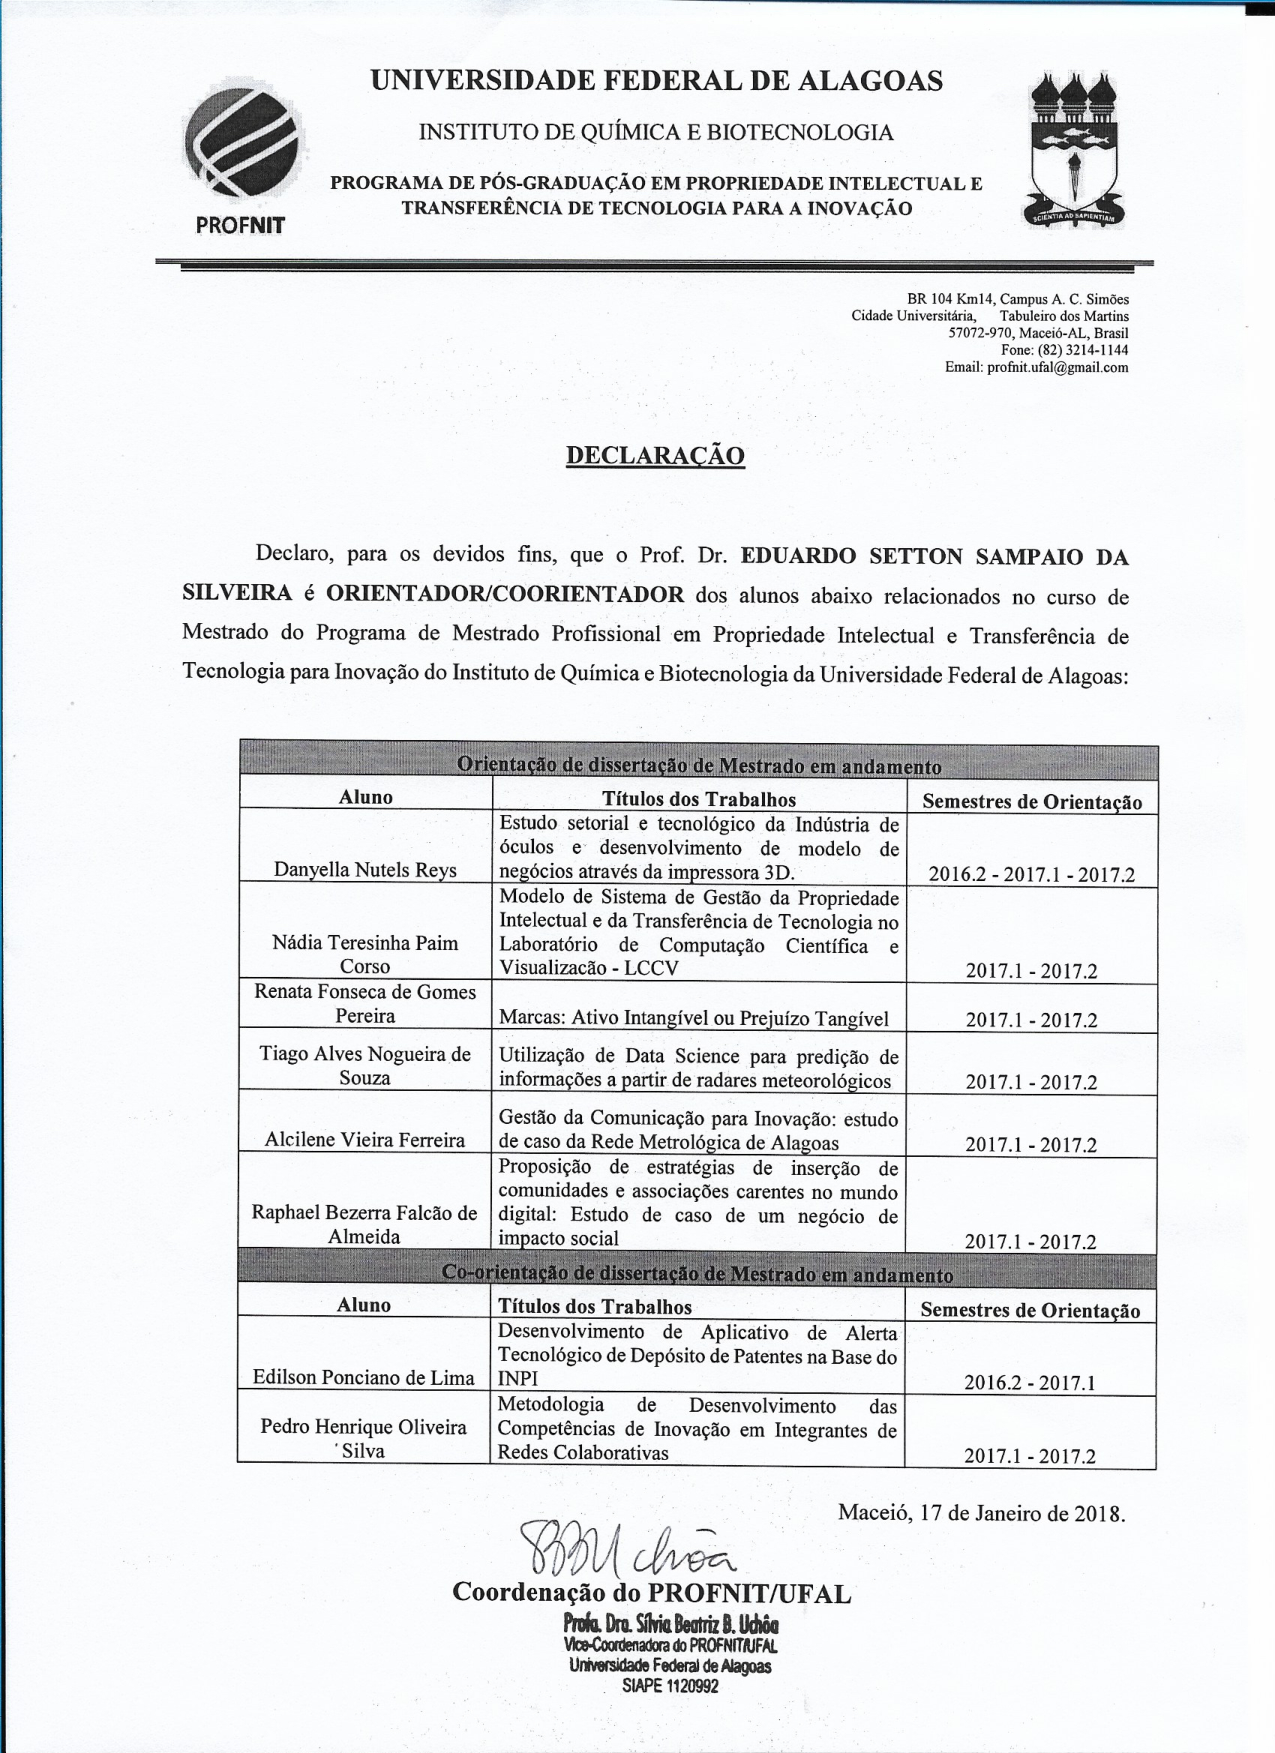
\includepdf[pages=-, scale=1,pagecommand=\thispagestyle{empty}]{\detokenize{GRUPO 1/Sub-Grupo 12/mscco-andamento}}

\newpage
\subsection{Orientação de estudantes de graduação em programas institucionalizados de pesquisa em andamento, por semestre}
\label{advisor:ict-lccv1}
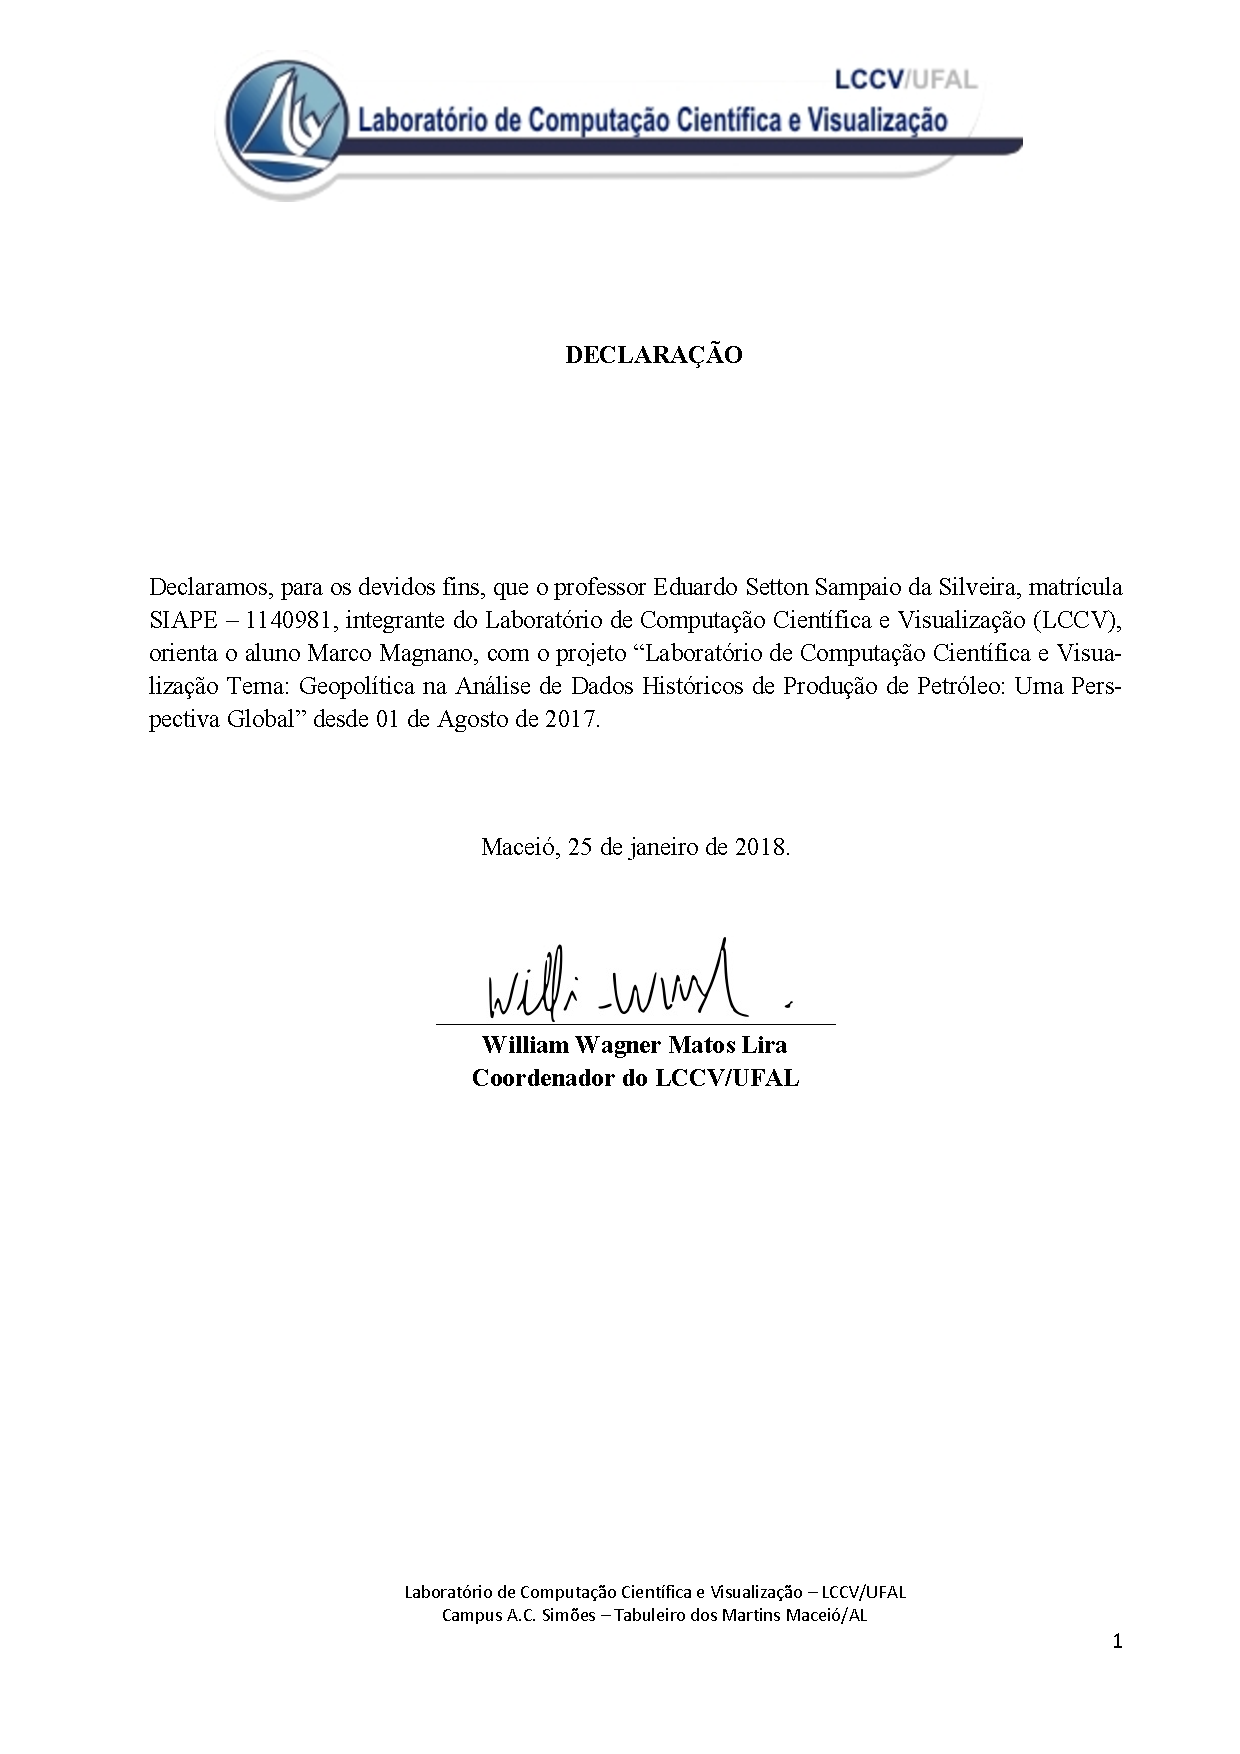
\includepdf[pages=-, scale=1,pagecommand=\thispagestyle{empty}]{\detokenize{GRUPO 1/Sub-Grupo 12/2017-ict-lccv1}}

\subsection{Orientação de estudantes de graduação em programas institucionalizados de pesquisa em andamento, por semestre}
\label{advisor:ict-lccv2}
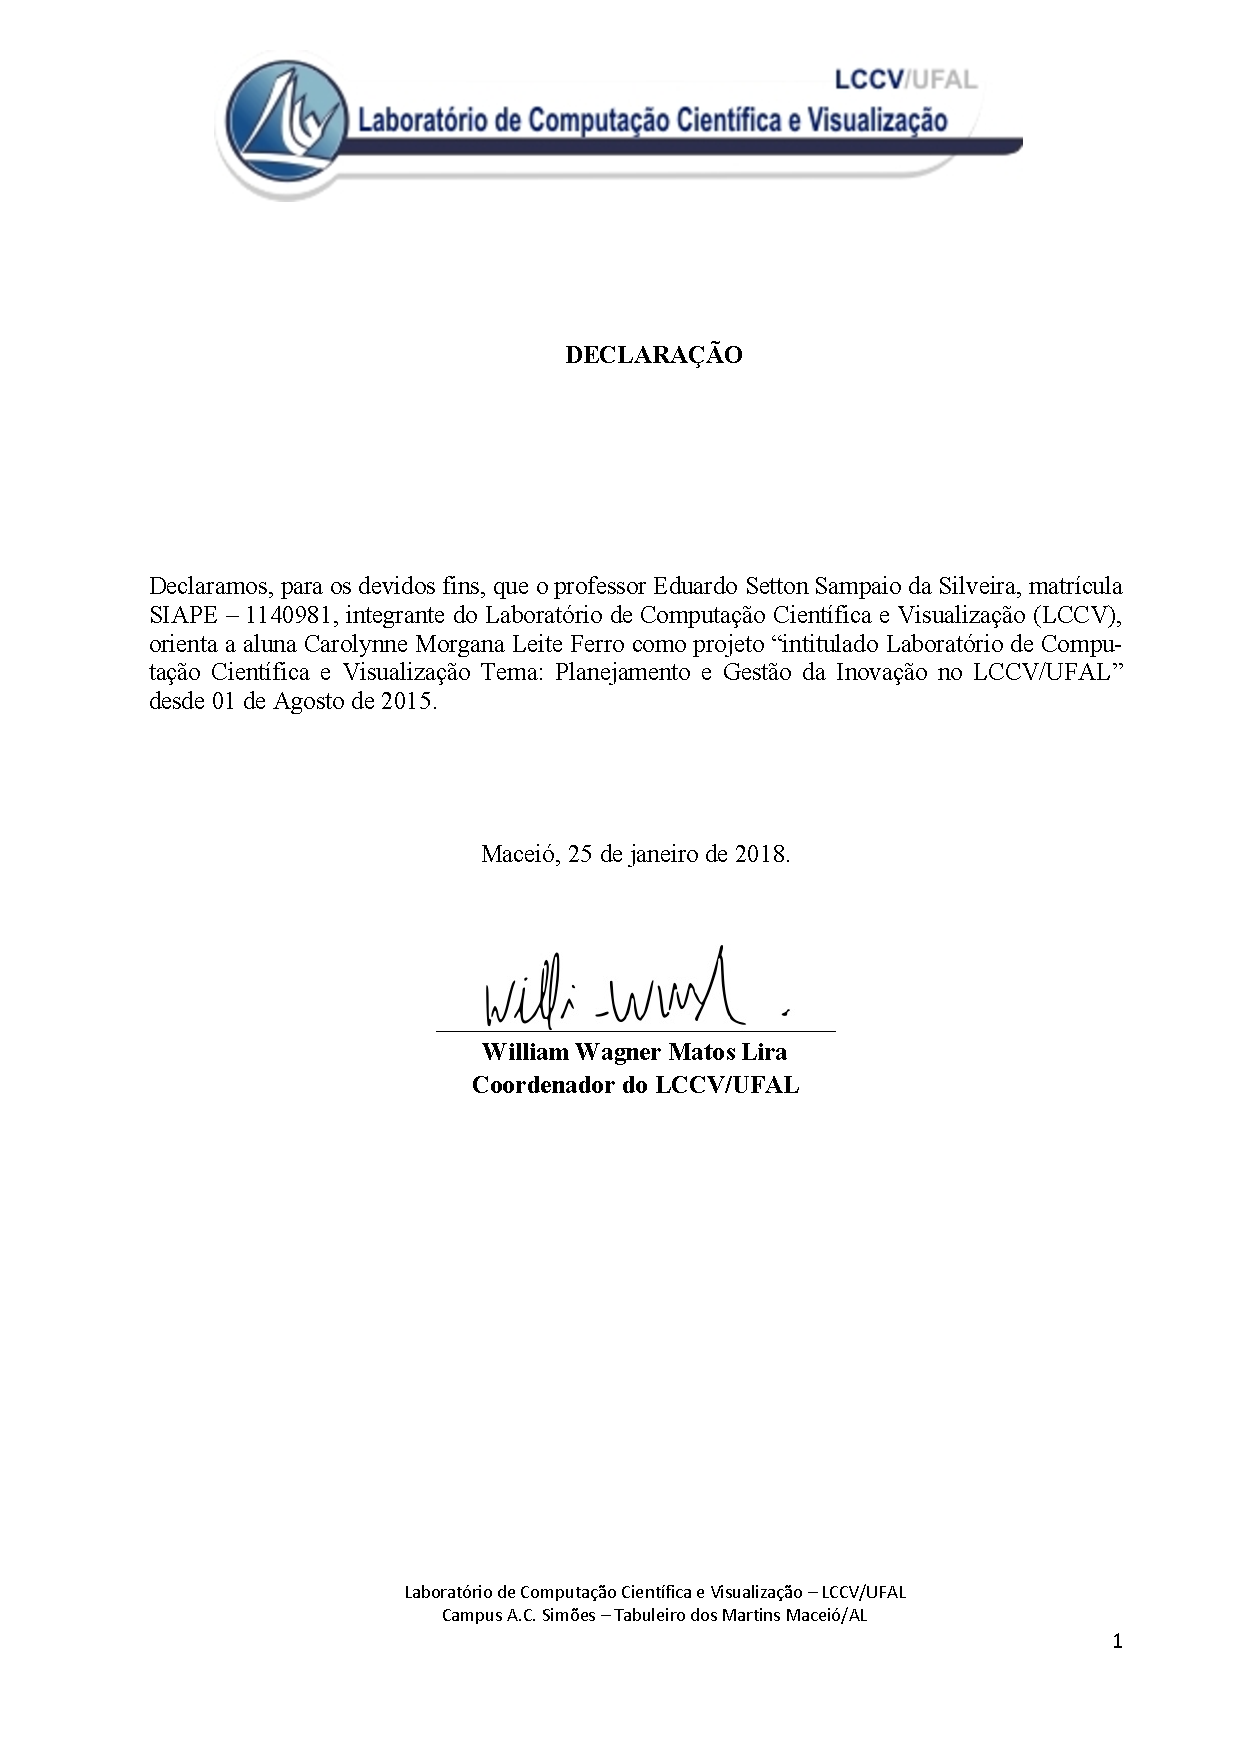
\includepdf[pages=-, scale=1,pagecommand=\thispagestyle{empty}]{\detokenize{GRUPO 1/Sub-Grupo 12/2017-ict-lccv2}}

\subsection{Orientação de estudantes de graduação em programas institucionalizados de pesquisa em andamento, por semestre}
\label{advisor:ict-pibit}
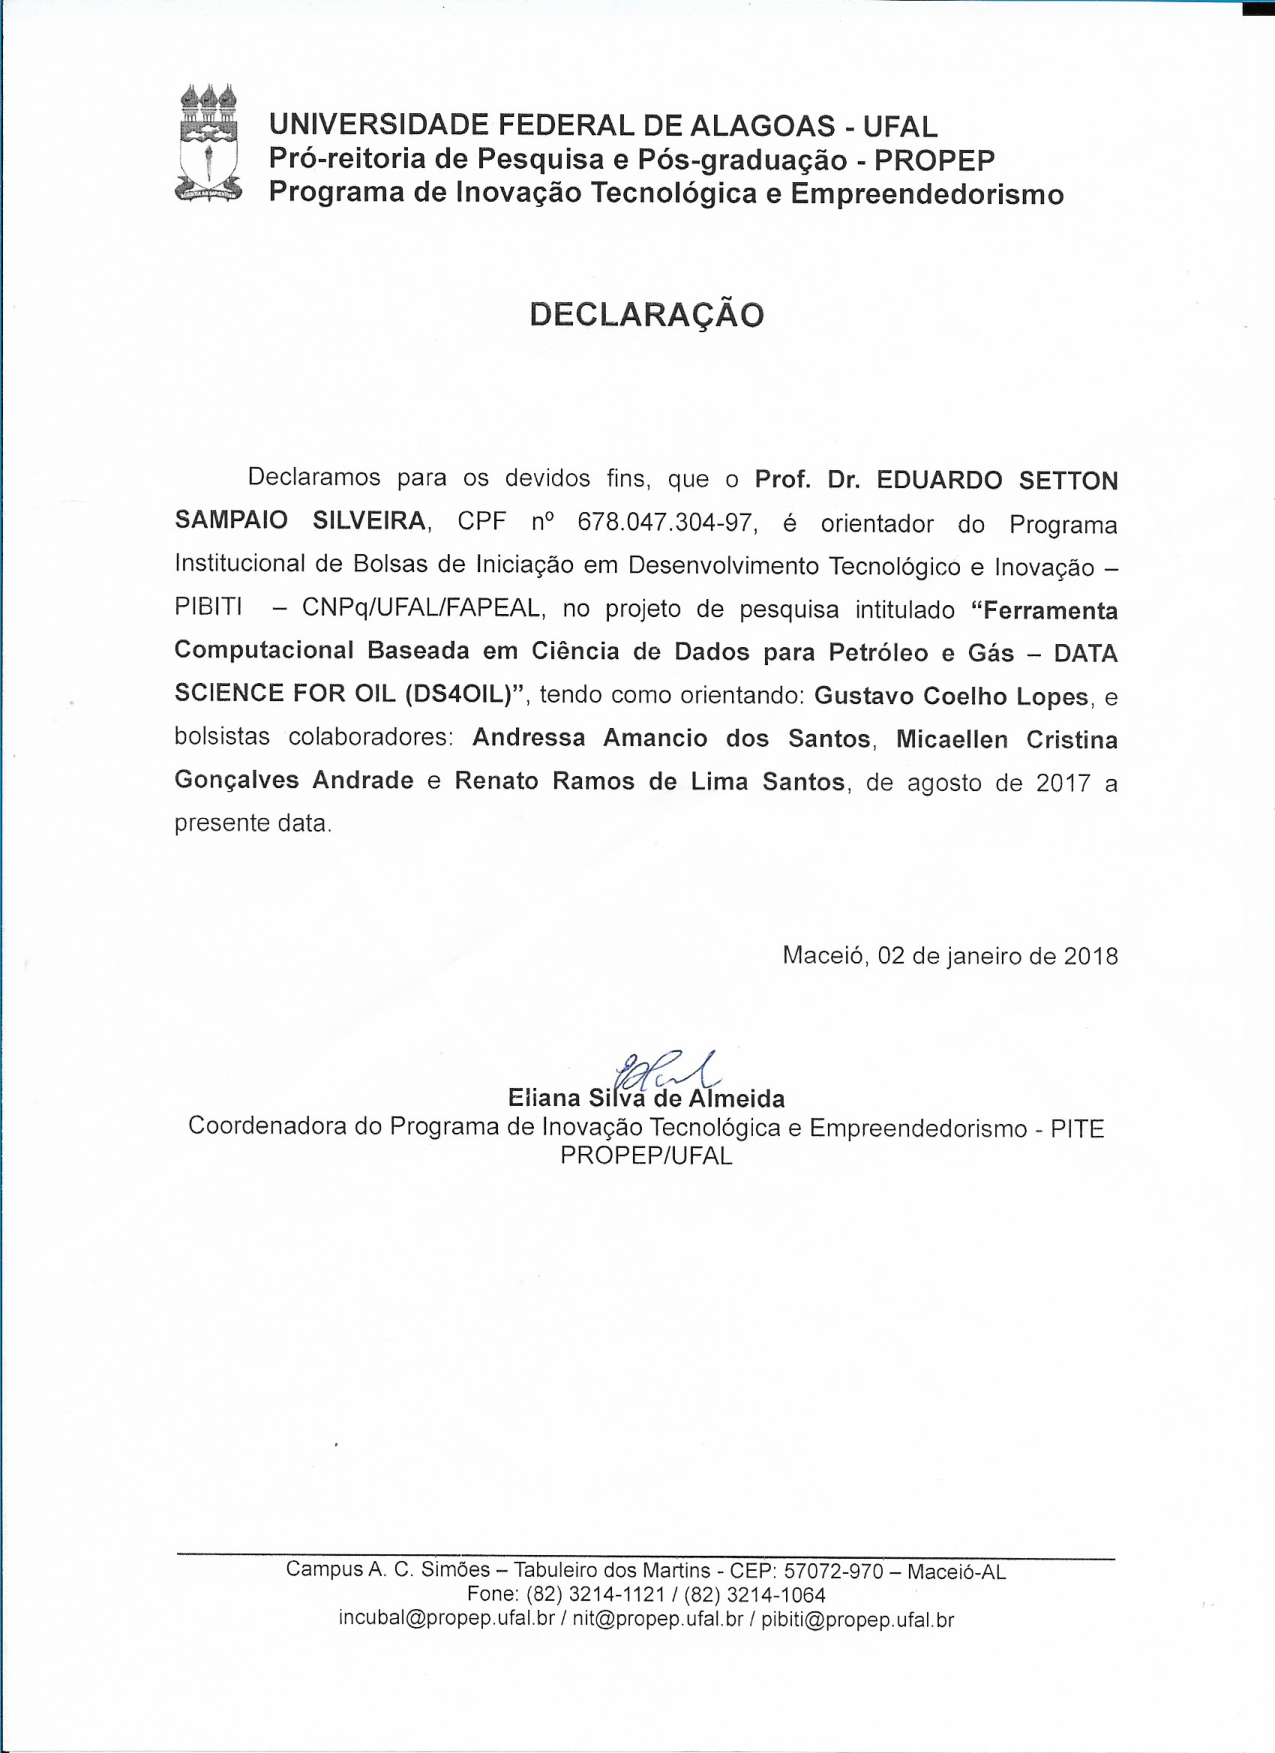
\includepdf[pages=-, scale=1,pagecommand=\thispagestyle{empty}]{\detokenize{GRUPO 1/Sub-Grupo 12/doc14}}

%%%%%%%%%%%%%%%%%%%%%%%%%%%%%%%%%%%%%%%%%%%%%%%%%%%%%%%%%%%%%%%%%%%%%%%%%%%%%%%
% Subgrupo 1.3 - Bancas
%%%%%%%%%%%%%%%%%%%%%%%%%%%%%%%%%%%%%%%%%%%%%%%%%%%%%%%%%%%%%%%%%%%%%%%%%%%%%%%

\newpage
\subsection{Participação em Banca de trabalhos de conclusão de cursos de graduação}
\label{banca:tcc1}
Esta subseção apresenta o comprovante de de participação em Bancas de Trabalhos de Conclusão de Curso.
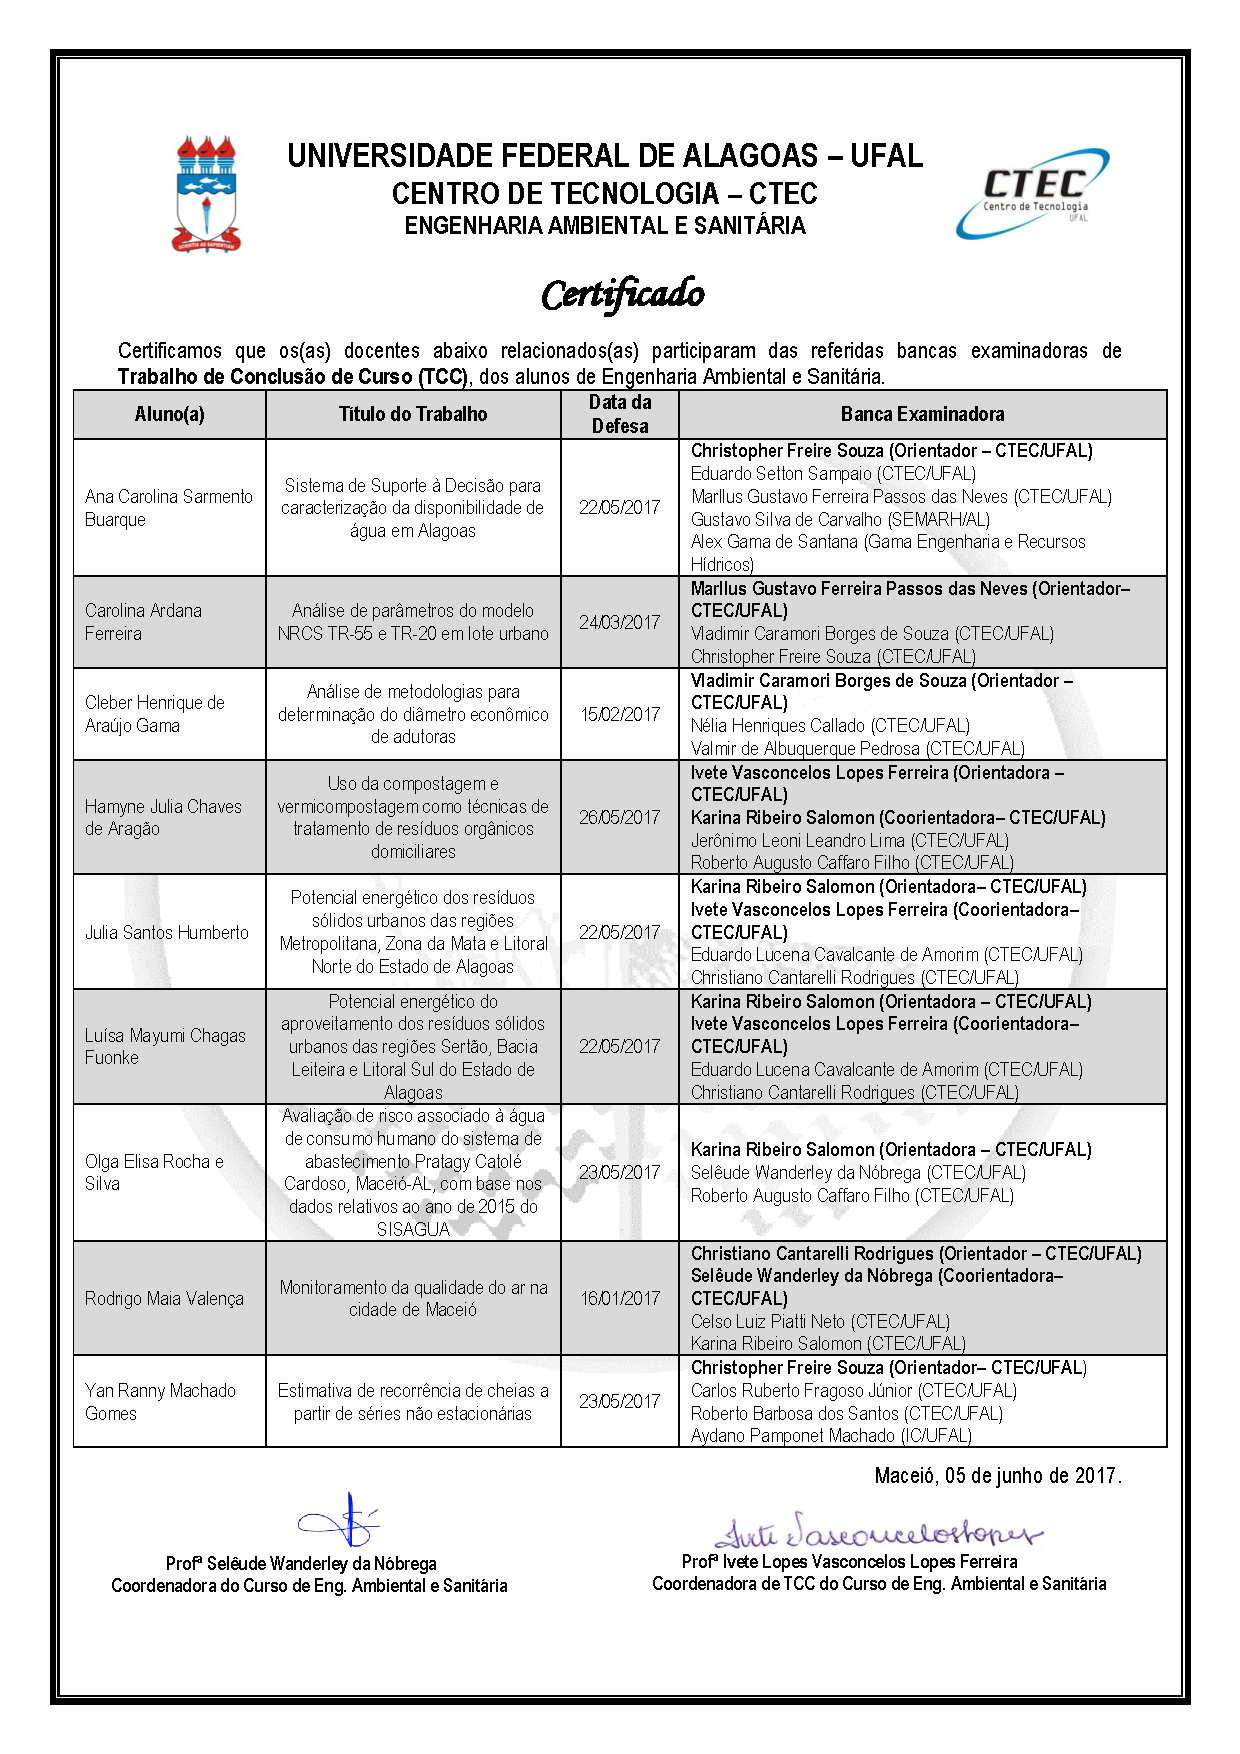
\includepdf[pages=-, scale=1,pagecommand=\thispagestyle{empty}]{\detokenize{GRUPO 1/Sub-Grupo 13/doc15}}
\subsection{Participação em Banca de trabalhos de conclusão de cursos de graduação}
\label{banca:tcc2}
Esta subseção apresenta o comprovante de de participação em Bancas de Trabalhos de Conclusão de Curso.
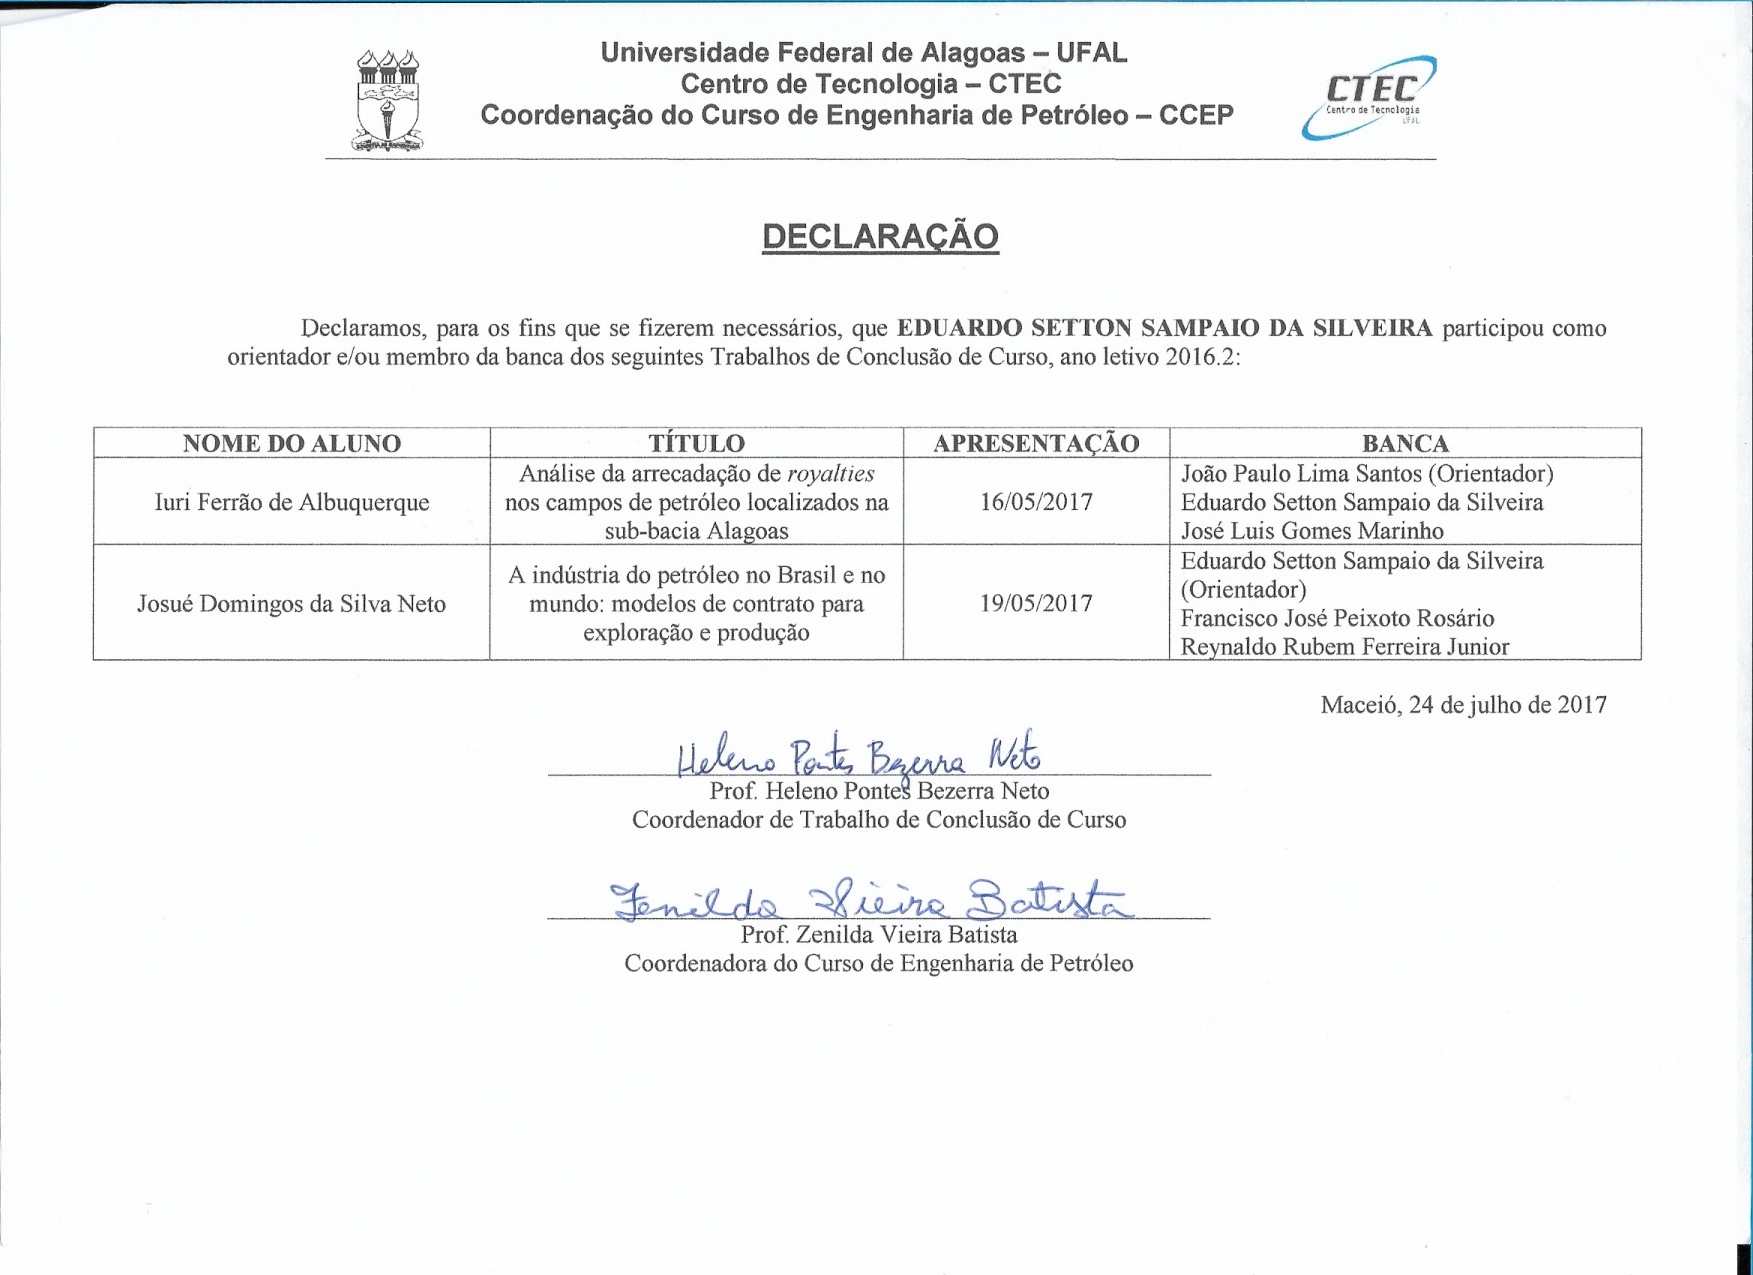
\includepdf[pages=-, scale=1,pagecommand=\thispagestyle{empty}]{\detokenize{GRUPO 1/Sub-Grupo 13/doc16}}
\subsection{Participação em Banca de trabalhos de conclusão de cursos de graduação}
\label{banca:tcc3}
Esta subseção apresenta o comprovante de de participação em Bancas de Trabalhos de Conclusão de Curso.
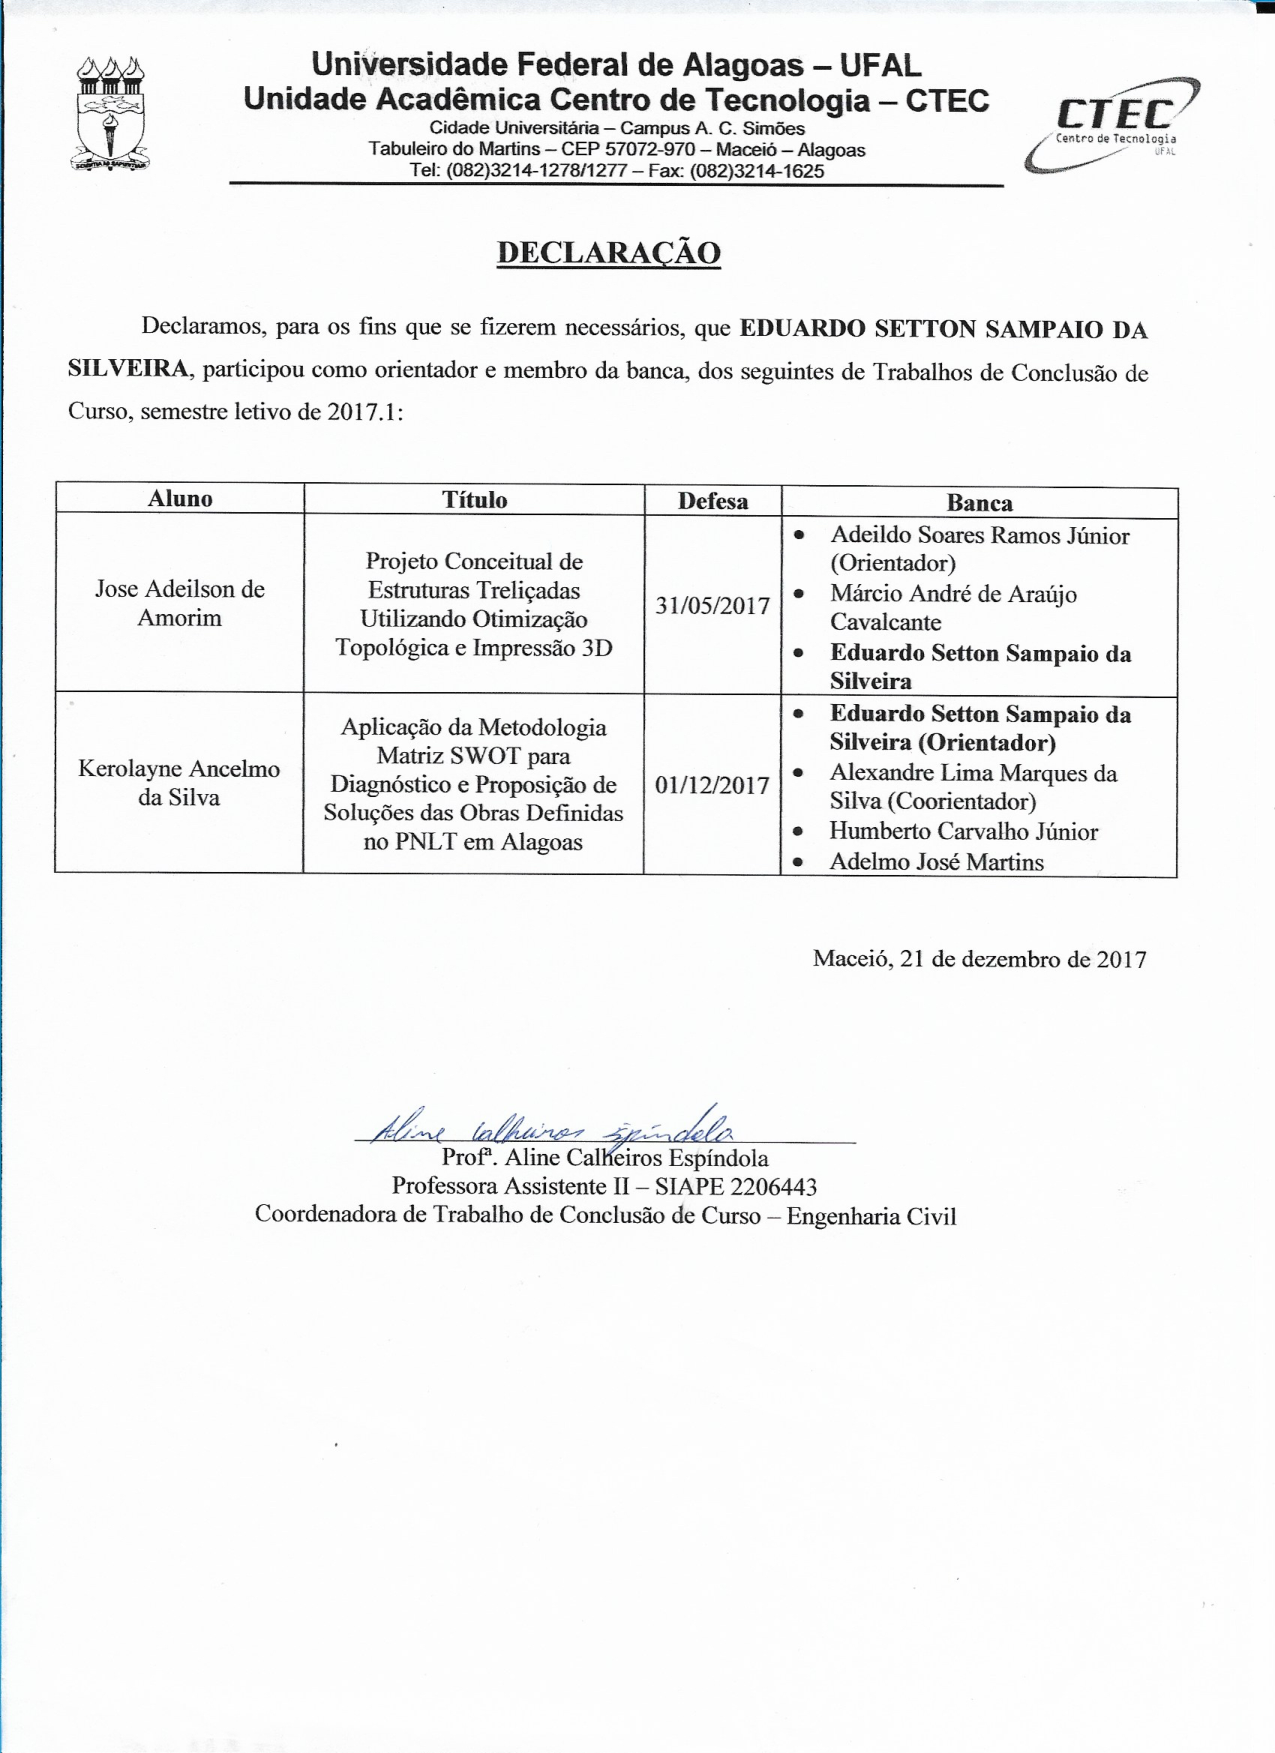
\includepdf[pages=-, scale=1,pagecommand=\thispagestyle{empty}]{\detokenize{GRUPO 1/Sub-Grupo 13/doc17}}

\newpage
\subsection{Participação em Banca de seleção de tutoria/monitoria}
\label{banca:2017-monitoria}
Esta subseção apresenta o comprovante de participação em banca de seleção de monitoria.
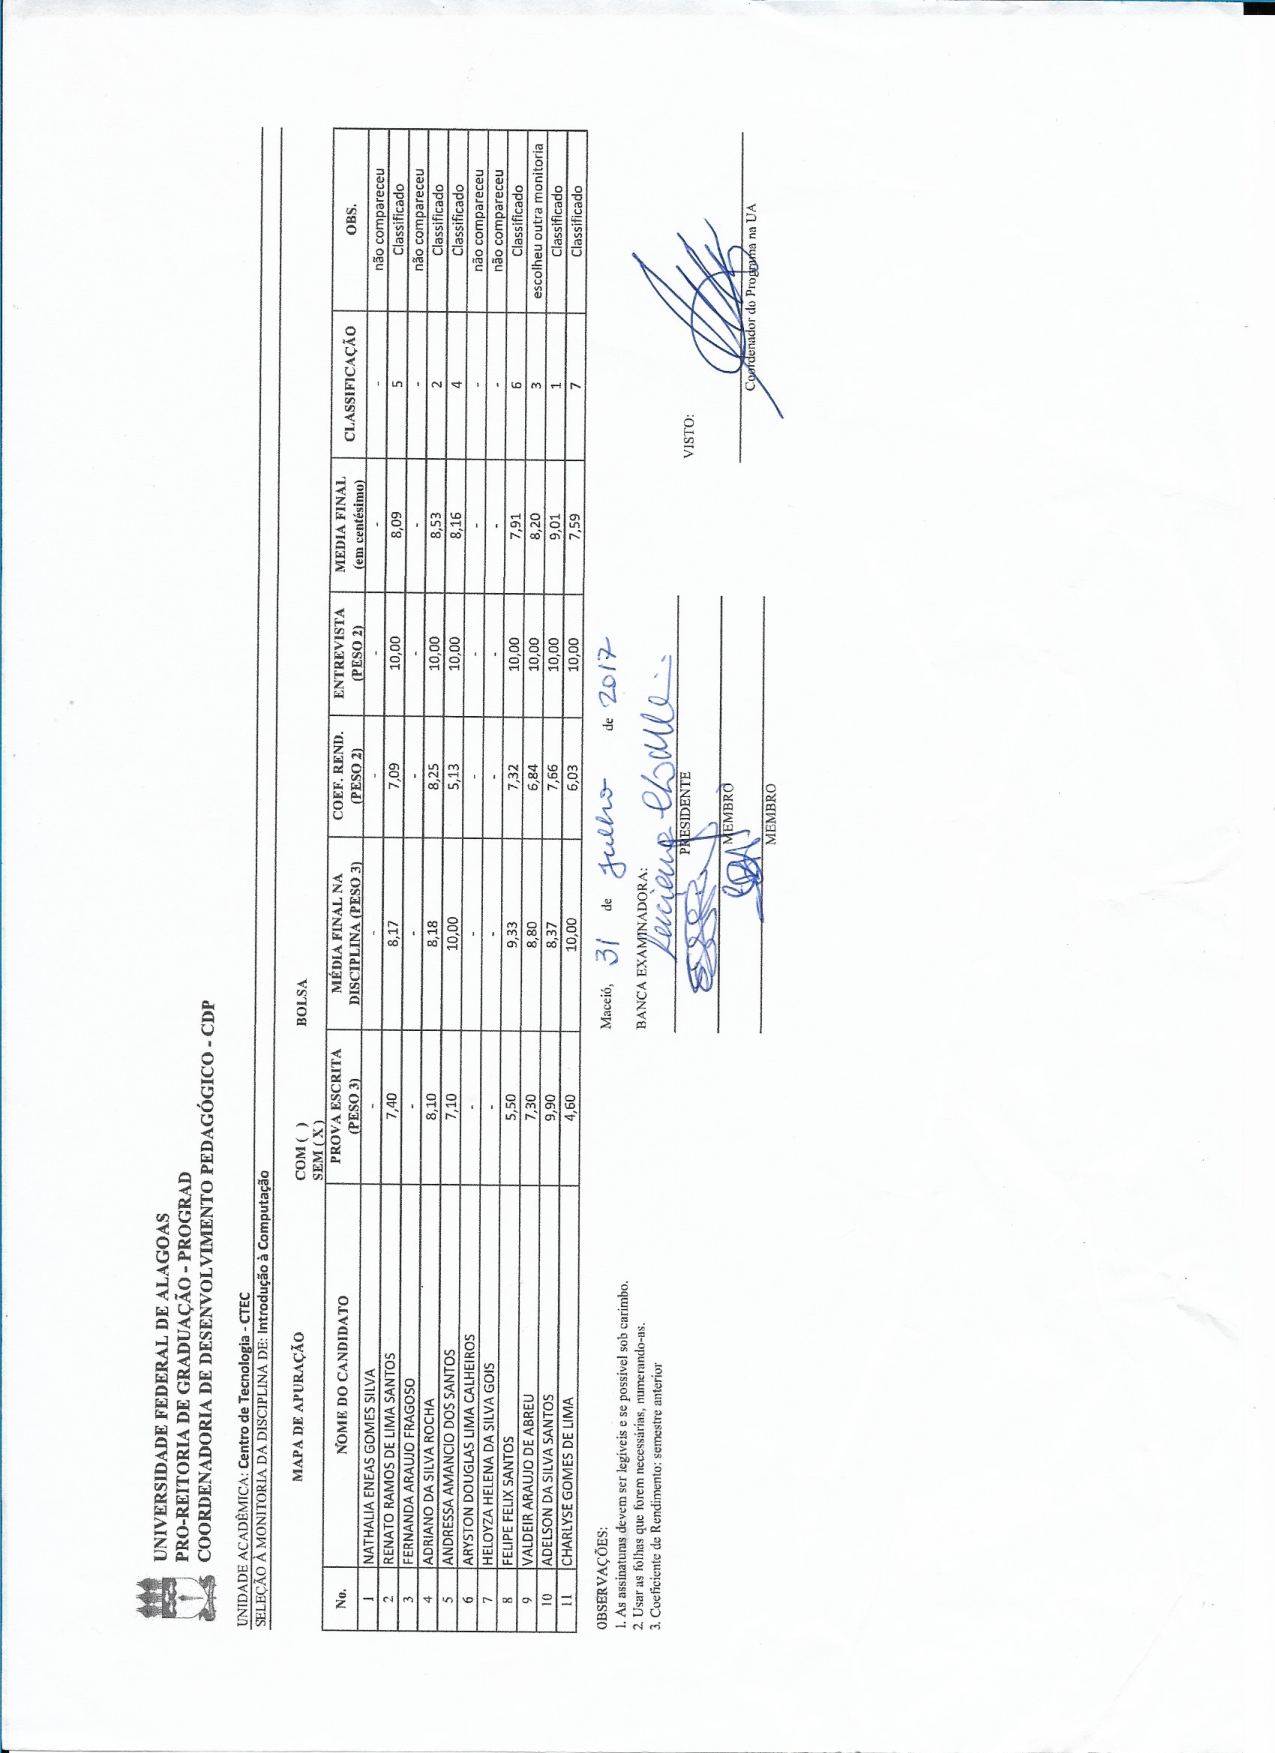
\includepdf[pages=-, scale=1, pagecommand=\thispagestyle{empty}]{\detokenize{GRUPO 1/Sub-Grupo 13/2017-monitoria}}

%%%%%%%%%%%%%%%%%%%%%%%%%%%%%%%%%%%%%%%%%%%%%%%%%%%%%%%%%%%%%%%%%%%%%%%%%%%%%%%
% Grupo 2 - Produção Intelectual
%%%%%%%%%%%%%%%%%%%%%%%%%%%%%%%%%%%%%%%%%%%%%%%%%%%%%%%%%%%%%%%%%%%%%%%%%%%%%%%

%%%%%%%%%%%%%%%%%%%%%%%%%%%%%%%%%%%%%%%%%%%%%%%%%%%%%%%%%%%%%%%%%%%%%%%%%%%%%%%
% Subgrupo 2.1 - Livro Publicado
%%%%%%%%%%%%%%%%%%%%%%%%%%%%%%%%%%%%%%%%%%%%%%%%%%%%%%%%%%%%%%%%%%%%%%%%%%%%%%%

\newpage
\subsection{Autor}
\label{prodtec:livro}
Esta subseção apresenta o comprovante de que participou como autor de livro publicado.
\includepdf[pages=-, scale=1, pagecommand=\thispagestyle{empty}]{\detokenize{GRUPO 2/Sub-Grupo 21/doc19}}

%%%%%%%%%%%%%%%%%%%%%%%%%%%%%%%%%%%%%%%%%%%%%%%%%%%%%%%%%%%%%%%%%%%%%%%%%%%%%%%
% Subgrupo 2.2 - Artigo Publicado
%%%%%%%%%%%%%%%%%%%%%%%%%%%%%%%%%%%%%%%%%%%%%%%%%%%%%%%%%%%%%%%%%%%%%%%%%%%%%%%
\newpage
\subsection{Artigo publicado em periódicos indexados (ISSN), registrados no Estrato Qualis/CAPES Categoria B3 a B5 na respectiva área}
\label{journal:cadernos}
Esta subseção apresenta o comprovante de que participou como autor de livro publicado.
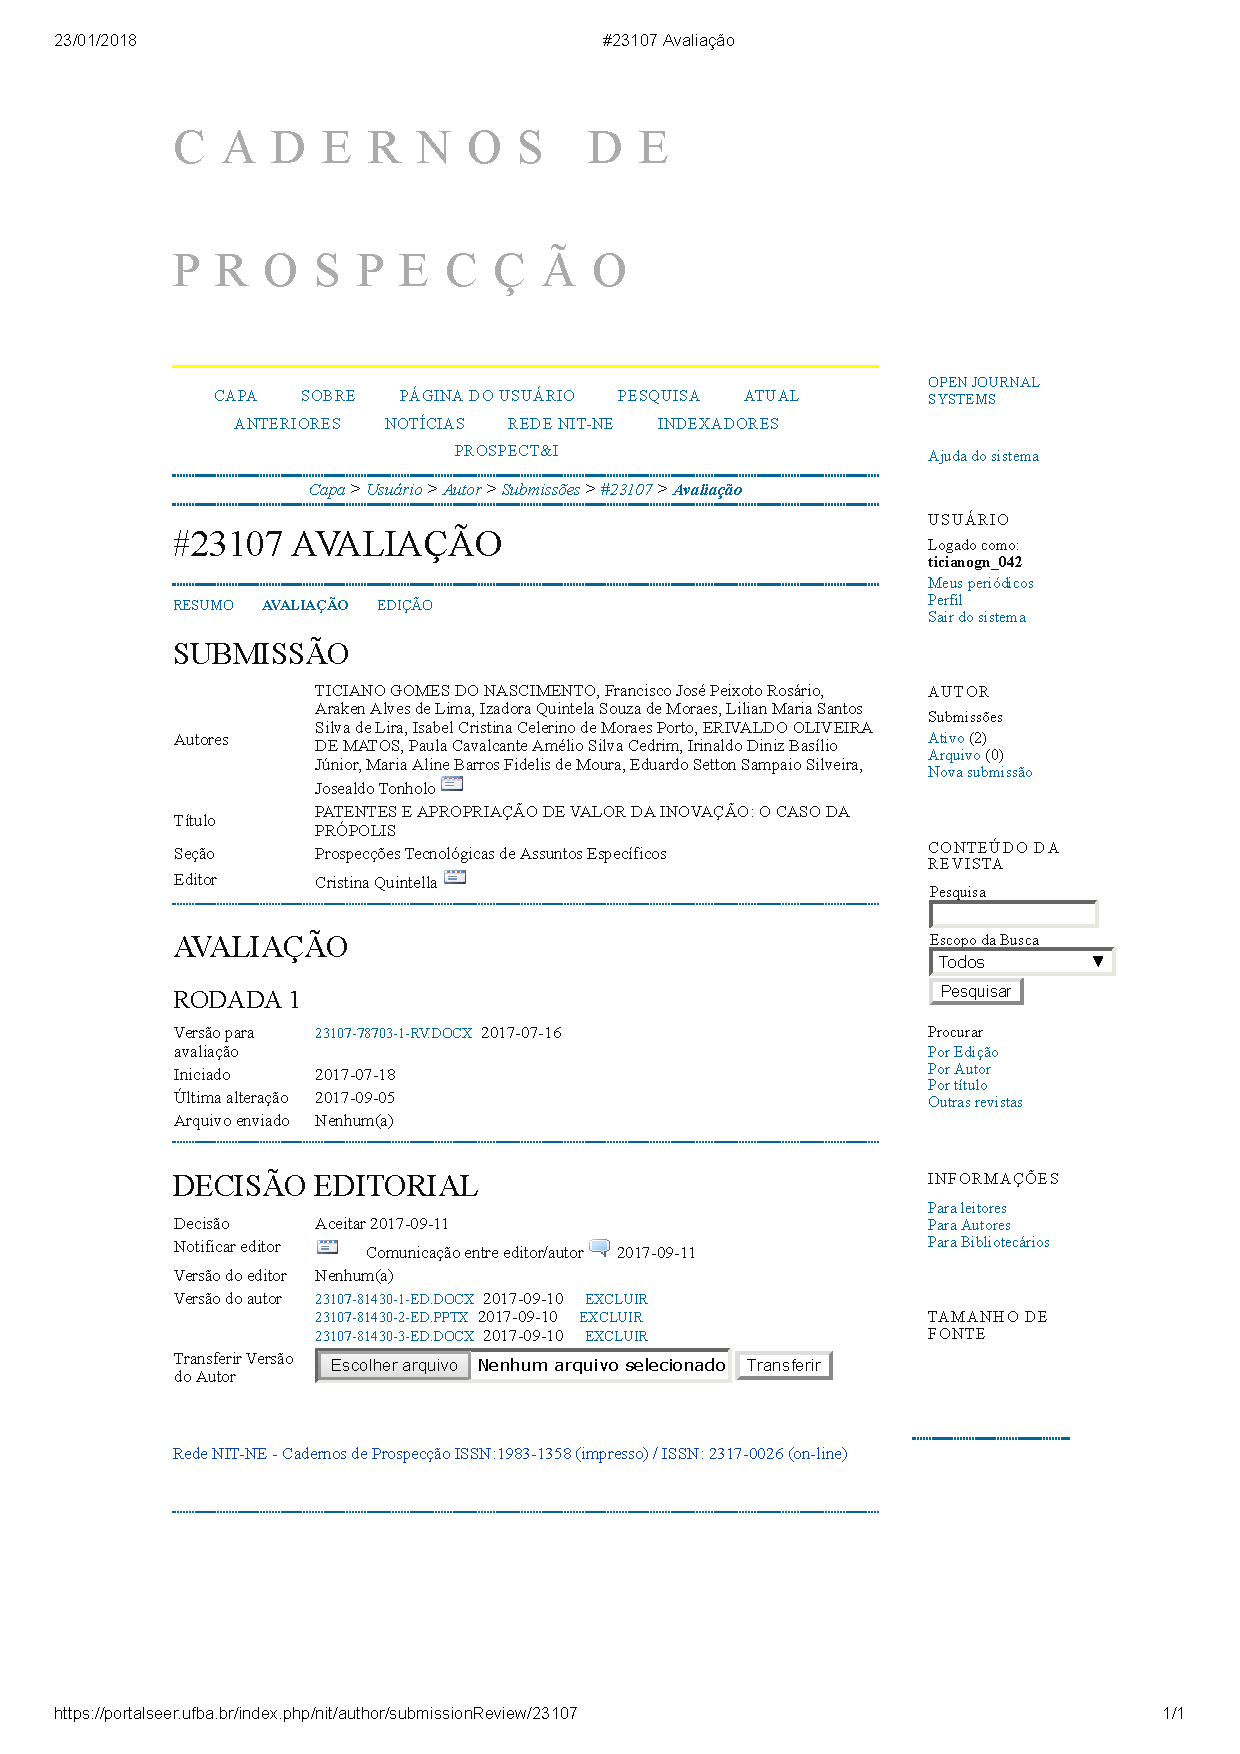
\includepdf[pages=-, scale=1, pagecommand=\thispagestyle{empty}]{\detokenize{GRUPO 2/Sub-Grupo 22/cadernos1}}
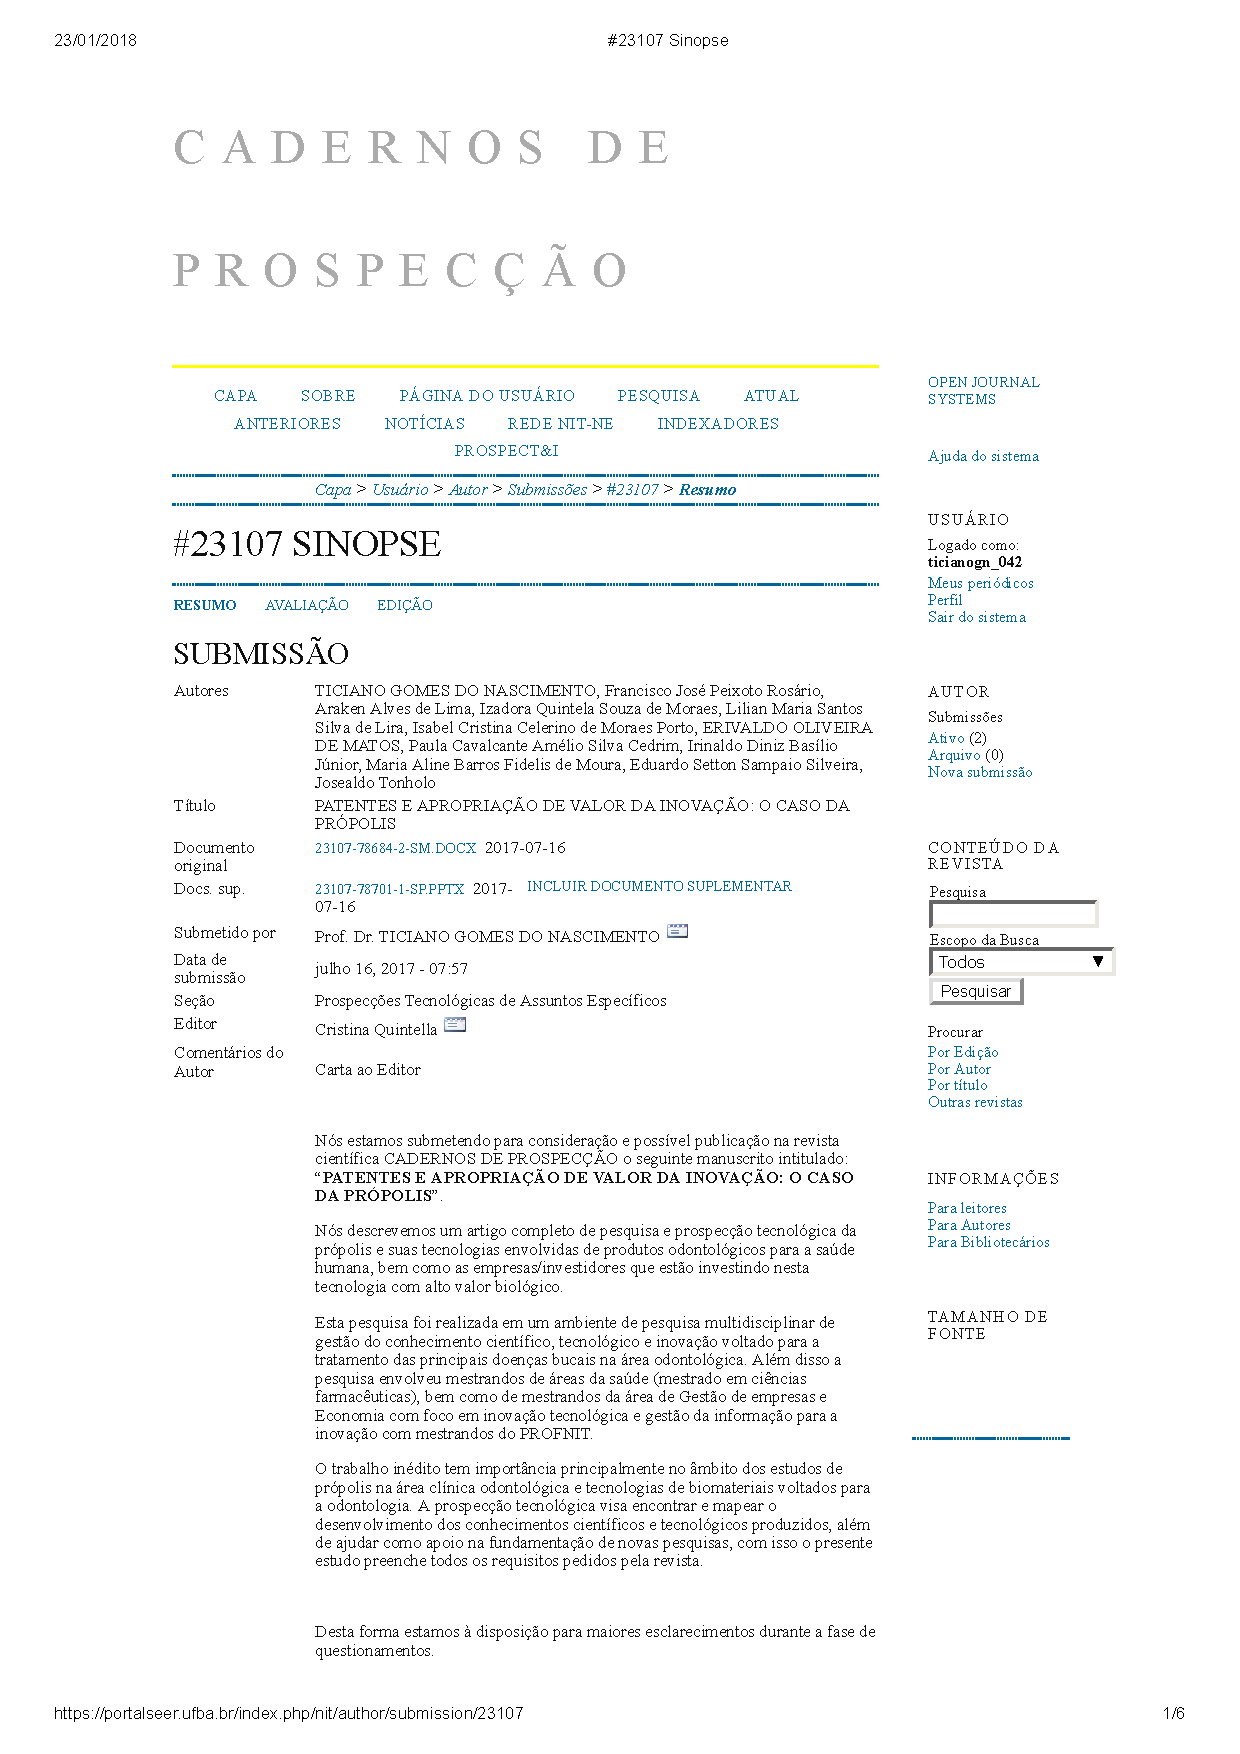
\includepdf[pages=-, scale=1, pagecommand=\thispagestyle{empty}]{\detokenize{GRUPO 2/Sub-Grupo 22/cadernos2}}
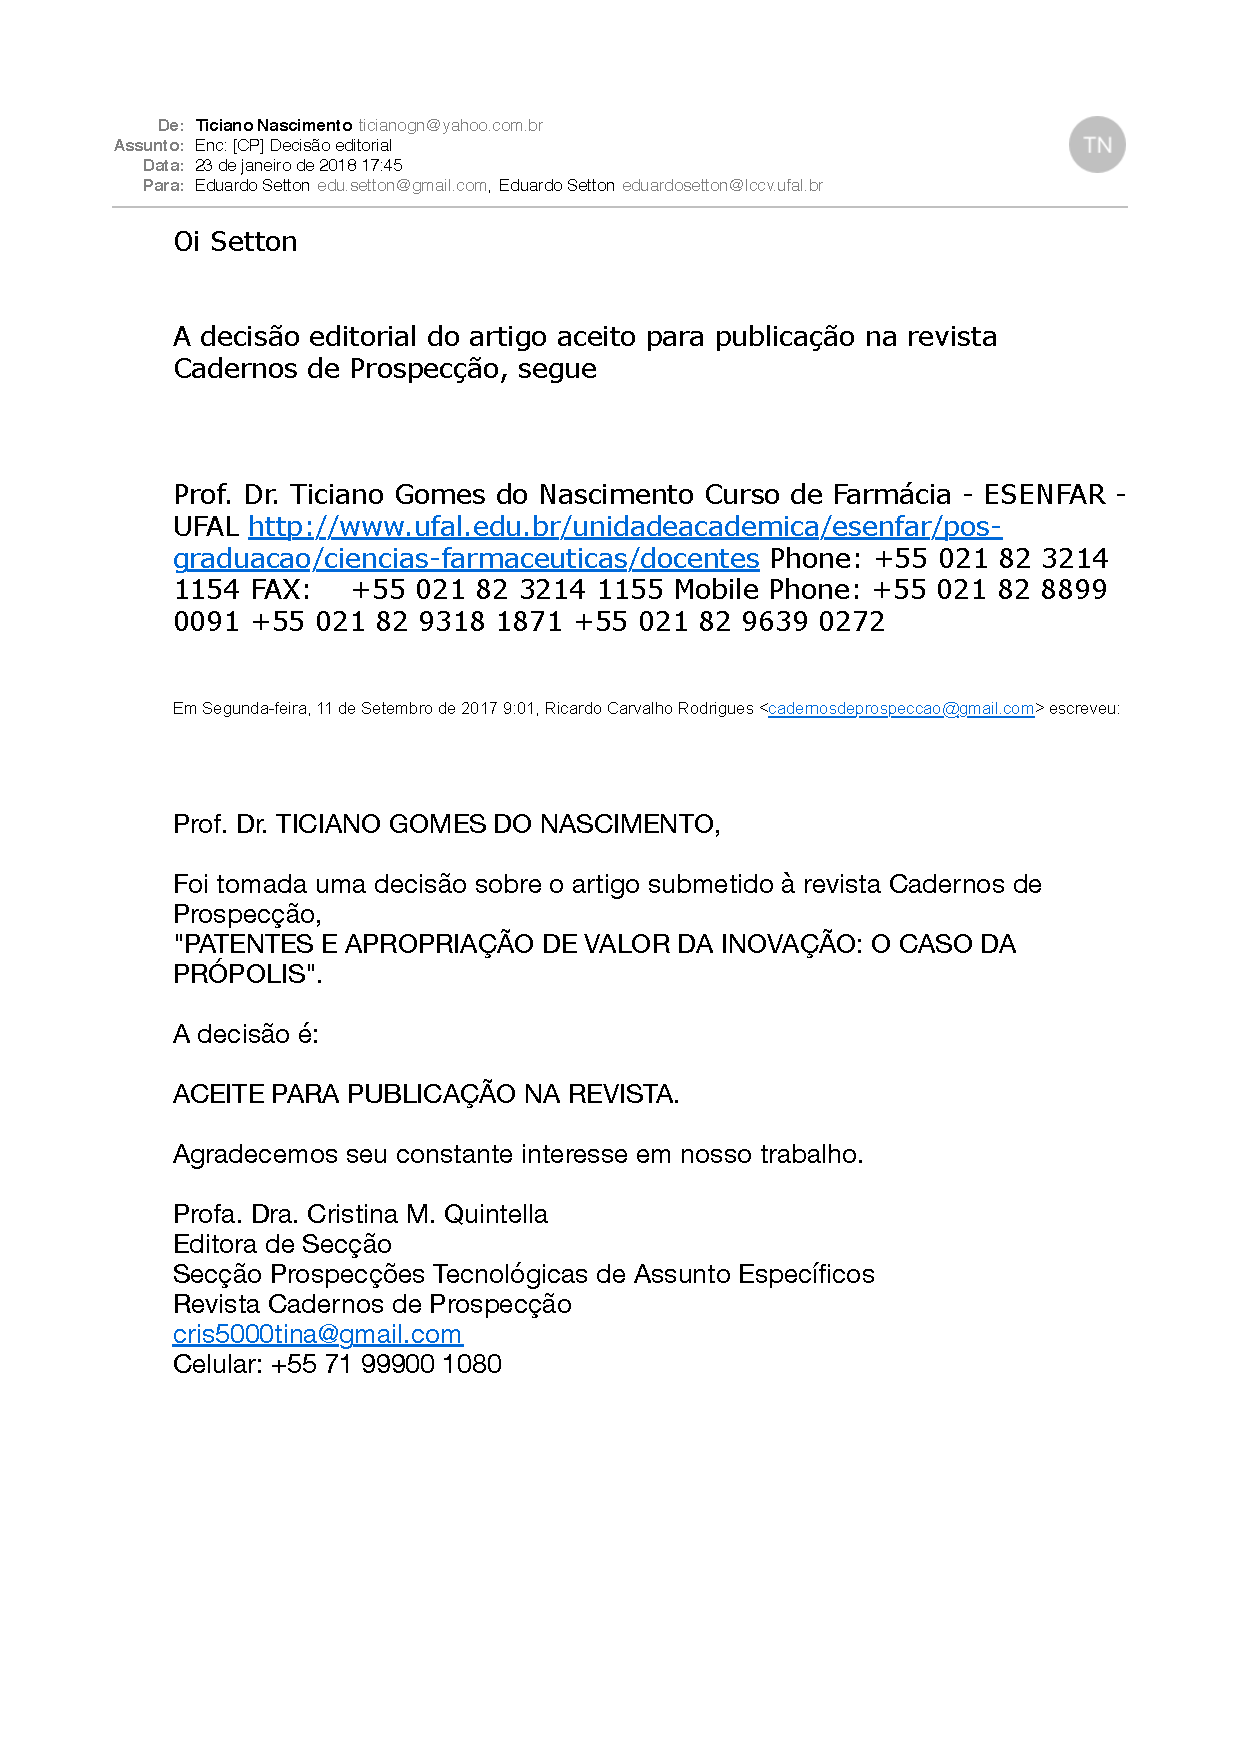
\includepdf[pages=-, scale=1, pagecommand=\thispagestyle{empty}]{\detokenize{GRUPO 2/Sub-Grupo 22/cadernos3}}

%%%%%%%%%%%%%%%%%%%%%%%%%%%%%%%%%%%%%%%%%%%%%%%%%%%%%%%%%%%%%%%%%%%%%%%%%%%%%%%
% Subgrupo 2.3 - Parecer Técnico
%%%%%%%%%%%%%%%%%%%%%%%%%%%%%%%%%%%%%%%%%%%%%%%%%%%%%%%%%%%%%%%%%%%%%%%%%%%%%%%

\newpage
\subsection{Parecer técnico na área de atuação do Docente}
\label{parecer:fapesp1}
Esta subseção apresenta o comprovante de atuação em Parecer técnico na área de atuação do Docente.
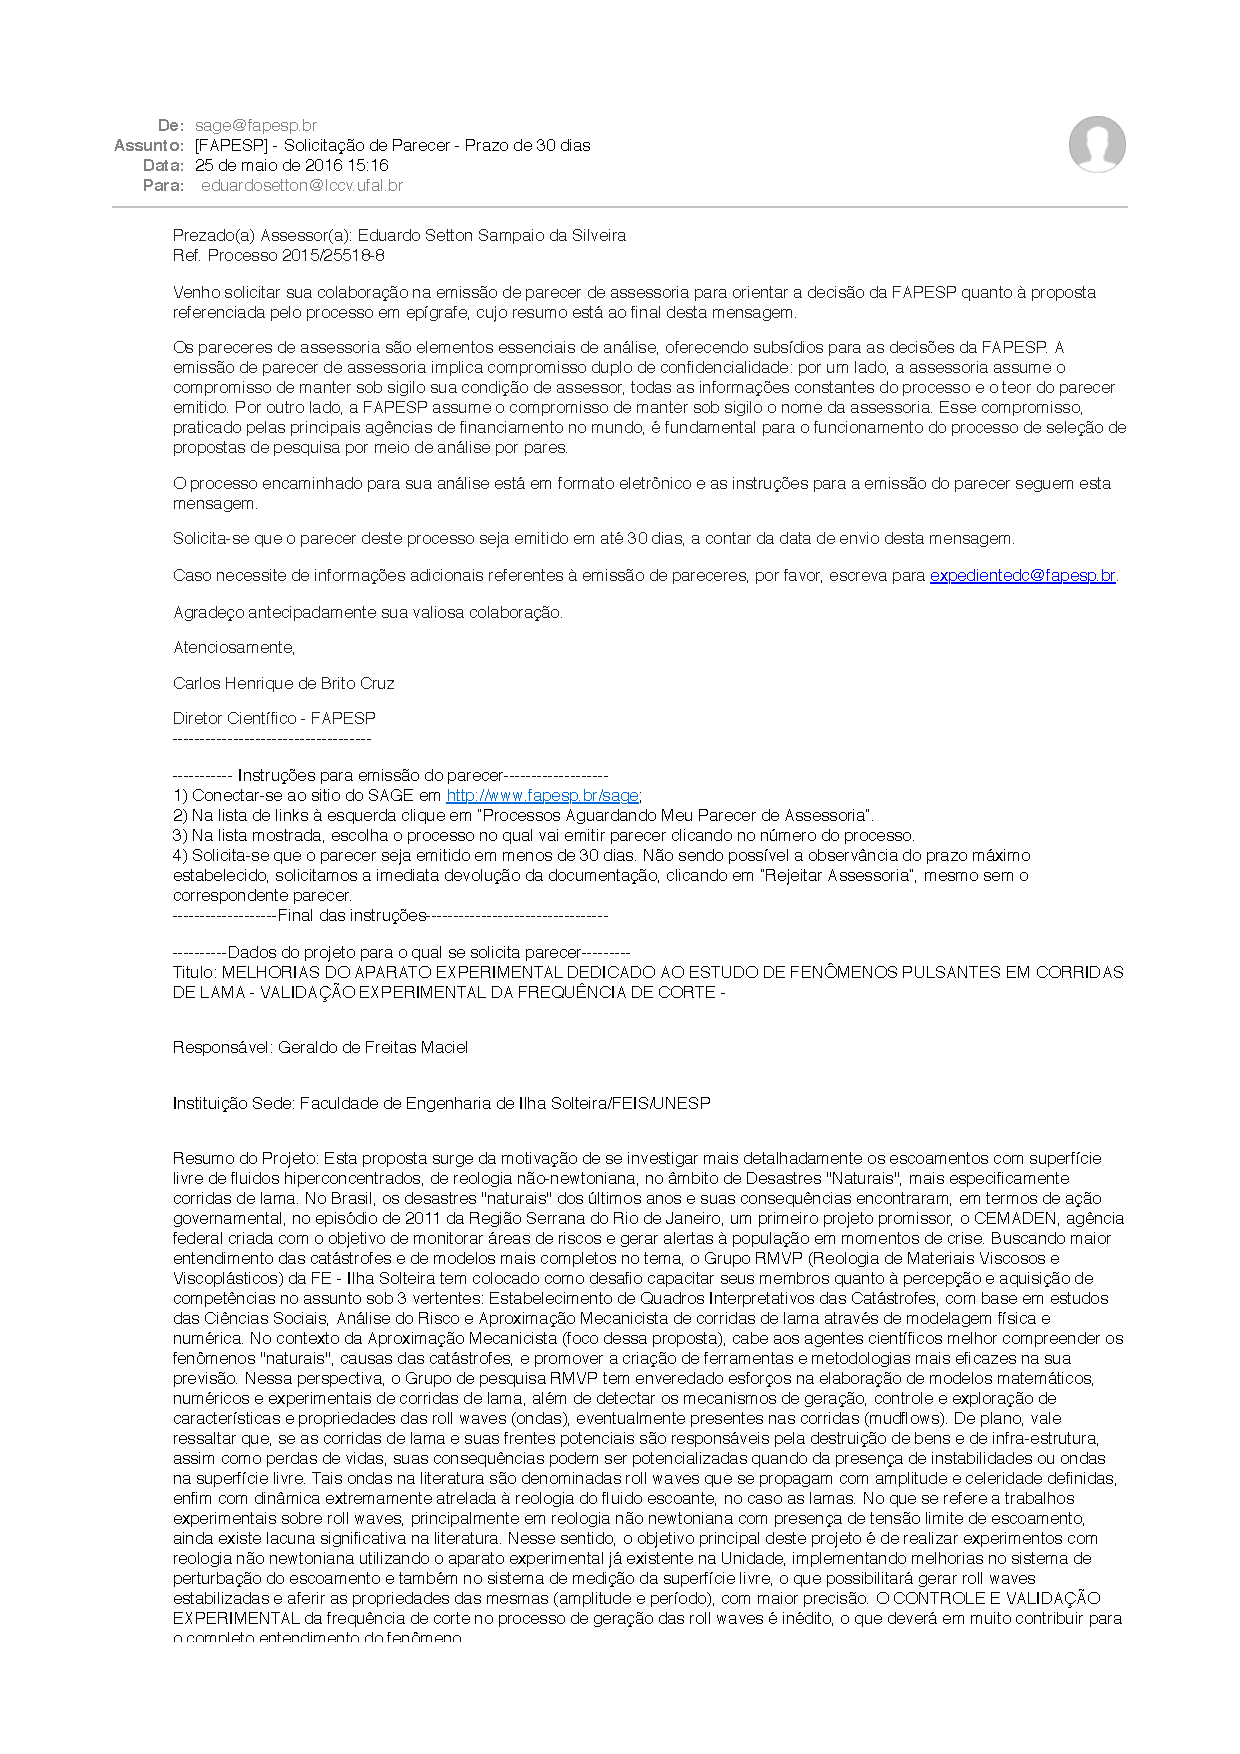
\includepdf[pages=-, scale=1, pagecommand=\thispagestyle{empty}]{\detokenize{GRUPO 2/Sub-Grupo 23/solfapesp1}}
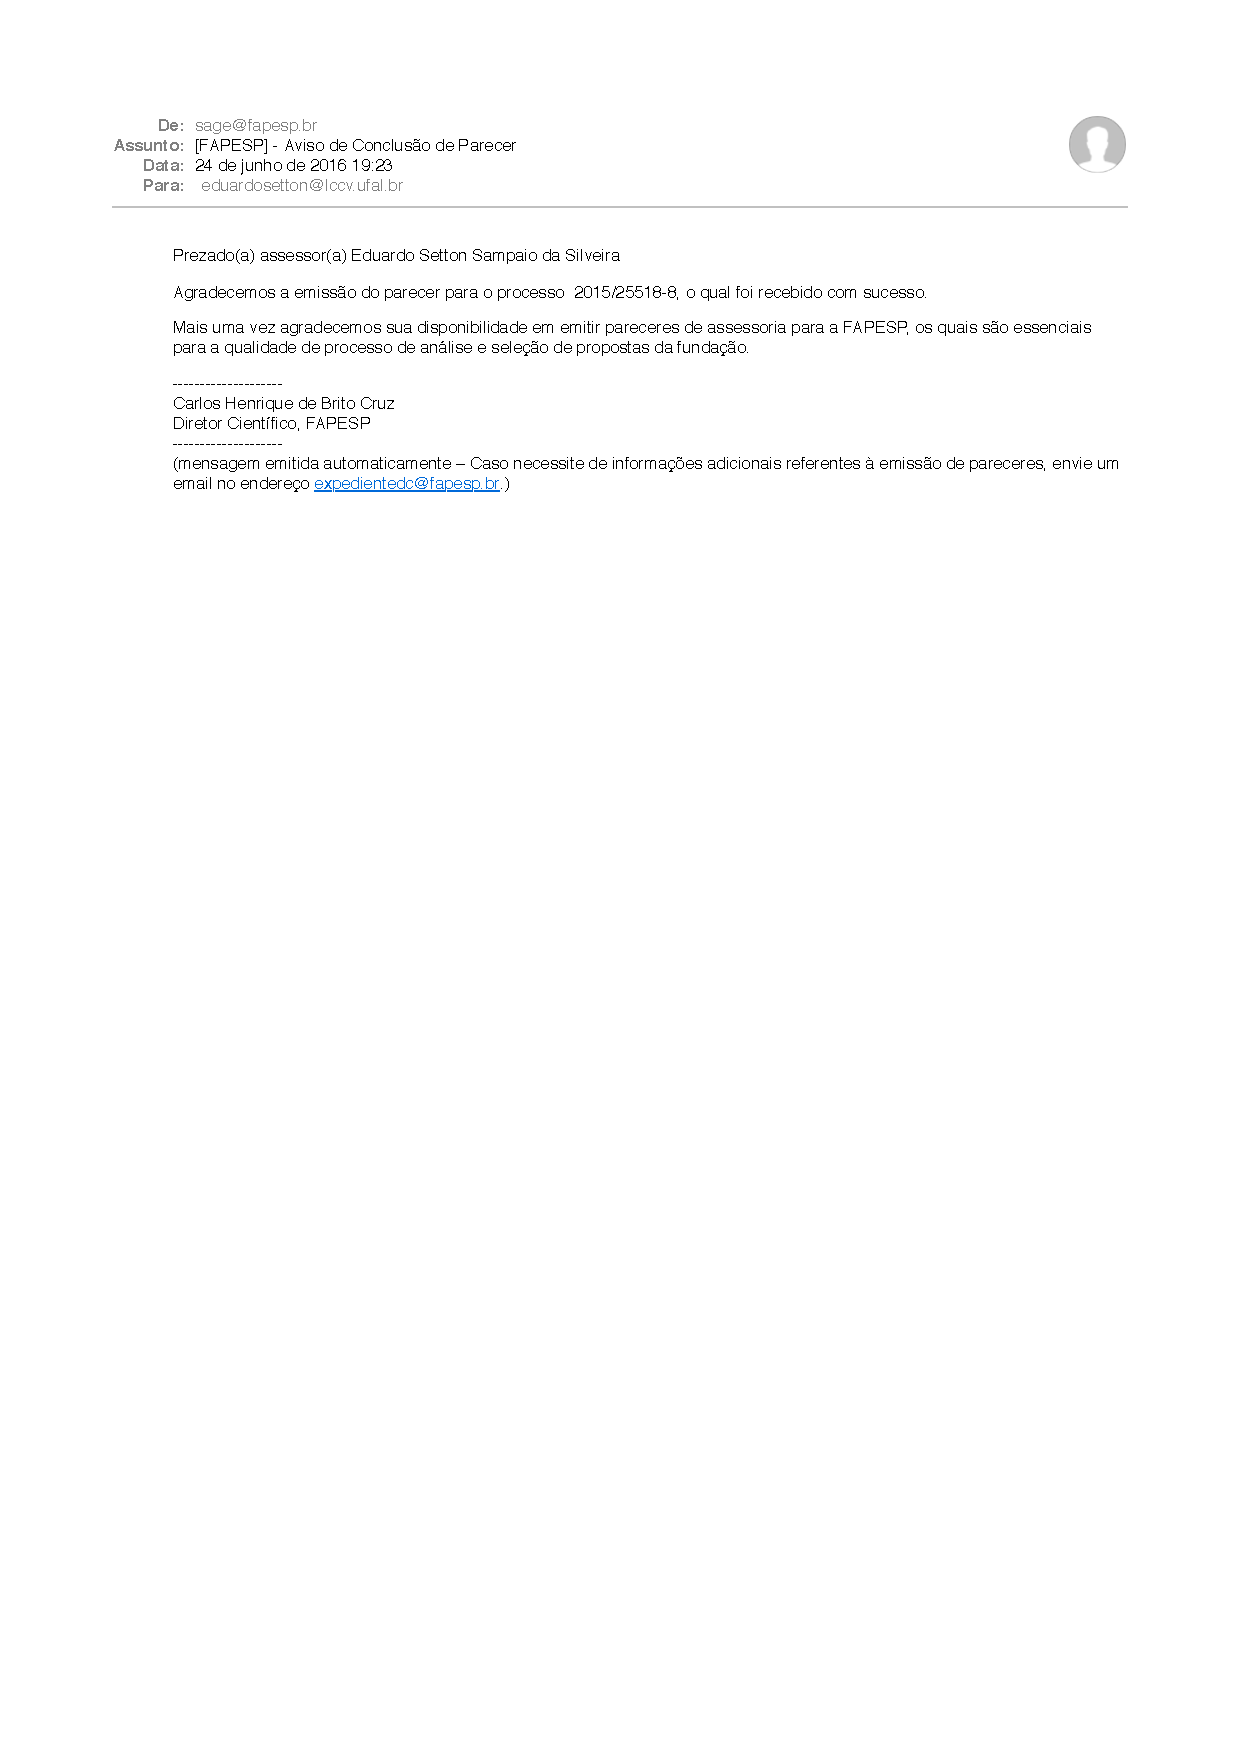
\includepdf[pages=-, scale=1, pagecommand=\thispagestyle{empty}]{\detokenize{GRUPO 2/Sub-Grupo 23/concfapesp1}}

\subsection{Parecer técnico na área de atuação do Docente}
\label{parecer:fapesp2}
Esta subseção apresenta o comprovante de atuação em Parecer técnico na área de atuação do Docente.
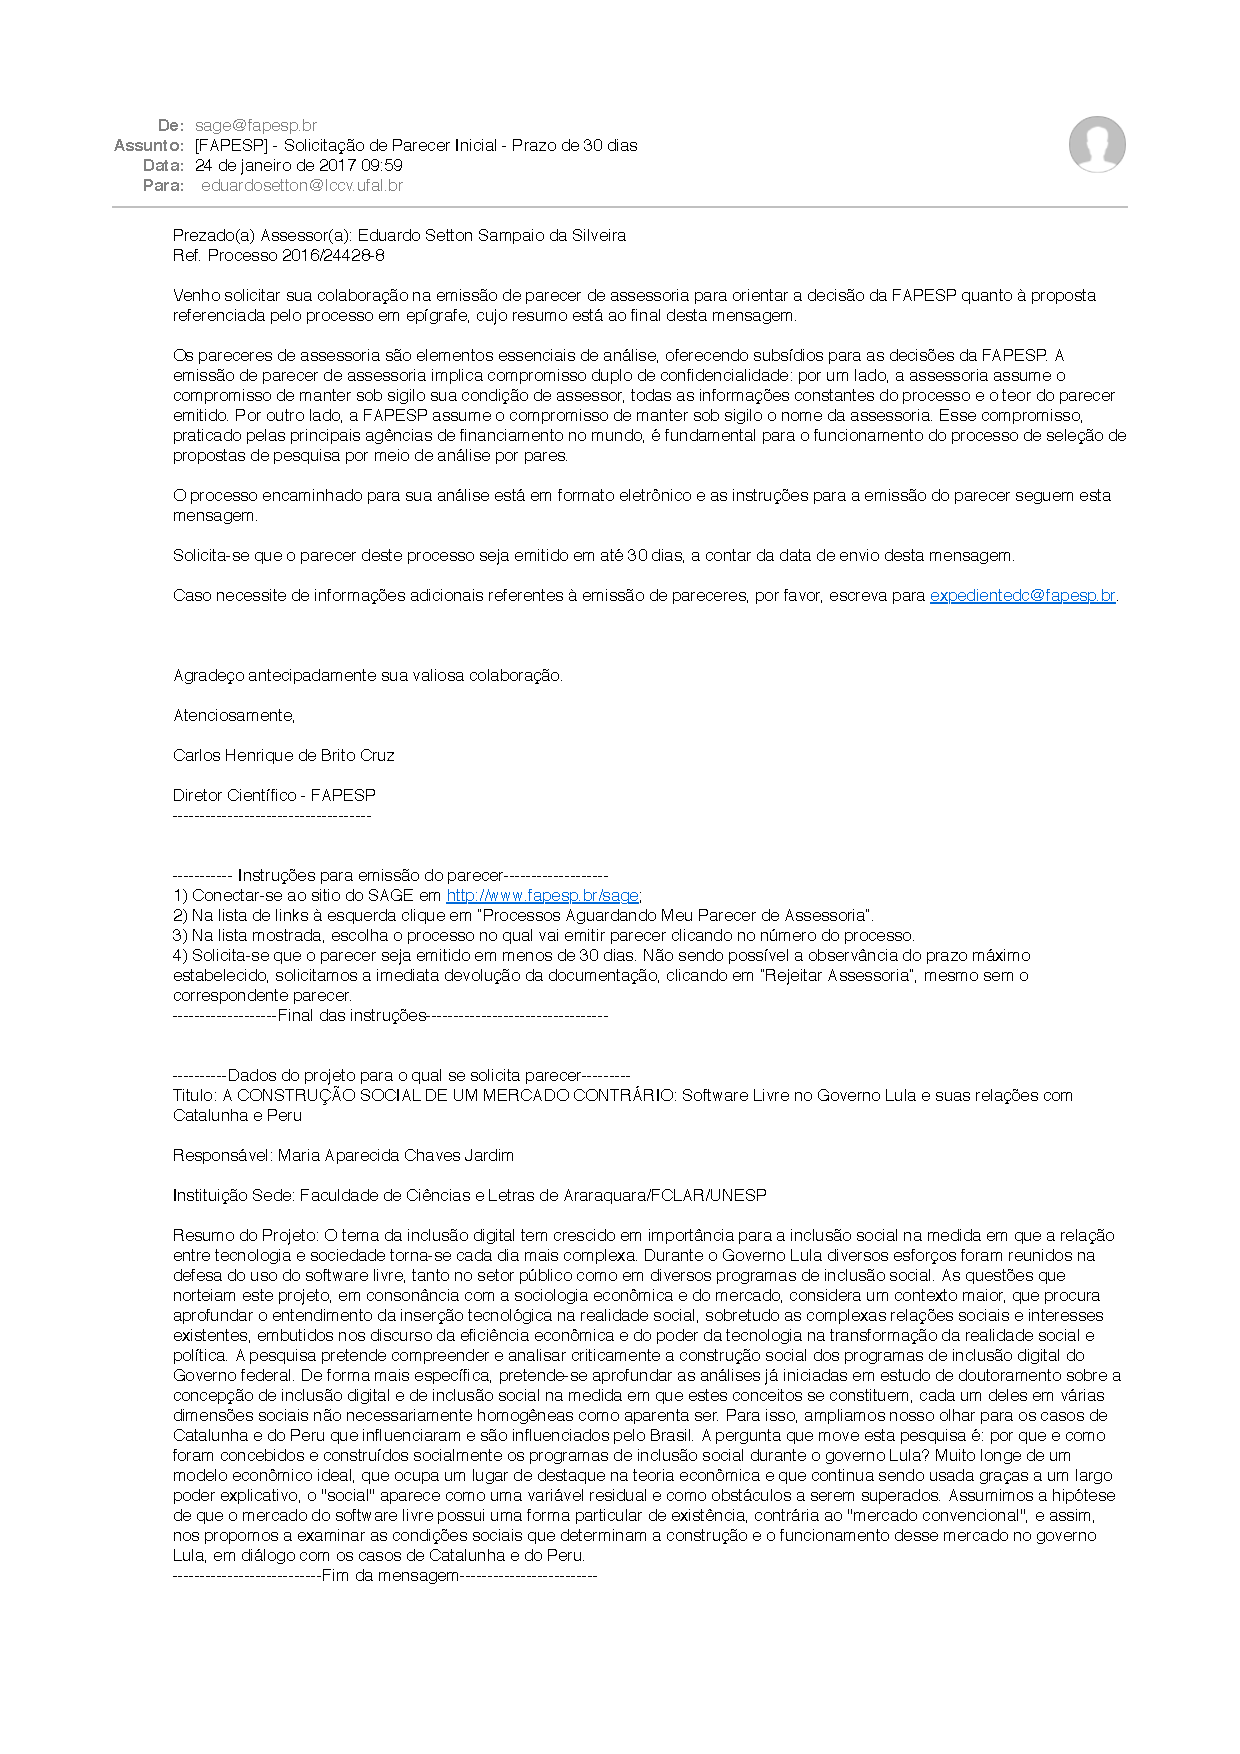
\includepdf[pages=-, scale=1, pagecommand=\thispagestyle{empty}]{\detokenize{GRUPO 2/Sub-Grupo 23/solfapesp2}}
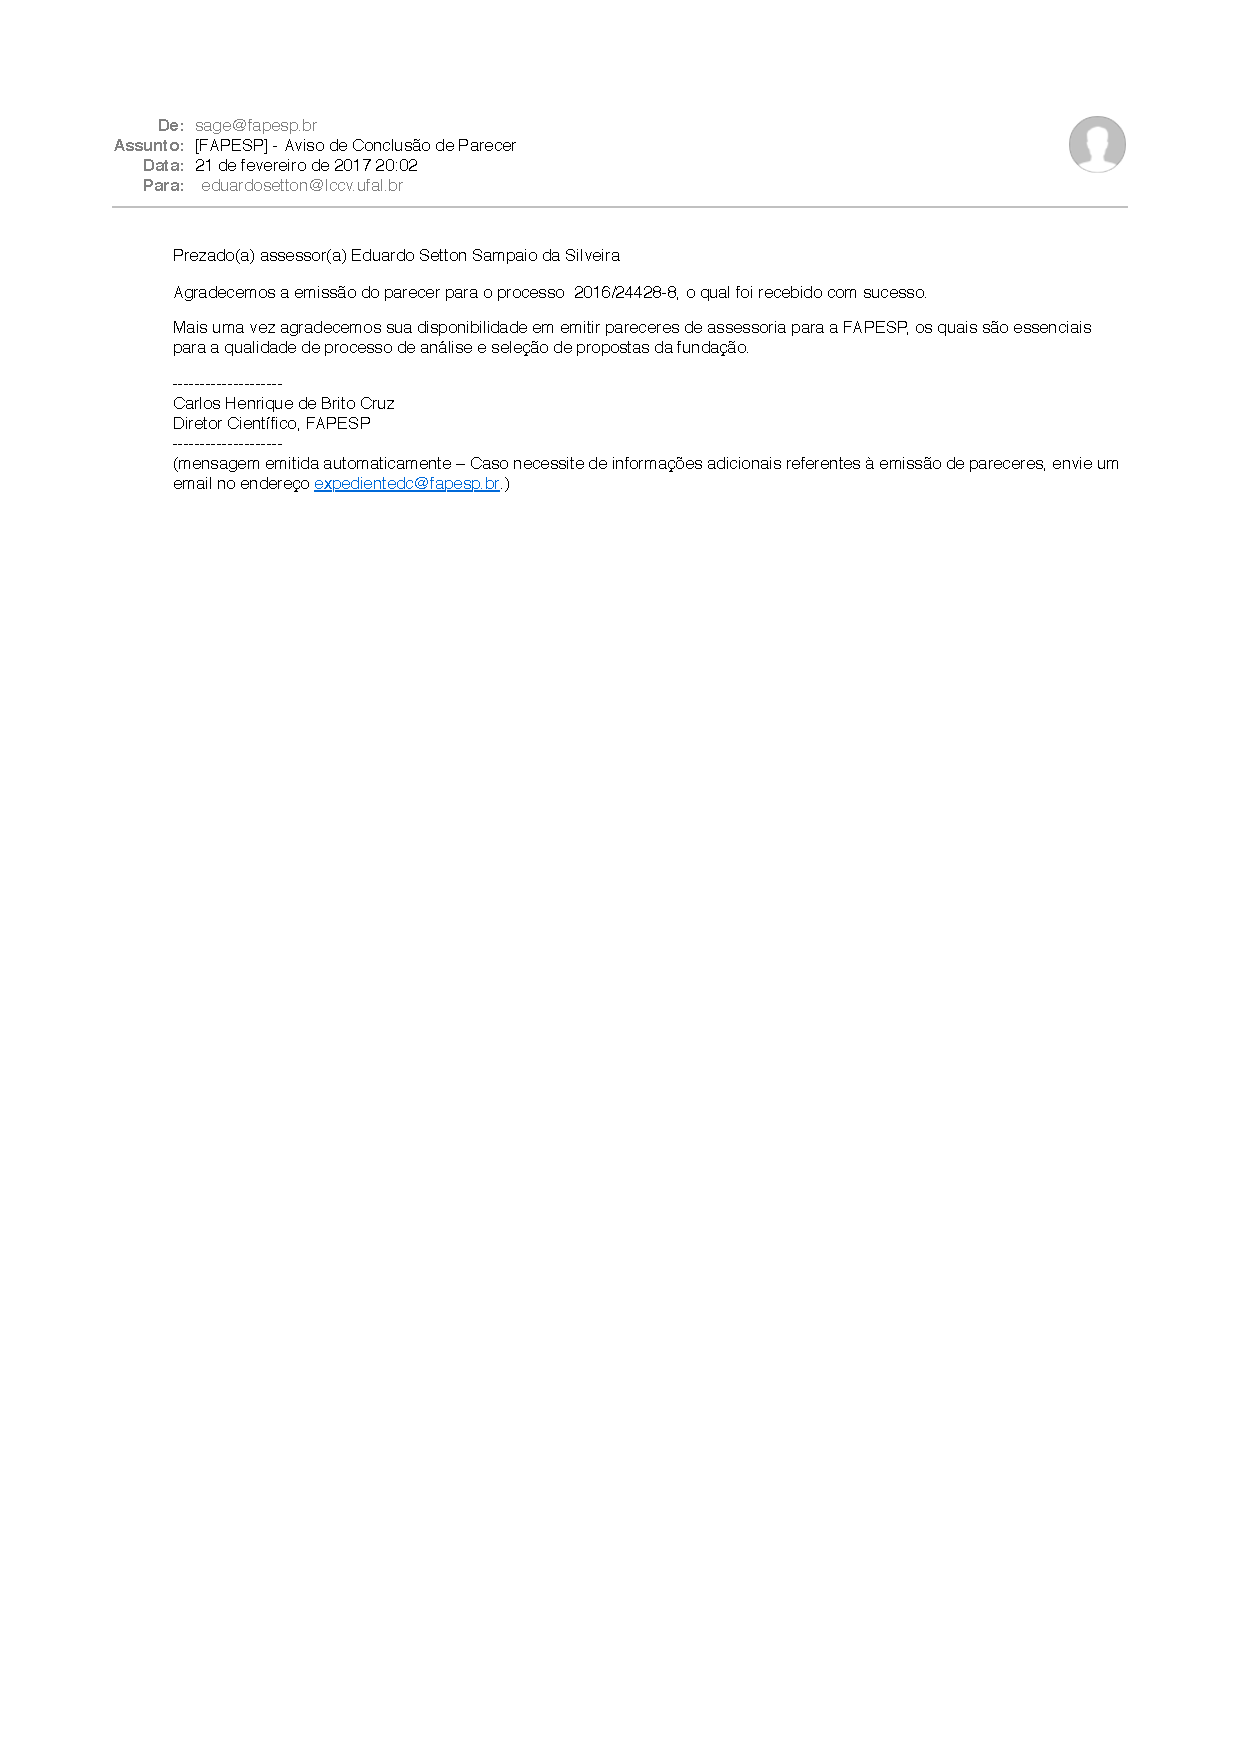
\includepdf[pages=-, scale=1, pagecommand=\thispagestyle{empty}]{\detokenize{GRUPO 2/Sub-Grupo 23/concfapesp2}}

\subsection{Parecer técnico na área de atuação do Docente}
\label{parecer:fapesp3}
Esta subseção apresenta o comprovante de atuação em Parecer técnico na área de atuação do Docente.
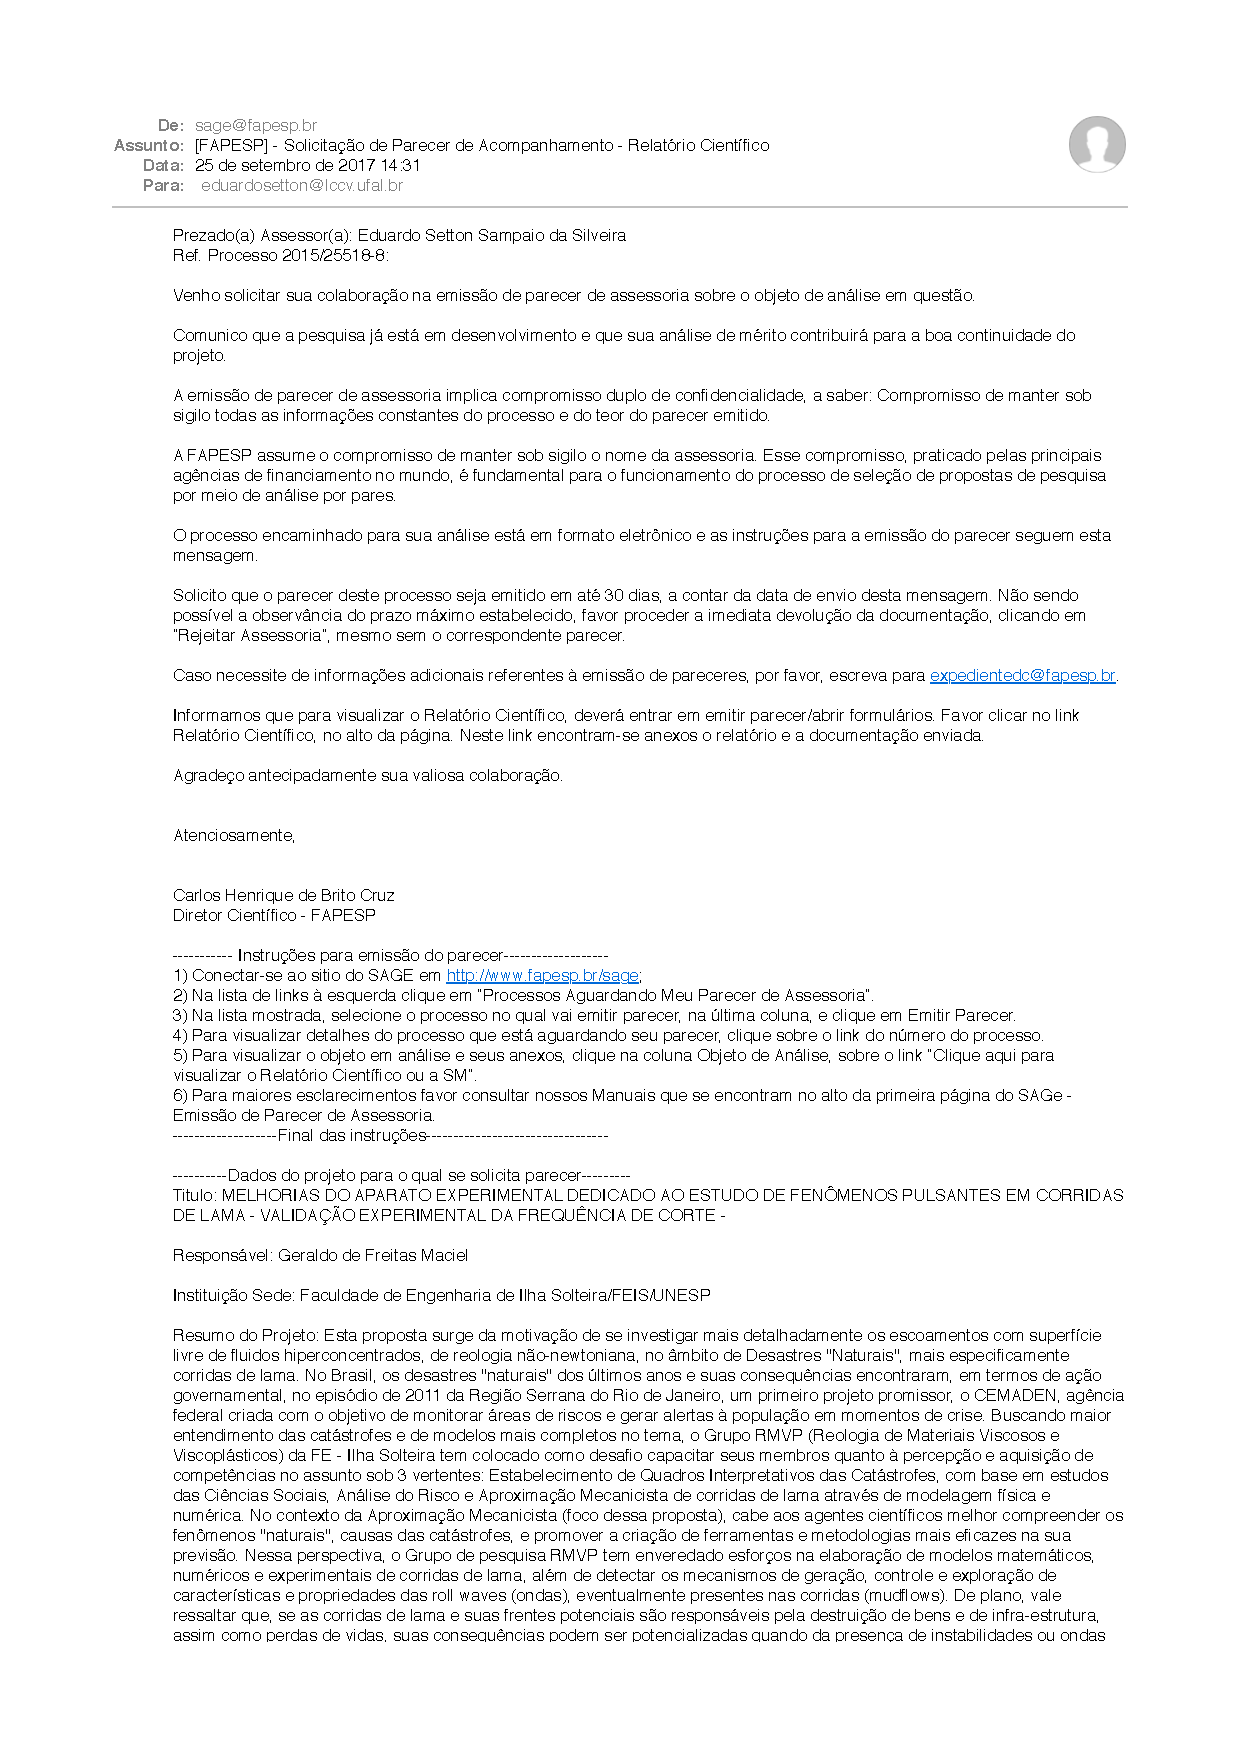
\includepdf[pages=-, scale=1, pagecommand=\thispagestyle{empty}]{\detokenize{GRUPO 2/Sub-Grupo 23/solfapesp3}}
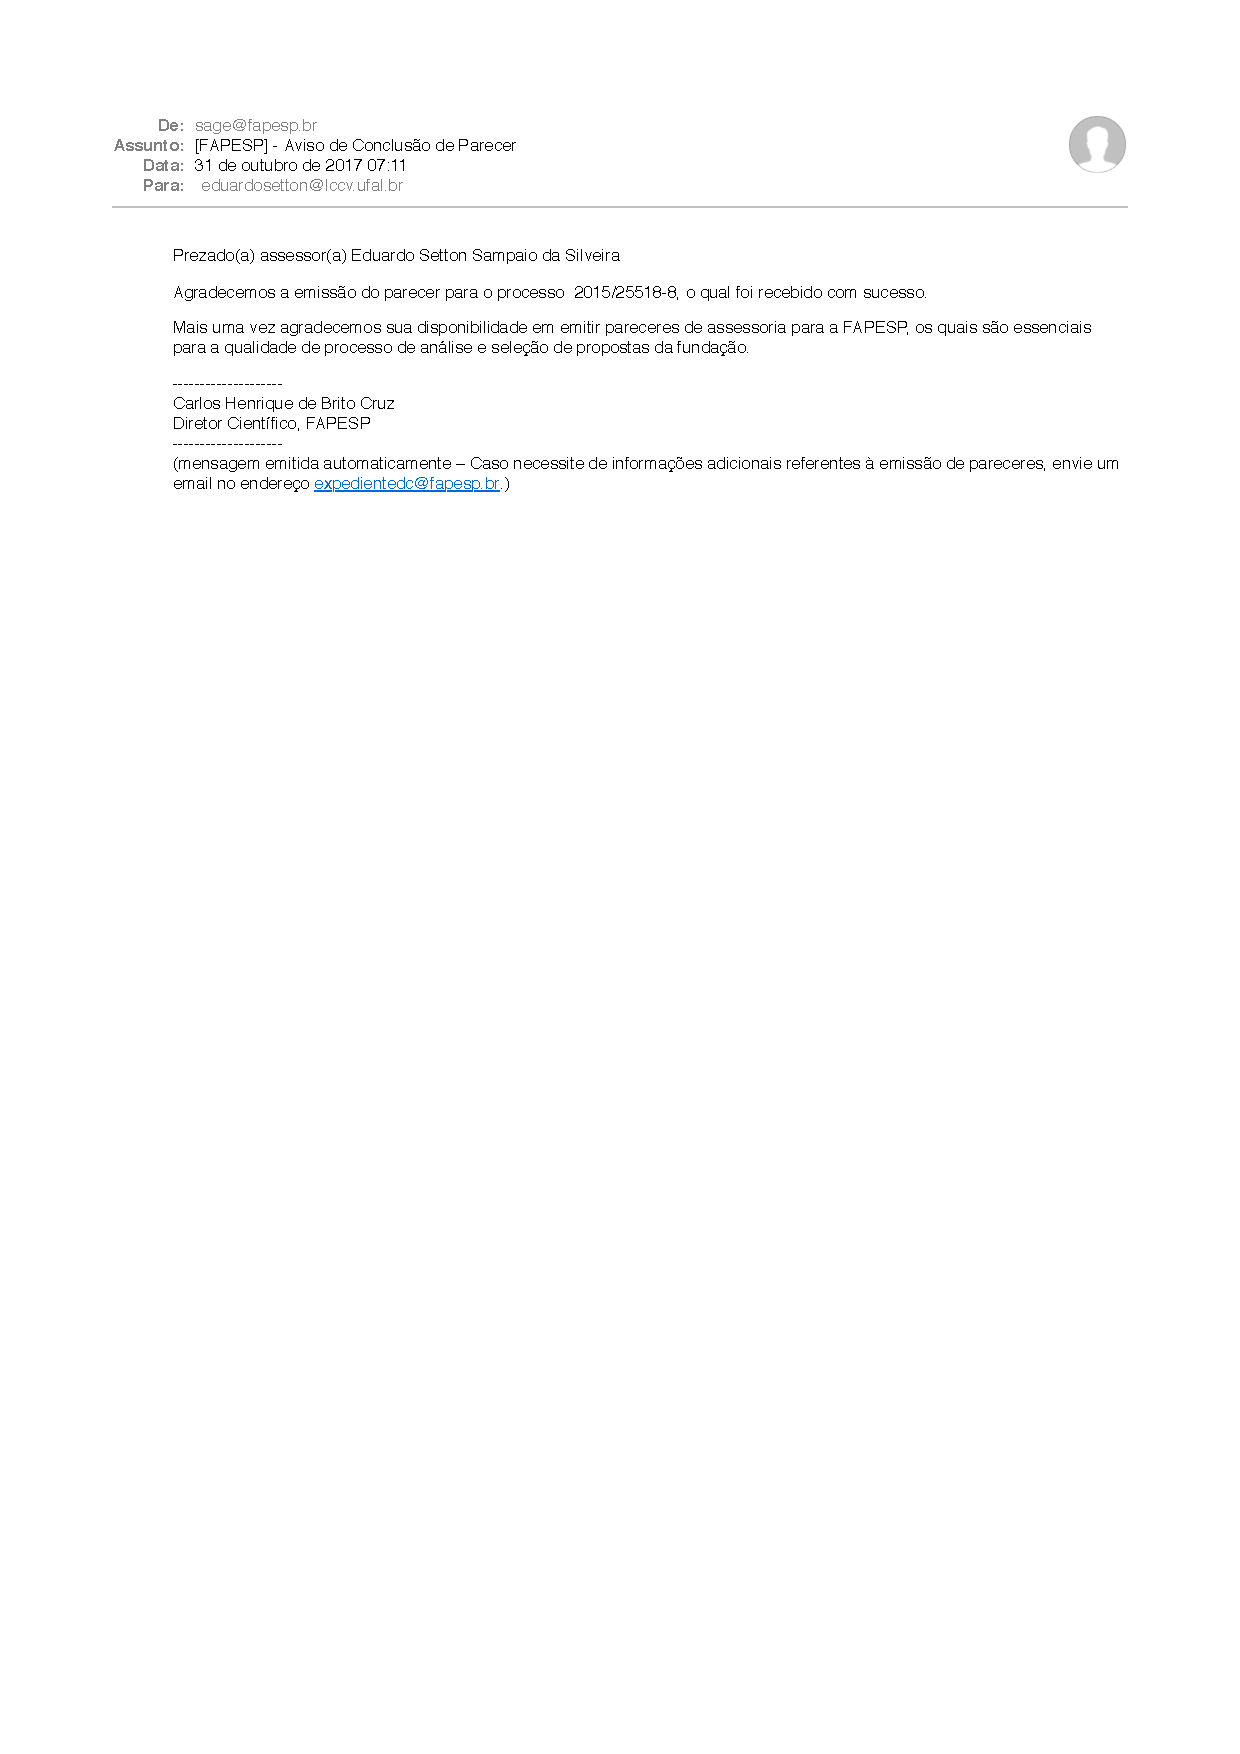
\includepdf[pages=-, scale=1, pagecommand=\thispagestyle{empty}]{\detokenize{GRUPO 2/Sub-Grupo 23/concfapesp3}}

\subsection{Parecer técnico na área de atuação do Docente}
\label{parecer:fapesp4}
Esta subseção apresenta o comprovante de atuação em Parecer técnico na área de atuação do Docente.
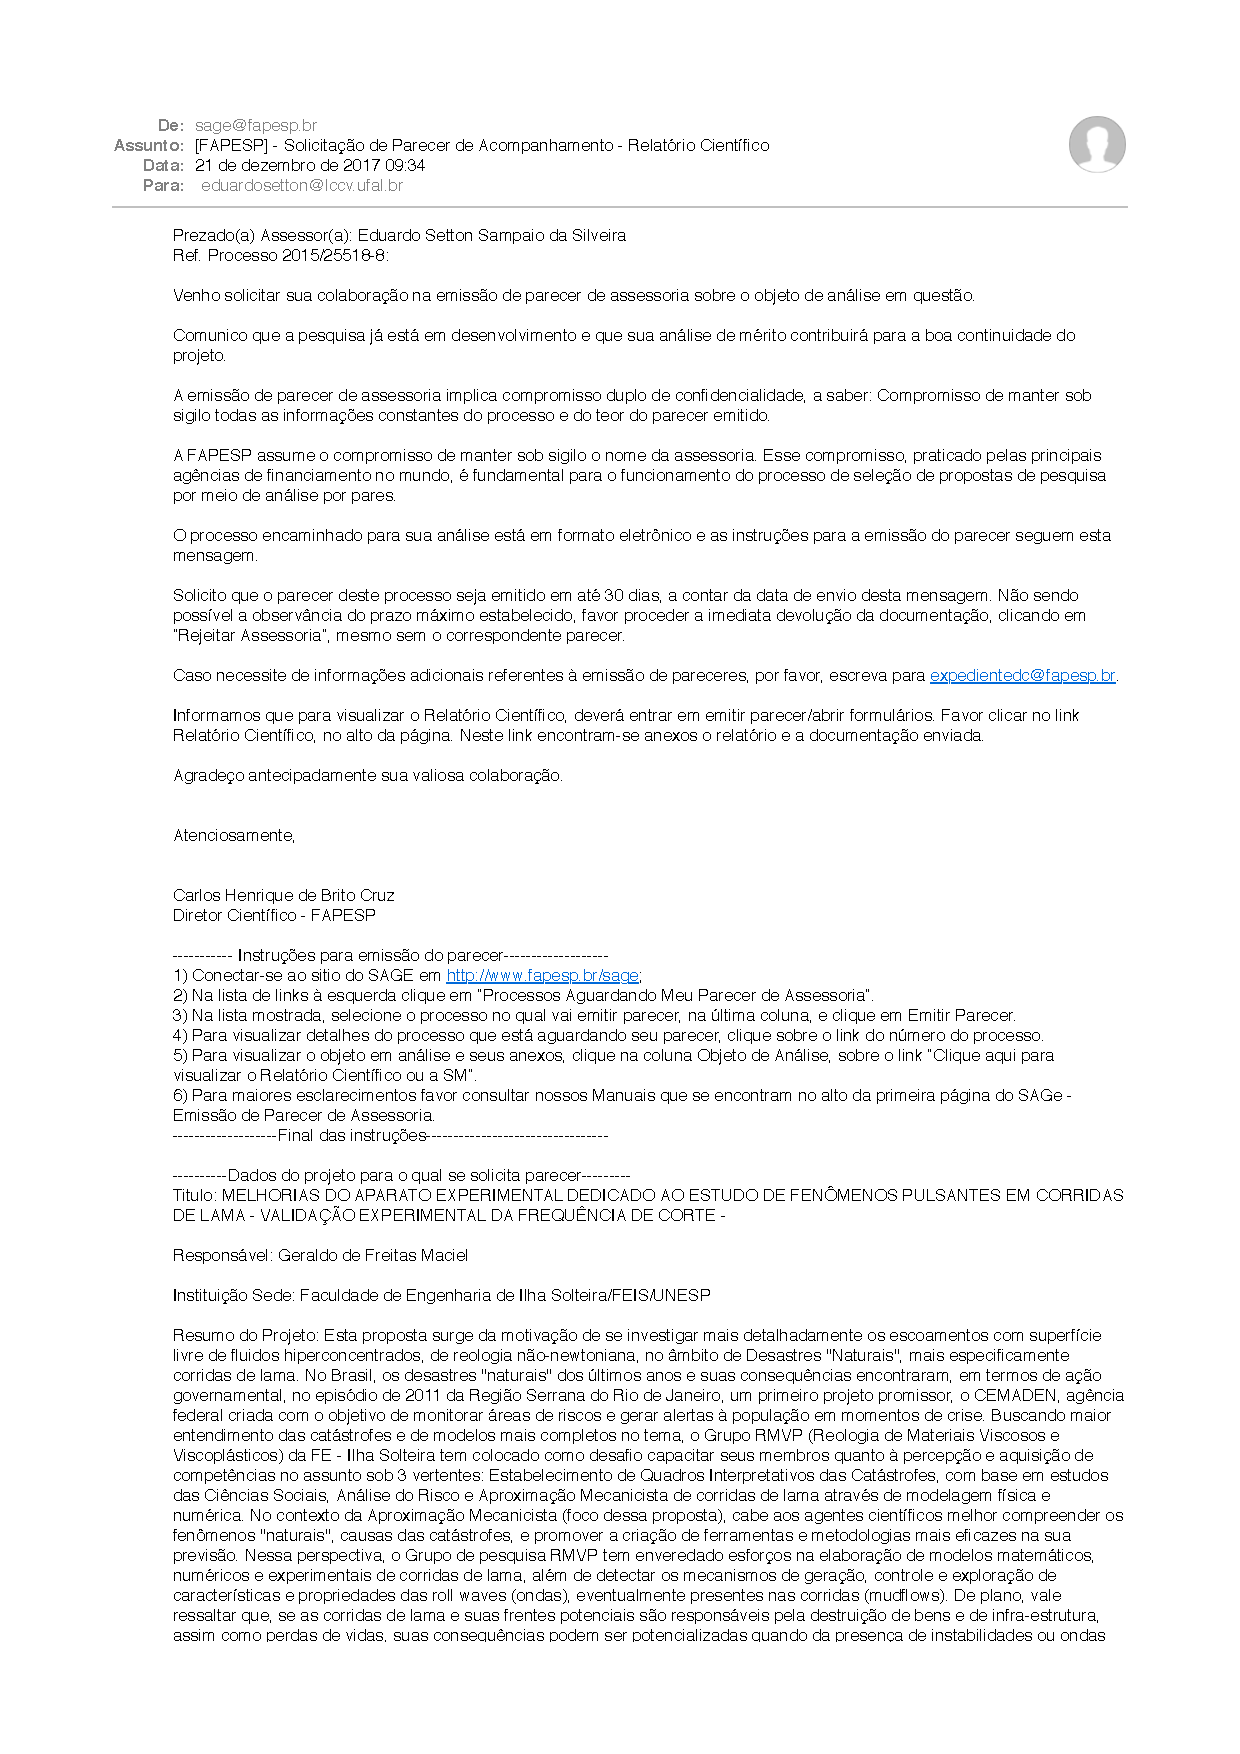
\includepdf[pages=-, scale=1, pagecommand=\thispagestyle{empty}]{\detokenize{GRUPO 2/Sub-Grupo 23/solfapesp4}}
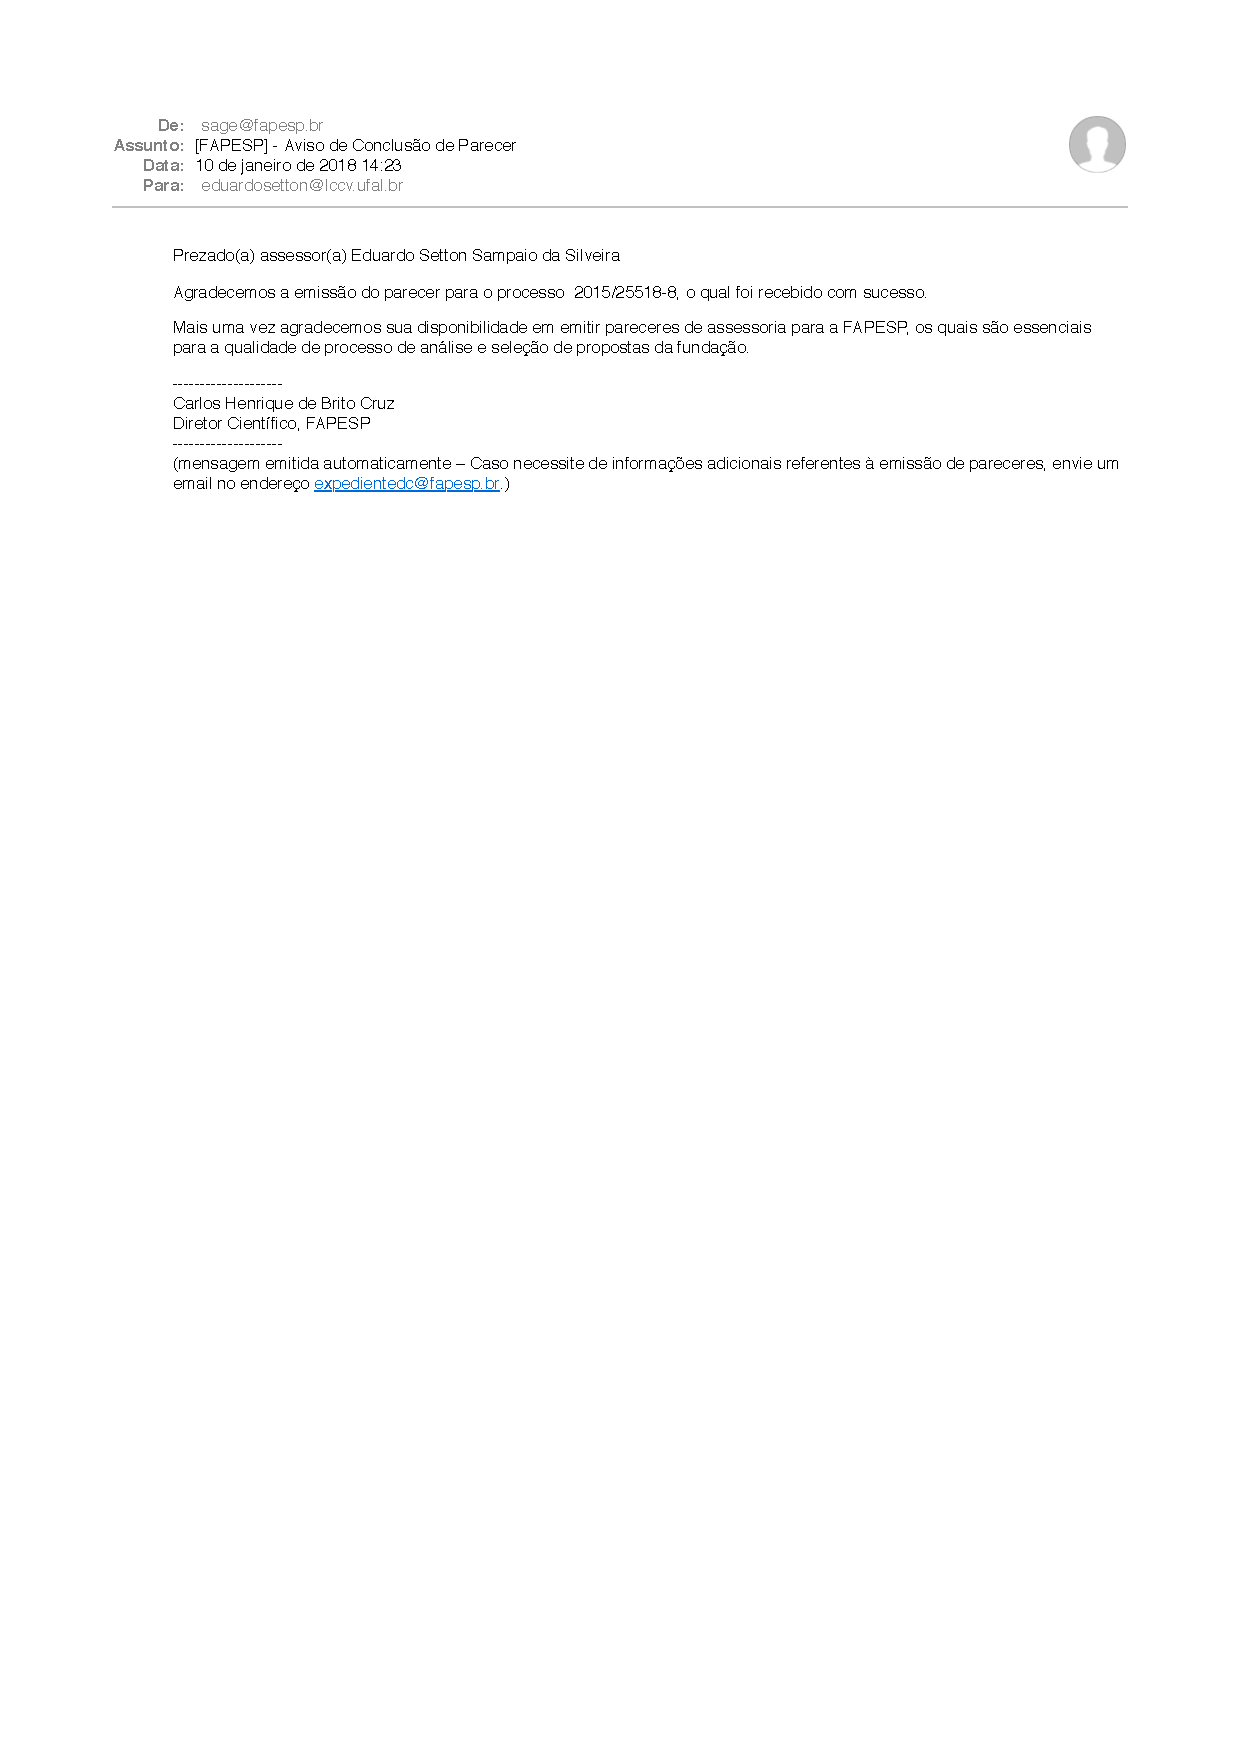
\includepdf[pages=-, scale=1, pagecommand=\thispagestyle{empty}]{\detokenize{GRUPO 2/Sub-Grupo 23/concfapesp4}}


%%%%%%%%%%%%%%%%%%%%%%%%%%%%%%%%%%%%%%%%%%%%%%%%%%%%%%%%%%%%%%%%%%%%%%%%%%%%%%%
% Subgrupo 2.4 - Parecer Técnico
%%%%%%%%%%%%%%%%%%%%%%%%%%%%%%%%%%%%%%%%%%%%%%%%%%%%%%%%%%%%%%%%%%%%%%%%%%%%%%%
\subsection{Artigo completo publicado em anais de congressos evento internacional}
\label{conf:2017-artigoprospecti}
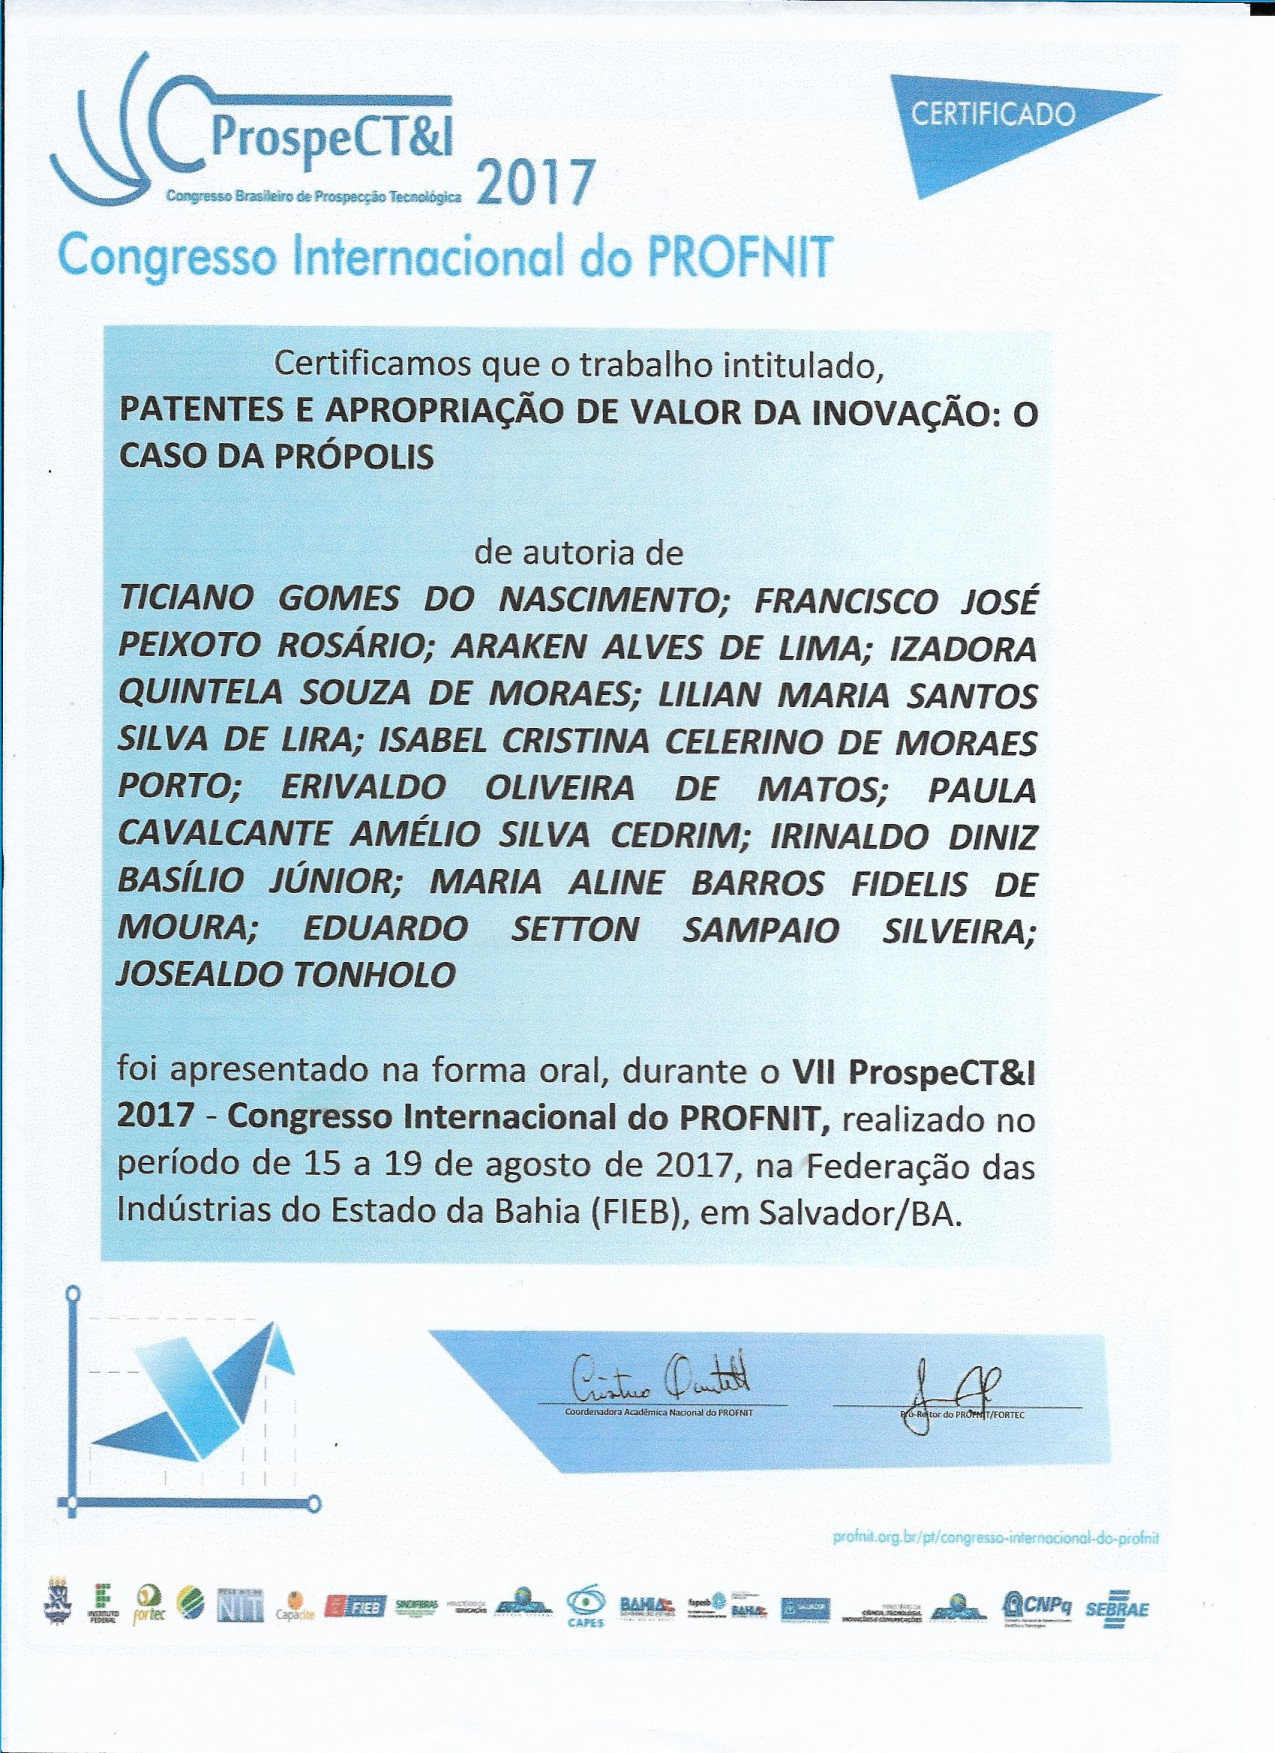
\includepdf[pages=-, scale=1, pagecommand=\thispagestyle{empty}]{\detokenize{GRUPO 2/Sub-Grupo 24/2017-artigoprospecti}}

\subsection{Artigo completo publicado em anais de congressos evento internacional}
\label{conf:2017-artigocilamce}
Esta subseção apresenta o comprovante da publicação de Artigo completo publicado em anais de congressos evento internacional.
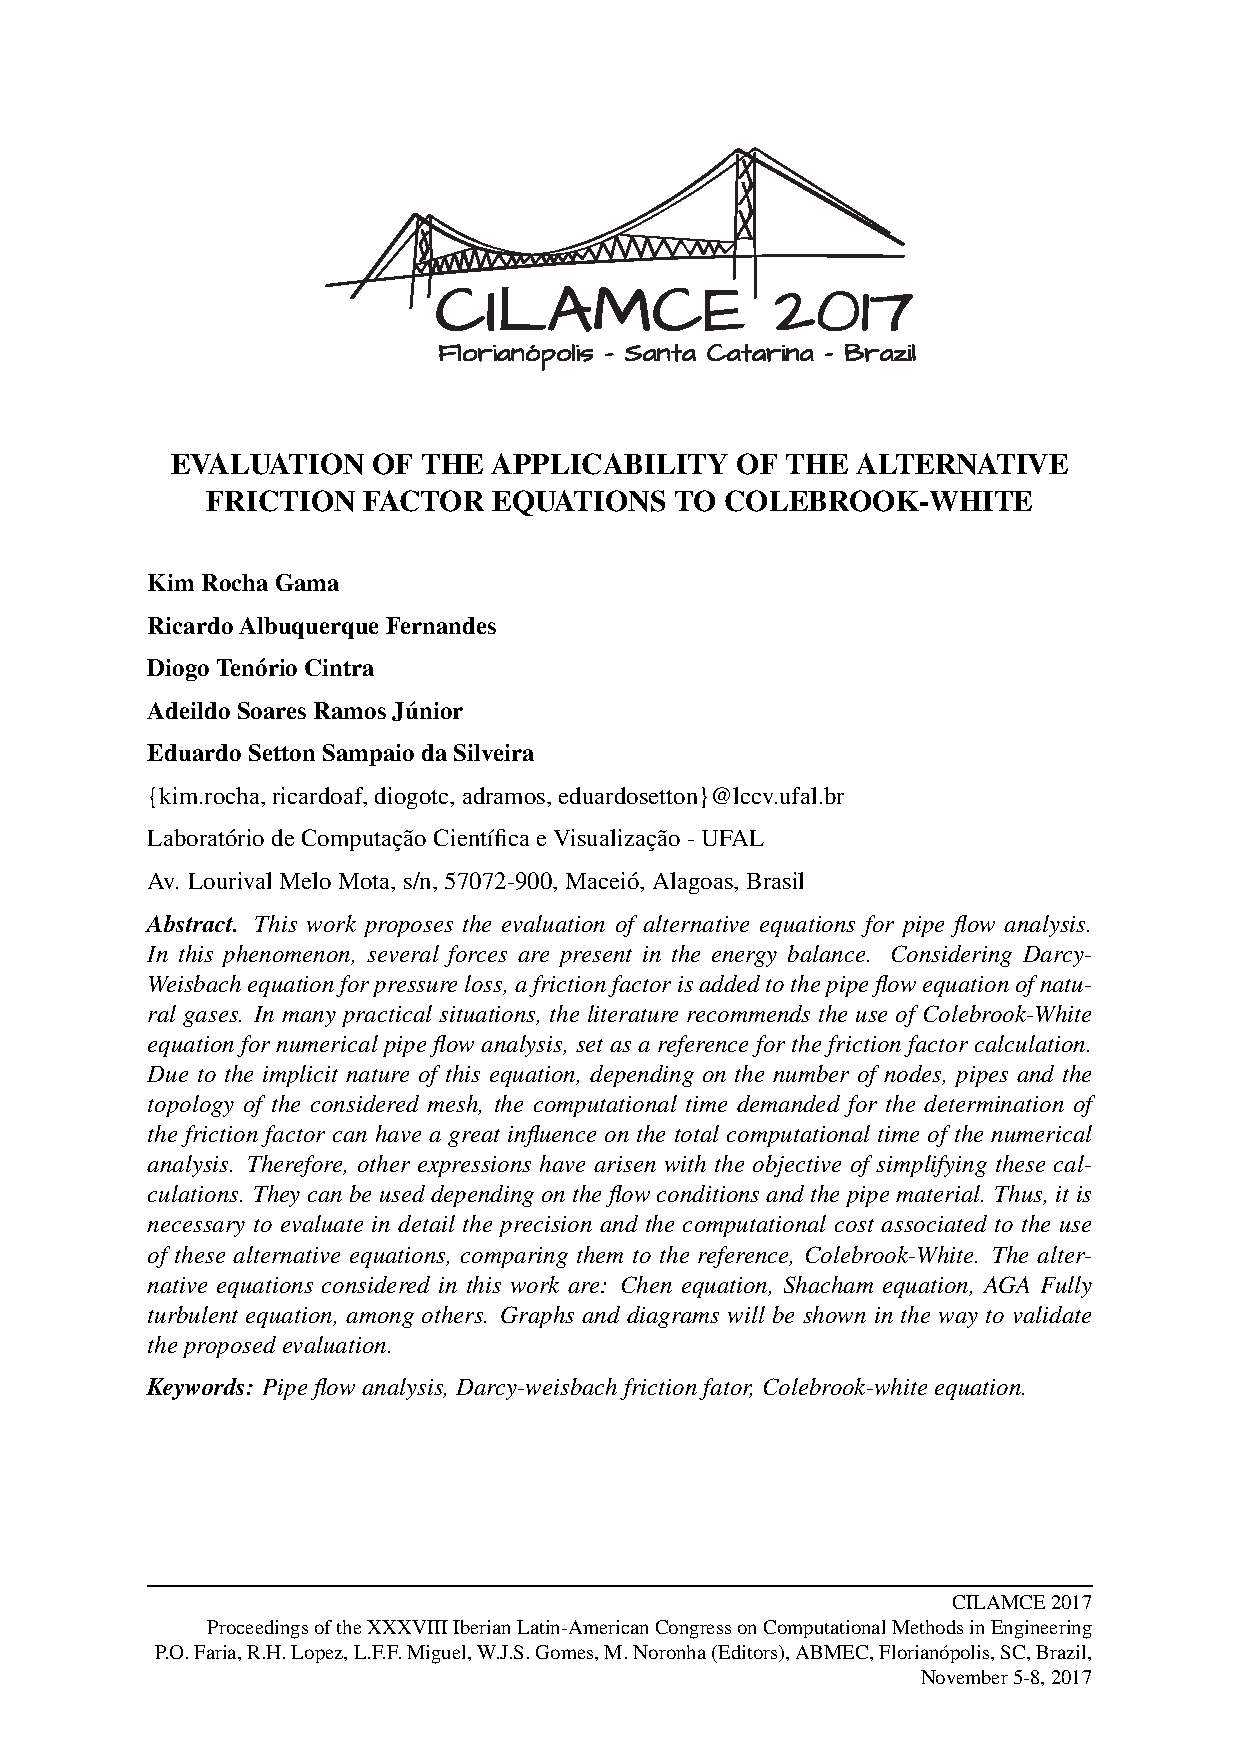
\includepdf[pages=-, scale=1, pagecommand=\thispagestyle{empty}]{\detokenize{GRUPO 2/Sub-Grupo 24/2017-artigocilamce}}

\subsection{Artigo completo publicado em anais de congressos evento nacional ou regional}
\label{artigo:2016-artigocobenge}
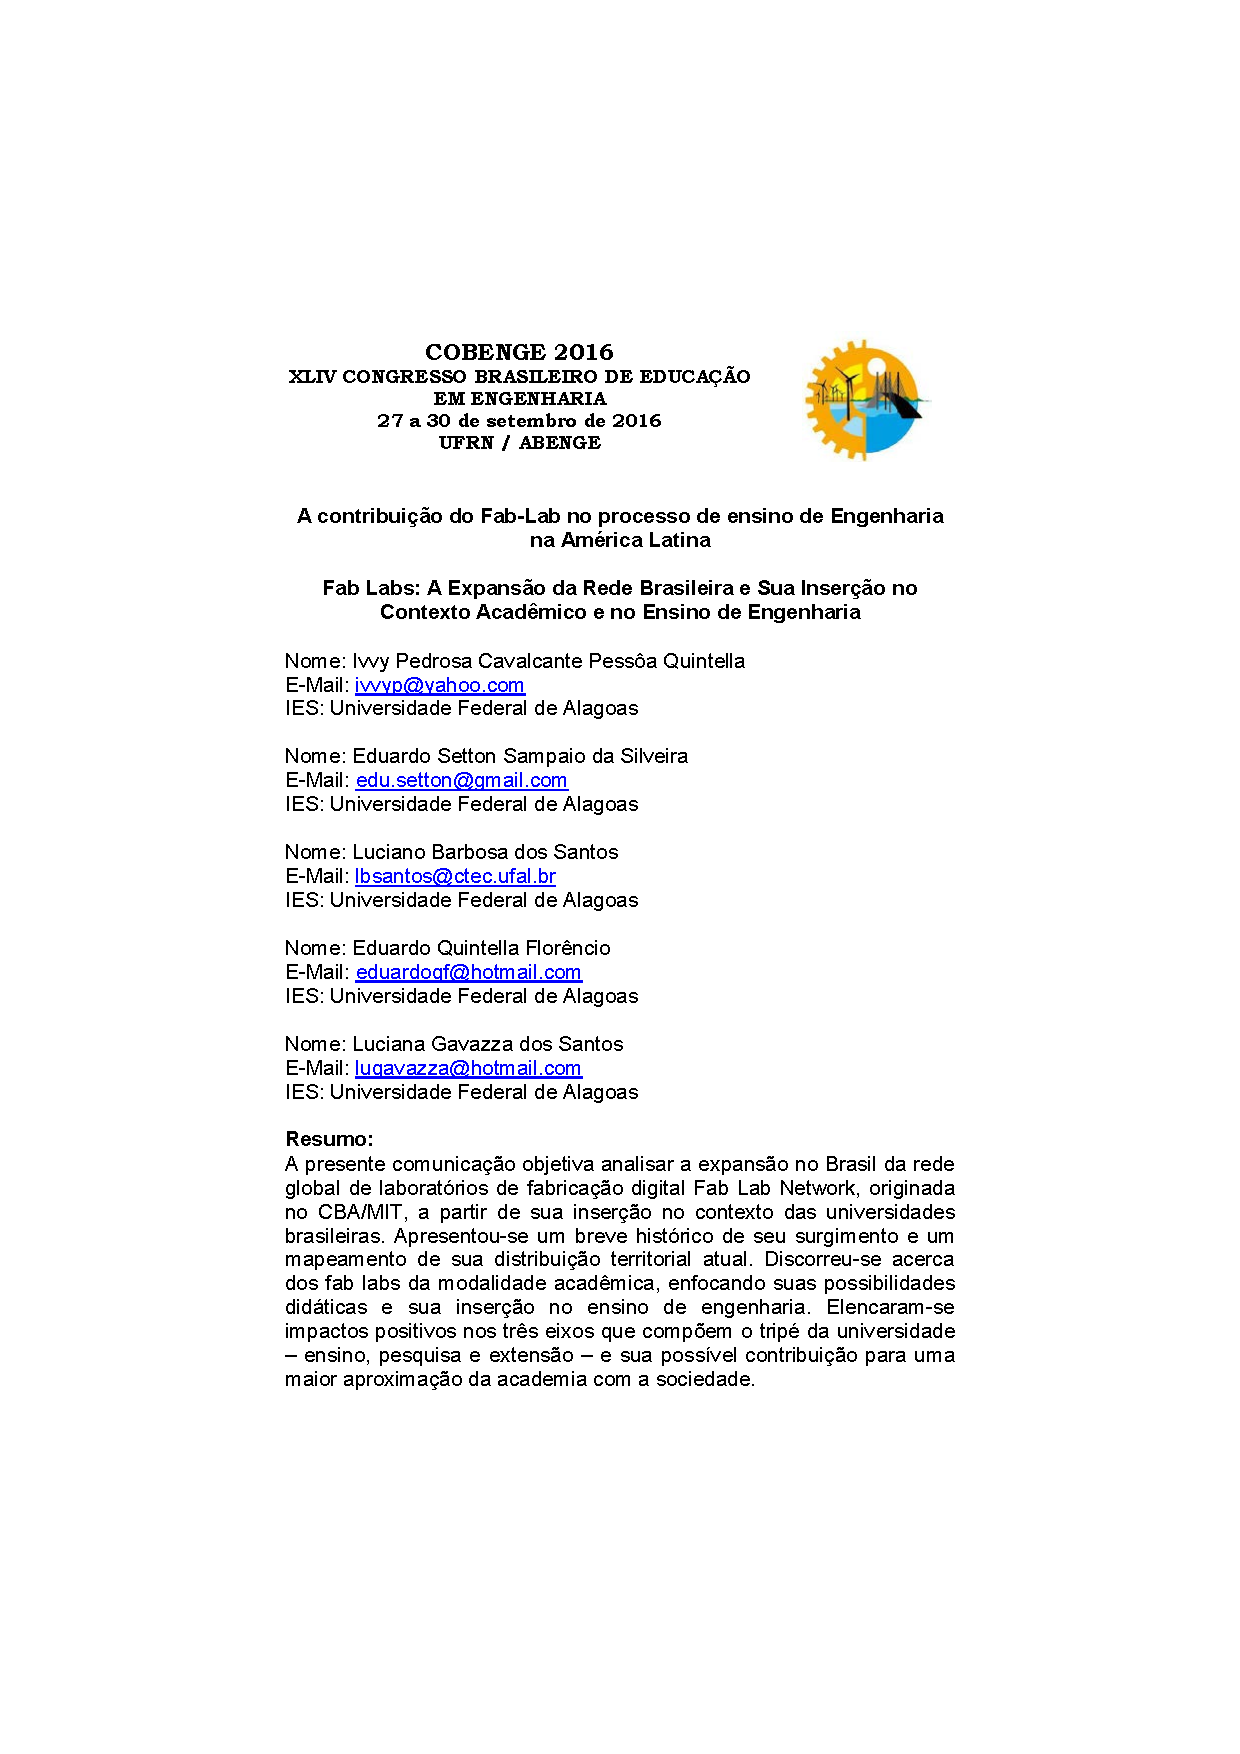
\includepdf[pages=-, scale=1, pagecommand=\thispagestyle{empty}]{\detokenize{GRUPO 2/Sub-Grupo 24/2016-artigocobenge}}

\subsection{Artigo completo publicado em anais de congressos evento nacional ou regional}
\label{artigo:2016-artigoanprotec}
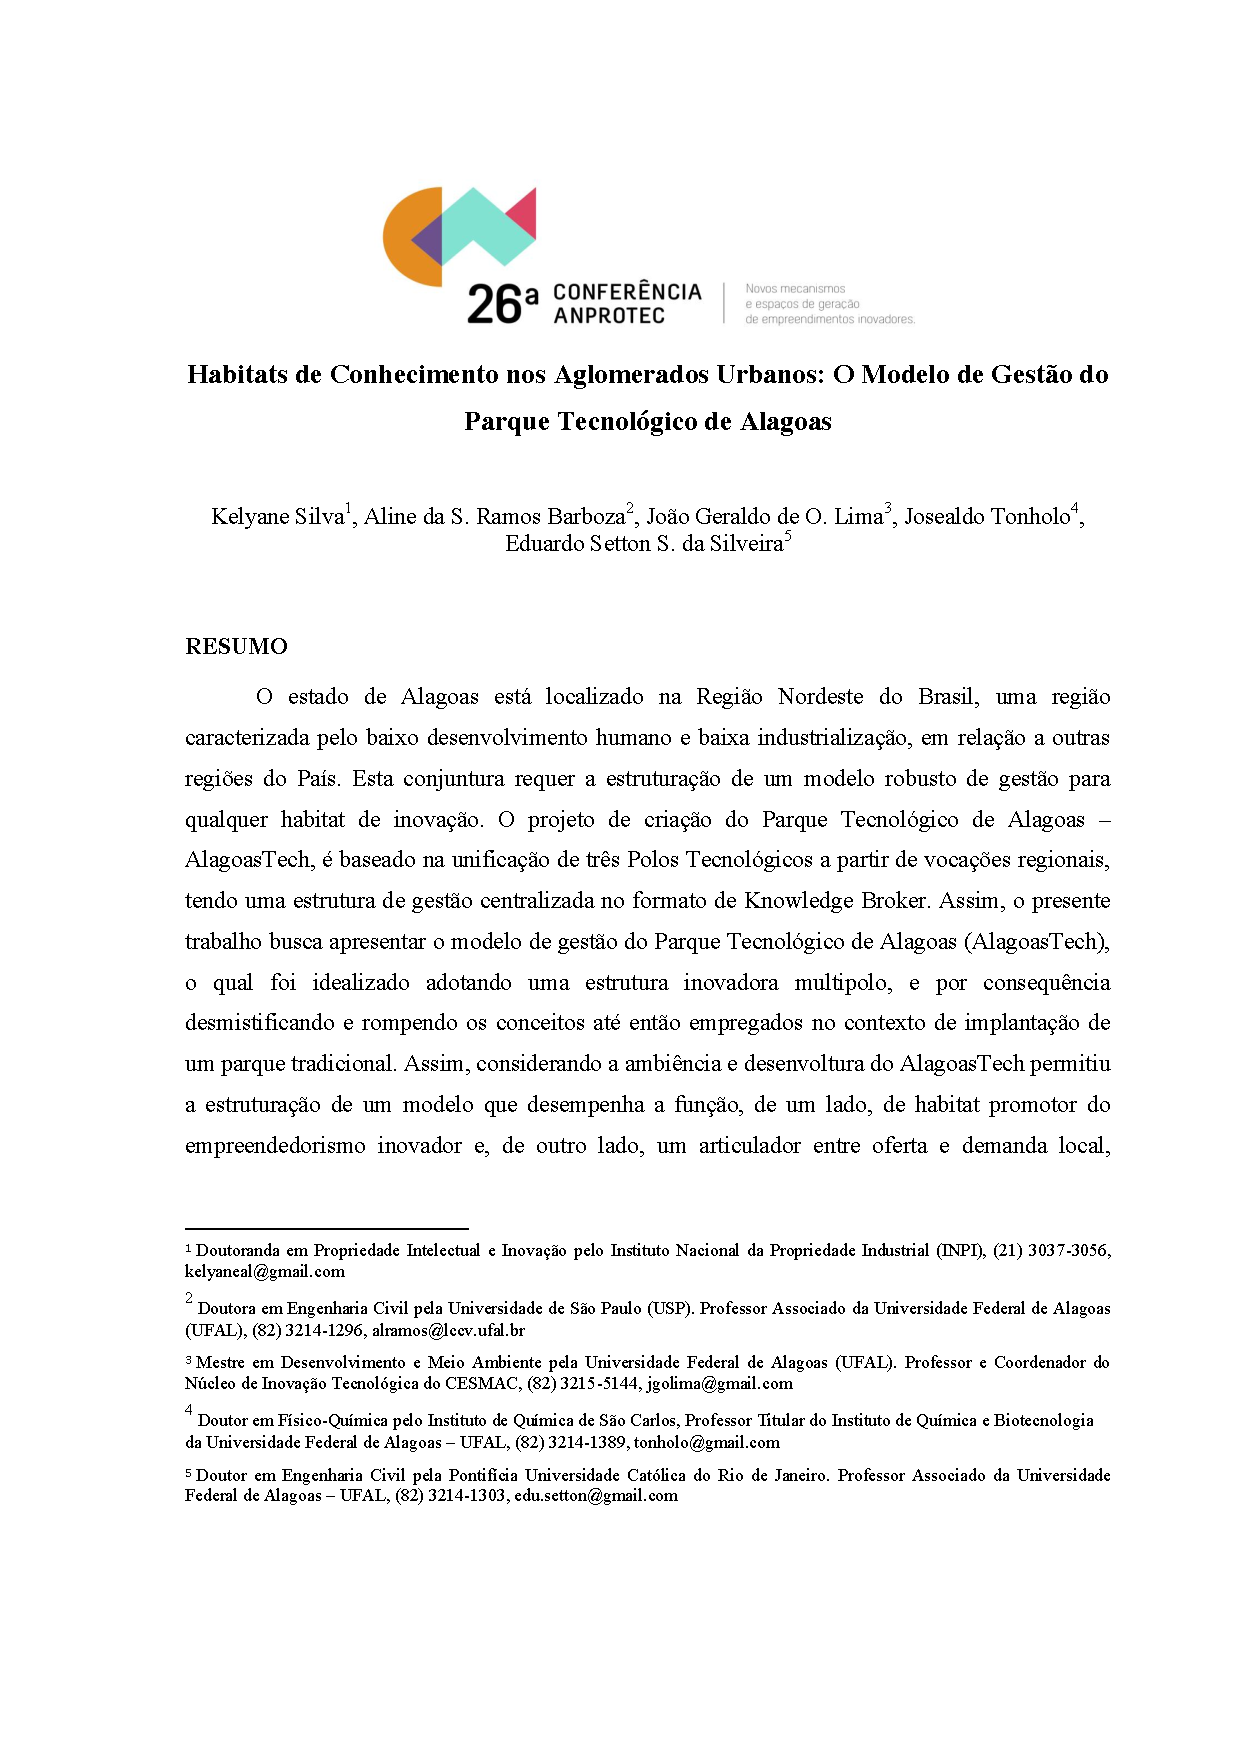
\includepdf[pages=-, scale=1, pagecommand=\thispagestyle{empty}]{\detokenize{GRUPO 2/Sub-Grupo 24/2016-artigoanprotec}}

\subsection{Artigo completo publicado em anais de congressos evento nacional ou regional}
\label{artigo:2017-artigopdpetro1}
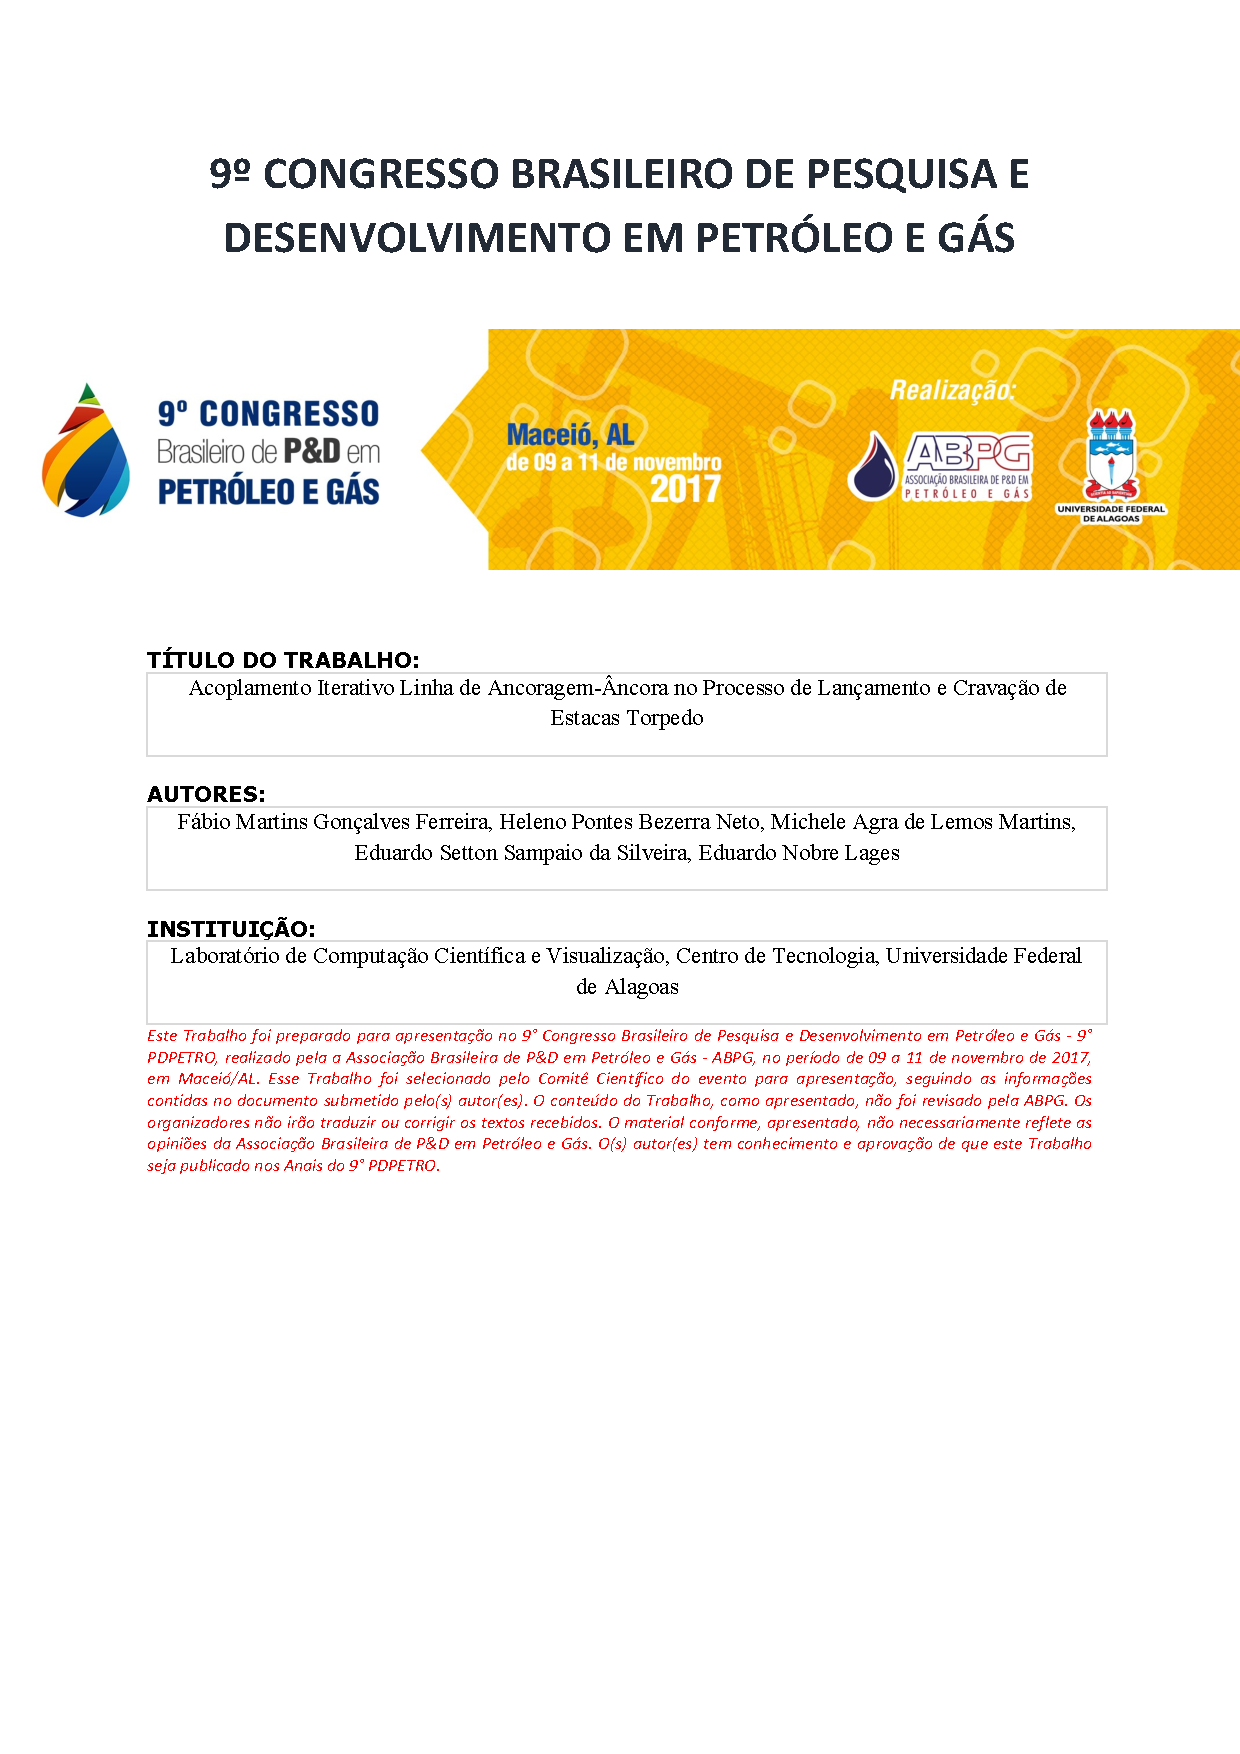
\includepdf[pages=-, scale=1, pagecommand=\thispagestyle{empty}]{\detokenize{GRUPO 2/Sub-Grupo 24/2017-artigopdpetro1}}

\subsection{Artigo completo publicado em anais de congressos evento nacional ou regional}
\label{artigo:2017-artigopdpetro2}
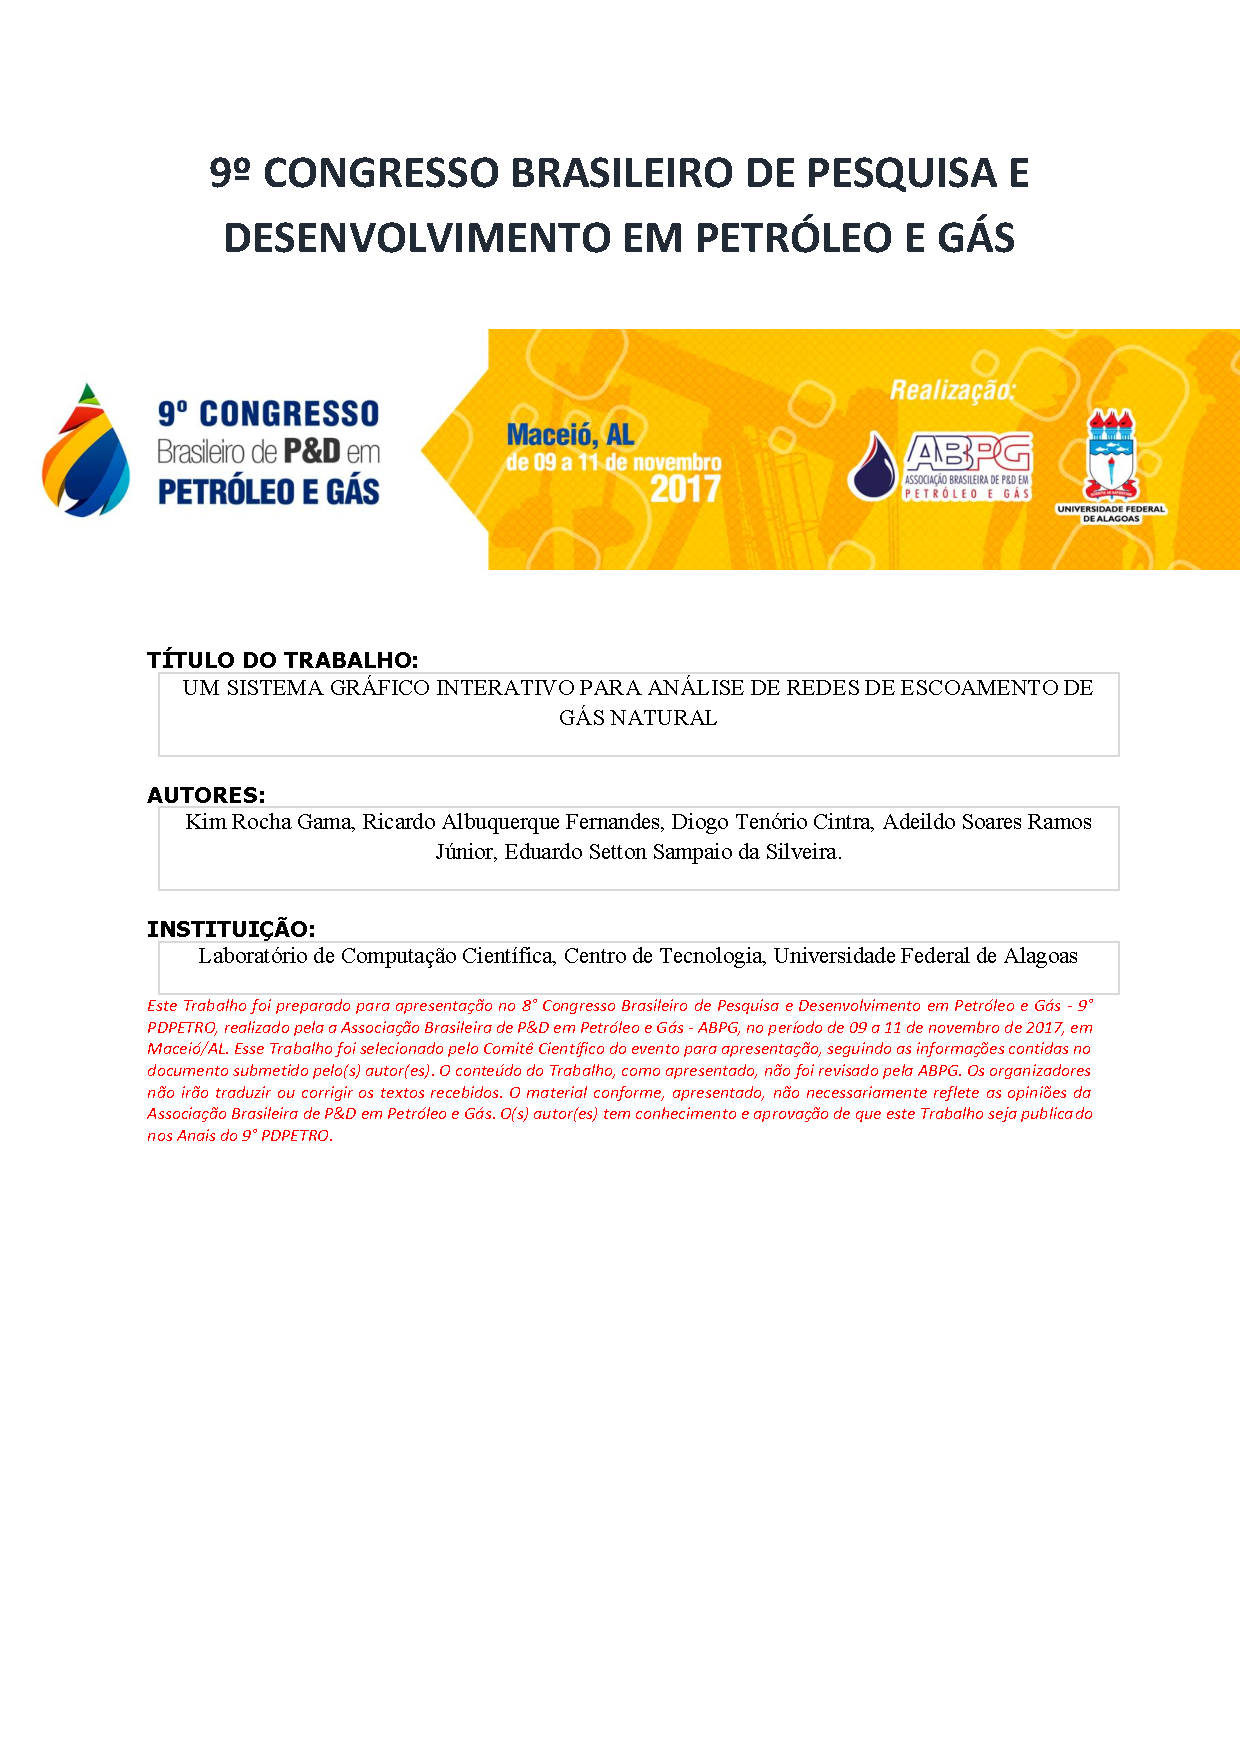
\includepdf[pages=-, scale=1, pagecommand=\thispagestyle{empty}]{\detokenize{GRUPO 2/Sub-Grupo 24/2017-artigopdpetro2}}

\subsection{Artigo completo publicado em anais de congressos evento nacional ou regional}
\label{artigo:2017-artigopdpetro3}
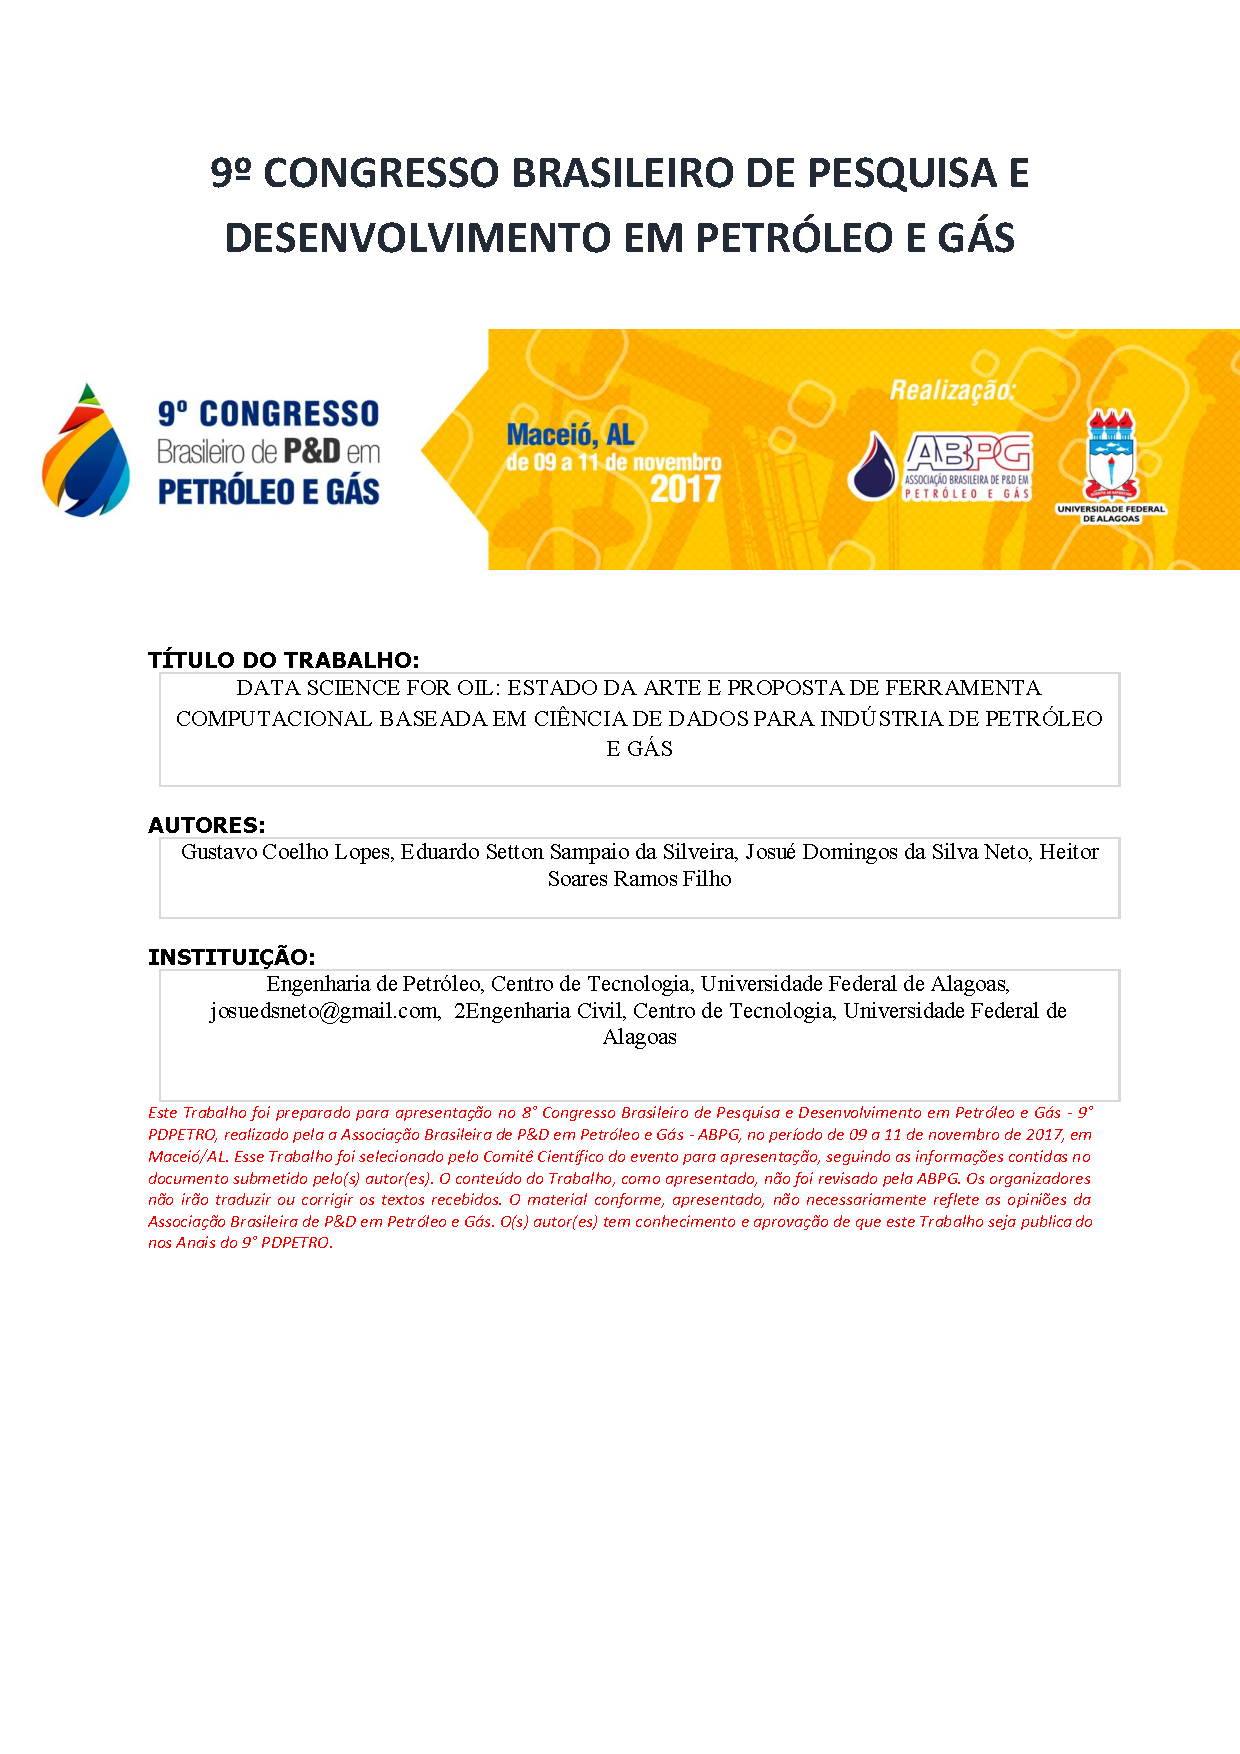
\includepdf[pages=-, scale=1, pagecommand=\thispagestyle{empty}]{\detokenize{GRUPO 2/Sub-Grupo 24/2017-artigopdpetro3}}

\subsection{Artigo completo publicado em anais de congressos evento nacional ou regional}
\label{artigo:2017-artigopdpetro4}
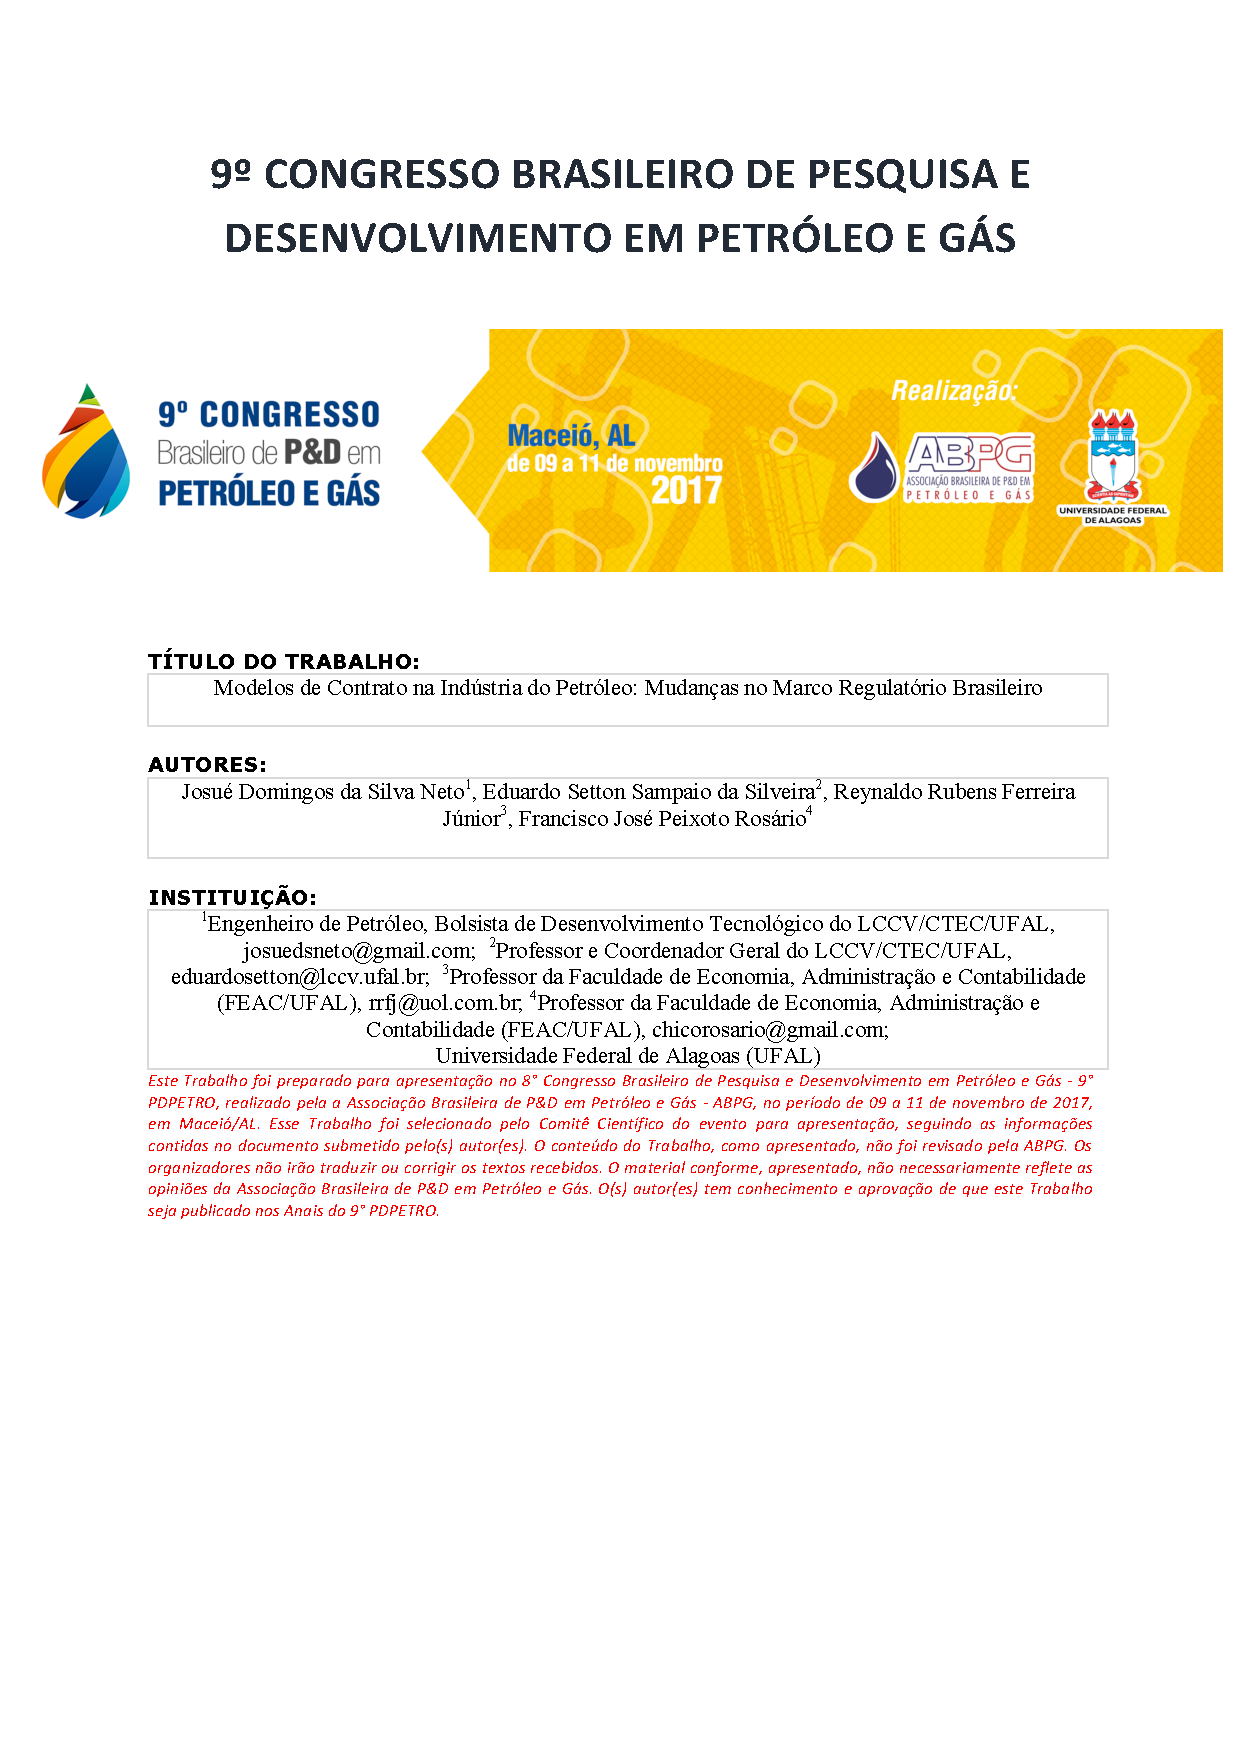
\includepdf[pages=-, scale=1, pagecommand=\thispagestyle{empty}]{\detokenize{GRUPO 2/Sub-Grupo 24/2017-artigopdpetro4}}

\subsection{Artigo completo publicado em anais de congressos evento nacional ou regional}
\label{artigo:2017-artigopdpetro5}
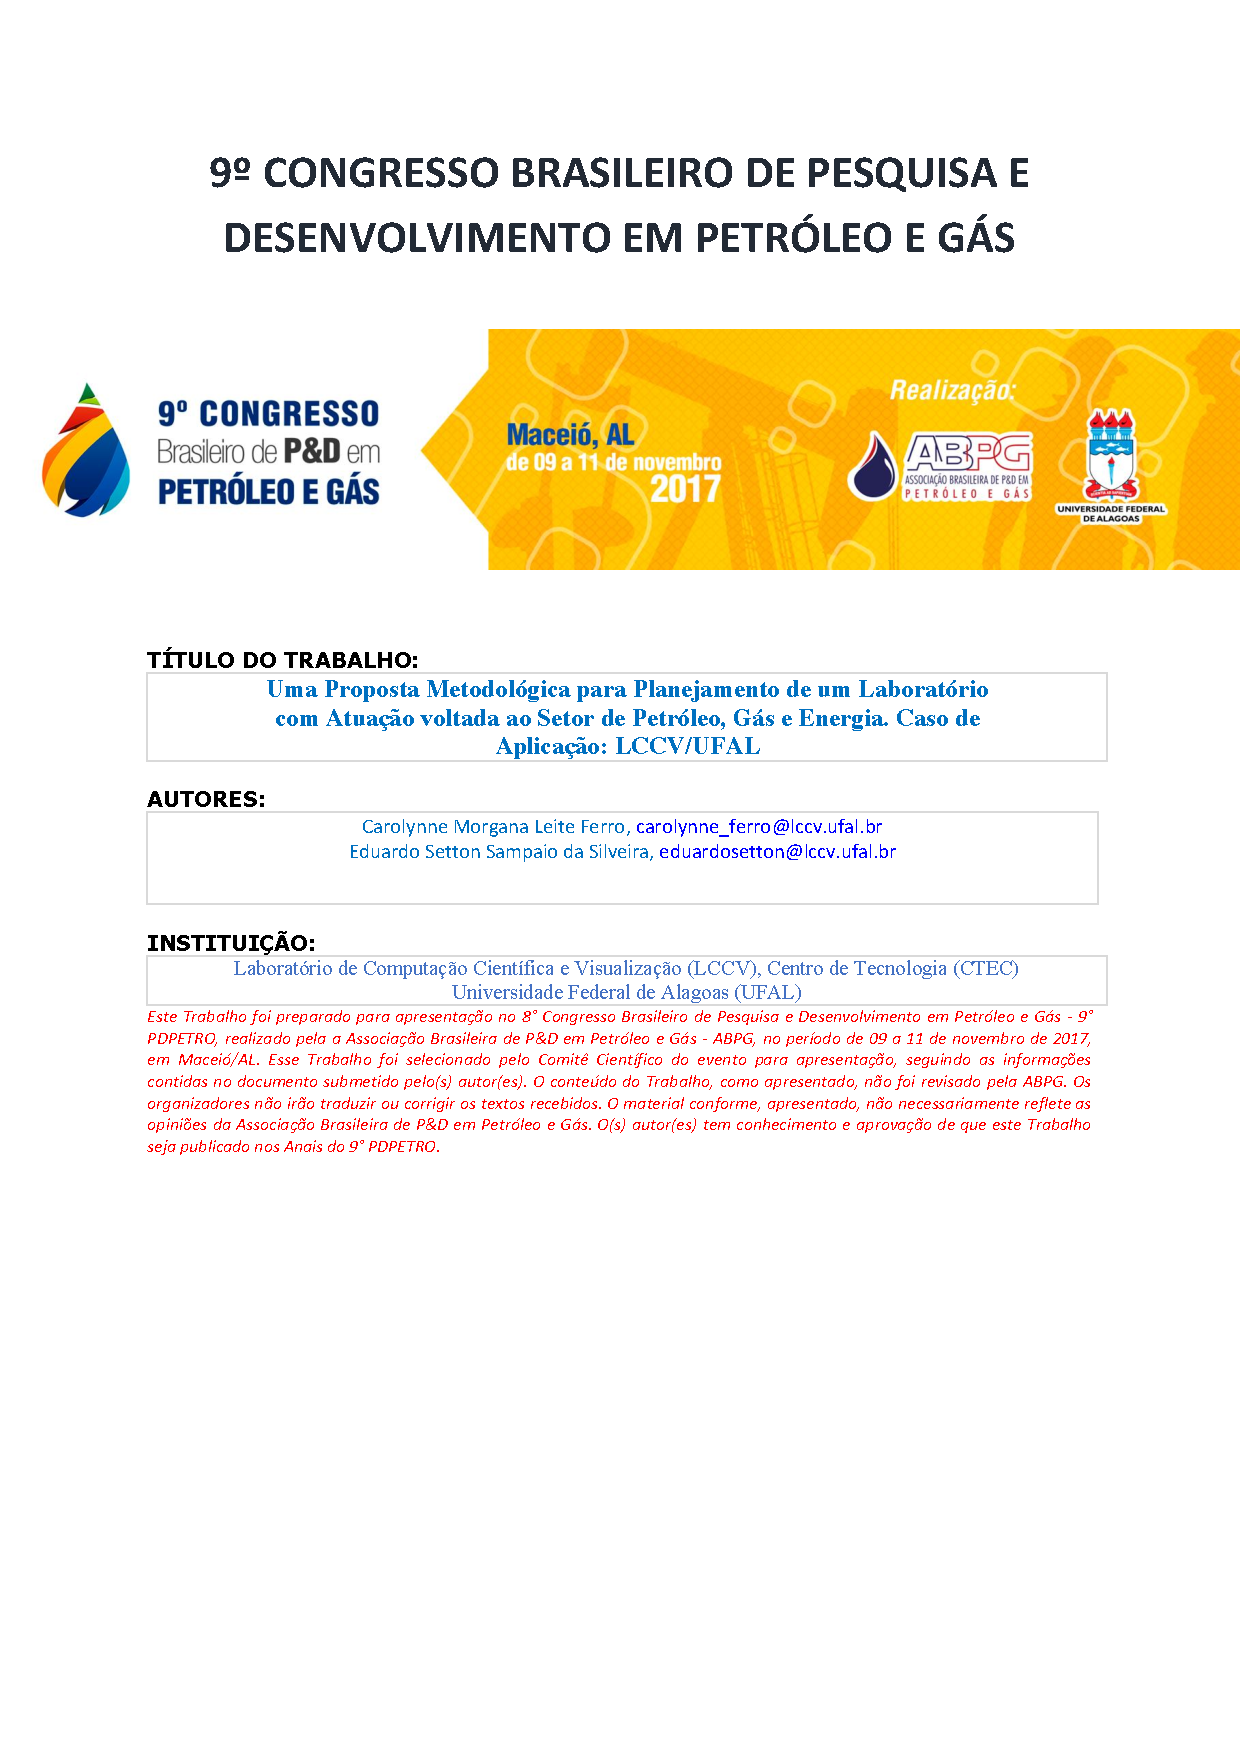
\includepdf[pages=-, scale=1, pagecommand=\thispagestyle{empty}]{\detokenize{GRUPO 2/Sub-Grupo 24/2017-artigopdpetro5}}

\subsection{Participação em eventos científicos, profissionais ou artísticos com apresentação oral de trabalho em evento nacional ou regional}
\label{app:2017-apppdpetro}
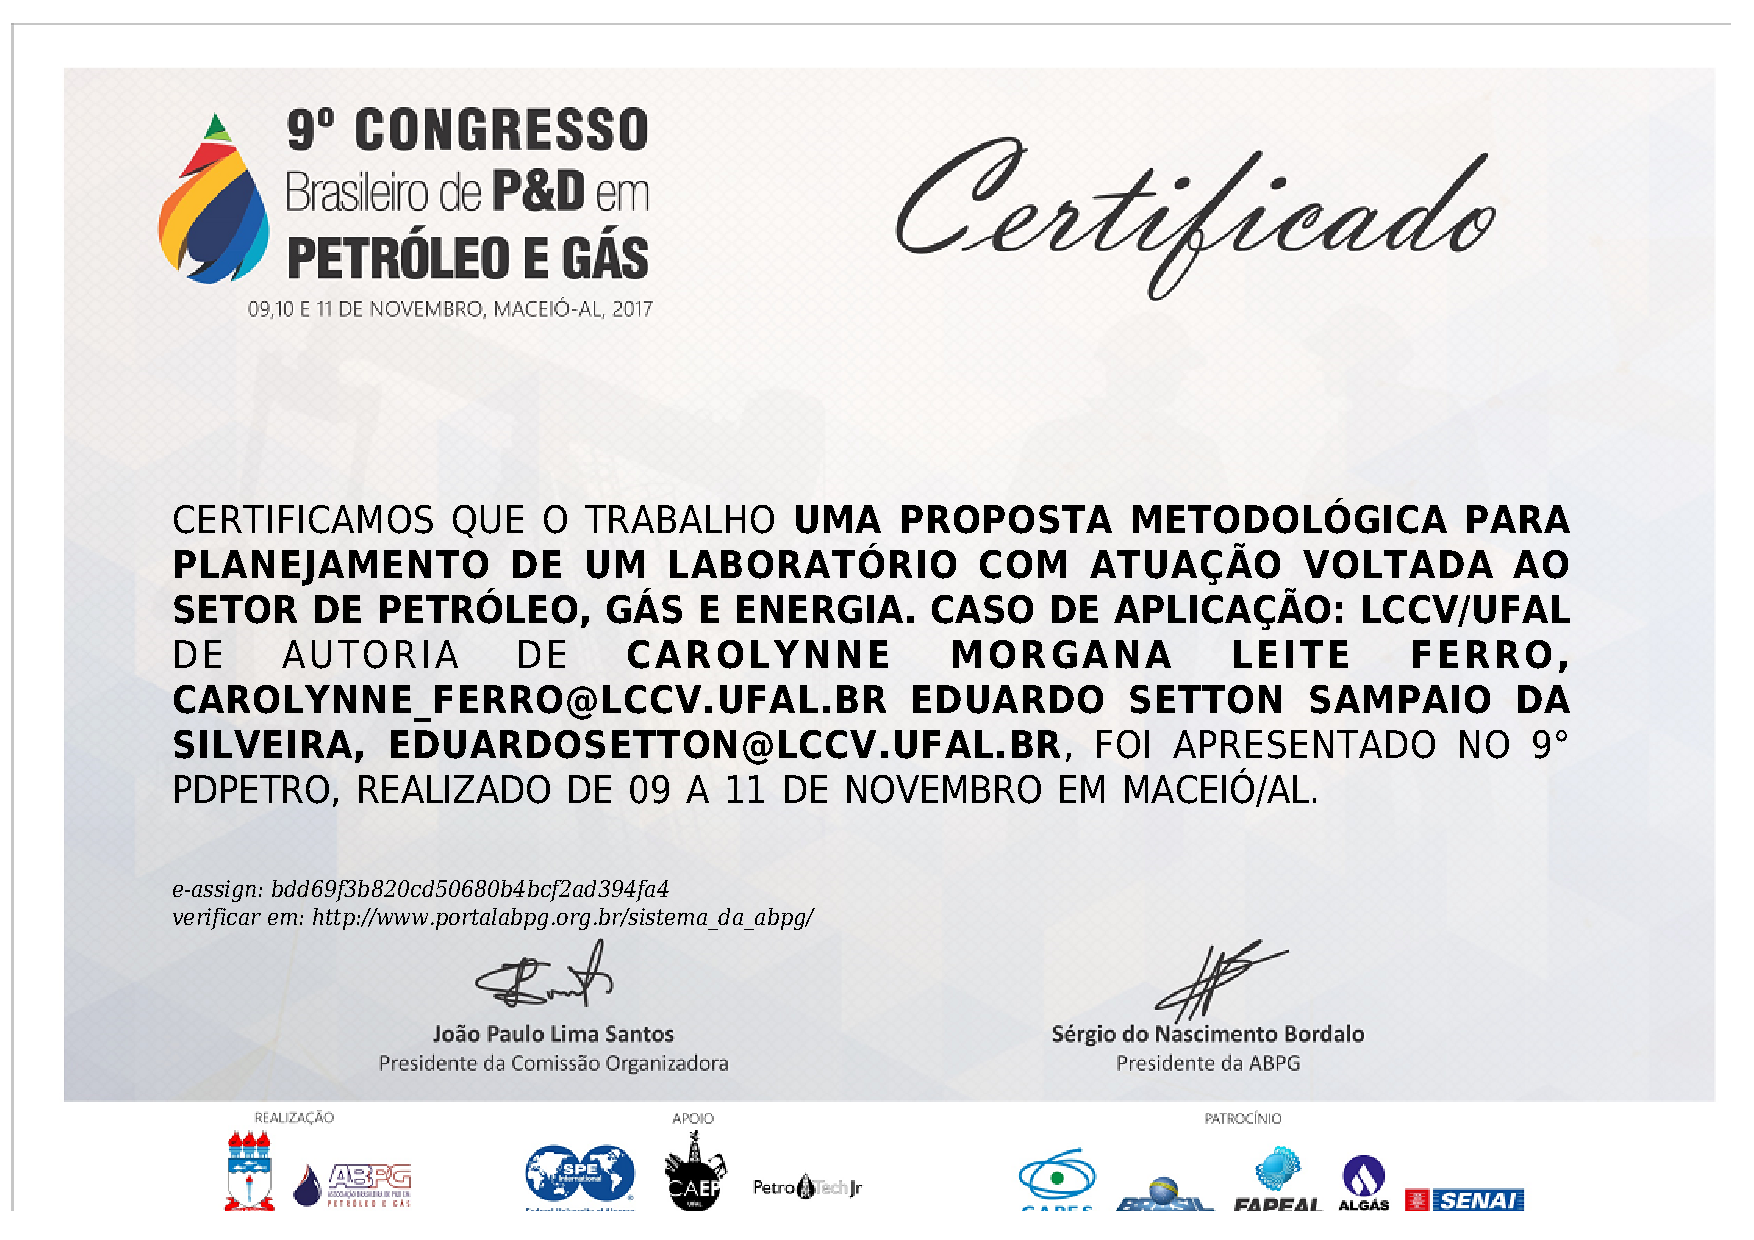
\includepdf[pages=-, scale=1, pagecommand=\thispagestyle{empty}]{\detokenize{GRUPO 2/Sub-Grupo 25/2017-apppdpetro}}

\subsection{Participação em eventos científicos, profissionais ou artísticos sem apresentação oral de trabalho em evento nacional ou regional}
\label{app:2017-inovarpconstruir}
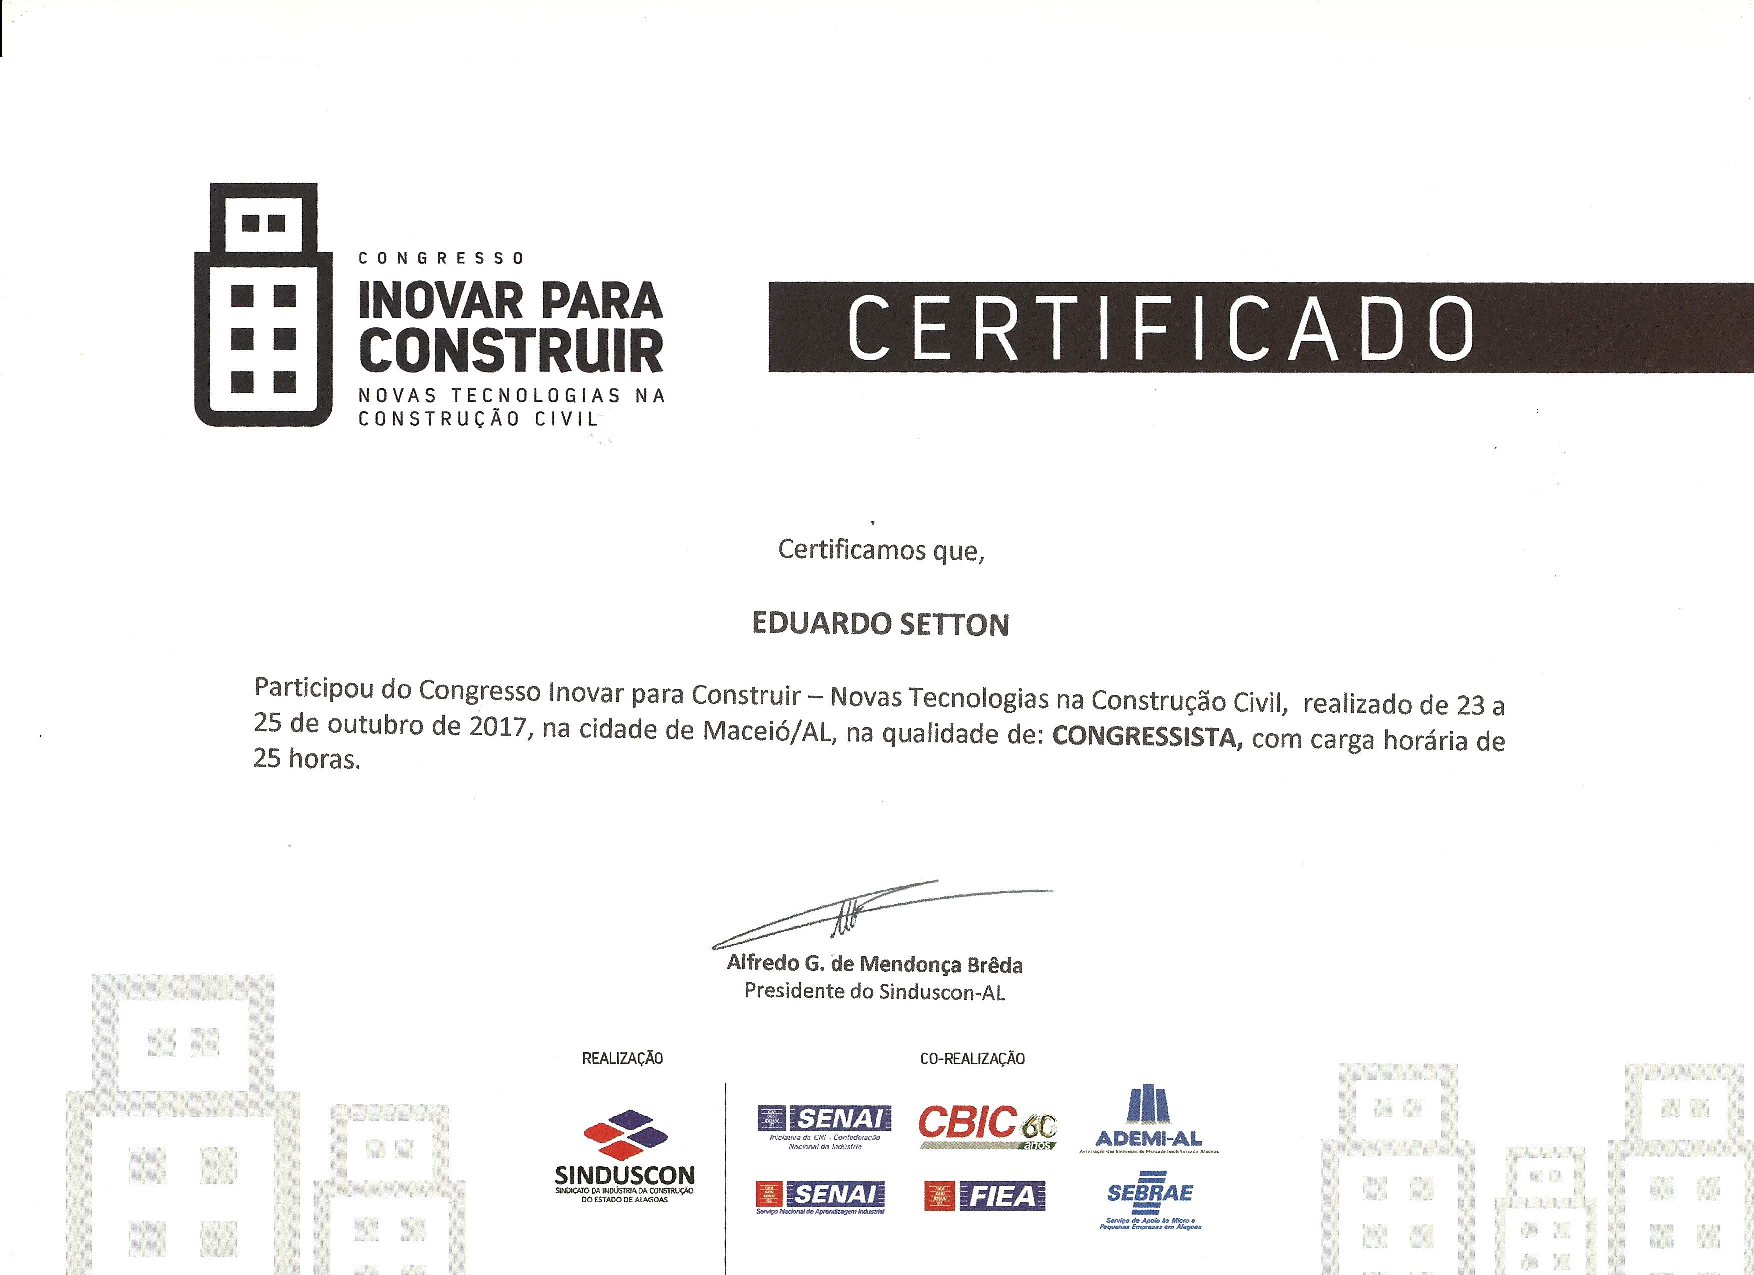
\includepdf[pages=-, scale=1, pagecommand=\thispagestyle{empty}]{\detokenize{GRUPO 2/Sub-Grupo 25/2017-inovarpconstruir}}

\subsection{Participação em eventos científicos, profissionais ou artísticos sem apresentação  de trabalho em evento nacional ou regional em apresentação de trabalho}
\label{app:2017-partpdpetro}
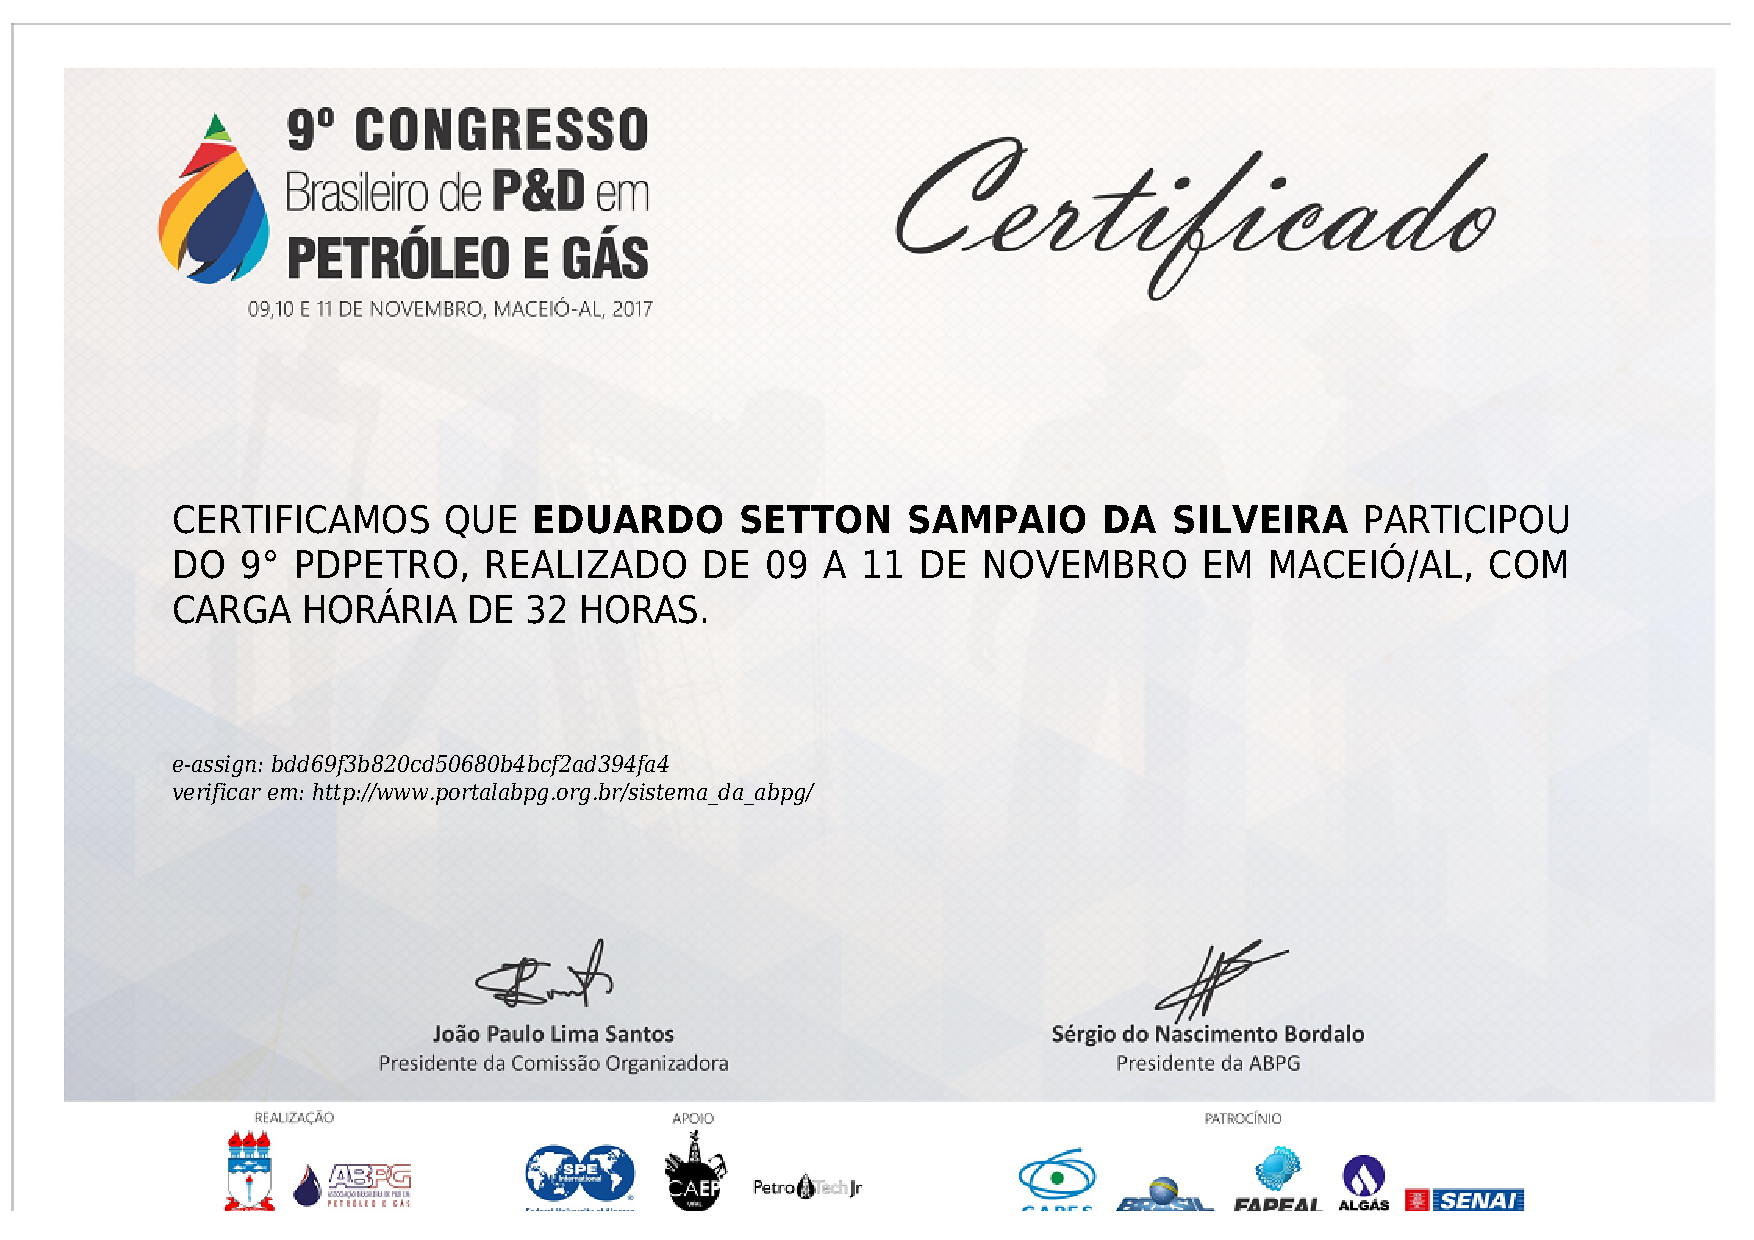
\includepdf[pages=-, scale=1, pagecommand=\thispagestyle{empty}]{\detokenize{GRUPO 2/Sub-Grupo 25/2017-partpdpetro}}

\subsection{Participação em eventos científicos, profissionais ou artísticos sem apresentação  de trabalho em evento nacional ou regional em apresentação de trabalho}
\label{app:2017-partwtdoflng}
\includepdf[pages=-, scale=1, pagecommand=\thispagestyle{empty}]{\detokenize{GRUPO 2/Sub-Grupo 25/2017-partwtdoflng}}

\subsection{Conferencista/palestrante em evento internacional}
\label{app:2016-tedx}
\includepdf[pages=-, scale=1, pagecommand=\thispagestyle{empty}]{\detokenize{GRUPO 2/Sub-Grupo 25/2016-tedx}}

\subsection{Conferencista/palestrante em evento internacional}
\label{app:2017-appwtdoflng}
\includepdf[pages=-, scale=1, pagecommand=\thispagestyle{empty}]{\detokenize{GRUPO 2/Sub-Grupo 25/2017-appwtdoflng}}

\subsection{Conferencista/palestrante em evento local}
\label{app:2016-unit}
\includepdf[pages=-, scale=1, pagecommand=\thispagestyle{empty}]{\detokenize{GRUPO 2/Sub-Grupo 25/2016-unit}}

\subsection{Conferencista/palestrante em evento local}
\label{app:2015-feac}
\includepdf[pages=-, scale=1, pagecommand=\thispagestyle{empty}]{\detokenize{GRUPO 2/Sub-Grupo 25/2015-feac}}

\subsection{Conferencista/palestrante em evento local}
\label{app:2016-brzconf1}
\includepdf[pages=-, scale=1, pagecommand=\thispagestyle{empty}]{\detokenize{GRUPO 2/Sub-Grupo 25/2016-brzconf1}}

\subsection{Conferencista/palestrante em evento local}
\label{app:2016-brzconf2}
\includepdf[pages=-, scale=1, pagecommand=\thispagestyle{empty}]{\detokenize{GRUPO 2/Sub-Grupo 25/2016-brzconf2}}

\subsection{Conferencista/palestrante em evento local}
\label{app:2016-creaal}
\includepdf[pages=-, scale=1, pagecommand=\thispagestyle{empty}]{\detokenize{GRUPO 2/Sub-Grupo 25/2016-creaal}}

\subsection{Conferencista/palestrante em evento local}
\label{app:2016-fgvsempp}
\includepdf[pages=-, scale=1, pagecommand=\thispagestyle{empty}]{\detokenize{GRUPO 2/Sub-Grupo 25/2016-fgvsempp}}

\subsection{Conferencista/palestrante em evento local}
\label{app:2016-simengpetro}
\includepdf[pages=-, scale=1, pagecommand=\thispagestyle{empty}]{\detokenize{GRUPO 2/Sub-Grupo 25/2016-simengpetro}}

\subsection{Conferencista/palestrante em evento local}
\label{app:2016-cesmac}
\includepdf[pages=-, scale=1, pagecommand=\thispagestyle{empty}]{\detokenize{GRUPO 2/Sub-Grupo 25/2016-cesmac}}

\subsection{Conferencista/palestrante em evento local}
\label{app:2016-aracomp}
\includepdf[pages=-, scale=1, pagecommand=\thispagestyle{empty}]{\detokenize{GRUPO 2/Sub-Grupo 25/2016-aracomp}}

\subsection{Conferencista/palestrante em evento local}
\label{app:2016-ceacrea}
\includepdf[pages=-, scale=1, pagecommand=\thispagestyle{empty}]{\detokenize{GRUPO 2/Sub-Grupo 25/2016-ceacrea}}

\subsection{Conferencista/palestrante em evento local}
\label{app:2016-renorbio}
\includepdf[pages=-, scale=1, pagecommand=\thispagestyle{empty}]{\detokenize{GRUPO 2/Sub-Grupo 25/2016-renorbio}}

\subsection{Conferencista/palestrante em evento local}
\label{app:2017-papotecal}
\includepdf[pages=-, scale=1, pagecommand=\thispagestyle{empty}]{\detokenize{GRUPO 2/Sub-Grupo 25/2017-papotecal}}

\subsection{Conferencista/palestrante em evento local}
\label{app:2017-cicloeng}
\includepdf[pages=-, scale=1, pagecommand=\thispagestyle{empty}]{\detokenize{GRUPO 2/Sub-Grupo 25/2017-cicloeng}}

\subsection{Conferencista/palestrante em evento local}
\label{app:2016-seconomia}
\includepdf[pages=-, scale=1, pagecommand=\thispagestyle{empty}]{\detokenize{GRUPO 2/Sub-Grupo 25/2016-seconomia}}

\subsection{Conferencista/palestrante em evento local}
\label{app:2017-unit2}
\includepdf[pages=-, scale=1, pagecommand=\thispagestyle{empty}]{\detokenize{GRUPO 2/Sub-Grupo 25/2017-unit2}}

\subsection{Conferencista/palestrante em evento local}
\label{app:2017-inform}
\includepdf[pages=-, scale=1, pagecommand=\thispagestyle{empty}]{\detokenize{GRUPO 2/Sub-Grupo 25/2017-inform}}

\subsection{Conferencista/palestrante em evento local}
\label{app:2017-sebrae}
\includepdf[pages=-, scale=1, pagecommand=\thispagestyle{empty}]{\detokenize{GRUPO 2/Sub-Grupo 25/2017-sebrae}}

\subsection{Conferencista/palestrante em evento local}
\label{app:2017-semengit}
\includepdf[pages=-, scale=1, pagecommand=\thispagestyle{empty}]{\detokenize{GRUPO 2/Sub-Grupo 25/2017-semengit}}


\subsection{Conferencista/palestrante em evento local}
\label{app:2017-cenafro}
\includepdf[pages=-, scale=1, pagecommand=\thispagestyle{empty}]{\detokenize{GRUPO 2/Sub-Grupo 25/2017-cenafro}}

\subsection{Conferencista/palestrante em evento local}
\label{app:2017-sedecmcz}
\includepdf[pages=-, scale=1, pagecommand=\thispagestyle{empty}]{\detokenize{GRUPO 2/Sub-Grupo 25/2017-sedecmcz}}


\subsection{Conferencista/palestrante em evento local}
\label{app:2017-spemovie}
\includepdf[pages=-, scale=1, pagecommand=\thispagestyle{empty}]{\detokenize{GRUPO 2/Sub-Grupo 25/2017-spemovie}}


\subsection{Debatedor/Mediador em evento nacional ou regional}
\label{app:2016-abas1}
\includepdf[pages=-, scale=1, pagecommand=\thispagestyle{empty}]{\detokenize{GRUPO 2/Sub-Grupo 25/2016-abas1}}

\subsection{Debatedor/Mediador em evento nacional ou regional}
\label{app:2016-abas2}
\includepdf[pages=-, scale=1, pagecommand=\thispagestyle{empty}]{\detokenize{GRUPO 2/Sub-Grupo 25/2016-abas2}}

\subsection{Debatedor/Mediador em evento nacional ou regional}
\label{app:2017-inovarpconstruir1}
\includepdf[pages=-, scale=1, pagecommand=\thispagestyle{empty}]{\detokenize{GRUPO 2/Sub-Grupo 25/2017-inovarpconstruir1}}

\subsection{Debatedor/Mediador em evento nacional ou regional}
\label{app:2017-mesapdpetro}
\includepdf[pages=-, scale=1, pagecommand=\thispagestyle{empty}]{\detokenize{GRUPO 2/Sub-Grupo 25/2017-mesapdpetro}}

\subsection{Debatedor/Mediador em evento local}
\label{app:2016-fundepes}
\includepdf[pages=-, scale=1, pagecommand=\thispagestyle{empty}]{\detokenize{GRUPO 2/Sub-Grupo 25/2016-fundepes}}


\subsection{Conferencista/palestrante em evento local}
\label{app:2017-aiprofnit}
\includepdf[pages=-, scale=1, pagecommand=\thispagestyle{empty}]{\detokenize{GRUPO 2/Sub-Grupo 25/2017-aiprofnit}}

\subsection{Conferencista/palestrante em evento local}
\label{app:2017-lccvnt}
\includepdf[pages=-, scale=1, pagecommand=\thispagestyle{empty}]{\detokenize{GRUPO 2/Sub-Grupo 25/2017-lccvnt}}

\subsection{Debatedor/Mediador em evento local}
\label{app:2017-aiprofnit}
\includepdf[pages=-, scale=1, pagecommand=\thispagestyle{empty}]{\detokenize{GRUPO 2/Sub-Grupo 25/2017-aiprofnit}}

\subsection{Debatedor/Mediador em evento local}
\label{app:2017-spemovie}
\includepdf[pages=-, scale=1, pagecommand=\thispagestyle{empty}]{\detokenize{GRUPO 2/Sub-Grupo 25/2017-spemovie}}


\subsection{Participação em programa/projeto de pesquisa ou desenvolvimento tecnológico, em execução, apoiado por agência de fomento ou financiado por outros}
\label{project:2017-prhanp}
\includepdf[pages=-, scale=1, pagecommand=\thispagestyle{empty}]{\detokenize{GRUPO 3/Sub-Grupo 31/2017-prhanp}}


\subsection{Criação de obras, confecção ou desenvolvimento de produtos/técnicas e de material didático}
\vspace{0.3cm}

\subsection{Desenvolvimento de software, plataforma digital ou programa computacional relacionados com a atividade acadêmica exercida pelo Docente (exceto patente)}
\label{plataforma:2017-blogeduardosetton}
\vspace{0.3cm}
\includepdf[pages=-, scale=1, pagecommand=\thispagestyle{empty}]{\detokenize{GRUPO 3/Sub-Grupo 31/2017-blogeduardosetton}}

\subsection{Desenvolvimento de material didático instrucional, exceto notas de aula}
\label{plataforma:2017-blogcursos}
\vspace{0.3cm}
\includepdf[pages=-, scale=1, pagecommand=\thispagestyle{empty}]{\detokenize{GRUPO 3/Sub-Grupo 31/2017-blogcursos}}


\subsection{Participação artística ou técnica em programa de rádio/televisão relacionado com a atividade acadêmica exercida pelo Docente}
\label{midia:2016-agendaa}
\vspace{0.3cm}
\includepdf[pages=-, scale=1, pagecommand=\thispagestyle{empty}]{\detokenize{GRUPO 2/Sub-Grupo 27/2016-agendaa}}

\subsection{Participação artística ou técnica em programa de rádio/televisão relacionado com a atividade acadêmica exercida pelo Docente}
\label{midia:2016-bomdia24jan16}
\vspace{0.3cm}
\includepdf[pages=-, scale=1, pagecommand=\thispagestyle{empty}]{\detokenize{GRUPO 2/Sub-Grupo 27/2016-bomdia24jan16}}

\subsection{Participação artística ou técnica em programa de rádio/televisão relacionado com a atividade acadêmica exercida pelo Docente}
\label{midia:2017-bomdia}
\vspace{0.3cm}
\includepdf[pages=-, scale=1, pagecommand=\thispagestyle{empty}]{\detokenize{GRUPO 2/Sub-Grupo 27/2017-bomdia}}

\subsection{Participação artística ou técnica em programa de rádio/televisão relacionado com a atividade acadêmica exercida pelo Docente}
\label{midia:2017-bloggeraldocamera1}
\vspace{0.3cm}
\includepdf[pages=-, scale=1, pagecommand=\thispagestyle{empty}]{\detokenize{GRUPO 2/Sub-Grupo 27/2017-bloggeraldocamera1}}
\includepdf[pages=-, scale=1, pagecommand=\thispagestyle{empty}]{\detokenize{GRUPO 2/Sub-Grupo 27/2017-bloggeraldocamera2}}

\subsection{Participação artística ou técnica em programa de rádio/televisão relacionado com a atividade acadêmica exercida pelo Docente}
\label{midia:2017-bomdia06dez17}
\vspace{0.3cm}
\includepdf[pages=-, scale=1, pagecommand=\thispagestyle{empty}]{\detokenize{GRUPO 2/Sub-Grupo 27/2017-bomdia06dez17}}

\subsection{Participação artística ou técnica em programa de rádio/televisão relacionado com a atividade acadêmica exercida pelo Docente}
\label{midia:2017-tedxufal}
\vspace{0.3cm}
\includepdf[pages=-, scale=1, pagecommand=\thispagestyle{empty}]{\detokenize{GRUPO 2/Sub-Grupo 27/2017-tedxufal}}

\subsection{Participação artística ou técnica em programa de rádio/televisão relacionado com a atividade acadêmica exercida pelo Docente}
\label{midia:2017-tnh130mai17}
\vspace{0.3cm}
\includepdf[pages=-, scale=1, pagecommand=\thispagestyle{empty}]{\detokenize{GRUPO 2/Sub-Grupo 27/2017-tnh130mai17}}

\subsection{Participação artística ou técnica em programa de rádio/televisão relacionado com a atividade acadêmica exercida pelo Docente}
\label{midia:2017-ministeriodopovo}
\vspace{0.3cm}
\includepdf[pages=-, scale=1, pagecommand=\thispagestyle{empty}]{\detokenize{GRUPO 2/Sub-Grupo 27/2017-ministeriodopovo}}

\subsection{Participação artística ou técnica em programa de rádio/televisão relacionado com a atividade acadêmica exercida pelo Docente}
\label{midia:2017-tnh1pausa28ago17}
\vspace{0.3cm}
\includepdf[pages=-, scale=1, pagecommand=\thispagestyle{empty}]{\detokenize{GRUPO 2/Sub-Grupo 27/2017-tnh1pausa28ago17}}

\subsection{Prestação de serviços e assistência técnica}
\label{ptec:2017-r1dynasim}
\vspace{0.3cm}
\includepdf[pages=-, scale=1, pagecommand=\thispagestyle{empty}]{\detokenize{GRUPO 2/Sub-Grupo 28/2017-r1dynasim}}

\subsection{Prestação de serviços e assistência técnica}
\label{ptec:2017-r2dynasim}
\vspace{0.3cm}
\includepdf[pages=-, scale=1, pagecommand=\thispagestyle{empty}]{\detokenize{GRUPO 2/Sub-Grupo 28/2017-r2dynasim}}

\subsection{Outras Atividades Correlatas}
\label{outras:2016-agendaa}
\vspace{0.3cm}
\includepdf[pages=-, scale=1, pagecommand=\thispagestyle{empty}]{\detokenize{GRUPO 2/Sub-Grupo 29/2016-agendaa}}

\subsection{Outras Atividades Correlatas}
\label{outras:2017-tedxufal}
\vspace{0.3cm}
\includepdf[pages=-, scale=1, pagecommand=\thispagestyle{empty}]{\detokenize{GRUPO 2/Sub-Grupo 29/2017-tedxufal}}

\subsection{Outras Atividades Correlatas}
\label{outras:2016-fiea}
\vspace{0.3cm}
\includepdf[pages=-, scale=1, pagecommand=\thispagestyle{empty}]{\detokenize{GRUPO 2/Sub-Grupo 29/2016-fiea}}

\subsection{Outras Atividades Correlatas}
\label{outras:2016-orgsnct}
\vspace{0.3cm}
\includepdf[pages=-, scale=1, pagecommand=\thispagestyle{empty}]{\detokenize{GRUPO 2/Sub-Grupo 29/2016-orgsnct}}

\subsection{Outras Atividades Correlatas}
\label{outras:2016-doccesmac}
\vspace{0.3cm}
\includepdf[pages=-, scale=1, pagecommand=\thispagestyle{empty}]{\detokenize{GRUPO 2/Sub-Grupo 29/2017-doccesmac}}

\subsection{Outras Atividades Correlatas}
\label{outras:2017-sefaz}
\vspace{0.3cm}
\includepdf[pages=-, scale=1, pagecommand=\thispagestyle{empty}]{\detokenize{GRUPO 2/Sub-Grupo 29/2017-sefaz}}

\subsection{Programas/projetos de pesquisa}
\vspace{0.3cm}

\subsection{Coordenação de Programa/Projeto de pesquisa ou desenvolvimento tecnológico, em execução, apoiado por agência de fomento ou financiado por outros}
\label{coordproject:2017-fundepes}
\vspace{0.3cm}
\includepdf[pages=-, scale=1, pagecommand=\thispagestyle{empty}]{\detokenize{GRUPO 3/Sub-Grupo 31/2017-fundepes}}


\subsection{Participação em programa/projeto de pesquisa ou desenvolvimento tecnológico, em execução, apoiado por agência de fomento ou financiado por outros}
\label{partproject:2017-fundepes}
\vspace{0.3cm}
\includepdf[pages=-, scale=1, pagecommand=\thispagestyle{empty}]{\detokenize{GRUPO 3/Sub-Grupo 31/2017-fundepes}}

\subsection{Coordenação de Programa/Projeto de pesquisa ou desenvolvimento tecnológico, em execução, apoiado por agência de fomento ou financiado por outros}
\label{project:2017-ecoefici}
\vspace{0.3cm}
\includepdf[pages=-, scale=1, pagecommand=\thispagestyle{empty}]{\detokenize{GRUPO 3/Sub-Grupo 31/2017-ecoefici}}

\subsection{Coordenação de programa/projeto de pesquisa ou desenvolvimento tecnológico, devidamente aprovado na Unidade Acadêmica/Campus e registrado na PROPEP}
\label{part:2017-projpesquisa}
\vspace{0.3cm}
\includepdf[pages=-, scale=1, pagecommand=\thispagestyle{empty}]{\detokenize{GRUPO 3/Sub-Grupo 31/2017-pibit}}



%%%%%%%%%%%%%%%%%%%%%%%%%%%%%%%%%%%%%%%%%%%%%%%%%%%%%%%%%%%%%%%%%%%%%%%%%%%%%%%
% \newpage
% \subsection{Portaria de Progressão}
% \label{app:2014-portaria-progressao}
% \includepdf[pages=-, scale=1,pagecommand=\thispagestyle{empty}]{\detokenize{GRUPO 1/20141205_Portaria-de-Progressao-Funcional_5929-2014.pdf}}

\end{document}

%%% EOF
